\documentclass[11pt]{report}

\usepackage[T1]{fontenc}
% Nicer default font (+ math font) than Computer Modern for most use cases
\usepackage{mathpazo}

% Basic figure setup, for now with no caption control since it's done
% automatically by Pandoc (which extracts ![](path) syntax from Markdown).
\usepackage{graphicx}
% We will generate all images so they have a width \maxwidth. This means
% that they will get their normal width if they fit onto the page, but
% are scaled down if they would overflow the margins.
\makeatletter
\def\maxwidth{\ifdim\Gin@nat@width>\linewidth\linewidth
\else\Gin@nat@width\fi}
\makeatother
\let\Oldincludegraphics\includegraphics

\usepackage{color}

\usepackage{xcolor} % Allow colors to be defined
\usepackage{enumerate} % Needed for markdown enumerations to work
\usepackage{amsmath} % Equations
\usepackage{amssymb} % Equations
\usepackage{textcomp} % defines textquotesingle
% Hack from http://tex.stackexchange.com/a/47451/13684:
\AtBeginDocument{%
    \def\PYZsq{\textquotesingle}% Upright quotes in Pygmentized code
}
\usepackage{upquote} % Upright quotes for verbatim code
\usepackage[mathletters]{ucs} % Extended unicode (utf-8) support
\usepackage[utf8x]{inputenc} % Allow utf-8 characters in the tex document
\usepackage{fancyvrb} % verbatim replacement that allows latex

% The hyperref package gives us a pdf with properly built
% internal navigation ('pdf bookmarks' for the table of contents,
% internal cross-reference links, web links for URLs, etc.)
\usepackage{hyperref}

\usepackage{fleqn}
\usepackage{placeins}
\usepackage{epsfig}
\usepackage{a4wide}
\usepackage{wasysym}
\usepackage{stmaryrd}
\usepackage{alltt}
\usepackage{theorem}
\usepackage{minted}
\usepackage{makeidx}

\usepackage{hyperref}
\usepackage[all]{hypcap}
\hypersetup{
  colorlinks = true, 
  linkcolor  = blue,
  citecolor  = red,
  filecolor  = Gold,
  urlcolor   = [rgb]{0.5, 0.0, 0.5},
  pdfborder  = {0 0 0} 
}

\usepackage{fancyhdr}
\usepackage{lastpage} 

% Colors for the hyperref package
\definecolor{urlcolor}{rgb}{0.5,0,0.5}
\definecolor{linkcolor}{rgb}{0.0,0.0,1.0}
\definecolor{citecolor}{rgb}{.12,.54,.11}
\definecolor{ttcolor}{rgb}{0.4,0.1,0.0}

\definecolor{darkgreen}{rgb}{0.0, 0.0, 0.8}
\definecolor{puregreen}{rgb}{0.0, 1.0, 0.0}
\definecolor{darkred}{rgb}{0.6, 0.0, 0.0}

\newcommand{\tsq}[1]{\textquotesingle#1\textquotesingle} 
\newcommand{\blue}[1]{{\color{blue}#1}}
\newcommand{\green}[1]{{\color{darkgreen}#1}}
\newcommand{\puregreen}[1]{\colorbox{brown}{\color{puregreen}#1}}
\newcommand{\red}[1]{{\color{darkred}#1}}
\newcommand{\mytt}[1]{{\color{ttcolor}\texttt{#1}}}
\pagestyle{fancy}

\fancyfoot[C]{--- \thepage/\pageref{LastPage}\ ---}

\fancypagestyle{plain}{%
\fancyhf{}
\fancyfoot[C]{--- \thepage/\pageref{LastPage}\ ---}
\renewcommand{\headrulewidth}{0pt}
}

\fancyheadoffset{0.1cm}
\renewcommand{\chaptermark}[1]{\markboth{\chaptername \ \thechapter.\ #1}{}}
\renewcommand{\sectionmark}[1]{\markright{\thesection. \ #1}{}}
\fancyhead[R]{\leftmark}
\fancyhead[L]{\rightmark}

\definecolor{amethyst}{rgb}{1.0, 0.7, 0.4}
\definecolor{orange}{rgb}{1, 0.9, 0.0}
\definecolor{sepia}{rgb}{1.0,1.0,0.9}

\setlength{\mathindent}{1.3cm}
\setlength{\textwidth}{17cm}
\addtolength{\oddsidemargin}{-1cm}
\addtolength{\evensidemargin}{-1cm}
\addtolength{\topmargin}{-1cm}


\setlength{\mathindent}{1.3cm}
\setlength{\topsep}{0.1cm plus0.1cm minus 0.0cm}
\setlength{\partopsep}{0.0cm plus0.1cm minus 0.0cm}
\setlength{\parsep}{0.1cm plus0.1cm minus 0.0cm}
\setlength{\parskip}{0.1cm plus0.1cm minus 0.0cm}
\newfont{\chess}{chess20}
\newfont{\bigchess}{chess30}
\newcommand{\chf}{\baselineskip20pt\lineskip0pt\chess}
\newcommand{\ds}{\displaystyle}
\newcommand{\diff}{\frac{\textrm{d}\;\;}{\textrm{d}\mbox{$x$}}}

{\theorembodyfont{\slshape}
\newtheorem{Definition}{Definition}
\newtheorem{Notation}[Definition]{Notation}
\newtheorem{Korollar}[Definition]{Korollar}
\newtheorem{Corollary}[Definition]{Corollary}
\newtheorem{Lemma}[Definition]{Lemma}
\newtheorem{Proposition}[Definition]{Proposition}
\newtheorem{Satz}[Definition]{Satz}
\newtheorem{Theorem}[Definition]{Theorem}
}

\hyphenation{com-pre-hen-sion}
% set the monospace-font to Inconsalata-g
% font-source: http://leonardo-m.livejournal.com/77079.html

\title{\epsfig{file=dhbw-logo.eps, scale=1.2}  \\[0.2cm]
       Theoretical Computer Science: \\
       An Introduction to Logic via \textsl{Python} \\[0.3cm]
      --- Spring 2025 ---     \\[0.3cm]
      Baden-Wuerttemberg Cooperative State University (DHBW)}
\author{Prof.~Dr.~Karl Stroetmann}


\date{\today \\[0.5cm]
\begin{minipage}[t]{1.0\linewidth}
\noindent
These lecture notes, the corresponding \LaTeX\ sources and the programs discussed in these lecture notes are available at
\\[0.2cm]
\hspace*{\fill}
\href{https://github.com/karlstroetmann/Logic}{\texttt{https://github.com/karlstroetmann/Logic}}.
\hspace*{\fill} 
\\[0.2cm]
The \href{https://github.com/karlstroetmann/Logic/blob/master/Lecture-Notes/logic.pdf}{lecture notes}
can be found in the directory
\href{https://github.com/karlstroetmann/Logic/blob/master/Lecture-Notes}{\texttt{Lecture-Notes}}
in the file
\href{https://github.com/karlstroetmann/Logic/blob/master/Lecture-Notes/logic.pdf}{\texttt{logic.pdf}}.
The \href{https://jupyter-notebook.readthedocs.io/en/stable/}{Jupyter Notebooks} discussed in this lecture 
are found in the directory \href{https://github.com/karlstroetmann/Logic/blob/master/Python}{\texttt{Python}}.
These lecture notes are revised occasionally.   To automatically update the lecture notes,  you can install
the program \href{http://git-scm.com/download}{\texttt{git}}.  Then, using the command line of your favourite
operating system, you can \blue{clone} my repository using the command  
\\[0.2cm]
\hspace*{1.3cm}
\texttt{git clone https://github.com/karlstroetmann/Logic.git}.
\\[0.2cm]
Once the repository has been cloned, it can be \blue{updated} using the command
\\[0.2cm]
\hspace*{1.3cm}
\texttt{git pull}.
\\[0.2cm]
As the lecture notes are constantly changing, you should do so regularly.
\end{minipage}
}

\newcommand{\quoted}[1]{\texttt{\symbol{34}\texttt{#1}\symbol{34}}}
\newcommand{\schluss}[2]{\frac{\displaystyle\quad \rule[-6pt]{0pt}{12pt}#1 \quad}{\displaystyle\quad \rule{0pt}{10pt}#2 \quad}}
\newcommand{\bruch}[2]{\frac{\displaystyle#1}{\displaystyle #2}}
\newcommand{\vschlus}[1]{{\displaystyle\rule[-6pt]{0pt}{12pt} \atop \rule{0pt}{10pt}#1}}

\newcommand{\example}{\vspace*{0.2cm}

\noindent
\textbf{Beispiel}: \ }

\newcommand{\exampleEng}{\vspace*{0.2cm}

\noindent
\textbf{Example}: \ }

\newcommand{\examples}{\vspace*{0.2cm}

\noindent
\textbf{Beispiele}: \ }

\newcommand{\examplesEng}{\vspace*{0.2cm}

\noindent
\textbf{Examples}: \ }

\newcommand{\next}{\vspace*{0.2cm}

\noindent}

\newcommand{\remark}{\vspace*{0.2cm}

\noindent
\textbf{Bemerkung}: }

\newcommand{\remarks}{

\noindent
\textbf{Bemerkung}: }

\newcommand{\remarkEng}{\vspace*{0.2cm}

\noindent
\textbf{Remark}: }


\newcounter{aufgabe}
\newcommand{\exercise}{\vspace*{0.1cm}
\stepcounter{aufgabe}

\noindent
\textbf{Aufgabe \arabic{aufgabe}}: }

\newcommand{\exerciseEng}{\vspace*{0.1cm}
\stepcounter{aufgabe}

\noindent
\textbf{Exercise \arabic{aufgabe}}: }

\newcommand{\solution}{\vspace*{0.2cm}

\noindent
\textbf{L\"{o}sung}: \ }

\newcommand{\solutionEng}{\vspace*{0.2cm}

\noindent
\textbf{Solution}: \ }

\newcommand{\proof}{\vspace*{0.2cm}

\noindent
\textbf{Proof}: }

\newcommand{\mycheck}{\green{$\surd$}}
\newcommand{\dv}{\mbox{\,\mytt{/}$\!$\mytt{/}\,}}
\newcommand{\dvv}{\mbox{\scriptsize\,\mytt{/}$\!$\mytt{/}\,}}
\newcommand{\mmod}{\,\texttt{\%}\,}
\newcommand{\mdiv}{\,\texttt{//}\,}
\newcommand{\lb}{\hspace*{\fill} \linebreak}
\newcommand{\modulo}{\;\texttt{\%}\;}
\newcommand{\qed}{\hspace*{\fill} $\Box$}
\newcommand{\eox}{\hspace*{\fill} $\diamond$}
\newcommand{\exend}{\hspace*{\fill} $\diamond$}
\newcommand{\setl}{\textsc{SetlX}}
\newcommand{\setlx}{\textsc{SetlX}}
\newcommand{\struct}{\mathcal{S}}
\newcommand{\FV}{\textsl{FV}}
\newcommand{\id}{\textrm{id}}
\newcommand{\dom}{\textrm{dom}}
\newcommand{\rng}{\textrm{rng}}
\newcommand{\BV}{\textsl{BV}}
\newcommand{\var}{\textsl{Var}}
\newcommand{\el}{\!\in\!}
\newcommand{\at}{\texttt{\symbol{64}}}
\newcommand{\notel}{\!\not\in\!}
\newcommand{\I}{\mathcal{I}}
\newcommand{\verum}{\top}
\newcommand{\falsum}{\bot}
\newcommand{\gentzen}{\vdash}
\newcommand{\komplement}[1]{\overline{\,#1\,}}
\newcommand{\mathquote}[1]{\mbox{``}\mathtt{#1}\mbox{''}}
\newcommand{\squote}[1]{\symbol{34}\texttt{#1}\symbol{34}}

\newcommand{\circneg}{\mbox{$\bigcirc\hspace*{-0.36cm}\neg$}}
\newcommand{\circwedge}{\mbox{$\bigcirc\hspace*{-0.34cm}\wedge$}}
\newcommand{\circvee}{\mbox{$\bigcirc\hspace*{-0.34cm}\vee$}}
\newcommand{\circright}{\mbox{$\bigcirc\hspace*{-0.52cm}\rightarrow$}}
\newcommand{\circleftright}{\mbox{$\bigcirc\hspace*{-0.52cm}\leftrightarrow$}}
\newcommand{\club }{\ensuremath{\clubsuit   }}
\newcommand{\spade}{\ensuremath{\spadesuit  }}
\newcommand{\heart}{\ensuremath{\heartsuit  }}
\newcommand{\diamo}{\ensuremath{\diamondsuit}}

\newcommand{\hoare}[3]{\bigl\{#1\bigr\}\quad\texttt{#2}\quad\bigl\{#3\bigr\}}
\newcommand{\Oh}{\mathcal{O}}

\newcommand{\myfig}[1]{Abbildung \ref{fig:#1} auf Seite \pageref{fig:#1}}
\newcommand{\myFig}[1]{Figure \ref{fig:#1} on page \pageref{fig:#1}}

\def\pair(#1,#2){\langle #1, #2 \rangle}

\makeindex

\begin{document}
\maketitle
\tableofcontents
\chapter{Introduction}
For the uninitiated, \href{https://en.wikipedia.org/wiki/Mathematical_logic}{mathematical logic} 
is both quite abstract and pretty arcane.  
In this short chapter, I would like to motivate why you have to learn
logic in order to become a computer scientist.  After that, I will give a short overview of the topics covered
in this lecture.

\section{Motivation}
In the lecture on \href{https://github.com/karlstroetmann/Algorithms/blob/master/Lecture-Notes/algorithms.pdf}{algorithms},
we have discussed three important properties that an algorithms should have:
An algorithm should be
\begin{itemize}
\item correct,
\item efficient, and
\item simple.  
\end{itemize}
The efficiency of algorithms has been discussed in the lecture on algorithms.  This lecture will
therefore focus on the correctness of algorithms.  The rest of this section will further motivate the
importance of the correctness of algorithms. 

Modern software systems are among the most complex systems developed by mankind.  You can get a
sense of the complexity of these systems if you look at the amount of work that is necessary to
build and maintain complex software systems.  Today it is quite common that complex software projects require
more than a thousand developers.  Of course, the failure of a project of this size is very costly and can have
catastrophic consequences.  Nevertheless, history shows that these failures happen.
Here is a list of software problems that have made it to the headlines in recent years.
\begin{enumerate}
\item A stark example of IT failure consequences is the
      \href{https://www.npr.org/2023/01/26/1151667801/southwest-airlines-investigation-losses-holiday-travel-cancellations}{December 2022 Southwest Airlines meltdown}.
      A number of delayed flights due to a severe winter storm triggered the collapse of the Southwest Airlines
      crew scheduling system \blue{SkySolver}, leading to over 16,700 
      canceled flights and stranding hundreds of thousands of passengers during peak holiday travel. Southwest
      estimated the financial impact at over \$1 billion. 
\item In 2018 and 2019 two Boeing 737 MAX planes crashed because of a software problem in the
      \href{https://en.wikipedia.org/wiki/Maneuvering_Characteristics_Augmentation_System}{Maneuvering
        Characteristics Augmentation System}.
      
      This error lead to the death of 346 passengers and crew.
\item Between 1999 and 2015 the British Post Office used a faulty accounting software provided by Fujitsu.
      As a result of the buggy accounting, over 900 employees of the British Post Office were falsely
      convicted of embezzlement.  As a consequences, some of these employees were imprisoned.  Four of those
      that were falsely convicted committed suicide.  These tragic incidents are know as the
      \href{https://en.wikipedia.org/wiki/British_Post_Office_scandal}{Horizon IT scandal}.     
\item In 1996, the very first Ariane 5 rocket self-destructed as a result of a
      \href{https://www.bugsnag.com/blog/bug-day-ariane-5-disaster/}{software error}. 
\end{enumerate}
These and numerous other examples show that the development of complex software systems requires a high level
of precision and diligence.  Hence, the development of software needs a solid scientific
foundation.  \href{https://en.wikipedia.org/wiki/Mathematical_logic}{Mathematical logic} 
is an important part of this foundation that has immediate applications in computer science. 
\begin{enumerate}[(a)]
\item Logic can be used to specify the \blue{interfaces} of complex systems.  
\item Logic is used to build interactive theorem provers that are able to establish the correctness of
      software.  For example, \textsl{MicroSoft}\textsuperscript{TM} has build the
      \href{https://leanprover.github.io}{Lean Prover} and the
      \href{https://www.microsoft.com/en-us/research/project/z3-3/}{Z3}, which is a logic constraint solver, as
      part of their 
      \href{https://www.microsoft.com/en-us/research/group/research-software-engineering-rise/}{research in
        software engineering}. 
\item The correctness of digital circuits can be verified using \blue{automatic theorem provers} that are based on
      propositional logic.  For example, \textsl{Cadence}\textsuperscript{TM} has built the
      \href{https://www.cadence.com/en_US/home/tools/system-design-and-verification/formal-and-static-verification.html}{Jasper
        Formal Verification Platform}.
\end{enumerate}
It is easy to extend this enumeration.  However, besides their immediate applications, 
there is another reason you have to study both logic and set theory: Without the proper use of
{\color{blue}abstractions}, complex software systems cannot be managed.  After all, nobody is able to keep
millions of lines of program code in her head.  The only way to construct and manage a software system of this
size is to introduce the right abstractions and to develop the system in layers.  Hence, the ability
to work with abstract concepts is one of the main virtues of a modern computer scientist.  
Exposing students to mathematics in general and logic in particular trains their abilities to grasp abstract concepts.

From my past teaching experience I know that many students think that a good programmer already is a
good computer scientist.  In reality, we have
\\[0.2cm]
\hspace*{1.3cm}
$\textrm{good programmer} \not= \textrm{good computer scientist}$.
\\[0.2cm]
This should not be too surprising.  After all, there is no reason to believe that a good bricklayer is a good
architect and neither is a good architect necessarily a good bricklayer.
In computer science, a good programmer need not be a scientist at all, while a {\color{blue}computer
  \underline{scientist}}, by its very name, is a {\color{blue}scientist}.  
There is no denying that {\color{blue}mathematics} in general and 
{\color{blue}logic} in particular is an important part of science.  Furthermore, these topics form the
foundation of computer science.  Therefore, you should master them.  In addition, this
part of your scientific education is much more permanent than the knowledge of any particular programming
language.  Nobody knows which programming language will be \emph{en vogue} in 10 years from now.  In three 
years, when you start your professional career, most of you will have to learn new
programming languages.   Then your ability to quickly grasp new concepts will be much more important than your
skills in any particular programming language. 

\section{Overview} 
This lecture deals mostly with mathematical logic and is structured as follows.
\begin{enumerate}[(a)]
\item We begin our lecture by investigating the limits of computability.

      For certain problems there is no algorithm that can solve the problem algorithmically. 
      For example, the question whether a given program will \blue{terminate} for a given input is not
      \blue{decidable}.  This is known as the \href{https://en.wikipedia.org/wiki/Halting_problem}{halting problem}.  
      We will prove the \blue{undecidability} of the halting problem in the second chapter. 
\item The third chapter discusses two different methods that can be used to prove the correctness of a program:
      \begin{itemize}
      \item \blue{Computational induction} is the method of choice for proving the correctness of recursive
            algorithms.
      \item \blue{Symbolic verification} is used to verify iterative algorithms.
      \end{itemize}
\item The fourth chapter discusses \href{https://en.wikipedia.org/wiki/Propositional_calculus}{propositional logic}.

      In logic, we distinguish between  \blue{propositional logic},
      \blue{first order logic}, and \blue{higher order logic}.  \blue{Propositional} logic is only
      concerned with the \blue{logical connectives}
      \begin{itemize}
      \item $\neg$ (not), 
      \item $\wedge$ (and),
      \item $\vee$ (or),
      \item $\rightarrow$ (if $\cdots$ then),
      \item $\leftrightarrow$ (if and only if).
      \end{itemize}
      \blue{First-order logic} also investigates the \blue{quantifiers}
      \begin{itemize}
      \item $\forall$ (for all),
      \item $\exists$ (there exists).
      \end{itemize}
      where these quantifiers range over the objects of the \blue{domain of discourse}.
      Finally, in \blue{higher order logic} these quantifiers also range over \blue{sets}, \blue{functions}, and
      \blue{predicates}. 

      As propositional logic is easier to grasp than first-order logic, we start our investigation
      of logic with propositional logic.  Furthermore, propositional logic has the advantage of
      being \blue{decidable}:  We will present an algorithm that can check whether a propositional formula
      is satisfiable.  In contrast to propositional logic, first-order logic is not decidable.

      Next, we discuss applications of propositional logic:  We will show how the \blue{8 queens problem} 
      can be reduced to the question whether a formula from propositional logic is satisfiable.  We present
      the algorithm of \blue{Davis and Putnam} that can decide the satisfiability of a propositional formula.
      and, for example, is able to solve the 8 queens problem.  
\item Finally, we discuss \href{https://en.wikipedia.org/wiki/First-order_logic}{first-order logic}.

      The most important concept of the last chapter will be the notion of a \blue{formal proof} in
      first order logic.  To this end, we introduce a \blue{formal proof system} that is
      \blue{complete} for first order logic.  \blue{Completeness} means that we will develop an
      algorithm that can \blue{prove} the correctness of every first-order formula that is
      universally valid.  This algorithm is the foundation of \blue{automated theorem proving}.

      As an application of theorem proving we discuss the systems \href{https://vprover.github.io/}{Vampire},
      \href{https://www.cs.unm.edu/~mccune/mace4/}{Prover9} and
      \href{https://www.cs.unm.edu/~mccune/mace4/}{Mace4}. \blue{Prover9} is an automated theorem prover, while
      \blue{Mace4} can be used to refute a mathematical conjecture.
\end{enumerate}

\section{Chapter Review}
\begin{itemize}
\item Provide three examples of faulty software systems that have caused great harm.
      Do not cote the examples given in this Chapter but rather search the web to find more examples.
\item Provide two examples of automatic theorem provers that are used in industry.
\item Is first order logic more expressive as propositional logic or is it the other way around?
\end{itemize}


%%% Local Variables: 
%%% mode: latex
%%% TeX-master: "logic"
%%% End: 

%\chapter{Naive Set Theory}
The concept of \href{https://en.wikipedia.org/wiki/set_theory}{set theory} has arisen towards the end of the 19th century
from an effort to put mathematics on a solid foundation.  The creation of a solid foundation was considered necessary as
the concept of \emph{infinity} increasingly worried mathematicians. 

The essential parts of set theory have been defined by \href{https://de.wikipedia.org/wiki/Georg_Cantor}{Georg
  Cantor} \index{Cantor, Georg} (1845 -- 1918). The first definition of the concept of a set was approximately as follows
\cite{cantor:1895}: 

\begin{center}
\colorbox{red}{\framebox{\colorbox{yellow}{
\begin{minipage}{0.85\linewidth}
  A ``set'' \index{set} is a \blue{well-defined} collection $M$ of certain objects $x$ of our perception or our thinking.
\end{minipage}}}}
\end{center}
\vspace*{0.2cm}

\noindent
Here, the attribute ``\blue{well-defined}'' expresses the fact that for a given quantity $M$ and an object $x$ we have
to be able to decide whether the object $x$ belongs to the set $M$.  If $x$ belongs to $M$, then $x$ is called an
\blue{element} of the set $M$ and we write this as
\\[0.2cm]
\hspace*{1.3cm}
$x \in M$ \quad (read: $x$ is an element of $M$). 
\\[0.2cm]
Slightly abbreviated we can define the notion of a set as follows: 
\\[0.2cm]
\hspace*{1.3cm}
\textsl{A set is a \blue{well-defined} collection of elements}.
\\[0.2cm]
To mathematically understand the concept of a \blue{well-defined collection of elements},
Cantor introduced the so-called \index{comprehension, axiom of unrestricted} \blue{axiom of unrestricted comprehension}.
We can formalize this axiom as follows:  If $p(x)$ is a \blue{property} that
an object $x$ can have, we can define the set $M$ of all objects that have this
property.  Therefore, the set $M$ can be defined as 
\\[0.2cm]
\hspace*{1.3cm} 
$M := \{ x \;|\; p(x) \}$ \quad (read: ``$M$ is the set of all those $x$ such that $p(x)$ holds'').
\\[0.2cm]
Here, the property $p(x)$ is just a formula in which the variable $x$ happens to appear.
We illustrate the axiom of comprehension by an example: If $\mathbb{N}$ is
the set of natural numbers, then we can define the set of all \emph{even} natural numbers
via the property \\[0.2cm]
\hspace*{1.3cm} $p(x) \;:=\; (\exists y\in \mathbb{N}: x = 2 \cdot y)$. \\[0.2cm]
Using this property, the set of even natural numbers can be defined as \\[0.2cm]
\hspace*{1.3cm} $\{ x \;|\; \exists y\in \mathbb{N}: x = 2 \cdot y \}$. 

Unfortunately, the unrestricted use of the axiom of comprehension leads to serious problems.  To give an
example, let us consider the property of a set to \underline{not} contain itself.  We define the property
$p(x)$ as
\\[0.2cm]
\hspace*{1.3cm}
 $p(x) := \neg(x \in x)$ 
\\[0.2cm]
and proceed to define the set $R$ of all sets $x$ that do not contain themselves as follows:
\\[0.2cm]
\hspace*{1.3cm} 
$R := \{ x \;|\; \neg (x \in x) \}$.  
\\[0.2cm]
Intuitively, we might expect that no set can contain itself.  However, things turn out to be more complicated.
Let us try to check whether the set $R$ contains itself.  We have
\\[0.2cm]
\hspace*{1.3cm}
$
\begin{array}{cl}
                  & R \in R \\[0.2cm] 
  \Leftrightarrow & R \in \bigl\{ x \;|\; \neg (x \in x) \bigr\} \\[0.2cm] 
  \Leftrightarrow & \neg (R \in R).
\end{array}
$
\\[0.2cm]
So we have shown that
\\[0.2cm]
\hspace*{1.3cm}
$R \in R \;\Leftrightarrow\; \neg(R \in R)$
\\[0.2cm]
holds.  In other words, the set $R$ is a member of itself if and only if $R$ is not a member of itself!
Obviously, this is a contradiction.  As a way out, we can only conclude that the expression \\[0.2cm]
\hspace*{1.3cm} $\{ x \mid \neg (x \in x) \}$ \\[0.2cm]
\blue{does not define a set}.  This shows that the axiom of comprehension is too general:  Not every expression of the form 
\\[0.2cm] 
\hspace*{1.3cm}
$M := \{ x \mid p(x) \}$ 
\\[0.2cm]
defines a set.  The expression
\\[0.2cm]
\hspace*{1.3cm}
$\bigl\{x \mid \neg(x \in x)\bigr\}$
\\[0.2cm]
has been discovered by the British logician and philosopher 
\index{Russell, Bertrand}
\href{http://de.wikipedia.org/wiki/Bertrand_Russell}{Bertrand Russell} (1872 -- 1970).  It is known as
\href{http://de.wikipedia.org/wiki/Russellsche_Antinomy}{Russell's Antinomy}. 
\index{Russell's Antinomy, $\{x \mid x \not\in x\}$}

In order to avoid \emph{paradoxes} such as Russell's antinomy, it is necessary to be more careful when sets are
constructed.  In the following, we will present methods to construct sets that are less powerful than the 
axiom of comprehension, but, nevertheless, these methods will be sufficient for our purposes.  We will continue
to use the notation underlying the comprehension axiom and write set definitions in the form
\\[0.2cm]
\hspace*{1.3cm}
$M = \{ x \mid p(x) \}$. \qquad (read: $M$ is the set of all $x$ such that $p(x)$ holds.)  
\\[0.2cm]
However, we won't be allowed to use arbitrary formulas $p(x)$ here.  Instead, the formulas we are going to use
for $p(x)$ have to satisfy some \emph{restrictions}.  These restrictions will prevent the construction of
self-contradictory sets.


\section{Defining Sets by Listing their Elements}
The simplest way to define a set is to list of all of its elements. These elements are enclosed in the
curly braces  ``\texttt{\{}'' and ``\texttt{\}}'' and are separated by commas.
For example, when we define \\[0.2cm]
\hspace*{1.3cm} $M := \{ 1, 2, 3 \}$, \\[0.2cm]
then the set $M$ contains the elements $1$, $2$ and $3$.
Using  the notation of the axiom of unrestricted comprehension we could write this set as \\[0.2cm]
\hspace*{1.3cm} 
$M = \{ x \mid x = 1 \vee x = 2 \vee x = 3 \}$.
\\[0.2cm]
Another example of a set that can be created by explicitly enumerating its elements
is the set of all lower case Latin characters.  This set is given as
define: \\[0.2cm]
\hspace*{1.3cm} 
$\{\mathtt{a}, \mathtt{b}, \mathtt{c}, \mathtt{d}, \mathtt{e},
 \mathtt{f}, \mathtt{g}, \mathtt{h}, \mathtt{i}, \mathtt{j}, \mathtt{k}, \mathtt{l},
 \mathtt{m}, \mathtt{n}, \mathtt{o}, \mathtt{p}, \mathtt{q}, \mathtt{r}, \mathtt{s},
 \mathtt{t}, \mathtt{u}, \mathtt{v}, \mathtt{w}, \mathtt{x}, \mathtt{y}, \mathtt{z}\}$.
 \\[0.2cm]
Occasionally, we will use \blue{dots notation} to define a set.  Using dots notation, the set of all lower case
elements is written as
\\[0.2cm]
\hspace*{1.3cm}
$\{ \mathtt{a}, \mathtt{b}, \mathtt{c}, \cdots, \mathtt{x}, \mathtt{y}, \mathtt{z}\} $.
\\[0.2cm]
Of course, if we use dots notation the interpretation of the dots ``$\cdots$'' must always be obvious from the
context of the definition. 

As a last example, we consider the \blue{empty set} $\emptyset$, which is defined as
\index{empty set, $\emptyset$}
\\[0.2cm]
\hspace*{1.3cm}
$\emptyset := \{\}$.
\\[0.2cm]
Therefore, the empty set does not contain any element at all.  This set plays an important role in set theory which
is similar to the role played by the number $0$ in algebra.

If a set is defined by listing all of its elements, the order in which the
elements are listed is \blue{not} important.  For example, we have
\\[0.2cm]
\hspace*{1.3cm}
$\{1,2,3\} = \{3,1,2\}$,
\\[0.2cm]
since both sets contain the same elements.   
This is summarized as the statement that 
\\[0.2cm]
\hspace*{1.3cm}
\blue{a set abstracts from the order of its elements}. 


\section{Predefined Infinite Sets of Numbers}
All sets that are defined by explicitly listing their elements can only have finitely many elements.  
In mathematics there are some sets that have an \blue{infinite} number of
elements.  One example is the 
\href{http://en.wikipedia.org/wiki/Natural_number}{set of natural numbers}, \index{set of natural numbers, $\mathbb{N}$} 
which is denoted by the symbol $\mathbb{N}$.
Unlike some other authors, I regard the number zero as a natural number.  This is consistent with the
\href{https://en.wikipedia.org/wiki/ISO_31-11}{\textsc{Iso}-standard 31-11}.\footnote{
  The \textsc{Iso} standard 31-11 has been replaced by the
  \href{https://en.wikipedia.org/wiki/ISO_80000-2}{\textsc{Iso}-standard 80000-2},
  but the definition of the set $\mathbb{N}$ has not changed.  I did not cite \textsc{Iso} 80000-2 because 
  its content is not freely available, at least not legally.
}
Given the concepts discussed so far, the quantity $\mathbb{N}$ cannot be defined.
We must therefore demand the existence of this set as an \blue{axiom}.  More precisely, we postulate that there is a
set $\mathbb{N}$ which has the following three properties:
\begin{enumerate}
\item $0 \in \mathbb{N}$.
\item If we have a number $n$ such that $n \in \mathbb{N}$, then we also have $n+1 \in \mathbb{N}$.
\item The set $\mathbb{N}$ is the \textbf{smallest} set satisfying the first two conditions.
\end{enumerate}
This is the \blue{inductive definition} of the set of natural numbers.
We write \\[0.2cm]
\hspace*{1.3cm} $\mathbb{N} := \{ 0, 1, 2, 3, \cdots \}$. \\[0.2cm]
Along with the set $\mathbb{N}$ of natural numbers we use the following sets of numbers: 
\begin{enumerate}
\item $\mathbb{N}^*$ is the set of \blue{positive natural numbers}, \index{set of positive natural numbers, $\mathbb{N}^*$} we have
      \\[0.2cm]
      \hspace*{1.3cm}
      $\mathbb{N}^* := \{ n \mid n \in \mathbb{N} \wedge n > 0 \}$.
\item $\mathbb{Z}$ is the set of \blue{integers}, we have
      \index{set of integers, $\mathbb{Z}$}
      \\[0.2cm]
      \hspace*{1.3cm}
      $\mathbb{Z} \ = \{ 0, 1, -1, 2, -2, 3, -3, \cdots \}$ 

\item $\mathbb{Q}$ is the set of \blue{rational numbers}, we have
      \index{set of rational numbers, $\mathbb{Q}$}
      \\[0.2cm]
      \hspace*{1.3cm}
      $\Bigl\{ \ds\frac{\;p\;}{q} \Bigm| p \in \mathbb{Z} \wedge q \in \mathbb{N}^* \Bigr\}$.
\item $\mathbb{R}$ is the set of \blue{real numbers}.  \index{set of real numbers, $\mathbb{R}$}

      This set comprises all those numbers that you know from school.  For example, besides the rational numbers,
      this set contains the numbers $\sqrt{2}$ or $\pi$.
      A mathematically clean definition of the notion of a \href{https://en.wikipedia.org/wiki/Real_number}{real number}
      requires a lot of effort and is out of the scope of this lecture.  If you are interested, a detailed
      description of the construction of real numbers is given in my lecture notes on 
      \href{https://github.com/karlstroetmann/Analysis/blob/master/Skript/analysis.pdf}{Analysis}.
\end{enumerate}

\section{The Axiom of Specification}
The \blue{axiom of specification} 
\index{axiom of specification, $\{x \in M \mid p(x) \}$}
(im Deutschen verwenden wir hier den Begriff \blue{Aussonderungs-Axiom}),
\index{Aussonderungs-Axiom}
also known as the 
\href{https://en.wikipedia.org/wiki/Axiom_schema_of_specification}{axiom of restricted comprehension},
is a weakening of the unrestricted comprehension axiom.  The idea behind the axiom of specification
is to use a property $p$ \blue{to select from an existing set $M$ a subset $N$ of those elements
that have the property $p(x)$}: 
\\[0.2cm]
\hspace*{1.3cm}
$N := \{ x\in M \;|\; p(x) \}$ \qquad (read: $N$ is the set of all $x$ from $M$ that satisfy $p(x)$.)
\\[0.2cm]
Therefore,  the axiom of specification states that if $M$ is a set and $p(x)$ is a property that is either true
or false for elements $x$ of $M$, then 
\\[0.2cm]
\hspace*{1.3cm}
$\{ x\in M \;|\; p(x) \}$ 
\\[0.2cm]
is a set.  In the notation of the axiom of unrestricted comprehension this set is written as 
\\[0.2cm]
\hspace*{1.3cm}
$N := \{ x \mid x \in M \wedge p(x) \}$. 
\\[0.2cm]
This is a \blue{restricted} form of the axiom of unrestricted comprehension, because the condition ``$p(x)$''
that was used in the axiom of unrestricted comprehension is now strengthened to the condition ``$x \in M \wedge p(x)$''.

\exerciseEng
Show there can be no such thing as a universal set $\mathcal{U}$ that contains all sets.
\eox

\exampleEng
Using the axiom of restricted comprehension, the set of even natural numbers can be defined as 
\\[0.2cm]
\hspace*{1.3cm}
 $\{ x \in \mathbb{N} \;|\; \exists y\in \mathbb{N}: x = 2 \cdot y \}$. 

\exerciseEng
Define the set $S$ of all square numbers, i.e.~the set $S$ should contain the numbers $0$, $1$, $4$, $9$, and
so on.
\eox

\section{Power Sets}
In order to introduce the notion of a \blue{power set} we first have to define the notion of a \blue{subset}.
\index{subset, $A \subseteq B$}
If $M$ and $N$ are sets, then $M$ is a \blue{subset} of $N$ if and only if each element of the
set $M$ is also an element of the set $N$.  In that case, we write $M \subseteq N$.  Formally, we define
 \\[0.2cm]
\hspace*{1.3cm}
$M \subseteq N \;\stackrel{\mathrm{def}}{\Longleftrightarrow}\; \forall x: (x \in M \rightarrow x \in N)$.

\exampleEng
We have
\\[0.2cm]
\hspace*{1.3cm}
$\{ 1, 3, 5\} \subseteq \{ 1, 2, 3, 4, 5 \}$.
\\[0.2cm]
Furthermore, for any set $M$ we have that
\\[0.2cm]
\hspace*{1.3cm}
$\emptyset \subseteq M$. \eox
\vspace*{0.2cm}

The  \blue{power set} (Deutsch: \blue{Potenz-Menge}) of a set $M$ is defined as the set of all subsets of $M$.  
\index{power set, $2^M$} \index{Pozenz-Menge}
This set is written as $2^M$.  Therefore, when we use the notation of the axiom of unrestricted comprehension we have
\\[0.2cm] 
\hspace*{1.3cm}
$2^M := \{ x \;|\; x \subseteq M \}$.

\exampleEng
Let us compute the power set of the set $\{1,2,3\}$.  We have \\[0.2cm]
\hspace*{1.3cm}
 $2^{\{1,2,3\}} = \bigl\{ \{\},\, \{1\}, \, \{2\},\, \{3\},\, \{1,2\}, \, \{1,3\}, \{2,3\}, \,\{1,2,3\}\bigr\}$. 
\\[0.2cm]
This set has $8 = 2^3$ elements.  
\eox

In general, if the set $M$ has $m$ different elements, then it can be shown
that the power set $2^M$ has $2^m$ different elements.
More formally, let us designate the number of elements of a finite set $M$ as 
$\textsl{card}(M)$.  Then we have
\\[0.2cm]
\hspace*{1.3cm}
$\textsl{card}\left(2^M\right) = 2^{\textsl{\scriptsize card}(M)}$.
\\[0.2cm]
This explains the notation $2^M$ to denote the power set of $M$.  

\exerciseEng
Compute the set $2^{\{1,2,3,4\}}$.  
\eox

\section{The Union of Sets}
If two sets $M$ and $N$ are given, the \blue{union} (Deutsch: \blue{Vereinigungs-Menge})
\index{union, $A \cup B$} \index{Vereinigungs-Menge}
of $M$ and $N$ is the set of all elements that are either in the set $M$ or in the set $N$ or in both $M$ and
in $N$.  This set is written as $M \cup N$.
Using the notation of the axiom of unrestricted comprehension, this set is defined as 
\\[0.2cm]
\hspace*{1.3cm} $M \cup N := \{ x \;|\; x \in M \vee x \in N \}$. 

\exampleEng
If $M = \{1,2,3\}$ and $N = \{2,5\}$, we have 
\\[0.2cm]
\hspace*{1.3cm} 
$\{1,2,3\} \cup \{2,5\} = \{1,2,3,5\}$.  
\\[0.2cm]
Note that $M \cup N$ is written as $\{1,2,3,5\}$  and not as $\{1,2,2,3,3,5\}$.
An object $x$ is either an element of a set or it isn't and hence it does not make sense to list an element
more than once.
\eox
\vspace*{0.2cm}

The concept of the union of two sets can be generalized to an arbitrary number of sets.  Consider
a set $X$ such that the elements of $X$ are sets themselves. For example, the
\blue{power set} of a set $M$ is a set whose elements are sets themselves.  We can form the union of all the 
sets that are elements of the set $X$.  We write this set as $\bigcup X$.  Using the notation of the axiom of
unrestricted comprehension we have
\\[0.2cm]
\hspace*{1.3cm} $\bigcup X := \{ y \;|\; \exists x \in X: y \in x \}$.

\exampleEng
If we have \\[0.2cm]
\hspace*{1.3cm}
 $X = \big\{\, \{\},\, \{1,2\}, \, \{1,3,5\}, \, \{7,4\}\,\big\}$, \\[0.2cm]
then \\[0.2cm] 
\hspace*{1.3cm}
 $\bigcup X = \{ 1, 2, 3, 4, 5, 7 \}$. \eox
\vspace*{0.2cm}

\exerciseEng
Let $M$ be any set.  How can the set $\bigcup 2^M$ be written more concisely?
\eox

\section{The Intersection of Sets}
If two sets $M$ and $N$ are given, we define the \blue{intersection} (Deutsch: \blue{Schnitt-Menge}) 
\index{intersection, $A \cap B$} \index{Schnitt-Menge}
of $M$ and $N$ as a set of all objects that are
elements of both $M$ and  $N$.  This set is denoted by $M \cap N$.
Formally, we have
\\[0.2cm]
\hspace*{1.3cm} $M \cap N := \{ x \mid x \in M \wedge x \in N \}$.

\exampleEng
If $M = \{ 1, 3, 5 \}$ and $N = \{ 2, 3, 5, 6 \}$, then we have
\\[0.2cm]
\hspace*{1.3cm} $M \cap N = \{ 3, 5 \}$.
\eox
\vspace*{0.2cm}

The concept of the intersection of two sets can be generalized.  Consider
a set $X$ such that the elements of $X$ are sets themselves. 
We can build the intersection of all the 
sets that are elements of the set $X$.  We write this set as $\bigcap X$.  Formally,
we have
\\[0.2cm]
\hspace*{1.3cm} 
$\bigcap X := \{ y \;|\; \forall x \in X: y \in x \}$.
\vspace*{0.2cm}

\exerciseEng
Let $M$ be any set.  How can the set $\bigcap 2^M$ be written more concisely?
\eox

\exerciseEng
The sets $A$ and $B$ are defined as follows. 
\\[0.2cm]
\hspace*{1.3cm}
$A := \{ x \in \mathbb{N} \mid x \modulo 2 = 0 \}$ \quad and \quad
$B := \{ x \in \mathbb{N} \mid x \modulo 3 = 0 \}$.
\\[0.2cm]
(For two natural numbers $x$ and $k$, the notation $x \modulo k$ is used in computer science to denote the
\blue{remainder} that is left when $x$ is divided by $k$.)
How can we write the set $A \cap B$ more concisely?
\eox


\section{The Difference of Sets}
If $M$ and $N$ are sets, we define the \blue{difference}  \index{difference, $A \backslash B$}
(Deutsch: \blue{Differenz-Menge}) \index{Differenz-Menge}
of $M$ and $N$ as the set of all objects from $M$ that are not elements of $N$.  The difference of the sets $M$
and $N$ is written as $M\backslash N$ and is formally defined as
 \\[0.2cm]
\hspace*{1.3cm} $M \backslash N := \{ x \mid x \in M \wedge x \not\in N \}$.

\exampleEng
We compute the difference of the sets $M = \{ 1, 3, 5, 7 \}$ and $N = \{ 2, 3, 5, 6 \}$.  We have
\\[0.2cm]
\hspace*{1.3cm} $M \backslash N = \{ 1, 7 \}$. \eox

\section{Image Sets}
\index{image set, $\{f(x) \mid x \in M\}$}
If $M$ is a set and $f$ is a function defined for all $x$ of $M$, then the \blue{image of $M$ under $f$}
(Deutsch: Bild-Menge) \index{Bild-Menge}
is defined as follows:
\\[0.2cm]
\hspace*{1.3cm}
$f(M) := \{ y \;|\; \exists x \in M: y = f(x) \}$. 
\\[0.2cm]
This set is also written as
\\[0.2cm]
\hspace*{1.3cm}
$f(M) := \bigl\{ f(x) \;|\; x \in M \}$. 

\exampleEng
The set $Q$ of all square numbers can be defined as 
\\[0.2cm]
\hspace*{1.3cm}
$Q := \{ y \mid \exists x \in \mathbb{N}: y = x^2\}$.
\\[0.2cm]
Alternatively, we can define this set as
\\[0.2cm]
\hspace*{1.3cm}
$Q := \bigl\{ x^2 \mid x \in \mathbb{N} \bigr\}$.
\eox

\section{Cartesian Products}
\index{Cartesian product, $A \times B$}
In order to be able to present the notion of a 
\href{https://en.wikipedia.org/wiki/Cartesian_product}{Cartesian product} (Deutsch: \blue{kartesisches Produkt}),
we first have to introduce the notion of an \href{https://en.wikipedia.org/wiki/Ordered_pair}{ordered pair} of two objects
$x$ and $y$.  The \blue{ordered pair} of $x$ and $y$ is written as
\\[0.2cm] 
\hspace*{1.3cm}
$\langle x, y \rangle$.
\\[0.2cm]
In the literature, the ordered pair of $x$ and $y$ is sometimes written as $(x,y)$, but I prefer the notation
using angle brackets.  The  \blue{first component} of the pair $\langle x, y \rangle$ is $x$, while $y$ is
\blue{the second component}.  Two  ordered pairs $\langle x_1, y_1 \rangle$ and $\langle x_2, y_2 \rangle$ are
\blue{equal} if and only if they have the same first and second component, i.e.~we have
\\[0.2cm]
\hspace*{1.3cm}
$\langle x_1, y_1 \rangle \,=\,\langle x_2, y_2 \rangle  \;\Leftrightarrow\; x_1 = x_2 \wedge y_1 = y_2$. 
\\[0.2cm]
The \blue{Cartesian product} of two sets $M$ and $N$ is now defined as the set of all ordered pairs such
that the first component is an element of  $M$ and the second component is an element of $N$.
Formally, we define the cartesian product $M \times N$ of the sets $M$ and $N$ as follows:  
\\[0.2cm]
\hspace*{1.3cm}
$M \times N := \big\{ z \mid \exists x\colon \exists y\colon\bigl(z = \langle x,y\rangle \wedge x\in M \wedge y \in N\bigr) \bigr\}$. 
\\[0.2cm]
To be more concise we usually write this as
\\[0.2cm]
\hspace*{1.3cm}
$M \times N := \big\{ \langle x,y\rangle \mid  x\in M \wedge y \in N \}$.

\exampleEng
If $M = \{ 1, 2, 3 \}$ and $N = \{ 5, 7 \}$ we have
\\[0.2cm]
\hspace*{1.3cm} 
$M \times N = \bigl\{ \pair(1,5),\pair(2,5),\pair(3,5),\pair(1,7),\pair(2,7),\pair(3,7)\bigr\}$.
\eox
\vspace*{0.2cm}

\noindent
The notion of an ordered pair can be generalized to the notion of an
\blue{$n$-tuple} where $n$ is a natural number: An $n$-tuple has the form
\\[0.2cm]
\hspace*{1.3cm} $\langle x_1, x_2, \cdots, x_n \rangle$. 
\\[0.2cm]
In a similar way, we can generalize the notion of a Cartesian product of two sets to the Cartesian product of
$n$ sets.  The \blue{general Cartesian product} of $n$ sets  $M_1$, $\cdots$, $M_n$ is defined as follows: \\[0.2cm]
\hspace*{1.3cm}
$M_1 \times \cdots \times M_n =
  \big\{ \langle x_1,x_2,\cdots,x_n \rangle \bigm| x_1\in M_1 \wedge \cdots \wedge x_n \in M_n \big\}
$. 
\\[0.2cm]
Sometimes,  $n$-tuples are called \blue{lists}.  In this case they are written with the square brackets ``\texttt{[}''
and ``\texttt{]}'' instead of the angle brackets ``$\langle$'' and ``$\rangle$'' that we are using.  

\exerciseEng
Assume that $M$ and $N$ are finite sets.  How can the expression $\textsl{card}(M \times N)$ be reduced to an
expression containing the expressions $\textsl{card}(M)$ and $\textsl{card}(N)$?
\eox

\section{Equality of Sets}
We have now presented all the methods that we will use in this lecture  to construct sets.
Next, we discuss the notion of \blue{equality} of two sets.  As a set is solely defined by its members,
the question of the equality of two sets is governed by the 
\href{https://en.wikipedia.org/wiki/Axiom_of_extensionality}{axiom of extensionality} (Deutsch:
Extensionalitäts-Axiom):
\index{axiom of extensionality,\\ $M = N \;\leftrightarrow\; \forall x: (x \in M \leftrightarrow x \in N)$}
\vspace*{0.2cm}

\begin{center}     
\colorbox{red}{\framebox{\colorbox{yellow}{ 
\begin{minipage}{0.65\linewidth}
{\sl \hspace*{\fill}Two sets are equal if and only if they have the same elements. \hspace*{\fill}}  
\end{minipage}}}}
\end{center}
\vspace{0.2cm}

\noindent
Mathematically, we can write the axiom of extensionality as
\\[0.2cm]
\hspace*{1.3cm} $M = N \;\leftrightarrow\; \forall x: (x \in M \leftrightarrow x \in N)$. 
\\[0.2cm]
An important consequence of this axiom is the fact that the order in which the
elements are listed in a set does not matter.  For example, we have 
\\[0.2cm] 
\hspace*{1.3cm} $\{1,2,3\} = \{3,2,1\}$, 
\\[0.2cm]
because both sets contain the same elements.  Similarly, we have
\\[0.2cm]
\hspace*{1.3cm}
$\{1,2,2,3\} = \{1,1,2,3,3\}$,
\\[0.2cm]
because both these sets contain the elements $1$, $2$, and $3$.  It does not matter how often we list these
elements when defining a set:  An object $x$ either is or is not an element of a given set $M$.  It does not
make sense to say something like ``$M$ contains the object $x$ $n$ times''.\footnote{In the literature, you will find
the concept of a \href{https://en.wikipedia.org/wiki/Multiset}{multiset}.  A \blue{multiset} does not abstract
from the number of occurrences of its elements.  In this lecture, we will not use multisets.}

If two sets are defined by explicitly enumerating their elements, the question whether
these sets are equal is trivial to decide.  However, if a set is defined using the axiom of specification, then
it can be very difficult to decide whether this set is equal to another set.  For 
example, it has been shown that \\[0.2cm]
\hspace*{1.3cm} 
$\{ n \in \mathbb{N}^* \mid \exists x, y, z\in\mathbb{N}^*: x^n + y^n = z^n \} = \{1, 2\}$. 
\\[0.2cm]
However, the proof of this equation is very difficult because this equation
is equivalent to \href{https://en.wikipedia.org/wiki/Fermat%27s_Last_Theorem}{Fermat's conjecture}. 
This conjecture was formulated in 1637 by \href{https://de.wikipedia.org/wiki/Pierre_de_Fermat}{Pierre de Fermat}.  
\index{Fermat's conjecture}
It took mathematicians more than three centuries to come up with a rigorous proof that validates this conjecture:
In 1994 \href{https://de.wikipedia.org/wiki/Andrew_Wiles}{Andrew Wiles}
and \href{https://de.wikipedia.org/wiki/Richard_Taylor_(Mathematician)}{Richard Taylor} were able to do this.
There are some similar conjectures concerning the equality of sets that are still open mathematical problems. 
\pagebreak

\section{Chapter Review}
You should be able to answer the following questions without consulting the text.
\begin{enumerate}[(a)]
\item How have we defined the notion of a set?
\item What is the axiom of unrestricted comprehension?  
\item Why can't we use the axiom of unrestricted comprehension to define sets?
\item Explain the axiom of restricted comprehension.
\item Given two sets $M$ and $N$, how did we define the following sets:
      \begin{enumerate}
      \item $M \cup N$,
      \item $M \cap N$,
      \item $M \backslash N$,
      \item $M \times N$.
      \end{enumerate}
\item Given a set $M$, how is the set $2^M$ defined?      
\item Given a finite set $M$, what is $\textsl{card}(M)$?
\item Explain the axiom of extensionality.
\end{enumerate}

\section{Literature}
If you want to develop a deeper understand of naive set theory, I recommend the book
\\[0.2cm]
\hspace*{1.3cm}
\href{http://www.google.com/search?q=Set+Theory+and+Related+Topics+pdf}{Set Theory and Related Topics} 
\\[0.2cm]
by Seymour Lipschutz \cite{lipschutz:1998}.

%%% Local Variables: 
%%% mode: latex
%%% TeX-master: "logic"
%%% End: 

%\include{python}
%\chapter{Applications and Case Studies}
This chapter contains a number of case studies designed to deepen our understanding of \textsl{Python}.

\section{Solving Equations via Fixed-Point Algorithms}
\href{https://en.wikipedia.org/wiki/Fixed-point_iteration}{Fixed-Point iterations} are very important, both in
computer science and in mathematics.  As a first example, we show how to solve a given equation numerically via
a fixed point iteration. \index{fixed point iteration} Suppose we want to solve the equation  
\\[0.2cm]
\hspace*{1.3cm} $x = \cos(x)$. \\[0.2cm]
Here, $x$ is a real number that we seek to compute.  Figure \ref{fig:xEqualsCosX.pdf} on page
\pageref{fig:xEqualsCosX.pdf} shows the graphs of the two functions  
\\[0.2cm]
\hspace*{1.3cm}
$y = x$  \quad and \quad $y = \cos(x)$.
\\[0.2cm]
Since the graphs of these functions intersect, it is obvious that there exists a value $x$ such that
\\[0.2cm]
\hspace*{1.3cm}
$x = \cos(x)$. 
\\[0.2cm] 
Furthermore, from Figure \ref{fig:xEqualsCosX.pdf} it is obvious that this value of $x$ is somewhat bigger than $0.6$
but less than $0.8$. 

\begin{figure}[!ht]
  \hspace*{-3.0cm}
  \epsfig{file=Figures/xEqualsCosX.pdf,scale=0.6}

  \caption{The functions $y = x$ and $y = cos(x)$.}
  \label{fig:xEqualsCosX.pdf}
\end{figure}



A simple approach that enables us to solve the equation $x = \cos(x)$ is to conduct a
\href{https://en.wikipedia.org/wiki/Fixed-point_iteration}{fixed-point iteration}.  To this end, we
define the sequence $\bigl(x_n\bigr)_{n\in\mathbb{N}}$ inductively as follows:
\\[0.2cm]
\hspace*{1.3cm} 
$x_0 = 0$ \quad and \quad $x_{n+1} = \mathtt{cos}(x_n)$ \quad for all $n \in \mathbb{N}$. 
\\[0.2cm]
With the help of the 
\href{https://en.wikipedia.org/wiki/Banach_fixed-point_theorem}{Banach fixed-point theorem}\footnote{
  The Banach fixed-point theorem is discussed in the lecture on
  \href{https://en.wikipedia.org/wiki/Differential_calculus}{differential calculus}.  This lecture is part of the
  second semester.
}
\index{Banach fixed-point theorem}
it can be shown that this sequence converges to a solution of the equation $x = \cos(x)$, i.e.~if we define
\\[0.2cm]
\hspace*{1.3cm}
$\bar{x} = \lim\limits_{n\rightarrow\infty} x_n$,
\\[0.2cm]
then we have
\\[0.2cm]
\hspace*{1.3cm}
$\cos\bigl(\bar{x}\bigr) = \bar{x}$.
\\[0.2cm]
Figure \ref{fig:solve.py} on page \pageref{fig:solve.py} shows the program
\href{https://github.com/karlstroetmann/Logic/blob/master/Python/solve.py}{\texttt{solve.py}}
that uses this approach to solve the equation $x = \cos(x)$.


\begin{figure}[!ht]
  \centering
\begin{minted}[ frame         = lines, 
                framesep      = 0.3cm, 
                numbers       = left,
                numbersep     = -0.2cm,
                bgcolor       = sepia,
                xleftmargin   = 0.8cm,
                xrightmargin  = 0.8cm,
              ]{python3}
    import math
    
    x     = 1.0
    old_x = 0.0
    i     = 1
    while abs(x - old_x) >= 4.0E-16:
        old_x = x
        x = math.cos(x)
        print(f'{i} : {x}')
        i += 1
\end{minted} 
\vspace*{-0.3cm}
\caption{Solving the equation $x = \cos(x)$ via fixed-point iteration.}  \label{fig:solve.py}
\end{figure} %\$

In this program, the iteration stops as soon as the difference between the variables \texttt{x} and 
\texttt{old\_x} is less that $4 \cdot 10^{-16}$.  Here, \texttt{x} corresponds to $x_{n+1}$, while \texttt{old\_x}
corresponds to $x_n$.  Once the values of $x_{n+1}$ and $x_n$ are sufficiently close, the execution of the \texttt{while} loop
terminates.
\href{https://github.com/karlstroetmann/Logic/blob/master/Python/Fixed-Point-Iteration.ipynb}{Fixed-Point-Iteration.ipynb}
shows a \textsl{Jupyter} notebook that implements fixed point iteration.


\begin{figure}[!ht]
\centering
\begin{minted}[ frame         = lines, 
                framesep      = 0.3cm, 
                firstnumber   = 1,
                numbers       = left,
                numbersep     = -0.2cm,
                bgcolor       = sepia,
                xleftmargin   = 0.8cm,
                xrightmargin  = 0.8cm,
              ]{python3}
    from math import cos
    
    def solve(f, x0):
        """
        Solve the equation f(x) = x using a fixed point iteration.
        x0 is the start value.
        """
        x = x0
        for n in range(10000):  # at most 10000 iterations
            oldX = x;
            x    = f(x);
            if abs(x - oldX) < 1.0e-15: 
                return x;
    
    print("solution to x = cos(x): ", solve(cos, 0));
    print("solution to x = 1/(1+x):", solve(lambda x: 1/(1+x), 0));
\end{minted}
\vspace*{-0.3cm}
\caption{A generic implementation of the fixed-point algorithm.}
\label{fig:fixed-point.py}
\end{figure}

Figure \ref{fig:fixed-point.py} on page \pageref{fig:fixed-point.py} shows the program
\href{https://github.com/karlstroetmann/Logic/blob/master/Python/fixed-point.py}{\texttt{fixed-point.py}}.
In this program we have implemented a function \texttt{solve} that takes two arguments.
\begin{enumerate}
\item \texttt{f} is a unary function.  The purpose of the \texttt{solve} is to compute the solution of the equation
      \\[0.2cm]
      \hspace*{1.3cm}
      $f(x) = x$.
      \\[0.2cm]
      This equation is solved with the help of a fixed-point algorithm.
\item \texttt{x0} is used as the initial value for the fixed-point iteration.
\end{enumerate}
Line 11 calls \texttt{solve} to compute the solution of the equation $x = \cos(x)$.
Line 12 solves the equation 
\\[0.2cm]
\hspace*{1.3cm}
$\ds x = \bruch{1}{1+x}$. 
\\[0.2cm]
This equation is equivalent to the quadratic equation $x^2 + x = 1$.  Note that we have defined the function
 $\ds x \mapsto \frac{1}{1+x}$ via the expression
 \\[0.2cm]
\hspace*{1.3cm}
\texttt{lambda x: 1/(1+x)}.
\\[0.2cm]
This expression is called an \blue{anonymous function} 
\index{lambda expression, \texttt{lambda x: f(x)}}
since we haven't given a name to the function.  

\remarkEng
The function \texttt{solve} is only able to solve the equation $f(x) = x$ if the function $f$ is a 
\href{https://en.wikipedia.org/wiki/Contraction_mapping}{contraction mapping} (Deutsch: \blue{kontrahierende Abbildung}). 
\index{contraction mapping}
  A function 
$f:\mathbb{R} \rightarrow \mathbb{R}$
is called a \blue{contraction mapping} iff 
\\[0.2cm]
\hspace*{1.3cm}
$|f(x) - f(y)| < |x - y|$ \quad for all $x,y \in \mathbb{R}$.
\\[0.2cm]
This notion will be discussed in more detail in the lecture on 
\href{https://github.com/karlstroetmann/Analysis/blob/master/Skript/analysis.pdf}{analysis} in the second
semester. \eox  

\section{Case Study: Computation of Poker Probabilities}
\index{poker}
In this short section we are going to show how to compute probabilities for the
\href{https://en.wikipedia.org/wiki/Texas_hold_%27em}{\textsl{Texas Hold'em}} variation of 
\href{https://en.wikipedia.org/wiki/Poker}{poker}.   Texas Hold'em poker is played with a deck of 52
cards.  Every card has a \blue{value}.  This value is an element of the set
\\[0.2cm]
\hspace*{1.3cm} 
$\textsl{Values} = \{ 2, 3, 4, 5, 6, 7, 8, 9, 10, \textsl{Jack}, \textsl{Queen}, \textsl{King}, \textsl{Ace} \}$.
\\[0.2cm]
Furthermore, every card has a \blue{suit}.  This suit is an element of the set
\\[0.2cm]
\hspace*{1.3cm} 
$\textsl{Suits} = \{ \club, \mbox{$\color{red}{\heart}$}, \mbox{$\color{red}{\diamondsuit}$}, \spade \}$.
\\[0.2cm]
These suits are pronounced \blue{club}, \blue{heart}, \blue{diamond}, and \blue{spade}.
As a card is determined by its value and its suit, a card can be represented as a pair $\pair(v,s)$, where $v$
denotes the value while $s$ is the suit of the card.  Hence, the set of all cards can be represented as the set
\\[0.2cm]
\hspace*{1.3cm} 
$\textsl{Deck} = \bigl\{ \pair(v,s) \mid v \in \textsl{Values} \wedge \textsl{s} \in \textsl{Suits} \bigr\}$.
\\[0.2cm]
At the start of a game of Texas Hold'em, every player receives two cards.  These two cards are known
as the \blue{preflop} or the \blue{hole}.  Next, there is a \blue{bidding phase} where players can bet on their
cards.   After this bidding phase, the dealer puts three cards open on the table.  These three cards are
known as \blue{flop}.  Let us assume that a player has been dealt the set of cards
\\[0.2cm]
\hspace*{1.3cm}
$\{ \pair(3, \club), \pair(3, \spade) \}$.
\\[0.2cm]
This set of cards is known as a \blue{pocket pair}.  Then the player would like to know the probability
that the flop will contain another card with value $3$, as this would greatly increase her chance of
winning the game.  In order to compute this probability we have to compute the number of possible
flops that contain a card with the value $3$ and we have to divide this number by the number of all
possible flops:
\\[0.2cm]
\hspace*{1.3cm}
$\ds \frac{\;\mbox{number of flops containing a card with value $3$}\;}{\mbox{number of all possible flops}}$
\\[0.2cm]
The program
\href{https://github.com/karlstroetmann/Logic/blob/master/Python/Poker.ipynb}{Poker.iypnb}
shown in Figure \ref{fig:poker-triple.py} performs this computation.  We proceed to discuss this
program line by line.


\begin{figure}[!ht]
\centering
\begin{minted}[ frame         = lines, 
                framesep      = 0.3cm, 
                numbers       = left,
                numbersep     = -0.2cm,
                bgcolor       = sepia,
                xleftmargin   = 0.0cm,
                xrightmargin  = 0.0cm,
              ]{python3}
    Values = { "2", "3", "4", "5", "6", "7", "8", "9", "T", "J", "Q", "K", "A" } 
    Suits  = { "c", "h", "d", "s" }
    Deck   = { (v, s) for v in Values for s in Suits }
    Hole   = { ("3", "c"), ("3", "s") }
    Rest   = Deck - Hole
    Flops  = { (k1, k2, k3) for k1 in Rest for k2 in Rest for k3 in Rest 
                            if  len({ k1, k2, k3 }) == 3 
             }
    Trips  = { f for f in Flops if ("3", "d") in f or ("3", "h") in f }
    print(len(Trips) / len(Flops))
\end{minted}
\vspace*{-0.3cm}
\caption{Computing a probability in poker.}
\label{fig:poker-triple.py}
\end{figure}

\begin{enumerate}
\item In line 1 the set \texttt{Values} is defined to be the set of all possible values that a card
      can take.  In defining this set we have made use of the following abbreviations:
      \begin{enumerate}
      \item ``\texttt{T}'' is short for ``\blue{Ten}'',
      \item ``\texttt{J}'' is short for ``\blue{Jack}'',
      \item ``\texttt{Q}'' is short for ``\blue{Queen}'',
      \item ``\texttt{K}'' is short for ``\blue{King}'', and
      \item ``\texttt{A}'' is short for ``\blue{Ace}''.
      \end{enumerate}
\item In line 2 the set \texttt{Suits} represents the possible suits of a card.  Here, we have used
      the following abbreviations:
      \begin{enumerate}
      \item ``\texttt{c}'' is short for $\club$ (\underline{c}lub), 
      \item ``\texttt{h}'' is short for \mbox{\color{red}{$\heart$}} (\underline{h}earts), 
      \item ``\texttt{d}'' is short for \mbox{\color{red}{$\diamondsuit$}} (\underline{d}iamonds), and 
      \item ``\texttt{s}'' is short for $\spade$ (\underline{s}pades). 
      \end{enumerate} 
\item Line 3 defines the set of all cards.  This set is stored as the variable \texttt{Deck}.  Every
      card is represented as a pair of the form $(v,s)$. Here, $v$ is the value of the card, while $s$ is its suit.
\item Line 4 defines the set \texttt{Hole}.  This set represents the two cards that have been given to our player.
\item The remaining cards are defined as the variable  \texttt{Rest} in line 5.
\item Line 6 computes the set of all possible flops.  Since the order of the cards in the flop does
      not matter, we use sets to represent these flops.  However, we have to take care that the flop
      does contain three \colorbox{amethyst}{different} cards.  Hence, we have to ensure that the three
      cards \texttt{k1}, \texttt{k2}, and \texttt{k3} that make up the flop satisfy the inequalities 
      \\[0.2cm]
      \hspace*{1.3cm}
      $\mathtt{k1} \not= \mathtt{k2}$, \quad $\mathtt{k1} \not= \mathtt{k3}$,  \quad and \quad $\mathtt{k2} \not= \mathtt{k3}$.
      \\[0.2cm]
      These inequalities are satisfied if and only if the set 
      $\{ \mathtt{k1}, \mathtt{k2}, \mathtt{k3} \}$ contains exactly three elements.  Hence, when
      choosing \texttt{k1}, \texttt{k2}, and \texttt{k3} we have to make sure that the condition
      \\[0.2cm]
      \hspace*{1.3cm}
      $\texttt{len}\bigl({\{ \mathtt{k1}, \mathtt{k2}, \mathtt{k3} \} \;\mathtt{==}\; 3 }\bigr)$
      \\[0.2cm]
      holds.
\item Line 9 computes the subset \texttt{Trips} of those flops that contain at least one card with a value of 3.
      As the 3 of clubs and the 3 of spades have already been dealt to our player, the only cards
      with value 3 that are left in the deck are the 3 of diamonds and the 3 of hearts.  Therefore, we are looking for
      those flops that contain one of these two cards.
\item Finally, the probability for obtaining another card with a value of 3 in the flop is computed as
      the ratio of the number of flops containing a card with a value of 3 to the number of all possible flops.
\end{enumerate}
When we run the program we see that the probability of improving a \blue{pocket pair} on the flop to \blue{trips} or better
is about  $11.8\%$.  

\remarkEng
The method to compute probabilities that has been sketched above only works if the sets that have to
be computed are small enough to be retained in memory.  If this condition is
not satisfied we can use the \href{https://en.wikipedia.org/wiki/Monte_Carlo_method}{\emph{Monte Carlo method}} 
\index{Monte Carlo method} 
to compute the probabilities instead.  This method will be discussed in the lecture on 
\href{https://github.com/karlstroetmann/Algorithms/blob/master/Lecture-Notes/algorithms.pdf}{algorithms}.


\section{Finding a Path in a Graph}
We will now discuss the problem of finding a \blue{path} \index{path} in a
\href{https://en.wikipedia.org/wiki/Directed_graph}{directed graph}. 
\index{directed graph}
Abstractly, a \emph{directed graph} consists of \blue{vertices} and \blue{edges} that connect these vertices.  In an application, the
vertices could be towns and villages, while the edges would be interpreted as one-way streets connecting these
villages.  To simplify matters, let us assume for now that the vertices are given as natural numbers.  As the
edges represent connections between vertices,  the edges are represented as pairs of natural numbers.  Then,
the graph can be represented as the set of its edges, as the set of vertices is implicitly given once the edges
are known.  To make things concrete, let us consider an example.  In this case, the set of edges is called
\texttt{R} and is defined as follows:  
\\[0.2cm]
\hspace*{1.3cm}
$\texttt{R}\; \mathtt{=}\; \bigl\{ \pair(1,2), \pair(2,3), \pair(1,3), \pair(2,4), \pair(4,5) \bigr\}$.
\\[0.2cm]
In this graph, the set of vertices is given as
\\[0.2cm]
\hspace*{1.3cm}
$\{ 1, 2, 3, 4, 5 \}$.
\\[0.2cm]
This graph is shown in Figure \ref{fig:graph0} on page \pageref{fig:graph0}.  You should note that the
connections between vertices that are given in this graph are \blue{unidirectional}:  While there is a connection from
vertex $1$ to vertex $2$, there is no connection from vertex $2$ to vertex $1$.

 
\begin{figure}[!ht]
  \centering
  \epsfig{file=Figures/graph0,scale=0.6}

  \caption{A simple graph.}
  \label{fig:graph0}
\end{figure}



\noindent
The graph given by the relation \texttt{R} contains only the direct connections of vertices.  For example, in
the graph shown in Figure \ref{fig:graph0}, there is a direct connection from vertex $1$ to vertex $2$ and
another direct connection from vertex $2$ to vertex $4$.  Intuitively, vertex $4$ is reachable from vertex $1$,
since from vertex $1$ we can first reach vertex $2$ and from vertex $2$ we can then reach vertex $4$.  However,
there is is no direct connection between the vertices $1$ and $4$.  To make this more formal, define
a \blue{path} of a graph $R$ as a list of vertices
\\[0.2cm]
\hspace*{1.3cm}
$[x_1, x_2, \cdots, x_n]$ \quad such that \quad $\pair(x_i,x_{i+1}) \in R$ \quad for all $i=1,\cdots,n-1$.
\\[0.2cm]
In this case, the path $[x_1, x_2, \cdots, x_n]$ is written as
\\[0.2cm]
\hspace*{1.3cm}
$x_1 \mapsto x_2 \mapsto \cdots \mapsto x_n$
\\[0.2cm]
and has the \blue{length} $n-1$, since there are $n-1$ direct connections of the form $\pair(x_i,x_{i+1})$ that
make up this path.
To put it differently,  the length of a path
$[x_1,x_2,\cdots,x_n]$ is defined as the number of edges connecting the vertices and not as the
number of vertices appearing on the path.

Furthermore,  two vertices $a$ and $b$ of a graph are said to be \blue{connected} \index{connected} iff there exists a path
\\[0.2cm]
\hspace*{1.3cm}
$[x_1,\cdots,x_n]$ \quad such that \quad $a = x_1$ \quad and \quad $b = x_n$.
\\[0.2cm]
The goal of this section is to develop an algorithm that checks whether two vertices $a$ and $b$ are connected.
Furthermore, we want to be able to compute the corresponding path connecting the vertices $a$ and $b$.

\subsection{Breadth-First Search}
We are now ready to present \blue{breadth-first search} \index{breadth-first search}.  This is an algorithm
for finding a path in a given graph.  Figure \ref{fig:Breadth-First-Search.ipynb} on page
\pageref{fig:Breadth-First-Search.ipynb} shows the function \texttt{search}.  This function uses three
arguments:
\begin{enumerate}[(a)]
\item $R$ is a binary relation that is interpreted as a directed graph.
\item \texttt{start} and \texttt{goal} are nodes in this graph.
\end{enumerate}
The function search returns a path leading from \texttt{start} to  \texttt{goal} if such a path exists.
Otherwise it returns \texttt{None}.  We discuss the implementation of the function \texttt{search} line by line.

\begin{figure}[!ht]
  \centering
\begin{minted}[ frame         = lines, 
                framesep      = 0.3cm, 
                numbers       = left,
                numbersep     = -0.2cm,
                bgcolor       = sepia,
                xleftmargin   = 0.8cm,
                xrightmargin  = 0.8cm,
              ]{python3}
    def search(R, start, goal):
        Paths   = { (start,) }
        Visited = { start }
        while True:
            NewPaths = set()
            for Path in Paths:
                for (y, z) in R:
                    if Path[-1] == y and z not in Visited:
                        LongerPath = Path + (z,)
                        if z == goal:
                            return LongerPath
                        NewPaths.add(LongerPath)
                        Visited .add(z)
            if NewPaths == set():
                return
            Paths = NewPaths
\end{minted} 
\vspace*{-0.3cm}
\caption{Breadth-first search.}  \label{fig:Breadth-First-Search.ipynb}
\end{figure} %\$


\begin{enumerate}
\item In line 2 we initialize the variable \texttt{Paths} to contain the path that starts in the node
      \texttt{start} and has the length $0$.  After the $n$th iteration of the \texttt{while} loop in line 4,
      the set \texttt{Paths} will contain all paths in the graph that start in node \texttt{start} and have a
      length of $n$.
\item In line 3 we initialize the set \texttt{Visited} to contain the state \texttt{start}.
      Every time we discover a new node, it is added to the set \texttt{Visited}.
      The reason is that we want all the paths stored in the set \texttt{Paths} to be shortest paths.
      Therefore, we only add a new path to this set if the end point of this path has not yet been visited.
\item Before the $n$th iteration of the \texttt{while} loop in line 4 all paths stored in
      the set \texttt{Paths} have a length of $n-1$.  The purpose of the next iteration is to extend the paths to
      a length of $n$.  Those paths that can not be extended are discarded.     
\item \texttt{NewPaths} is the set of those paths that have been extended.  In the $n$th iteration,
      all paths in this set will have a length of $n$.
\item In line 6 to 8 we iterate over all paths discovered so far that end in the node $y$, where $\langle y, z\rangle$
      is a pair in the relation $R$ and the node $z$ has not yet been visited.
\item If we find such a path \texttt{Path} we extend it by appending the node $z$.
\item If $z$ is equal to \texttt{goal} we have found a path from \texttt{start} to \texttt{goal} and return
      this path.
\item Otherwise, this new path is added to the set \texttt{NewPaths} and the node $z$ is added to the set
      \texttt{Visited} to record the fact that we now have found a path leading to $z$.
\item If we do not find any new path in a given iteration, then there is no path from \texttt{start} to
      \texttt{goal} and the function returns.
\item Otherwise, \texttt{Paths} is set to \texttt{NewPaths} and the loop repeats.
\end{enumerate}


\subsection{The Wolf, the Goat, and the Cabbage}
\index{wolf, goat, and cabbage}
Next, we present an application of the theory developed so far.  We solve a problem that has puzzled
the greatest agricultural economists for centuries.  The puzzle we want to solve is known as the 
\href{http://jeux.lulu.pagesperso-orange.fr/html/anglais/loupChe/loupChe1.htm}{wolf-goat-cabbage puzzle}:  
\vspace*{0.3cm}

\begin{minipage}[c]{16cm}
{\sl
An agricultural economist has to sell a wolf, a goat, and a cabbage on a market place.  In order to
reach the market place, she has to cross a river.  The boat that she can use is so small that it can
only accommodate either the goat, the wolf, or the cabbage in addition to the agricultural economist.
Now if the agricultural economist leaves the wolf alone with the goat, the wolf will eat the goat.
If, instead, the agricultural economist leaves the goat with the cabbage, the goat will eat the cabbage.
Is it possible for the agricultural economist to develop a schedule that allows her to cross the river
without either the goat or the cabbage being eaten?
}
\end{minipage}
\vspace*{0.3cm}

\noindent
In order to compute a schedule, we first have to model the problem.  The various \blue{states} of the problem will
be regarded as \blue{vertices} of a graph and this graph will be represented as a binary relation.
To this end we define the set
\begin{verbatim}
  All = {'farmer', 'wolf', 'goat', 'cabbage'}.
\end{verbatim}
Every node will be represented as a subset \texttt{S} of the set \texttt{All}.  The idea is that the set \texttt{S}
specifies those objects that are on the left side of the river.  We assume that initially the farmer and his goods
are on the left side of the river. 
Therefore, the set of all states that are \blue{allowed} according to the specification of the problem can be defined
as the set 
\begin{verbatim}
  States = { S for S in power(All) if not problem(S) and not problem(All-S) }
\end{verbatim}
Here, we have used the procedure \texttt{problem} to check whether a given set \texttt{S} has a problem,
where a problem is any situation where either the goat eats the cabbage or the wolf eats the goat.
Note that since \texttt{S} is the set of objects on the left side, the expression $\texttt{All-S}$
computes the set of objects on the right side of the river.

Formally, a set \texttt{S} of objects has a problem if both of the following conditions
are satisfied:
\begin{enumerate}
\item The farmer is not an element of \texttt{S} and
\item either \texttt{S} contains both the goat and the cabbage or \texttt{S} contains both the wolf and the goat.
\end{enumerate}
Therefore, we can implement the function \texttt{problem} as follows:
\begin{verbatim}
  def problem(S):
      return ('farmer' not in S) and             \
             (('goat' in S and 'cabbage' in S) or   # goat eats cabbage
              ('wolf' in S and 'goat'    in S)   )  # wolf eats goat
\end{verbatim}
Note that we have to use a \blue{line continuation backslash} ``\texttt{$\backslash$}''
at the end of the first line of the return statement.
We do not need a continuation backslash at the end of the second line of the return statement since
the opening parenthesis at the beginning of the second line has not yet been closed when the second line
finishes and therefore \textsl{Python} is able to figure out that the expression defined in this line is
continued in the third line.

We proceed to compute the relation \texttt{R} that contains all possible transitions between
different states.  We will compute \texttt{R} using the formula:
\\[0.2cm]
\hspace*{0.75cm}
\texttt{R = R1 + R2;}
\\[0.2cm]
Here \texttt{R1} describes the transitions that result from the farmer crossing the river from left
to right, while \texttt{R2} describes the transitions that result from the farmer crossing the river
from right to left.  We can define the relation \texttt{R1} as follows:
\begin{verbatim}
  R1 = { (S, S-B) for S in States 
                  for B in power(S)
                  if S-B in States and 'farmer' in B and len(B) <= 2
       }
\end{verbatim}
Let us explain this definition in detail:
\begin{enumerate}
\item Initially, \texttt{S} is the set of objects on the left side of the river.  Hence, \texttt{S}
      is an element of the set of all states that we have defined as \texttt{States}.
\item \texttt{B} is the set of objects that are put into the boat and that do cross the river.  Of
      course, for an object to go into the boat is has to be on the left side of the river to begin
      with.  Therefore, \texttt{B} is a subset of \texttt{S} and hence \texttt{B} is an element of the power set
      of \texttt{S}. 
\item Therefore  \texttt{S-B} is the set of objects that are left on the left side of the river after
      the boat has crossed.  Of course, the new state \texttt{S-B} has to be a state that does not
      have a problem.  Therefore, we check that the set \texttt{S-B} is an element of the set \texttt{States}.
\item Furthermore, the farmer has to be inside the boat.  This explains the condition 
      \\[0.2cm]
      \hspace*{1.3cm}
      \texttt{\symbol{39}farmer\symbol{39} in B}.
\item Finally, the boat can only have two passengers.  Therefore, we have added the condition
      \\[0.2cm]
      \hspace*{1.3cm}
      \texttt{len(B) <= 2}.
\end{enumerate}
Next, we have to define the relation \texttt{R2}.  However, as crossing the river from right to left
is just the reverse of crossing the river from left to right, \texttt{R2} is just the \blue{inverse} of
\texttt{R1}.   Hence we define:
\begin{verbatim}
  R2 = { (S2, S1) for (S1, S2) in R1 }.
\end{verbatim}
Next, the relation \texttt{R} is the union of \texttt{R1} and \texttt{R2}:
\begin{verbatim}
  R = R1 | R2.
\end{verbatim}
Finally, the start state has all objects on the left side.  Therefore, we have
\begin{verbatim}
  start = All.
\end{verbatim}
In the end, all objects have to be on the right side of the river.  That means that nothing is left
on the left side.  Therefore, we define
\begin{verbatim}
  goal = {}.
\end{verbatim}


\begin{figure}[h]
  \centering

  \epsfig{file=Figures/wolf-goat-cabbage, scale=0.4}

  \caption{The relation \texttt{R} shown as a directed graph.}
  \label{fig:wolf-goat-cabbage.pdf}
\end{figure}



\noindent
Figure \ref{fig:wolf-goat-cabbage.pdf} on page \pageref{fig:wolf-goat-cabbage.pdf} displays the relation $R$ graphically.
Figure \ref{fig:wolf-ziege} on page \pageref{fig:wolf-ziege} shows the program
\href{https://github.com/karlstroetmann/Logic/blob/master/Python/wolf-goat-cabbage.py}{\texttt{wolf-goat-cabbage.py}}
that combines the statements shown so far.  The solution computed by this program is shown in Figure
 \ref{fig:wolf-ziege-solution}.

\begin{figure}[!ht]
  \centering
\begin{minted}[ frame         = lines, 
                framesep      = 0.3cm, 
                numbers       = left,
                numbersep     = -0.2cm,
                bgcolor       = sepia,
                xleftmargin   = 0.3cm,
                xrightmargin  = 0.3cm,
              ]{python3}
    def problem(S):
        return ('farmer' not in S) and             \
               (('goat' in S and 'cabbage' in S) or   # goat eats cabbage
                ('wolf' in S and 'goat'    in S)   )  # wolf eats goat
    
    All   = frozenset({ 'farmer', 'wolf', 'goat', 'cabbage' })
    R1    = { (S, S - B) for S in States for B in power(S)
                         if S - B in States and 'farmer' in B and len(B) <= 2
            }
    R2    = { (S2, S1) for (S1, S2) in R1 }
    R     = R1 | R2
    start = All
    goal  = frozenset()
    Path  = findPath(start, goal, R)
\end{minted} 
\vspace*{-0.3cm}
\caption{Solving the wolf-goat-cabbage problem.}  
\label{fig:wolf-ziege}
\end{figure}


\begin{figure}[!ht]
  \centering
\begin{minted}[ frame         = lines, 
                framesep      = 0.3cm, 
                numbers       = left,
                numbersep     = -0.2cm,
                bgcolor       = sepia,
                xleftmargin   = 0.8cm,
                xrightmargin  = 0.8cm,
              ]{python3}
    {'cabbage', 'farmer', 'goat', 'wolf'}                                 {}
                             >>>> {'farmer', 'goat'} >>>> 
    {'cabbage', 'wolf'}                                   {'farmer', 'goat'}
                             <<<< {'farmer'} <<<< 
    {'cabbage', 'farmer', 'wolf'}                                   {'goat'}
                             >>>> {'farmer', 'wolf'} >>>> 
    {'cabbage'}                                   {'farmer', 'goat', 'wolf'}
                             <<<< {'farmer', 'goat'} <<<< 
    {'cabbage', 'farmer', 'goat'}                                   {'wolf'}
                             >>>> {'cabbage', 'farmer'} >>>> 
    {'goat'}                                   {'cabbage', 'farmer', 'wolf'}
                             <<<< {'farmer'} <<<< 
    {'farmer', 'goat'}                                   {'cabbage', 'wolf'}
                             >>>> {'farmer', 'goat'} >>>> 
    {}                                 {'cabbage', 'farmer', 'goat', 'wolf'}
\end{minted} 
\vspace*{-0.3cm}
\caption{A schedule for the agricultural economist.}  
\label{fig:wolf-ziege-solution}
\end{figure}
\pagebreak
\vspace*{\fill}



\section{Symbolic Differentiation}
\index{symbolic differentiation}
In this section we will develop a program that reads an arithmetic expression like the string
\\[0.2cm]
\hspace*{1.3cm}
\texttt{\symbol{34}x * exp(x)\symbol{34}},
\\[0.2cm]
interprets this string as describing the real valued function 
\\[0.2cm]
\hspace*{1.3cm}
$x \mapsto x \cdot \exp(x)$, 
\\[0.2cm]
and then takes the derivative of this function with respect to the variable $x$.  In order to specify the input
of this program more clearly, we first define the notion of an \blue{arithmetic expression} inductively.
\begin{enumerate}[(a)]
\item Every number $c \in \mathbb{R}$ is an arithmetic expression.
\item Every variable $v$ is an arithmetic expression.
\item If $s$ and $t$ are arithmetic expressions, then
      \\[0.2cm]
      \hspace*{1.3cm}
      $s + t$, \quad $s - t$, \quad $s * t$, \quad $s / t$, \quad and \quad $s \,\mathtt{**}\, t$
      \\[0.2cm]
      are arithmetic expressions.  Here $s \,\mathtt{**}\, t$ is interpreted as $s^t$.
      
\item If $e$ is an arithmetic expression, then both
      \\[0.2cm]
      \hspace*{1.3cm}
      $\exp(e)$ \quad and \quad $\ln(e)$
      \\[0.2cm]
      are arithmetic expressions.
\end{enumerate}
We want do implement a function \texttt{diff} that takes two arguments:
\begin{enumerate}
\item The first argument \texttt{expr} is an arithmetic expression.
\item The second argument \texttt{var} is the name of a variable.
\end{enumerate}
The function call \texttt{diff(expr, var)} will then compute the derivative of \texttt{expr} with respect to the variable \texttt{var}.  For example, the function call \texttt{diff(\symbol{34}x*exp(x)\symbol{34}, \symbol{34}x\symbol{34})} will compute the output
\\[0.2cm]
\hspace*{1.3cm}
\symbol{34}\texttt{1*exp(x) + x*exp(x)}\symbol{34}
\\[0.2cm]
because we have:
$$ \frac{\mathrm{d}\;}{\mathrm{d}x} \bigl( x \cdot \mathrm{e}^x \bigr) = 1 \cdot x + x \cdot \mathrm{e}^x $$
It would be very tedious to \blue{represent} arithmetic expressions as strings.  Instead, we will represent
arithmetic expressions as \blue{nested tuples}.  \index{nested tuple}
The notion of a \emph{nested tuple} is defined inductively:
\begin{itemize}
\item $\langle x_1, x_2, \cdots, x_n \rangle$ is a nested tuple if and only if
      \begin{enumerate}[(a)]
      \item $x_1$ is a string
      \item For $i \in \{2,\cdots,n\}$  each of the components $x_i$ is either a
            number, a string, or is itself a nested tuple.
      \end{enumerate}
\end{itemize}
For example, the arithmetic expression ``\texttt{x*exp(x)}'' is represented as the nested tuple
\\[0.2cm]
\hspace*{1.3cm}
$\bigl\langle\texttt{\symbol{34}}*\texttt{\symbol{34}}, \texttt{\symbol{34}}x\texttt{\symbol{34}}, \langle \texttt{\symbol{34}}\mathtt{exp}\texttt{\symbol{34}}, \texttt{\symbol{34}}x\texttt{\symbol{34}} \rangle\bigr\rangle$.
\\[0.2cm]
In order to be able to convert string into nested tuples, we need a \blue{parser}.
\index{parser}
  A parser is a program that
takes a string as input and transforms this string into a nested tuple, which is then returned as a result.
I have implemented a parser in the file ``\texttt{exprParser.py}''.  The details of the implementation of this
parser will be discussed in the lecture on
\href{https://github.com/karlstroetmann/Algorithms/blob/master/Lecture-Notes/algorithms.pdf}{algorithms} in the
second semester.

\noindent
The function \texttt{diff} that is shown in Figure \ref{fig:diff.py} on page \pageref{fig:diff.py} is part
of the program
\href{https://github.com/karlstroetmann/Logic/blob/master/Python/Symbolic-Differentiation.ipynb}{\texttt{Symbolic-Differentiation.ipynb}}.
This function is called with one argument:
The argument \texttt{e} is an arithmetic expression.
The function \texttt{diff} interprets its argument \texttt{e} as a function of the variable
\texttt{x}.  We take the \href{https://en.wikipedia.org/wiki/Derivative}{derivative} of this
function with respect to the variable \texttt{x}.  For example, in order to compute the derivative of
the function
\\[0.2cm]
\hspace*{1.3cm}
$x \mapsto x^x$,
\\[0.2cm]
we can call the function  \texttt{diff} as follows:
\\[0.2cm]
\hspace*{1.3cm}
\texttt{diff(\symbol{34}x ** x\symbol{34})}.
\\[0.2cm]
Let us now discuss the implementation of the function \texttt{diff} in more detail.  
\begin{enumerate}
\item The lines 3 - 6 implement the rule: 
      $$\frac{\mathrm{d}\;}{\mathrm{d}x}\bigl(f(x) + g(x)\bigr) = \frac{\mathrm{d}\;}{\mathrm{d}x} f(x) + \frac{\mathrm{d}\;}{\mathrm{d}x} g(x)$$
\item Line 7 - 10 implement the rule:
      $$\frac{\mathrm{d}\;}{\mathrm{d}x}\bigl(f(x) - g(x)\bigr) = \frac{\mathrm{d}\;}{\mathrm{d}x} f(x) - \frac{\mathrm{d}\;}{\mathrm{d}x} g(x)$$      
\item Line 11 - 14 deals with the case where \texttt{e} is a product.  The 
      \href{https://en.wikipedia.org/wiki/Product\_rule}{product rule} is      
      $$ \frac{\mathrm{d}\;}{\mathrm{d}x}\bigl(f(x) \cdot g(x)\bigr) = \left(\frac{\mathrm{d}\;}{\mathrm{d}x} f(x)\right)\cdot g(x) + f(x) \cdot \left(\frac{\mathrm{d}\;}{\mathrm{d}x} g(x)\right)
      $$
\item Line 15 - 17 deals with the case where \texttt{e} is a quotient.  The
      \href{https://en.wikipedia.org/wiki/Quotient\_rule}{quotient rule} is
      $$ \frac{\mathrm{d}\;}{\mathrm{d}x}\left(\frac{f(x)}{g(x)}\right) = 
         \frac{\displaystyle\left(\frac{\mathrm{d}\;}{\mathrm{d}x} f(x)\right)\cdot g(x) - 
         f(x) \cdot \left(\frac{\mathrm{d}\;}{\mathrm{d}x} g(x)\right)}{g(x) \cdot g(x)}
      $$      
\item Line 19 - 21 deals with the case where \texttt{e} is a power.  Now in order to take the derivative of an
      expression of the form
      $$  f(x)^{g(x)} $$
      we first need to rewrite this expression using the following trick:
      $$ f(x)^{g(x)} = \exp\bigl(\ln\bigl(f(x)^{g(x)}\bigr)\bigr) = \exp\bigl(g(x) \cdot \ln(f(x))\bigr) $$
      Then, we can recursively call \texttt{diff} for this expression.  This works, because the function
      \texttt{diff} can deal with both the exponential function $x \mapsto \exp(x)$ and with the natural
      logarithm $x \mapsto \ln(x)$.  This rewriting is done in line 21.      
\item Line 22-25 deals with the case where \texttt{e} has the form 
      $$\ln\bigl(f(x)\bigr)$$  
      In order to take the derivative of this expression, we first need to know the derivative of the natural
      logarithm.  This derivative is given as     
      $$ \frac{\mathrm{d}\;}{\mathrm{d}x} \ln(x) = \frac{1}{x}$$
      Then, using the \href{https://en.wikipedia.org/wiki/Chain\_rule}{chain rule} we have that
      $$ \frac{\mathrm{d}\;}{\mathrm{d}x} \ln\bigl(f(x)\bigr) = \frac{\frac{\mathrm{d}\;}{\mathrm{d}x} f(x)}{f(x)}$$     
\item Line 26 - 29 deals with the case where \texttt{e} has the form $\exp\bigl(f(x)\bigr)$.  
      In order to take the derivative of this expression, we first need to know the derivative of the 
      \href{https://en.wikipedia.org/wiki/Exponential\_function}{exponential function}.  
      This derivative is given as 
      $$ \frac{\mathrm{d}\;}{\mathrm{d}x} \exp(x) = \exp(x)$$    
      Then, using the \href{https://en.wikipedia.org/wiki/Chain\_rule}{chain rule} we have that
      $$\frac{\mathrm{d}\;}{\mathrm{d}x} \exp\bigl(f(x)\bigr) = \left(\frac{\mathrm{d}\;}{\mathrm{d}x} f(x)\right) \cdot \exp\bigl(f(x)\bigr) $$
\item Line 30-31 deals with the case where \texttt{e} is a variable and happens to be the same variable as
      \texttt{x}.  This is checked using the condition    
      \texttt{e == x}.  As we have
      $$\frac{\mathrm{d}x}{\mathrm{d}x} = 1,$$
      the function \texttt{diff} returns \texttt{1} in this case.  
\item Otherwise, the expression is assumed to be a constant and hence we return 0.
\end{enumerate}


\begin{figure}[!ht]
\centering
\begin{minted}[ frame         = lines, 
                framesep      = 0.3cm, 
                firstnumber   = 1,
                numbers       = left,
                numbersep     = -0.2cm,
                bgcolor       = sepia,
                xleftmargin   = 0.8cm,
                xrightmargin  = 0.8cm,
              ]{python3}
    def diff(e):
        'differentiate the expressions e with respect to the variable x'
        if e[0] == '+':
            f , g  = e[1:]
            fs, gs = diff(f), diff(g)
            return ('+', fs, gs)
        if e[0] == '-':
            f , g  = e[1:]
            fs, gs = diff(f), diff(g)
            return ('-', fs, gs)
        if e[0] == '*':
            f , g  = e[1:]
            fs, gs = diff(f), diff(g)
            return ('+', ('*', fs, g), ('*', f, gs))
        if e[0] == '/':
            f , g  = e[1:]
            fs, gs = diff(f), diff(g)
            return ('/', ('-', ('*', fs, g), ('*', f, gs)), ('*', g, g))
        if e[0] == '**':
            f , g  = e[1:]
            return diff(('exp', ('*', g, ('ln', f))))
        if e[0] == 'ln':
            f  = e[1]
            fs = diff(f) 
            return ('/', fs, f)
        if e[0] == 'exp':
            f  = e[1]
            fs = diff(f) 
            return ('*', fs, e)
        if e == 'x':
            return '1'
        return 0                  
\end{minted}
\vspace*{-0.3cm}
\caption{A function for symbolic differentiation}
\label{fig:diff.py}
\end{figure}


In order to test this function we can implement a function \texttt{test} as shown in Figure \ref{fig:test-diff.py}.
Then the expression
\\[0.2cm]
\hspace*{1.3cm}
\texttt{diff(\symbol{34}x ** x\symbol{34})}
\\[0.2cm]
yields the result:
\\[0.2cm]
\hspace*{1.3cm}
d/dx x ** x = (1*ln(x) + x*1/x)*exp(x*ln(x))
\\[0.2cm]
This shows that
\\[0.2cm]
\hspace*{1.3cm}
$\ds \frac{\mathrm{d}\;}{\mathrm{d}x} x^x = \bigl(\ln(x) + 1\bigr) \cdot \exp\bigl(x \cdot \ln(x)\bigr) =
 \bigl(\ln(x) + 1\bigr) \cdot x^x
$.


\begin{figure}[!ht]
\centering
\begin{minted}[ frame         = lines, 
                framesep      = 0.3cm, 
                firstnumber   = 1,
                numbers       = left,
                numbersep     = -0.2cm,
                bgcolor       = sepia,
                xleftmargin   = 0.8cm,
                xrightmargin  = 0.8cm,
              ]{python3}
    import exprParser as ep

    def test(s):
        t = ep.ExprParser(s).parse()
        d = diff(t)
        print(f'd/dx {s} = {ep.toString(d)}')
\end{minted}
\vspace*{-0.3cm}
\caption{Testing symbolic differentiation.}
\label{fig:test-diff.py}
\end{figure}





%%% Local Variables:
%%% mode: latex
%%% TeX-master: "logic"
%%% End:

\chapter{Limits of Computability}
Every discipline of the sciences has its limits: Students of the medical sciences soon realize that
it is difficult to \href{http://www.wowhead.com/spell=61999}{raise the dead} and even religious zealots
have trouble \href{http://www.youtube.com/watch?v=RUMX_b_m3Js}{to walk on water}.  Similarly,
computer science has its limits.  We will discuss 
these limits next.  First, we show that we cannot decide whether a computer program will eventually
terminate or whether it will run forever.  
Second, we prove that it is impossible to automatically check whether two functions are equivalent.


\section{The Halting Problem}
In this subsection we prove that it is not possible for a computer program to decide whether 
another computer program does terminate.  This problem is known as the 
\href{http://en.wikipedia.org/wiki/Halting_problem}{\emph{halting problem}}.
\index{halting problem}
Before we give a formal proof that the halting problem is undecidable, let us
discuss one example that shows why it is indeed difficult to decide whether a program does always
terminate.  Consider the program shown in Figure \ref{fig:legendre.stlx} on page
\pageref{fig:legendre.stlx}.  This program contains a \texttt{while}-loop in line 18.  
If there is a natural number $n \geq m$ such that the expression,
\\[0.2cm]
\hspace*{1.3cm}
$\mathtt{legendre}(n)$
\\[0.2cm]
in line 19 evaluates to \texttt{false}, then the program prints a message and terminates.   However, if 
$\mathtt{legendre}(n)$ is true for all $n \geq m$, then the \texttt{while}-loop does not terminate.

Given a natural number \texttt{n}, the expression
$\texttt{legendre}(n)$ tests whether there is a prime number between $\texttt{n}^2$ and $(\texttt{n}+1)^2$.  
If, however, the set
\\[0.2cm]
\hspace*{1.3cm}
$\{ k \in \mathbb{N} \mid n^2 \leq k \wedge k \leq (n+1)^2 \}$
\\[0.2cm]
does not contain a prime number, then $\texttt{legendre}(n)$ evaluates
to \texttt{False} for this value of $n$.  The function \texttt{legendre} is defined in line 7.  
Given a natural number $n$, it returns \texttt{True} if and only if the formula
\\[0.2cm]
\hspace*{1.3cm}
$\exists k \in \mathbb{N}:\bigl( n^2 < k \wedge k < (n+1)^2 \wedge \textsl{isPrime}(k)\bigr)$
\\[0.2cm]
holds true.  The French mathematican 
\href{http://en.wikipedia.org/wiki/Adrien-Marie_Legendre}{Adrien-Marie Legendre} (1752 -- 1833) conjectured that
for any natural number $n \in \mathbb{N}$ there is prime number $p$ such that
\\[0.2cm]
\hspace*{1.3cm}
$n^2 < p \wedge  p < (n+1)^2$
\\[0.2cm]
holds.  Although there are a number of arguments in support of Legendre's conjecture,  to this day
nobody has been able to prove it.  The answer to the question, whether the invocation of the function $f$ will
terminate for every user input is, therefore, unknown as it depends on the truth of 
\href{http://en.wikipedia.org/wiki/Legendre's_conjecture}{Legendre's conjecture}:  If we
had some procedure that could check whether the function call $\texttt{find\_counter\_example}(1)$ does terminate,
then this procedure would be able to decide whether Legendre's theorem is true.  Therefore, it
should come as no surprise that such a procedure does not exist.


\begin{figure}[!ht]
\centering
\begin{minted}[ frame         = lines, 
                framesep      = 0.3cm, 
                firstnumber   = 1,
                numbers       = left,
                numbersep     = -0.2cm,
                bgcolor       = sepia,
                xleftmargin   = 0.0cm,
                xrightmargin  = 0.0cm,
              ]{python3}
    def divisors(k):
        return { t for t in range(1, k+1) if k % t == 0 }

    def is_prime(k):
        return divisors(k) == {1, k}    
    
    def legendre(n):
        k = n * n + 1;
        while k < (n + 1) ** 2:
            if is_prime(k):
                print(f'{n}**2 < {k} < {n+1}**2')
                return True
            k += 1
        return False

    def find_counter_example(m):
        n = m
        while True:
           if legendre(n):
               n = n + 1
           else:
               print(f'Counter example found: No prime between {n}**2 and {n+1}**2!')
               return
\end{minted}
\vspace*{-0.3cm}
\caption{A program checking Legendre's conjecture.}
\label{fig:legendre.stlx}
\end{figure}

Let us proceed to prove formally that the halting problem is not solvable.  To this end, we need the
following definition.

\begin{Definition}[Test Function] 
A string $t$ is a \blue{test function with name $f$} 
\index{test function}
iff $t$ has the form {\em\\[0.2cm]
\hspace*{1.3cm} \texttt{\symbol{34}\symbol{34}\symbol{34}}         \\
\hspace*{1.3cm} \texttt{def $f$(x):} \\
\hspace*{1.8cm} \textsl{body}        \\
\hspace*{1.3cm} \texttt{\symbol{34}\symbol{34}\symbol{34}}}         \\[0.2cm]
and, furthermore, the string $t$ can be parsed as a \textsl{Python} function, that is the evaluation of
the expression
\\[0.2cm]
\hspace*{1.3cm}
$\texttt{exec}(t)$
\\[0.2cm]
does not yield an error.  
The set of all test functions is denoted as $T\!F$.  If $t \in T\!F$ and $t$ has the name $f$, then
this is written as 
\\[0.2cm]
\hspace*{1.3cm}
$\mathtt{name}(t) = f$. \hspace*{\fill} $\Box$
\end{Definition}

\examplesEng
\begin{enumerate}
\item We define the string $s_1$ as follows:
      \begin{verbatim}
      """
      def simple(x): 
          return 0
      """
      \end{verbatim}
      \vspace*{-0.8cm}

      Then $s_1$ is a test function with the name \texttt{simple}.
\item We define the string $s_2$ as
      \begin{verbatim}
      """
      def loop(x): 
          while True: 
              x = x + 1
      """
      \end{verbatim}
      \vspace*{-0.8cm}

      Then $s_2$ is a test function with the name \texttt{loop}. 
\item We define the string $s_3$ as
      \begin{verbatim}
      """
      def hugo(x):
          return ++x
      """
      \end{verbatim}
      \vspace*{-0.8cm}

      Then $s_3$ is not a test function.  The reason is that \textsl{Python} does not support the operator
      ``\texttt{++}''.  Therefore, 
      \\[0.2cm]
      \hspace*{1.3cm}
      \texttt{exec(s3)}
      \\[0.2cm]
      yields an error message complaining about the two ``\texttt{+}'' characters.
\end{enumerate}
In order to be able to formalize the halting problem succinctly, we introduce three additional
notations.

\begin{Notation}[$\leadsto$, $\downarrow$, $\uparrow$]
If $n$ is the name of a \textsl{Python} function that takes $k$ arguments $a_1$, $\cdots$, $a_k$,
then we write 
\\[0.2cm]
\hspace*{1.3cm}
 $n(a_1, \cdots, a_k) \leadsto r$ 
\\[0.2cm]
iff the evaluation of the expression $n(a_1, \cdots, a_k)$ yields the result $r$.  If we are not
concerned with the result $r$ but only want to state that the evaluation \blue{terminates} eventually,
then we will write
\\[0.2cm]
\hspace*{1.3cm} $n(a_1, \cdots, a_k) \,\downarrow$ \\[0.3cm]
and read this notation as ``\emph{evaluation of $n(a_1, \cdots, a_k)$ terminates}''.
If the evaluation of the expression $n(a_1, \cdots, a_k)$ does \underline{not} \blue{terminate}, this is
written as \\[0.2cm]
\hspace*{1.3cm}
 $n(a_1, \cdots, a_k) \,\uparrow$. 
\\[0.2cm]
This notation is read as ``\emph{evaluation of $n(a_1, \cdots, a_k)$ \blue{diverges}}''.
\hspace*{\fill} $\Box$
\end{Notation}

\examplesEng  Using the test functions defined earlier, we have:
\begin{enumerate}
\item {\tt simple(\symbol{34}emil\symbol{34}) $\leadsto 0$},
\item {\tt simple(\symbol{34}emil\symbol{34}) $\downarrow$},
\item {\tt loop(2) $\uparrow$}.
\end{enumerate}

\noindent
The \blue{halting problem} \index{halting problem} for \textsl{Python} functions is the question whether there is a
\textsl{Python} function \\[0.2cm]
\hspace*{1.3cm} \texttt{def stops($t$,$\;a$): } \\
\hspace*{2.3cm} $\vdots$
\\[0.2cm] 
that takes as input a test function $t$ and a string $a$ and that satisfies the following specification:
\begin{enumerate}
\item $t \not\in T\!F \quad\Leftrightarrow\quad \mathtt{stops}(t, a) \leadsto 2$.

      If the first argument of \texttt{stops} is not a test function, then 
      \texttt{stops($t$, $a$)} returns the number $2$.

\item $t \in T\!F \,\wedge\, \mathtt{name}(t) = n \,\wedge\, n(a)\downarrow \quad\Leftrightarrow\quad
       \mathtt{stops}(t, a) \leadsto 1$.

      If the first argument of \texttt{stops} is a test function with name $n$ and, furthermore,
      the evaluation of $n(a)$ terminates, then \texttt{stops($t$, $a$)} returns the number $1$.

\item $t \in T\!F \,\wedge\, \mathtt{name}(t) = n \,\wedge\, n(a)\uparrow \quad\Leftrightarrow\quad
       \mathtt{stops}(t, a) \leadsto 0$.

      If the first argument of \texttt{stops} is a test function with name $n$ but the evaluation of $n(a)$ 
      diverges, then 
      \texttt{stops($t$, $a$)} returns the number $0$.
\end{enumerate}
If there was a \textsl{Python} function \texttt{stops} that did satisfy the specification given above,
then the halting problem for \textsl{Python} would be \blue{decidable}.
\index{decidable}

\begin{Theorem}[\href{http://en.wikipedia.org/wiki/Alan_Turing}{Alan Turing}, 1936]
  The halting problem is undecidable.
\end{Theorem}
\index{Turing, Alan}

\noindent
\textbf{Proof}:  In order to prove the undecidabilty of the halting problem we have to show that
there can be no function \texttt{stops} satisfying the specification given above.  This calls for an
indirect proof also known as a \href{http://en.wikipedia.org/wiki/Indirect_proof}{\emph{proof by contradiction}}.
We will therefore assume that a function \texttt{stops} solving the halting problem does
exist and we will then show that this assumption leads to a contradiction.  This contradiction will
leave us with the conclusion that there can be no function \texttt{stops} that satisfies
the specification given above and that, therefore, the halting problem is undecidable.

In order to proceed, let us assume that a \textsl{Python} function \texttt{stops}
satisfying the specification given above exists and let us define the string
\textsl{turing} as shown in Figure \ref{fig:turing-string} below.

\begin{figure}[!h]
  \centering
\begin{minted}[ frame         = lines, 
                framesep      = 0.3cm, 
                numbers       = left,
                numbersep     = -0.2cm,
                bgcolor       = sepia,
                xleftmargin   = 0.8cm,
                xrightmargin  = 0.8cm,
              ]{python3}  
    turing = """
             def alan(x):
                 result = stops(x, x)
                 if result == 1:
                     while True:
                         print("... looping ...")
                 return result
             """ 
\end{minted}
  \vspace*{-0.3cm}
  \caption{Definition of the string \textsl{turing}.}
  \label{fig:turing-string}
\end{figure}

Given this definition it is easy to check that \textsl{turing} is, indeed, a test function with the name
``\texttt{alan}'', that is we have 
\\[0.3cm]
\hspace*{1.3cm} 
$\textsl{turing} \in T\!F \;\wedge\; \mathtt{name}(\textsl{turing}) = \mathtt{alan}$. 
\\[0.2cm]
Therefore, we can use the string \textsl{turing} as the first argument of the function
\texttt{stops}.  Let us determine the value of the following expression:
\\[0.2cm]
\hspace*{1.3cm} 
\texttt{stops(\textsl{turing}, \textsl{turing})} 
\\[0.2cm]
Since we have already noted that \textsl{turing} is test function, according to the specification of
the function \texttt{stops} there are only two cases left:
\\[0.2cm]
\hspace*{1.3cm} 
$\mathtt{stops}(\textsl{turing}, \textsl{turing}) \leadsto 0 \quad \vee\quad
 \mathtt{stops}(\textsl{turing}, \textsl{turing}) \leadsto 1$. 
\\[0.2cm]
Let us consider these cases in turn.
\begin{enumerate}
\item $\mathtt{stops}(\textsl{turing}, \textsl{turing}) \leadsto 0$. 

      According to the specification of \texttt{stops} we should then have
      \\[0.2cm]
      \hspace*{1.3cm}
      $\mathtt{alan}(\textsl{turing}) \uparrow$.
      \\[0.2cm]
      Let us check whether this is true.  In order to do this, we have to check what happens when
      the expression
      \\[0.2cm]
      \hspace*{1.3cm}
      \texttt{alan(\textsl{turing})} 
      \\[0.2cm]
      is evaluated:
      \begin{enumerate}
      \item Since we have assumed for this case that the expression 
            $\mathtt{stops}(\textsl{turing}, \textsl{turing})$ yields $0$, 
            in line 2, the variable \texttt{result} is assigned the value 0. 
      \item Line 3 now tests whether \texttt{result} is $1$.  Of course,
            this test fails.  Therefore, the block of the \texttt{if}-statement is not executed.
      \item Finally, in line 8 the value of the variable \texttt{result} is returned. 
      \end{enumerate}
      All in all we see that the call of the function \texttt{alan} does terminate when given the argument
      \textsl{turing}.  However, this is the opposite of what the function \texttt{stops} has claimed.
      
      Therefore, this case has lead us to a contradiction.
\item  $\mathtt{stops}(\textsl{turing}, \textsl{turing}) \leadsto 1$. 

      According to the specification of \texttt{stops} we should then have
      \\[0.2cm]
      \hspace*{1.3cm}
      $\mathtt{alan}(\textsl{turing}) \downarrow$, 
      \\[0.2cm]
      i.e.~the evaluation of $\mathtt{alan}(\textsl{turing})$ should terminate.
      
      Again, let us check in detail whether this is true.  
      \begin{enumerate}
      \item Since we have assumed for this case that the expression 
            $\mathtt{stops}(\textsl{turing}, \textsl{turing})$ yields $1$, 
            in line 2, the variable \texttt{result} is assigned the value $1$. 
      \item Line 3 now tests whether \texttt{result} is $1$.  Of course,
            this time the test succeeds.  
            Therefore, the block of the \texttt{if}-statement \underline{is} executed.
      \item However, this block contains an infinite loop.  Therefore, the
            evaluation of $\mathtt{alan}(\textsl{turing})$ \underline{diver}g\underline{es}.
            But this contradicts the specification of \texttt{stops}!
      \end{enumerate}   
      Therefore, the second case also leads to a contradiction.
\end{enumerate}
As we have obtained contradictions in both cases, the assumption that there is a function
\texttt{stops} that solves the halting problem is refuted.
\hspace*{\fill} $\Box$
\vspace*{0.3cm}

\noindent
\textbf{Remark}:
The proof of the fact that the halting problem is undecidable was given 1936 by Alan Turing (1912 -- 1954)
\cite{turing:36}.  Of course, Turing did not solve the problem for \textsl{Python} but rather
for the so called 
\href{http://en.wikipedia.org/wiki/Indirect_proof}{\emph{Turing machines}}.  
A \blue{Turing machine} \index{turing machine} 
can be interpreted as a formal description of an algorithm.  
Therefore, Turing has shown that there is no algorithm that is able to decide whether some given
algorithm will always terminate.
\vspace*{0.3cm}

\noindent
\textbf{Remark}:
At this point you might wonder whether there might be another programming language
that is more powerful so that programming in this more powerful language it would be possible to
solve the halting problem.  However, if you check the proof given for \textsl{Python} you will easily
see that this proof can be adapted to any other programming language that is as least as powerful as
\textsl{Python}. \eox

Of course, if a programming language is very restricted, then it might be possible to check the
halting problem for this weak programming language.  But for any programming language that supports
at least \texttt{while}-loops, \texttt{if}-statements, and the definition of procedures the argument
given above shows that the halting problem is not solvable.

\exerciseEng
Show that if the halting problem would be solvable, then it would be possible to write a program that checks
whether there are infinitely many \blue{twin primes}.  
\index{twin prime}
A \blue{twin prime} is pair of natural numbers
$\langle p, p + 2 \rangle$ such that both $p$ and $p+2$ are prime numbers.  
The \href{http://en.wikipedia.org/wiki/Twin_prime_conjecture}{\emph{twin prime conjecture}} is one
of the oldest unsolved mathematical problems.  \eox

\exerciseEng
A set $X$ is \blue{countably infinite}\index{countably infinite} iff $X$ is infinite and there is a function 
\\[0.2cm]
\hspace*{1.3cm}
 $f: \mathbb{N} \rightarrow X$ 
\\[0.2cm]
such that for all $x\in X$ there is a $n \in \mathbb{N}$ such that $x$ is the image of
$n$ under $f$: 
\\[0.2cm]
\hspace*{1.3cm} $\forall x \in X: \exists n \in \mathbb{N}: x = f(n)$.
\\[0.2cm]
(A function of this kind is called \blue{surjective}. \index{surjective}
Some authors define a set to be countably infinite iff
there is an \blue{injective} \index{injective} function $f:\mathbb{N} \rightarrow X$.  It can be shown that if there is a
surjective function $f:\mathbb{N} \rightarrow X$ and $X$ is infinite, then there also is an injective function
$f:\mathbb{N} \rightarrow X$.  Therefore, these definitions are equivalent.) 
If a set is infinite, but not countably infinite, we call it \blue{uncountable}.
Prove that the set $2^\mathbb{N}$, which is the set of all subsets of $\mathbb{N}$ is \underline{not} countably
infinite. 

\vspace*{0.2cm}

\noindent
\textbf{Hint}:  Your proof should be similar to the proof that the halting problem is undecidable. 
Proceed as follows:
Assume that there is a function $f$ enumerating the subsets of $\mathbb{N}$, that is assume that 
\\[0.2cm]
\hspace*{1.3cm}
$\forall x \in 2^\mathbb{N}: \exists n \in \mathbb{N}: x = f(n)$
\\[0.2cm]
holds.  Next, and this is the crucial step, define a set \texttt{Cantor} as follows:
\\[0.2cm]
\hspace*{1.3cm} $\mathtt{Cantor} := \bigl\{ n \in \mathbb{N} \mid n \notin f(n) \bigr\}$.
\\[0.2cm]
Now try to derive a contradiction.  \eox



\section[The Equivalence Problem]{Undecidability of the Equivalence Problem}
Unfortunately, the halting problem is not the only undecidable problem in computer science.  Another
important problem that is undecidable is the question whether two given functions always compute the
same result.  To state this more formally, we need the following definition.


\begin{Definition}[$\simeq$] 
Assume $n_1$ and $n_2$ are the names of two \textsl{Python} functions that take arguments
  $a_1$, $\cdots$, $a_k$.  Let us define \\[0.2cm]
\hspace*{1.3cm} 
$n_1(a_1,\cdots,a_k) \simeq n_2(a_1,\cdots,a_k)$ 
\\[0.2cm]
if and only if either of the following cases is true:
\begin{enumerate}
\item $n_1(a_1,\cdots,a_k)\uparrow \quad\wedge\quad n_2(a_1,\cdots,a_k)\uparrow$,

      that is both function calls diverge.
\item $\exists r: \Bigl(n_1(a_1,\cdots,a_k) \leadsto r \quad\wedge\quad n_2(a_1,\cdots,a_k) \leadsto
  r\Bigr)$

      that is both function calls terminate and compute the same result.
\end{enumerate}
If $n_1(a_1,\cdots,a_k) \simeq n_2(a_1,\cdots,a_k)$ holds, then the expressions $n_1(a_1,\cdots,a_k)$ and $n_2(a_1,\cdots,a_k)$ are 
\blue{partially equivalent}. 
\index{partially equivalent}
\hspace*{\fill} $\Box$
\end{Definition}

\noindent
We are now ready to state the \blue{equivalence problem}.  A \textsl{Python} function \texttt{equal} solves the
\emph{equivalence problem} \index{equivalence problem} if it is defined as
\\[0.2cm]
\hspace*{1.3cm} \texttt{def equal(p1, p2, a):}               \\
\hspace*{2.1cm} \textsl{body}                                \\[0.2cm]
and, furthermore, it satisfies the following specification:
\begin{enumerate}
\item $p_1 \not\in T\!F \;\vee\; p_2 \not\in T\!F \quad\Leftrightarrow\quad \mathtt{equal}(p_1, p_2, a) \leadsto 2$.
\item If 
      \begin{enumerate}
      \item $p_1 \in T\!F \;\wedge\; \mathtt{name}(p_1) = n_1$,
      \item $p_2 \in T\!F \;\wedge\; \mathtt{name}(p_2) = n_2$ \quad and
      \item $n_1(a) \simeq n_2(a)$
      \end{enumerate}
      holds, then we must have: 
      \\[0.2cm]
      \hspace*{1.3cm} 
      $\mathtt{equal}(p_1, p_2, a) \leadsto 1$.
\item Otherwise we must have \\[0.2cm]
      \hspace*{1.3cm} 
      $\mathtt{equal}(p_1, p_2, a) \leadsto 0$.
\end{enumerate}


\begin{Theorem}
The equivalence problem is undecidable.  
\end{Theorem}

\noindent
\textbf{Proof}:
The proof is by contradiction.  Therefore, assume that there is a function \texttt{equal}
such that \texttt{equal} solves the equivalence problem.  Assuming \texttt{equal} exists, we will
then proceed to define a function \texttt{stops} that solves the halting problem.
Figure \ref{fig:stops} shows this construction of the function \texttt{stops}.


\begin{figure}[!h]
  \centering
\begin{minted}[ frame         = lines, 
                framesep      = 0.3cm, 
                numbers       = left,
                numbersep     = -0.2cm,
                bgcolor       = sepia,
                xleftmargin   = 0.3cm,
                xrightmargin  = 0.3cm
              ]{python3}
     def stops(t, a):
         l = """def loop(x): 
                    while True:
                        x = 1
             """ 
         e = equal(l, t, a);
         if e == 2:
             return 2
         else:
             return 1 - e
\end{minted}
  \vspace*{-0.3cm}
  \caption{An implementation of the function \texttt{stops}.}
  \label{fig:stops}
\end{figure}

Notice that in line 6 the function \texttt{equal} is called with a string that is test function with
name \texttt{loop}.  This test function has the following form:
\begin{verbatim}
        def loop(x): 
             while True:
                 x = 1
\end{verbatim}
Independent from the argument $x$, the function \texttt{loop} does not terminate.
Therefore, if the first argument $t$ of \texttt{stops} is a test function with name $n$, 
the function \texttt{equal} will return $1$ if $n(a)$ diverges, and will return $0$ otherwise.
But this implementation of \texttt{stops} would then solve the halting problem as
for a given test function $t$ with name $n$ and argument $a$ the function \texttt{stops} would
return 1 if and only the evaluation of $n(a)$ terminates.  As we have already proven that the
halting problem is undecidable, there can be no function \texttt{equal} that solves the equivalence
problem either.
\qed

\remarkEng
The unsolvability of the equivalence problem has been proven by \href{http://en.wikipedia.org/wiki/Henry_Gordon_Rice}{Henry Gordon Rice} \cite{rice:1953} in 1953.
\eox
\pagebreak

\section{Concluding Remarks}
Although, in general, we cannot decide whether a program terminates for a given input, this does not mean
that we should not attempt to do so.  After all, we only have proven that there is no procedure that
can \underline{alwa}y\underline{s} check whether a given program will terminate.  There might well exist a
procedure for termination checking that works most of the time.  Indeed, there are a number of
systems that try to check whether a program will terminate for every input.  For example, for
\href{https://en.wikipedia.org/wiki/Prolog}{Prolog}
programs, the paper
``\href{http://link.springer.com/chapter/10.1007%2F3-540-61739-6_44}{\emph{Automated Modular Termination Proofs for Real Prolog Programs}}''
\cite{mueller:1996} describes a successful approach.  The recent years have seen a lot of progress in
this area.  The article 
``\href{http://dl.acm.org/citation.cfm?id=1941509}{{Proving Program Termination}}''
\cite{cook:2011} reviews these developments.  However, as the recently developed systems rely on both
\href{http://en.wikipedia.org/wiki/Automated_theorem_proving}{\emph{automatic theorem proving}} and
\href{http://en.wikipedia.org/wiki/Ramsey_theory}{\emph{Ramsey theory}} they are quite out of the
scope of this lecture.

\section{Chapter Review}
You should be able to solve the following exercises.
\begin{enumerate}[(a)]
\item Define the halting problem.
\item Prove that the halting problem is not decidable.
\item Define the equivalence problem.
\item Prove that the equivalence problem is not decidable.
\item Define the notion of a countable set.
\item Prove that the set $2^{\mathbb{N}}$ is not countable.
\end{enumerate}


\section{Further Reading}
The book ``\emph{Introduction to the Theory of Computation}'' by Michael Sipser \cite{sipser:1996}
discusses the undecidability of the halting problem in section 4.2.  It also covers many related
undecidable problems.

Another good book discussing undecidability is the book 
``\emph{Introduction to Automata Theory, Languages, and Computation}'' written by John E.~Hopcroft,
Rajeev Motwani and Jeffrey D.~Ullman \cite{hopcroft:06}.  This book is the third edition of a
classic text.  In this book, the topic of undecidability is discussed in chapter 9.

The exposition in these books is based on
\href{https://en.wikipedia.org/wiki/Turing_machine}{Turing machines} and is therefore more formal than the
exposition given here.  This increased formality is necessary to prove that, for example, it is undecidable
whether two \href{https://en.wikipedia.org/wiki/Context-free_grammar}{context free grammars} are equivalent.

A word of warning: The two books mentioned above are not intended to be read by undergraduates in their first
year.  If you want to dive deeper into the concept of undecidability, you should do so only after you have
finished your second year.



%%% Local Variables: 
%%% mode: latex
%%% TeX-master: "logic.tex"
%%% End: 

\chapter{Correctness Proofs}
In this chapter we will show two different methods that can be used to prove the correctness of a \textsl{Python}
function.
\begin{enumerate}[(a)]
\item The method of \blue{computational induction} can be used to verify the correctness of a \textsl{Python}
      function that is defined recursively.
\item In order to establish the correctness of a \textsl{Python} function that is defined iteratively we use
      \blue{symbolic execution}. 
\end{enumerate}

\section{Computational Induction}
Figure \ref{fig:power.py} shows the definition of the function $\mytt{power}(m,n)$ that computes
the value $m^n$.  We will verify the correctness of this function.

\begin{figure}[!h]
  \centering
\begin{minted}[ frame         = lines, 
                framesep      = 0.3cm, 
                numbers       = left,
                numbersep     = -0.2cm,
                bgcolor       = sepia,
                xleftmargin   = 0.8cm,
                xrightmargin  = 0.8cm
              ]{python3}
    def power(m, n):
        if n == 0:
            return 1
        p = power(m, n // 2)
        if n % 2 == 0:
            return p * p
        else:
            return p * p * m
\end{minted}
\vspace*{-0.3cm}
  \caption{Computation of $m^n$ for $m,n \in \mathbb{N}$.}
  \label{fig:power.py}
\end{figure} 

It is by no means obvious that the program shown in \ref{fig:power.py} does compute
$m^n$.  We prove this claim by  \blue{computational induction}\index{computational induction}.
Computational induction is an induction on the number of recursive invocations.
This method is the method of choice to prove the correctness of a function if this function is defined recursively.
A proof by computational induction consists of three parts:
\pagebreak

\begin{enumerate}
\item The \blue{base case}.

      In the base case we have to show that the function definition is correct in all those cases where the function
      does not invoke itself recursively.
\item The \blue{induction step}.

      In the induction step we have to prove that the function definition works in all those cases where
      the function does invoke itself recursively.  In order to carry out this proof we may
      assume that the results computed by the recursively invocations are correct.
      This assumption is called the \blue{induction hypotheses}.
\item The \blue{termination proof}.

      In this final step we have to show that the recursive definition of the function is \blue{well founded},
      i.e.~we have to prove that the recursive invocations terminate.
\end{enumerate}
Let us prove the claim 
\\[0.2cm]
\hspace*{1.3cm}
 $\mytt{power}(m,n) = m^n$
\\[0.2cm] 
by computational induction.
\begin{enumerate}
\item \textbf{Base case}:

      The only case where \mytt{power} does not invoke itself recursively is the case $n = 0$.  
      In this case, we have
      \\[0.2cm]
      \hspace*{1.3cm} 
      $\mytt{power}(m,0) = 1 =  m^0$. \mycheck
\item \textbf{Induction step}:

      The recursive invocation of $\mytt{power}$ has the form
      $\mytt{power}(m,n \dv 2)$.  By the induction hypotheses we may assume that 
      \\[0.2cm]
      \hspace*{1.3cm}
      $\displaystyle \mytt{power}(m,n \dv 2) = m^{n \dvv 2}$ 
      \\[0.2cm]
      holds.  After the recursive invocation there are two cases that have to be dealt with separately.
      \begin{enumerate}
      \item $n \;\mytt{\%}\; 2 = 0$, therefore $n$ is even.

            Then there exists a number $k \in \mathbb{N}$ such that $n = 2 \cdot k$ and therefore
            $n \dv 2 = k$.
            Hence we have:
            \\[0.2cm]
            \hspace*{1.3cm}
           $ 
            \begin{array}{lcl}
            \mytt{power}(m,n) & = & \mytt{power}(m,k) \cdot \mytt{power}(m,k) \\[0.2cm]
                                & \stackrel{\mathrm{IV}}{=} & m^k \cdot m^k  \\[0.2cm]
                                & = & m^{2\cdot k} \\[0.2cm]
                                & = & m^{n}.
            \end{array}
            $            
      \item $n \;\mytt{\%}\; 2 = 1$, therefore $n$ is odd.

            Then there exists a number $k \in \mathbb{N}$ such that $n = 2 \cdot k + 1$ and we have
            $n \dv 2 = k$.  In this case we have:
            \\[0.2cm]
            \hspace*{1.3cm}
            $ 
            \begin{array}{lcl}
            \mytt{power}(m,n) & = & \mytt{power}(m,k) \cdot \mytt{power}(m,k) \cdot m  \\[0.2cm]
                                & \stackrel{\mathrm{IV}}{=} & m^k \cdot m^k \cdot m  \\[0.2cm]
                                & = & m^{2\cdot k+1} \\[0.2cm]
                                & = & m^{n}.
            \end{array}
            $
      \end{enumerate}
      As we have shown that $\mytt{power}(m,n) = m^n$ in both cases, the induction step is finished. \mycheck
\item \textbf{Termination proof}:
      Every time the function \mytt{power} is invoked as $\mytt{power}(m, n)$ and $n > 0$, the recursive
      invocation has the form $\mytt{power}(m,n \dv 2)$ and, since $n \dv 2 < n$ for all $n > 0$, the second
      argument is decreased.  As this argument is a natural number, it must eventually reach $0$.  But if the
      second argument of the function $\mytt{power}$ is $0$, the function terminates immediately. \mycheck
      \qed
\end{enumerate}

\begin{figure}[!h]
  \centering
\begin{minted}[ frame         = lines, 
                framesep      = 0.3cm, 
                numbers       = left,
                numbersep     = -0.2cm,
                bgcolor       = sepia,
                xleftmargin   = 0.8cm,
                xrightmargin  = 0.8cm
                ]{python3}
    def div_mod(m, n):
        if m < n:
            return 0, m
        q, r = div_mod(m // 2, n)
        if 2 * r + m % 2 < n:
            return 2 * q, 2 * r + m % 2
        else:
            return 2 * q + 1, 2 * r + m % 2 - n                
\end{minted}
\vspace*{-0.3cm}
  \caption{The function \mytt{div\_mod}.}
  \label{fig:div_mod}
\end{figure} 


\exampleEng
The function \mytt{div\_mod} that is shown in Figure \ref{fig:div_mod} satisfies the specification
\\[0.2cm]
\hspace*{1.3cm}
$\mytt{div\_mod}(m, n) = (q, r)  \rightarrow m = q \cdot n + r \;\wedge\; r < n$. \eox



\proof
Assume that $m,n \in \mathbb{N}$, where $n > 0$.  Furthermore, assume
\\[0.2cm]
\hspace*{1.3cm}
$\bar{q}, \bar{r} = \mytt{div\_mod}$.
\\[0.2cm] 
In order to prove the correctness of \mytt{div\_mod}, we have to show two formulas:
\begin{align}
m = \bar{q} \cdot n + \bar{r} \label{divmod1} \\
\bar{r} < n \label{divmod2}
\end{align}
Since \mytt{div\_mod} is defined recursively, the proof of these formulas is done by computational induction.
\begin{enumerate}
\item[B.C.:] $m < n$

  In this case we have $\bar{q} = 0$ and $\bar{r} = m$.
  In order to prove (\ref{divmod1}) we note that 
  \begin{align*}
                    & m = \bar{q} \cdot n + \bar{r} \\
    \Leftrightarrow\quad & m = 0 \cdot n + m \quad \green{\surd}
  \end{align*}
  To prove (\ref{divmod2}) we note that
  \begin{align*}
                         & \bar{r} < n \\
    \Leftrightarrow\quad & m < n \quad\green{\surd}
  \end{align*}
  Here $m < n$ is true because this condition is the assumption of the base case.
\item[I.S.:] $m \dv 2 \mapsto m$

  By induction hypotheses we know that our claim is true for the recursive invocation of \mytt{div\_mod} in
  line 4.  Therefore we have the following:
  \begin{align}
    m \dv 2 = q \cdot n + r \label{divmod3} \\
    r < n                   \label{divmod4}
  \end{align}
  In order to complete the induction step we have to perform a case distinction that is analogous to the test
  of the second \texttt{if}-statement in the implementation of \mytt{div\_mod}.
  \begin{enumerate}
  \item $2 \cdot r + m \mmod 2 < n$

    In this case we have $\bar{q} = 2 \cdot q$ and $\bar{r} = 2 \cdot r + m \mmod 2$.
    In order to prove (\ref{divmod1}) we note the following:
    \begin{align}
                           &  m = \bar{q} \cdot n + \bar{r} \\
      \Leftrightarrow\quad & m = 2 \cdot q \cdot n + 2 \cdot r + m \mmod 2 \label{divmod5}
    \end{align}
    We will derive equation (\ref{divmod5}) from equation (\ref{divmod3}).  To this end, we multiply equation
    (\ref{divmod3}) by $2$.  This yields:
    \\[0.2cm]
    \hspace*{1.3cm}
    $2 \cdot m \dv 2 = 2 \cdot q \cdot n + 2 \cdot r$.
    \\[0.2cm]
    If we add $m \mmod 2$ to this equation we get
    \\[0.2cm]
    \hspace*{1.3cm}
    $2 \cdot m \dv 2 + m \mmod 2 = 2 \cdot q \cdot n + 2 \cdot r + m \mmod 2$.
    \\[0.2cm]
    As we have $2 \cdot m \dv 2 + m \mmod 2 = m$ the last equation can be simplified to
    \\[0.2cm]
    \hspace*{1.3cm}
    $m = 2 \cdot q \cdot n + 2 \cdot r + m \mmod 2$.
    \\[0.2cm]
    However, this is just equation (\ref{divmod5}) which we had to prove. \mycheck

    Next, we show that $\bar{r} < n$.  This is equivalent to
    \\[0.2cm]
    \hspace*{1.3cm}
    $2 \cdot r + m \mmod 2 < n$.
    \\[0.2cm]
    However, this inequation is the condition of this case of the case distinction and is therefore valid. \mycheck
  \item $2 \cdot r + m \mmod 2 \geq n$

    In this case we have $\bar{q} = 2 \cdot q + 1$ and $\bar{r} = 2 \cdot r + m \mmod 2 - n$.
    We start with the proof of (\ref{divmod1}).
    \begin{align*}
                           & m = \bar{q} \cdot n + \bar{r} \\
      \Leftrightarrow\quad & m = (2 \cdot q + 1) \cdot n + 2 \cdot r + m \mmod 2 - n \\
      \Leftrightarrow\quad & m = 2 \cdot q \cdot n + 2 \cdot r + m \mmod 2 
    \end{align*}
    This last equation follows from equation (\ref{divmod3}) as follows:
    \begin{align*}
                       & m \dv 2 = q \cdot n + r \\
      \Rightarrow\quad & 2 \cdot m \dv 2 = 2 \cdot q \cdot n + 2 \cdot r \\
      \Rightarrow\quad & 2 \cdot m \dv 2 + m \mmod 2 = 2 \cdot q \cdot n + 2 \cdot r + m \mmod 2 \\
      \Rightarrow\quad & m = 2 \cdot q \cdot n + 2 \cdot r + m \mmod 2 
    \end{align*}

    Next, we show that $\bar{r} < n$. This is equivalent to
    \\[0.2cm]
    \hspace*{1.3cm}
    $2 \cdot r + m \mmod 2 - n < n$
    \\[0.2cm]
    From (\ref{divmod4}) we know that
    \begin{align*}
                       & r < n \\
      \Rightarrow\quad & r + 1 \leq n \\
      \Rightarrow\quad & 2 \cdot r + 2 \leq 2 \cdot n \\
      \Rightarrow\quad & 2 \cdot r + m \mmod 2 + 1 \leq 2 \cdot n \quad \mbox{since $m \mmod 2 \leq 1$} \\
      \Rightarrow\quad & 2 \cdot r + m \mmod 2 < 2 \cdot n \\
      \Rightarrow\quad & 2 \cdot r + m \mmod 2 - n < n \green{\surd}
    \end{align*}
  \end{enumerate}
\item[T.:] As $m \dv 2 < m$ for all $m > 0$ and $n > 0$ it is obvious that we will eventually have
  $m  < n$. But then the function \mytt{div\_mod} terminates.
\end{enumerate}

\begin{figure}[!h]
  \centering
\begin{minted}[ frame         = lines, 
                framesep      = 0.3cm, 
                numbers       = left,
                numbersep     = -0.2cm,
                bgcolor       = sepia,
                xleftmargin   = 0.8cm,
                xrightmargin  = 0.8cm
                ]{python3}
    def gcd(x, y):
        if y == 0:
            return x
        return gcd(y, x % y)
\end{minted}
\vspace*{-0.3cm}
  \caption{The function \mytt{gcd}.}
  \label{fig:gcd}
\end{figure}

\exercise
Prove that the function \mytt{gcd} that is shown in Figure \ref{fig:gcd} computes the greatest common divisor
of its arguments. \eox

\begin{figure}[!h]
  \centering
\begin{minted}[ frame         = lines, 
                framesep      = 0.3cm, 
                numbers       = left,
                numbersep     = -0.2cm,
                bgcolor       = sepia,
                xleftmargin   = 0.8cm,
                xrightmargin  = 0.8cm
                ]{python3}
    def isqrt(n):
        if n == 0:
            return 0
        r = isqrt(n // 4)
        if (2 * r + 1) ** 2 <= n:
            return 2 * r + 1
        else:
            return 2 * r
\end{minted}
\vspace*{-0.3cm}
  \caption{The function \mytt{isqrt}.}
  \label{fig:isqrt}
\end{figure} 




\exerciseEng
The \blue{integer square root} of a natural number $n$ is defined as 
\\[0.2cm]
\hspace*{1.3cm}
$\texttt{isqrt}(n) := \max\bigl(\{ r \in \mathbb{N} \mid r^2 \leq n \}\bigr)$.
\\[0.2cm]
Prove that the function \mytt{isqrt} that is shown in Figure \ref{fig:isqrt} on page \pageref{fig:isqrt}
computes the integer square root of its argument. \eox





\section{Symbolic Execution}
In the last chapter we have seen how to prove the correctness of a recursive function via
\blue{computational induction}.  If a function is implemented via loops instead of recursion, then the method
of computational induction is not applicable.  Therefore, this section introduces the method of
\blue{symbolic execution}. \index{symbolic execution}  Using this method it is possible to verify the
correctness of programs that are implemented in an iterative fashion using loops. 
We will introduce this method via a simple example.  Consider the program shown in Figure
\ref{fig:power-iterative-annotated.stlx}. 

\begin{figure}[!h]
\centering
\begin{Verbatim}[ frame         = lines, 
                  framesep      = 0.3cm, 
                  labelposition = bottomline,
                  numbers       = left,
                  numbersep     = -0.2cm,
                  xleftmargin   = 1.3cm,
                  xrightmargin  = 1.3cm,
                  codes         = {\catcode`_=8\catcode`$=3},
                  commandchars  = \\\{\},
                ]
    \colorbox{sepia}{\green{def} \blue{power}(x$_1$, y$_1$):}
    \colorbox{sepia}{    r$_1$ = 1}
    \colorbox{sepia}{    \green{while} y$_n$ > 0:}
    \colorbox{sepia}{        \green{if} y$_n$ % 2 == 1:}
    \colorbox{sepia}{            r$_{n+1}$ = r$_n$ * x$_n$}
    \colorbox{sepia}{        x$_{n+1}$ = x$_n$ * x$_n$}
    \colorbox{sepia}{        y$_{n+1}$ = y$_n$ // 2}
    \colorbox{sepia}{    \green{return} r$_N$}
\end{Verbatim}
\vspace*{-0.3cm}
\caption{An annotated programm to compute powers.}
\label{fig:power-iterative-annotated.stlx}
\end{figure} % $

The main difference between a mathematical formula and a program is that in a formula all
occurrences of a variable refer to the same value.   This is different in a program because the
variables change their values dynamically.  In order to deal with this property of program variables,
we have to be able to distinguish the different occurrences of a given variable.  To this end,  we 
\blue{index} the program variables. 
When doing this, we have to be aware of the fact that the same occurrence of a program variable can
still denote different values if the variable occurs inside  a loop.  In this case we have to index
the variables in a way such that the index includes a counter that counts the number of loop iterations.
For concreteness, consider the  program shown in 
Figure \ref{fig:power-iterative-annotated.stlx}.  
Here, in line 5 the variable \mytt{r} has the index $n$ on the right side of the assignment,
while it has the index $r_{n+1}$ on the left side of the assignment in line 5.  The index $n$ denotes 
the number of times that the test \mytt{y$_n$ > 0} of the \mytt{while} loop has been executed.
After the \texttt{while}-loop finishes, the variable $\mytt{r}$ is indexed as
$\mytt{r}_N$ in line 8, where $N$ denotes the total number of times that the test \mytt{y > 0} has been executed.
We show the correctness of the given program next.  Let us define
\\[0.2cm]
\hspace*{1.3cm}
$ a := x_1, \quad b := y_1$.
\\[0.2cm]
We will show that the \mytt{while} loop satisfies the \blue{invariant}
\begin{equation}
  \label{eq:powerInv}
  \ds r_n \cdot x_n^{y_n} = a^b.
\end{equation}
This claim is proven by induction on the number of loop iterations.
\begin{enumerate}
\item[B.C.:] $n=1$.

            Since we have $r_1 = 1$, $x_1 = a$, and $y_1 = b$ we have 
            \\[0.2cm]
            \hspace*{1.3cm}
            $r_n \cdot x_n^{y_n} = r_1 \cdot x_1^{y_1} = 1 \cdot a^{b} = a^b$.
\item[I.S.:] $n \mapsto n + 1$.

            We proof proceeds by a case distinction with respect to the expression $y_n \mmod 2$:
            \begin{enumerate}
            \item $y_n \mmod 2 = 1$.

                  Then we have $y_{n} = 2 \cdot (y_n\dv 2) + 1$ and
                  $r_{n+1} = r_n \cdot x_n$.  Hence
                  \begin{eqnarray*}
                      &   & r_{n+1} \cdot x_{n+1}^{y_{n+1}} \\[0.2cm] 
                      & = & (r_{n} \cdot x_n) \cdot (x_{n} \cdot x_{n})^{y_{n}\dvv 2} \\[0.2cm] 
                      & = & r_{n} \cdot x_n^{2 \cdot (y_{n}\dvv 2) + 1} \\[0.2cm] 
                      & = & r_{n} \cdot x_n^{y_n} \\
                      & \stackrel{i.h.}{=} & a^{b} 
                  \end{eqnarray*}

            \item $y_n \mmod 2 = 0$.

                  Then we have $y_{n} = 2 \cdot (y_n\dv 2)$ and $r_{n+1} = r_n$.
                  Therefore
                  \begin{eqnarray*}
                      &   & r_{n+1} \cdot x_{n+1}^{y_{n+1}} \\[0.2cm] 
                      & = & r_{n} \cdot (x_{n} \cdot x_{n})^{y_{n}\dvv 2} \\[0.2cm] 
                      & = & r_{n} \cdot x_n^{2 \cdot (y_{n} \dvv 2)} \\[0.2cm] 
                      & = & r_{n} \cdot x_n^{y_n} \\
                      & \stackrel{i.h.}{=} & a^{b} 
                  \end{eqnarray*}
            \end{enumerate}
\end{enumerate}
This shows the validity of equation (\ref{eq:powerInv}).   If the \mytt{while} loop
terminates, we must have $y_N = 0$.  If $n=N$, then equation (\ref{eq:powerInv}) yields:
\\[0.2cm]
\hspace*{1.3cm}
$$
\begin{array}[t]{cl}
                 & r_N \cdot x_N^{y_N} = a^b \\
\Leftrightarrow  & r_N \cdot x_N^{0}  = a^b \\
\Leftrightarrow  & r_N \cdot 1       = a^b \\
\Leftrightarrow  & r_N               = a^b
\end{array}
$$
\\[0.2cm]
This shows $r_N = a^b$.  The \mytt{while} loop terminates because we have
\\[0.2cm]
\hspace*{1.3cm}
$y_{n+1} = y_n \dv 2 < y_n$ \quad as long as \quad $y_n > 0$
\\[0.2cm]
and therefore $y_n$ must eventually become $0$.  Thus we have proven that
$\mytt{power}(a,b) =a^b$ holds. \qed

\exerciseEng
Use the method of symbolic program execution to prove the correctness of the implementation of the
\href{https://en.wikipedia.org/wiki/Euclidean_algorithm}{Euclidean algorithm} that is shown in Figure
\ref{fig:gcd.stlx} on page \pageref{fig:gcd.stlx}.  During the proof 
you should make use of the fact that for all positive natural numbers $x$ and $y$ the function $\mytt{ggt}$
that computes the greatest common divisor of $x$ and $x$ satisfies the equation
\\[0.2cm]
\hspace*{1.3cm}
$\mytt{ggt}(x, y) = \mytt{ggt}(x \,\mytt{\%}\, y, y)$.
\\[0.2cm]
Furthermore, the invariant of the \mytt{while} loop is
\\[0.2cm]
\hspace*{1.3cm}
$\mytt{ggt}(x_n, y_n) = \mytt{ggt}(a, b)$ \quad where $a := x_1$ and $b := y_1$.
\\[0.2cm]
Using this invariant you should be able to prove that $\mytt{gcd}(a, b) = \mytt{ggt}(a, b)$ for all
$a, b \in \mathbb{N}$ such that $a > 0$.  Note that in order to carry out the proof you have to distinguish
between the mathematical function \mytt{ggt} that computes the greatest common divisor and the \textsl{Python}
function \mytt{gcd} that is implemented in Figure \ref{fig:gcd.stlx}.
\eox

\begin{figure}[!ht]
\centering
\begin{Verbatim}[ frame         = lines, 
                  framesep      = 0.3cm, 
                  firstnumber   = 1,
                  labelposition = bottomline,
                  numbers       = left,
                  numbersep     = -0.2cm,
                  xleftmargin   = 0.8cm,
                  xrightmargin  = 0.8cm,
                  codes         = {\catcode`_=8\catcode`$=3},
                  commandchars  = \\\{\},
                ]
\colorbox{sepia}{    \green{def} \blue{gcd}(x, y):                    }
\colorbox{sepia}{        \green{while} y != 0:                 }
\colorbox{sepia}{            x, y = y, x % y           }
\colorbox{sepia}{        \green{return} x                      }
\end{Verbatim}
\vspace*{-0.3cm}
\caption{The Euclidean algorithm.}
\label{fig:gcd.stlx}
\end{figure}

\section{Check Your Understanding}
\begin{enumerate}[(a)]
\item Explain the method of \blue{computational induction}.
\item Use the method of computational induction to prove the correctness of the function \texttt{div\_mod}.
\item Explain the method of \blue{symbolic execution}.
\item Use the method of symbolic execution to prove the correctness of Euklid's algorithm.
\item When would you use computational induction and when would you choose symbolic execution instead?
\end{enumerate}

%%% Local Variables:
%%% mode: latex
%%% TeX-master: "logic"
%%% End:

%\include{hoare}
\chapter{Propositional Calculus}
\section{Introduction}
\href{https://en.wikipedia.org/wiki/Propositional_calculus}{Propositional calculus}
(also known as \blue{propositional logic}) deals with the connection of \blue{propositions}
(a.k.a. \blue{simple statements}) through 
\blue{logical connectives}.  Here, logical connectives are words like ``\blue{and}'', ``\blue{or}'',
``\blue{not}'', ``\blue{if $\cdots$, then}'', and ``\blue{exactly if}''.  A
\blue{proposition} is a sentence  that 
\begin{itemize}
\item expresses a fact that is either true or false and
\item that does not contain any logical connectives.
\end{itemize}
Examples of propositions are the following:
\begin{enumerate}
\item ``\textsl{The sun is shining}''
\item ``\textsl{It is raining.}''
\item ``\textsl{There is a rainbow in the sky.}''
\end{enumerate}
We also refer to propositions as \blue{atomic} statements because they 
cannot be further decomposed into propositions.  Propositions can be combined by means of logical connectives
into \blue{composite statements}\index{composite statements}.  An example for a
composite statement would be
\\[0.2cm] 
\hspace*{1.3cm}
\textsl{\blue{If} the sun is shining \blue{and} it is raining, \blue{then} there is a rainbow in the sky.} 
\hspace*{\fill} (1)
\\[0.2cm]
This statement is composed of the three atomic propositions
\begin{itemize}
\item ``\textsl{The sun is shining.}'', 
\item ``\textsl{It is raining.}'', and
\item ``\textsl{There is a rainbow in the sky.}''
\end{itemize}
using the logical connectives ``\textsl{and}'' and ``\textsl{if $\cdots$, then}''.
Propositional calculus investigates how the truth value of composite statements is
calculated from the truth values of the propositions.  Furthermore, it investigates
how new statements can be derived from given statements. 

In order to analyze the structure of complex statements we introduce \blue{propositional variables}
\index{propositional variables}.
These propositional variables are just names that denote propositions.
Furthermore, we introduce symbols serving as mathematical operators for the logical connectives
``\blue{not}'', ``\blue{and}'', ``\blue{or}'', ``\blue{if, $\cdots$ then}'', and 
``\blue{if and only if}''.
\begin{enumerate}
\item $\neg a$ \index{$\neg a$}\quad\quad\ is read as \quad \blue{not} $a$ 
      \vspace*{-0.2cm}

\item $a \wedge b$ \index{$a \wedge b$}\,\quad\ is read as \quad $a$ \blue{and} $b$
      \vspace*{-0.2cm}

\item $a \vee b$ \index{$a \vee b$}\,\quad\ is read as \quad $a$ \blue{or} $b$
      \vspace*{-0.2cm}

\item $a \rightarrow b$ \index{$a \rightarrow b$}  \quad is read as \quad \blue{if} $a$, \blue{then} $b$
      \vspace*{-0.2cm}

\item $a \leftrightarrow b$ \index{$a \leftrightarrow b$} \quad is read as \quad  $a$ \blue{if and only if} $b$
\end{enumerate}
\blue{Propositional formulas} are built from propositional variables using the propositional operators shown
above and can have an arbitrary complexity.
Using propositional operators, the statement (1) can be written as follows:
 \\[0.2cm]
\hspace*{1.3cm}
$\texttt{sunny} \wedge \texttt{raining} \rightarrow \texttt{rainBow}$.
\\[0.2cm]
Here, we have used  $\texttt{sunny}$, $\texttt{rainy}$ and $\texttt{rainBow}$ as propositional variables.

Some propositional formulas are always true, no matter how the propositional variables are interpreted,
For example, the propositional formula 
\\[0.2cm]
\hspace*{1.3cm}
$p \vee \neg p$
\\[0.2cm]
is always true, it does not matter whether the proposition denoted by $p$ is true or false.  A propositional
formula that is always true is known as a  \blue{tautology}\index{tautology}.  There are also propositional
formulas that are never true.  For example, the propositional formula
\\[0.2cm]
\hspace*{1.3cm}
$p \wedge \neg p$
\\[0.2cm]
is always false.  A propositional formula is called \blue{satisfiable}\index{satisfiable}, if there is at least
one way to assign truth values to the variables such that the formula is true.  Otherwise the formula is called
\blue{unsatisfiable}\index{unsatisfiable}.  In this lecture we will discuss a number of different algorithms to
check whether a formula is satisfiable.  These algorithms are very important in a number of industrial
applications.  For example, a very important application is the design of digital circuits.
Furthermore, a number of puzzles can be translated into propositional formulas and finding a solution to these
puzzles amounts to checking the satisfiable of these formulas.  For example, we will solve the
\href{https://en.wikipedia.org/wiki/Eight_queens_puzzle}{eight queens puzzle} in this way.

The rest of this chapter is structured as follows:

\begin{enumerate}
\item We list several applications of propositional logic.
\item We define the notion of propositional formulas, i.e.~we define the set of strings that are
      propositional formulas.

      This is known as the \blue{syntax} of propositional formulas.
\item Next, we discuss the \blue{evaluation} of propositional formulas and implement the evaluation in \textsl{Python}.

      This is known as the \blue{semantics} of propositional formulas.
\item Then we formally define the notions \blue{tautology} and \blue{satisfiability} for propositional formulas.   
\item We discuss algebraic manipulations of propositional formulas and introduce the 
      \blue{conjunctive normal form}.

      Some algorithms discussed later require that the propositional formulas have conjunctive normal form.
\item After that we discuss the concept of a \blue{logical derivation}.  The purpose of a logical derivation is to
      derive new formulas from a given set of formulas.
\item Finally, we discuss the algorithm of \blue{Davis and Putnam} for checking the satisfiability of a set of
      propositional formulas.  As an application, we solve the eight queens puzzle using this algorithm.
\end{enumerate}

\section{Applications of Propositional Logic}
Propositional logic is not only the basis of first order logic, but it also has important practical
applications.  As there are many different applications of propositional logic, I will only list those
applications which I have seen myself during the years when I did work in industry.
\begin{enumerate}
\item Analysis and design of electronic circuits.

      Modern digital circuits are comprised of hundreds of millions of logical gates.\footnote{The web page
      \href{https://en.wikipedia.org/wiki/Transistor_count}{\texttt{https://en.wikipedia.org/wiki/Transistor\_count}}
      gives an overview of the complexity of modern processors.}
      A logical gate  is a building block, that represents a logical connective such as ``\blue{and}'',
      ``\blue{or}'', ``\blue{not}'' as an electronic circuit.

      The complexity of modern digital circuits would be unmanageable without
      the use of computer-aided verification methods.  The methods used are applications of propositional logic. 
      A very concrete application is \blue{circuit comparison}.  Here two
      digital circuits are represented as propositional formulas.
      Afterwards it is tried to show the equivalence of these formulas by means of propositional logic.
      Software tools, which are used for the verification of digital
      circuits sometimes cost more than $100\,000\,\symbol{36}$.
      For example, the company Magma offers the \blue{equivalence checker}
      \href{https://www.eetimes.com/document.asp?doc_id=1217672}{Quartz Formal} at a price
      of $150\,000\,
      \symbol{36}$ per license.  Such a license is then valid for three years.


\item Controlling the signals and switches of railroad stations.

      At a large railway station, there are several hundred switches and signals that have to be 
      reset all the time to provide routes for the trains.
      For safety reasons, different routes must not cross each other.  
      The individual routes are described by so-called \blue{closure plans}.
      The correctness of these closure plans can be analyzed via propositional formulas.
\item A number of \blue{puzzles} can be coded as propositional formulas and can then be solved with the
      algorithm of Davis and Putnam.
      For example, we will discuss the 
      \href{https://en.wikipedia.org/wiki/Eight_queens_puzzle}{eight queens puzzle} in this lecture.
      This puzzle asks to place eight queens on a chess board such that no two queens can attack each other.
\end{enumerate}

\section{The Formal Definition of Propositional Formulas}
In this section we first cover the \blue{syntax} of propositional formulas.  After that, we discuss their
\blue{semantics}. The  \blue{syntax}\index{syntax} defines the way in which we represent formulas as strings
and how we can combine formulas into a \blue{proof}.  The  \blue{semantics}\index{semantics} of propositional
logic is concerned with the  \blue{meaning} of propositional formulas.
We will first define the semantics of propositional logic with the help of set theory.
Then, we implement this semantics in \textsl{Python}.

\subsection{The Syntax of Propositional Formulas}
We define propositional formulas as strings.  To this end we assume a set  $\mathcal{P}$ \index{$\mathcal{P}$, set of propositional variables} 
of so called \blue{propositional variables}\index{propositional variables} as given. 
Typically, $\mathcal{P}$ is the set of all lower case Latin characters, which additionally may be indexed.
For example, we will use 
\\[0.2cm]
\hspace*{1.3cm}
$p$, $q$, $r$, $p_1$, $p_2$, $p_3$
\\[0.2cm]
as propositional variables.  Then, propositional formulas are strings that are formed from the alphabet
$$ 
  \mathcal{A} := \mathcal{P} \cup \bigl\{ \verum, \falsum, \neg, \vee, \wedge,
   \rightarrow, \leftrightarrow, (, ) \bigr\}.
$$
We define the set $\mathcal{F}$ of 
\blue{propositional formulas}\index{propositional formulas}
\index{$\mathcal{F}$: set of propositional formulas}
by induction:
\begin{enumerate}
\item $\verum \in \mathcal{F}$ and $\falsum \in \mathcal{F}$.

      Here $\verum$ \index{$\verum$, Verum} \index{Verum} denotes the formula that is always true, while $\falsum$
      \index{$\falsum$, Falsum} \index{Falsum} denotes the formula that is always false.
      The formula $\verum$ is called
      ``\blue{verum}''\footnote{``\href{https://translate.google.com/?sl=la&tl=en&text=falsum&op=translate&hl=en}{Verum}''
        is the Latin word for ``true''.},  while $\falsum$ is called 
      ``\blue{falsum}''\footnote{``\href{https://translate.google.com/?sl=la&tl=en&text=falsum&op=translate&hl=en}{Falsum}''
        is the Latin word for ``false''}.  
\item If $p \in \mathcal{P}$, then  $p \in \mathcal{F}$.

      Every propositional variable is also a propositional formula.
\item If $f \in \mathcal{F}$, then  $\neg f \in \mathcal{F}$.

      The formula  $\neg f$ \index{$\neg f$} (read: \blue{not $f$}) is called the \blue{negation}\index{negation} of $f$.
\item If $f_1, f_2 \in \mathcal{F}$, then we also have
      \begin{tabbing}
        $(f_1 \vee f_2) \in \mathcal{F}$ \index{$\vee$, or} \hspace*{0.5cm} \= (\textsl{read}: \quad \= $f_1$ or $f_2$ \hspace*{2.3cm} \=
         also: \blue{disjunction}\index{disjunction}\qquad\= of $f_1$ and $f_2$), \\
        $(f_1 \wedge f_2) \in \mathcal{F}$ \index{$\wedge$, and} \> (\textsl{read}: \> $f_1$ and $f_2$ \>
         also: \blue{conjunction}\index{conjunction}\> of $f_1$ and $f_2$), \\
        $(f_1 \rightarrow f_2) \in \mathcal{F}$ \index{$\rightarrow$, if $\cdots$, then} \> (\textsl{read}:       \> if $f_1$, then $f_2$ \>
         also: \blue{implication}\index{implication}\> of $f_1$ and $f_2$), \\
        $(f_1 \leftrightarrow f_2) \in \mathcal{F}$ \index{$\leftrightarrow$ if and only iff} \>
        (\textsl{read}:       \> $f_1$ if and only if $f_2$ \>
        also: \blue{biconditional}\index{biconditional}\> of $f_1$ and $f_2$).            
      \end{tabbing}
\end{enumerate}
The set  $\mathcal{F}$ of propositional formulas is the smallest set of those strings formed from the characters
in the alphabet $\mathcal{A}$ that has the closure properties given above.

\exampleEng 
Assume that $\mathcal{P} := \{ p, q, r \}$. Then we have the following:
\begin{enumerate}
\item $p \in \mathcal{F}$,
\item $(p \wedge q) \in \mathcal{F}$,
\item $\Bigl(\bigl(\,(\neg p \rightarrow q) \vee (q \rightarrow \neg p)\,\bigr) \rightarrow r\Bigr) \in \mathcal{F}$.  \qed
\end{enumerate}

\noindent
In order to save parentheses we agree on the following rules:
\begin{enumerate}
\item Outermost parentheses are dropped.  Therefore, we write \\[0.2cm]
      \hspace*{1.3cm} $p \wedge q$ \quad instead of \quad $(p \wedge q)$.
\item The negation operator $\neg$ has a higher precedence than all other operators. 
\item The operators  $\vee$ and $\wedge$ associate to the left.  Therefore, we write 
      \\[0.2cm]
      \hspace*{1.3cm} $p \wedge q \wedge r$ \quad instead of \quad $(p \wedge q) \wedge r$.
\item \underline{\textbf{\red{In this lecture}}} the logical operators 
      $\wedge$ and $\vee$ have the \underline{same} precedence.  This is different from the programming
      language  \textsl{Python}.  In \textsl{Python} the operator ``\texttt{and}'' has a higher precedence than
      the  operator ``\texttt{or}''.
      
      In the programming languages  \texttt{C} and \textsl{Java} the operator ``\texttt{\&\&}'' also has a higher
      precedence than the operator ``\texttt{||}''. 
\item The operator $\rightarrow$ is \underline{ri}g\underline{ht associative}, i.e.~we write \\[0.2cm]
      \hspace*{1.3cm} $p \rightarrow q \rightarrow r$ \quad instead of \quad $p \rightarrow (q \rightarrow r)$.
\item The operators  $\vee$ and $\wedge$ have a higher precedence than the operator $\rightarrow$.  Therefore,
      we write \\[0.2cm]
      \hspace*{1.3cm} $p \wedge q \rightarrow r$ \quad instead of \quad $(p \wedge q) \rightarrow r$.
\item The operator $\rightarrow$ has a higher precedence than the operator $\leftrightarrow$.  Therefore, we write \\[0.2cm]
      \hspace*{1.3cm} $p \rightarrow q \leftrightarrow r$ \quad instead of \quad $(p \rightarrow q) \leftrightarrow
      r$.
\item You should note that the operator $\leftrightarrow$ neither associates to the left nor to the right.
      Therefore, the expression
      \\[0.2cm]
      \hspace*{1.3cm}
      $p \leftrightarrow q \leftrightarrow r$
      \\[0.2cm]
      is \underline{\textbf{\red{ill-defined}}} and has to be parenthesised.  If you encounter this type of expression
      in a book it is usually meant as an abbreviation for the expression
      \\[0.2cm]
      \hspace*{1.3cm}
      $(p \leftrightarrow q) \wedge (q \leftrightarrow r)$.
      \\[0.2cm]
      We will not use this kind of abbreviation.
\end{enumerate}

\remarkEng
Later, we will conduct a series of proofs that prove mathematical statements about formulas.
In these proofs we will make use of propositional connectives.  In order to distinguish these connectives from
the connectives of propositional logic we agree on the following:
\begin{enumerate}
\item Inside a propositional formula, the propositional connective
      ``\blue{not}'' is written as ``$\neg$''.
  
      When we prove a statement about propositional formulas, we use the word ``\texttt{not}'' instead.
\item Inside a propositional formula, the propositional connective
      ``\blue{and}'' is written as ``$\wedge$''.
  
      When we prove a statement about propositional formulas, we use the word ``\texttt{and}'' instead.
\item Inside a propositional formula, the propositional connective
      ``\blue{or}'' is written as ``$\vee$''.
  
      When we prove a statement about propositional formulas, we use the word ``\texttt{or}'' instead.
\item Inside a propositional formula, the propositional connective
      ``\blue{if $\cdots$, then}'' is written as ``$\rightarrow$''.
  
      When we prove a statement about propositional formulas, we use the symbol ``$\Rightarrow$'' instead.
\item Inside a propositional formula, the propositional connective
      ``\blue{if and only if}'' is written as ``$\leftrightarrow$''.
  
      When we prove a statement about propositional formulas, we use the symbol ``$\Leftrightarrow$'' instead.
      \eox
\end{enumerate}

\subsection{Semantics of Propositional Formulas}
In this section we define the \blue{meaning} a.k.a.~the \blue{semantics}\index{semantics} of propositional
formulas.  To this end we assign truth values to propositional formulas.  First, we define the set 
$\mathbb{B}$ \index{$\mathcal{B} = \{ \texttt{True}, \texttt{False} \}$} of \blue{truth values}\index{truth values}:  \\[0.2cm] 
\hspace*{1.3cm} $\mathbb{B} := \{ \texttt{True}, \texttt{False} \}$. \\[0.2cm]
Next, we define the notion of a \blue{propositional valuation}.

\begin{Definition}[Propositional Valuation]
  A \blue{propositional valuation}\index{propositional valuation $\mathcal{I}$}
  \index{$\mathcal{I}$, propositional valuation} is a function \\[0.2cm]
  \hspace*{1.3cm} $\mathcal{I}:\mathcal{P} \rightarrow \mathbb{B}$, \\[0.2cm]
  that maps the propositional variables  $p\in \mathcal{P}$ to truth values $\mathcal{I}(p) \in \mathbb{B}$.
  \eox
\end{Definition}

A propositional valuation $\mathcal{I}$ maps only the propositional variables to truth values.
In order to map propositional formulas to truth values we need to interpret the propositional operators 
``$\neg$'', ``$\wedge$'', ``$\vee$'', ``$\rightarrow$'', and
``$\leftrightarrow$'' as functions on the set $\mathcal{B}$.  To this end we define the functions
$\circneg$, $\circwedge$, $\circvee$, $\circright$, and $\circleftright$.
These functions have the following signatures:
\begin{enumerate}
\item $\circneg: \mathbb{B} \rightarrow \mathbb{B}$ \index{$\circneg$}
\item $\circwedge: \mathbb{B} \times \mathbb{B} \rightarrow \mathbb{B}$ \index{$\circwedge$}
\item $\circvee: \mathbb{B} \times \mathbb{B} \rightarrow \mathbb{B}$ \index{$\circvee$}
\item $\circright: \mathbb{B} \times \mathbb{B} \rightarrow \mathbb{B}$ \index{$\circright$}
\item $\circleftright: \mathbb{B} \times \mathbb{B} \rightarrow \mathbb{B}$ \index{$\circleftright$}
\end{enumerate}
We will use these functions as the valuations of the propositional operators.
It is easiest to define the functions $\circneg$, $\circwedge$, $\circvee$, $\circright$, and $\circleftright$
via the following \blue{truth table} \index{truth table} (Table \ref{tab:aussagen-logik}):   


\begin{table}[!ht]
  \centering
\framebox{
  \begin{tabular}{|l|l||l|l|l|l|l|}
\hline
   $p$            & $q$             & $\circneg\;(p)$ & $\circvee\;(p, q)$ & $\circwedge\;(p, q)$ & $\circright\;(p, q)$ & $\circleftright\;(p, q)$
   \\
\hline
\hline
   \texttt{True}  & \texttt{True}   & \texttt{False}  & \texttt{True}  & \texttt{True}  & \texttt{True}     & \texttt{True}  \\
\hline
   \texttt{True}  & \texttt{False}  & \texttt{False}  & \texttt{True}  & \texttt{False} & \texttt{False}    & \texttt{False}  \\
\hline
   \texttt{False} & \texttt{True}   & \texttt{True}   & \texttt{True}  & \texttt{False} & \texttt{True}     & \texttt{False} \\
\hline
   \texttt{False} & \texttt{False}  & \texttt{True}   & \texttt{False} & \texttt{False} & \texttt{True}     & \texttt{True}  \\
\hline
  \end{tabular}}
  \caption{Interpretation of the propositional operators.}
  \label{tab:aussagen-logik}
\end{table}
Then the truth value of a propositional formula $f$ under a given propositional valuation $\mathcal{I}$ is
defined via induction of $f$.  We will denote the truth value as
$\widehat{\mathcal{I}}(f)$ \index{$\widehat{\mathcal{I}}(f)$}.  We have
\begin{enumerate}
\item $\widehat{\mathcal{I}}(\falsum) := \texttt{False}$.
\item $\widehat{\mathcal{I}}(\verum) := \texttt{True}$.
\item $\widehat{\mathcal{I}}(p) := \mathcal{I}(p)$ for all $p \in \mathcal{P}$.
\item $\widehat{\mathcal{I}}(\neg f) := \circneg\;\bigl(\widehat{\mathcal{I}}(f)\bigr)$ for all $f \in \mathcal{F}$.
\item $\widehat{\mathcal{I}}(f \wedge g) := \circwedge\;\bigl(\widehat{\mathcal{I}}(f), \widehat{\mathcal{I}}(g)\bigr)$ 
      for all $f, g \in \mathcal{F}$.
\item $\widehat{\mathcal{I}}(f \vee g) := \circvee\;\bigl(\widehat{\mathcal{I}}(f), \widehat{\mathcal{I}}(g)\bigr)$ 
      for all $f, g \in \mathcal{F}$.
\item $\widehat{\mathcal{I}}(f \rightarrow g) := \circright\;\bigl(\widehat{\mathcal{I}}(f), \widehat{\mathcal{I}}(g)\bigr)$ 
      for all $f, g \in \mathcal{F}$.
\item $\widehat{\mathcal{I}}(f \leftrightarrow g) := \circleftright\;\bigl(\widehat{\mathcal{I}}(f), \widehat{\mathcal{I}}(g)\bigr)$ 
      for all $f, g \in \mathcal{F}$.
\end{enumerate}
In order to simplify the notation we will not distinguish between the function
\\[0.2cm]
\hspace*{1.3cm}
$\widehat{\mathcal{I}}: \mathcal{F} \rightarrow \mathbb{B}$
\\[0.2cm]
that is defined on all propositional formulas and the function
\\[0.2cm]
\hspace*{1.3cm}
$\mathcal{I}: \mathcal{P} \rightarrow \mathbb{B}$.
\\[0.2cm]
Hence, from here on we will write $\mathcal{I}(f)$ instead of $\widehat{\mathcal{I}}(f)$.

\noindent
\textbf{Example}: We show how to compute the truth value of the formula
$$  (p \rightarrow q) \rightarrow (\neg p \rightarrow q) \rightarrow q $$
for the propositional valuation
\\[0.2cm]
\hspace*{1.3cm}
$\mathcal{I} := \{ p \mapsto \mathtt{True}, q \mapsto \mathtt{False} \}$.
\\[0.2cm]
\hspace*{1.3cm}
$
  \begin{array}[b]{lcl}
   \mathcal{I}\Bigl( (p \rightarrow q) \rightarrow (\neg p \rightarrow q) \rightarrow q  \Bigr) 
   & = &  \circright\Bigl( \mathcal{I}\bigl( (p \rightarrow q) \bigr),\, \mathcal{I}\bigl((\neg p \rightarrow q) \rightarrow q\bigr) \Bigr) \\[0.2cm]
   & = & \circright\Bigl( \circright\bigl( \mathcal{I}(p), \mathcal{I}(q) \bigr),\, \mathcal{I}\bigl((\neg p \rightarrow q) \rightarrow q\bigr) \Bigr) \\[0.2cm]
   & = & \circright\Bigl( \circright\bigl( \texttt{True}, \texttt{False} \bigr),\, \mathcal{I}\bigl((\neg p \rightarrow q) \rightarrow q\bigr) \Bigr) \\[0.2cm]
   & = & \circright\Bigl( \texttt{False}, \, \mathcal{I}\bigl((\neg p \rightarrow q) \rightarrow q\bigr) \Bigr) \\[0.2cm]
   & = & \texttt{True} 
  \end{array}
$ \eox
\\[0.2cm]
Note that we did just evaluate some parts of the formula.  The reason is that as soon as we know that the first
argument of $\circright$ is \texttt{False} the value of the corresponding formula can already be determined.
Nevertheless, this approach is too cumbersome.  Instead, we will evaluate a formula directly via the table
\ref{tab:aussagen-logik} on page \pageref{tab:aussagen-logik}.  For example, to evaluate
$$  (p \rightarrow q) \rightarrow (\neg p \rightarrow q) \rightarrow q $$
for any propositional valuation we can use the table \ref{tab:tautologie} on page
\pageref{tab:tautologie}.  This table contains a column for every subformula of the given formula.
\begin{table}[!ht]
  \centering
\framebox{
  \begin{tabular}{|l|l|l|l|l|l|l|}
\hline
   $p$ & $q$ & $\neg p$ & $p \rightarrow q$ & $\neg p \rightarrow q$ & $(\neg p \rightarrow q) \rightarrow q$ & $ (p \rightarrow q) \rightarrow (\neg p \rightarrow q) \rightarrow q$
   \\
\hline
\hline
   \texttt{True}  & \texttt{True}  & \texttt{False} & \texttt{True}  & \texttt{True}  & \texttt{True}     & \texttt{True}  \\
\hline
   \texttt{True}  & \texttt{False} & \texttt{False} & \texttt{False}  & \texttt{True} & \texttt{False}    & \texttt{True}  \\
\hline
   \texttt{False} & \texttt{True}  & \texttt{True}  & \texttt{True}  & \texttt{True} & \texttt{True}     & \texttt{True} \\
\hline
   \texttt{False} & \texttt{False} & \texttt{True}  & \texttt{True} & \texttt{False} & \texttt{True}     & \texttt{True}  \\
\hline
  \end{tabular}}
  \caption{Berechnung der Wahrheitswerte von $(p \rightarrow q) \rightarrow (\neg p \rightarrow q) \rightarrow q$}
  \label{tab:tautologie}
\end{table}
If we take a look at the last column of this table we observe that this column only contains the value
\texttt{True}.  Therefore, the evaluation of 
\\[0.2cm]
\hspace*{1.3cm}
$(p \rightarrow q) \rightarrow (\neg p \rightarrow q) \rightarrow q $
\\[0.2cm]
yields $\mathtt{True}$ for every propositional valuation $\mathcal{I}$.  
A formula that evaluates as \texttt{True} for every propositional valuation $\mathcal{I}$ is called a
\href{https://en.wikipedia.org/wiki/Tautology_(logic)}{tautology}.

We discuss the construction of this table by means of the second row.
In this row, the variable $p$ takes the value  \texttt{True}, while $q$ has the value \texttt{False}.  Hence we
have
\\[0.2cm]
\hspace*{1.3cm} $\mathcal{I}(p) = \texttt{True}$ and $\mathcal{I}(q) = \texttt{False}$. \\[0.2cm]
Then we have the following:
\begin{enumerate}
\item $\mathcal{I}(\neg p) = \circneg\,(\mathcal{I}(p)) = \circneg\,( \texttt{True}) = \texttt{False}$
\item $\mathcal{I}(p \rightarrow q) = \circright\,(\mathcal{I}(p), \mathcal{I}(q)) = \circright\,(\texttt{True}, \texttt{False}) = \texttt{False}$
\item $\mathcal{I}(\neg p \rightarrow q) = \circright\bigl( \mathcal{I}(\neg p), \mathcal{I}(q)\bigr) = \circright(\texttt{False}, \texttt{False}) = \texttt{True}$
\item $\mathcal{I}\bigl((\neg p \rightarrow q) \rightarrow q\bigr) = 
          \circright\bigl( \mathcal{I}(\neg p \rightarrow q), \mathcal{I}(q) \bigr) = 
          \circright( \texttt{True}, \texttt{False} ) = \texttt{False}$
\item $\mathcal{I}\bigl((p \rightarrow q) \rightarrow  (\neg p \rightarrow q) \rightarrow q\bigr) = 
      \circright\bigl( \mathcal{I}(p \rightarrow q),  \mathcal{I}((\neg p \rightarrow q) \rightarrow q)\bigr) = 
       \circright\,( \texttt{False},  \texttt{False} ) = \texttt{True}$
\end{enumerate}
For complex formulas this manual evaluation is too cumbersome and error prone.
Therefore, we will implement the evaluation of propositional formulas in \textsl{Python}.

\subsection{Implementation} 
In this section we develop a \textsl{Python} program that can evaluate propositional formulas.
Every time when we develop a program to compute something useful we have to decide which data structures are
most appropriate to represent the information that is to be processed by the program.  In this case we want to
process propositional formulas.  Therefore, we have to decide how to represent propositional formulas in
\textsl{Python}.  One obvious possibility would be to use strings.  However, this would be a bad choice as it
would then be difficult to access the parts of a given formula.  It is far more suitable to represent
propositional formulas as \blue{nested tuples}.  A nested tuple is a tuple that contains both strings and
nested tuples.  For example,
\\[0.2cm]
\hspace*{1.3cm}
\texttt{('$\wedge$', ('$\neg$', 'p'), 'q')}
\\[0.2cm]
is a nested tuple that represents the propositional formula $\neg p \wedge q$.

Formally, the representation of propositional formulas is defined by a function 
\\[0.2cm]
\hspace*{1.3cm}
$\textsl{rep}: \mathcal{F} \rightarrow \textsl{Python}$
\\[0.2cm]
that maps a propositional formula $f$ to the corresponding nested tuple \index{nested tuple}
$\textsl{rep}(f)$.  We define $\textsl{rep}(f)$ inductively by induction on $f$.
\begin{enumerate}
\item $\verum$ is represented as the tuple \texttt{('$\top$',)}.
  
      This is possible because \texttt{'$\top$'} is a unicode symbol and \textsl{Python} supports the use of unicode
      symbols in strings.   Alternatively, in \textsl{Python} the string \texttt{'$\top$'} can be written as
      \texttt{'\symbol{92}N\{up tack\}'} since ``\texttt{up tack}'' is the name of the unicode symbol
      ``$\top$'' and any unicode symbol that has the name  $u$ can be written 
      as \texttt{'\symbol{92}N\{$u$\}'} in \textsl{Python}.  Therefore, we have
      \\[0.2cm]
      \hspace*{1.3cm}
      $\textsl{rep}(\verum) := \texttt{('\symbol{92}N\{up tack\}',)}$.
\item $\falsum$  is represented as the tuple \texttt{('$\falsum$',)}.
      
      The unicode symbol \texttt{'$\falsum$'} has the name ``\texttt{down tack}''.
      Therefore, we have
      \\[0.2cm]
      \hspace*{1.3cm}
      $\textsl{rep}(\falsum) := \texttt{('\symbol{92}N\{down tack\}',)}$.
\item Since propositional variables are strings we can represents these variables by themselves:
      \\[0.2cm]
      \hspace*{1.3cm}
      $\textsl{rep}(p) := p$ \quad for all $p \in \mathcal{P}$.
\item If $f$ is a propositional formula, the  negation $\neg f$ is represented as a pair where
      we put the unicode symbol \texttt{'$\neg$'} at the first position, while the representation of $f$ is put
      at the second position.  As the name of the unicode symbol \texttt{'$\neg$'} is
      ``\texttt{not sign}'' we have
      \\[0.2cm]
      \hspace*{1.3cm} 
      $\textsl{rep}(\neg f) := \bigl(\texttt{'$\neg$'}, \textsl{rep}(f)\bigr)$.
\item If $f_1$ and $f_2$ are propositional formulas, we represent $f_1 \wedge f_2$ with the help of the
      unicode symbol \texttt{'$\wedge$'}.  This symbol has the name ``\texttt{logical and}''.  Hence we have
      \\[0.2cm]
      \hspace*{1.3cm} 
      $\textsl{rep}(f \wedge g) := \bigl(\texttt{'$\wedge$'}, \textsl{rep}(f), \textsl{rep}(g)\bigr)$.
\item If $f_1$ and $f_2$ are propositional formulas, we represent $f_1 \vee f_2$ with the help of the unicode symbol
      \texttt{'$\vee$'}. This symbol has the name ``\texttt{logical or}''.  Hence we have
      \\[0.2cm]
      \hspace*{1.3cm} 
      $\textsl{rep}(f \vee g) := \bigl(\texttt{'$\vee$'}, \textsl{rep}(f), \textsl{rep}(g)\bigr)$.
\item If $f_1$ and $f_2$ are propositional formulas, we represent $f_1 \rightarrow f_2$ with the help of the
      unicode symbol \texttt{'$\rightarrow$'}.  This symbol has the name ``\texttt{rightwards arrow}''.
      Hence we have
      \\[0.2cm]
      \hspace*{1.3cm} 
      $\textsl{rep}(f \rightarrow g) := \bigl(\texttt{'$\rightarrow$'}, \textsl{rep}(f), \textsl{rep}(g)\bigr)$.
\item If $f_1$ and $f_2$ are propositional formulas, we represent $f_1 \leftrightarrow f_2$ with the help of
      the unicode symbol \texttt{'$\leftrightarrow$'}.  This symbol has the name ``\texttt{left right arrow}''.
      Hence we have
      \\[0.2cm]
      \hspace*{1.3cm} 
      $\textsl{rep}(f \leftrightarrow g) := \bigl(\texttt{'$\leftrightarrow$'}, \textsl{rep}(f), \textsl{rep}(g)\bigr)$.
\end{enumerate}
When choosing the representation of a formula in \textsl{Python} we have a lot of freedom.
We could as well have represented formulas as objects of different classes.  A good representation should have
the following properties:
\begin{enumerate}
\item It should be intuitive, i.e.~we do not want to use any obscure encoding.
\item It should be adequate.
  \begin{enumerate}[(a)]
  \item It should be easy to recognize whether a formula is a propositional variable, a negation, a
        conjunction, etc.
  \item It should be easy to access the components of a formula.
  \item Given a formula $f$, it should be easy to generate the representation of $f$.
  \end{enumerate}
\item It should be memory efficient.
\end{enumerate}

A \blue{propositional valuation} is a function  
\\[0.2cm]
\hspace*{1.3cm} ${\cal I}: {\cal P} \rightarrow \mathbb{B}$ \\[0.2cm]
mapping the set of propositional variables ${\cal P}$ into the set of truth values
$\mathbb{B} = \bigl\{ \mathtt{True}, \mathtt{False} \bigr\}$.
We represent a propositional valuation $\mathcal{I}$ as the set of all propositional variables that are mapped
to \texttt{True} by $\mathcal{I}$:
\\[0.2cm]
\hspace*{1.3cm}
$\textsl{rep}(\mathcal{I}) := \bigl\{ x \in \mathcal{P} \mid \mathcal{I}(x) = \texttt{True} \bigr\}$.
\\[0.2cm]
This enables us to implement a simple function that evaluates a propositional formula $f$ with a given
propositional valuation $\mathcal{I}$.
The \textsl{Python} function \mytt{evaluate} is shown in Figure \ref{fig:evaluate.py} on page
\pageref{fig:evaluate.py}. 
The function \texttt{evaluate} takes two arguments.
\begin{enumerate}
\item The first argument $F$ is a propositional formula that is represented as a nested tuple.
\item The second argument $I$ is a propositional evaluation.  This evaluation is represented as a set of
      propositional variables. Given a propositional variables $p$, the value of $\mathcal{I}(p)$ is computed
      by the expression  ``$p \;\mathtt{in}\; I$''.
\end{enumerate}

\begin{figure}[!ht]
  \centering
\begin{minted}[ frame         = lines, 
                framesep      = 0.3cm, 
                bgcolor       = sepia,
                numbers       = left,
                numbersep     = -0.2cm,
                xleftmargin   = 0.3cm,
                xrightmargin  = 0.3cm
                ]{python3}
    def evaluate(F, I):
        match F:
            case p if isinstance(p, str): 
                return p in I
            case ('⊤', ):     return True
            case ('⊥', ):     return False
            case ('¬', G):    return not evaluate(G, I)
            case ('∧', G, H): return     evaluate(G, I) and evaluate(H, I)
            case ('∨', G, H): return     evaluate(G, I) or  evaluate(H, I)
            case ('→', G, H): return not evaluate(G, I) or  evaluate(H, I)
            case ('↔', G, H): return     evaluate(G, I) ==  evaluate(H, I)
\end{minted}
\vspace*{-0.3cm}
  \caption{Evaluation of a propositional formula.}
  \label{fig:evaluate.py}
\end{figure} 

\noindent
Next, we discuss the implementation of the function \texttt{evaluate()}.
\begin{enumerate}
\item We make use of the \texttt{match} statement, which is new in \textsl{Python} $3.10$.
      This new control structure is explained in the tutorial ``PEP 636: Structural Pattern Matching''
      available at
      \\[0.2cm]
      \hspace*{1.3cm}
      \href{https://peps.python.org/pep-0636/}{https://peps.python.org/pep-0636/}.
\item Line 3 deals with the case that the argument $F$ is a propositional variable.  We can recognize this by
      the fact that $F$ is a string, which we can check with the predefined function
      \texttt{isinstance}.

      In this case we have to check whether the variable $p$ is an element of the set $I$, because $p$ is
      interpreted as \texttt{True} if and only if $p \in I$.
\item If $F$ is $\verum$, then evaluating $F$ always yields \texttt{True}.
\item If $F$ is $\falsum$, then evaluating $F$ always yields \texttt{False}. 
\item If $F$ has the form $\neg G$, we recursively evaluate $G$ given the evaluation $I$ and negate the result.
\item If $F$ has the form $G \wedge H$, we recursively evaluate
      $G$ and $H$ using $I$.  The results are then combined with the \textsl{Python} operator
      ``\texttt{and}''.
\item If $F$ has the form $G \vee H$, we recursively evaluate
      $G$ and $H$ using $I$.  The results are then combined with the \textsl{Python} operator
      ``\texttt{or}''.
\item If $F$ has the form $G \rightarrow H$, we recursively evaluate
      $G$ and $H$ using $I$.  Then we exploit the fact that the two formulas    
      \\[0.2cm]
      \hspace*{1.3cm}
      $G \rightarrow H$ \quad und \quad $\neg G \vee H$
      \\[0.2cm]
      are equivalent.
\item If $F$ has the form $G \leftrightarrow H$, we recursively evaluate
      $G$ and $H$ using $I$.  Then we exploit the fact that the formula $G \leftrightarrow H$ is true if and
      only if $G$ and $H$ have the same truth value.
\end{enumerate}

\subsection{An Application}
Next, we showcase a playful application of propositional logic.  Inspector Watson is called to investigate a
burglary at a jewelry store.  Three suspects have been detained in the vicinity of the jewelry store.
Their names are Aaron, Bernard, and Cain.  The evaluation of the files reveals the following facts.
\begin{enumerate}
\item \green{At least one of these suspects must have been involved in the crime.}

      If the propositional variable $a$ is interpreted as claiming that Aaron is guilty, while $b$ and $c$
      stand for the guilt of Bernard and Cain, then this statement is captured by the following formula: 
      \\[0.2cm]
      \hspace*{1.3cm} 
      $f_1 := a \vee b \vee c$.
\item \green{If Aaron is guilty, then he has exactly one accomplice.}
      
      To formalize this statement, we decompose it into two statements.
      \begin{enumerate}
      \item If Aaron is guilty, then he has at least one accomplice. \\[0.2cm]
            \hspace*{1.3cm} $f_2 := a \rightarrow b \vee c$ 
      \item If Aaron is guilty, then he has at most one accomplice. \\[0.2cm]
           \hspace*{1.3cm} $f_3 := a \rightarrow \neg (b \wedge c)$
      \end{enumerate}
\item \green{If Bernard is innocent, then Cain is innocent too.} \\[0.2cm]
      \hspace*{1.3cm} $f_4 :=  \neg b \rightarrow \neg c$ 
\item \green{If exactly two of the suspects are guilty, then Cain is one of them.}

      It is not straightforward to translate this statement into a propositional formula.
      One trick we can try is to negate the statement and then try to translate the negation.
      Now the statement given above is wrong if Cain is innocent but both Aaron and Bernard are guilty.
      Therefore we can translate this statement as follows: \\[0.2cm]
      \hspace*{1.3cm} $f_5 := \neg ( \neg c  \wedge a \wedge b )$ 
\item \green{If Cain is innocent, then Aaron is guilty.} 

      This translates into the following formula:\\[0.2cm]
      \hspace*{1.3cm} $f_6 := \neg c \rightarrow a$
\end{enumerate}
We now have a set $F = \{ f_1, f_2, f_3, f_4, f_5, f_6 \}$ of propositional formulas.
The question then is to find all propositional valuations $\mathcal{I}$ that evaluate all formulas from $F$ as
\texttt{True}.  If there is exactly one such propositional valuation, then this valuation gives us the culprits.
As it is too time consuming to try all possible valuations by hand we will write a program that performs the
required computations.
Figure \ref{fig:Usual-Suspects.ipynb} shows the program
\href{https://github.com/karlstroetmann/Logic/blob/master/Python/Chapter-4/Usual-Suspects.ipynb}{\texttt{Usual-Suspects.ipynb}}.
We discuss this program next.

\begin{figure}[!ht]
  \centering
\begin{minted}[ frame         = lines, 
                framesep      = 0.3cm, 
                numbers       = left,
                numbersep     = -0.2cm,
                bgcolor       = sepia,
                xleftmargin   = 0.8cm,
                xrightmargin  = 0.8cm
              ]{python3}
    import propLogParser as plp

    def transform(s):
        "transform the string s into a nested tuple"
        return plp.LogicParser(s).parse()
    
    P = { 'a', 'b', 'c' }
    # Aaron, Bernard, or Cain is guilty.
    f1 = 'a ∨ b ∨ c'
    # If Aaron is guilty, he has exactly one accomplice.
    f2 = 'a → b ∨ c'
    f3 = 'a → ¬(b ∧ c)'
    # If Bernard is innocent, then Cain is innocent, too.
    f4 = '¬b → ¬c'
    # If exactly two of the suspects are guilty, then Cain is one of them.
    f5 = '¬(¬c ∧ a ∧ b)'
    # If Cain is innocent, then Aaron is guilty.
    f6 = '¬c → a'
    Fs = { f1, f2, f3, f4, f5, f6 };
    Fs = { transform(f) for f in Fs }

    def allTrue(Fs, I):
        return all({evaluate(f, I) for f in Fs})

    print({ I for I in power(P) if allTrue(Fs, I) })
\end{minted}
\vspace*{-0.3cm}
  \caption{A program to investigate the burglary.}
  \label{fig:Usual-Suspects.ipynb}
\end{figure}

\begin{enumerate}
\item We input propositional formulas as strings.  However, the function \texttt{evaluate} needs nested tuples
      as input.  Therefore, we first import our parser for propositional formulas.
\item Next, we define the function \texttt{transform}.  This function takes a propositional formula that is
      represented as a string and transforms it into a nested tuple.
\item Line 7 defines the set $P$ of propositional variables.  We use the propositional variable \texttt{a} to
      express that Aaron is guilty, \texttt{b} is short for Bernard is guilty and \texttt{c} is true if and
      only if Cain is guilty. 
\item Next, we define the propositional formulas $f_1$, $\cdots$, $f_6$.
\item \texttt{Fs} is the set of all propositional formulas.
\item In line 20 these formulas are transformed into nested tuples.
\item The function $\texttt{allTrue}(Fs, I)$ takes two inputs.
      \begin{enumerate}[(a)]
      \item \texttt{Fs} is a set of propositional formulas that are represented as nested tuples.
      \item \texttt{I} is a propositional evaluation that is represented as a set of propositional variables.
            Hence \texttt{I} is a subset of \texttt{P}
      \end{enumerate}
      If all propositional formulas $f$ from the set \texttt{Fs} evaluate as \texttt{True} given the evaluation
      \texttt{I}, then \texttt{allTrue} returns the result \texttt{True}, otherwise \texttt{False} is returned.
\item Line 25 computes the set of all propositional variables that render all formulas from \texttt{Fs} true.
      The function \texttt{power} takes a set $M$ and returns the power set of $M$, i.e.~it returns the set $2^M$.
\end{enumerate}
When we run this program we see that there is just a single propositional valuation $I$ such that all formulas
from \texttt{Fs} are rendered \texttt{True} under $I$.  This propositional valuation has the form
\\[0.2cm]
\hspace*{1.3cm}
\texttt{\{'b', 'c'\}.}
\\[0.2cm]
Thus, the given problem is solvable and both Bernard and Cain are guilty, while Aaron is innocent.

\section{Tautologies}
Table \ref{tab:tautologie} on page \pageref{tab:tautologie} shows that the formula
$$  (p \rightarrow q) \rightarrow (\neg p \rightarrow q) \rightarrow q $$
is true for every propositional valuation $\mathcal{I}$.  This property gives rise to a definition.

\begin{Definition}[Tautology]
  If $f$ is a propositional formula and we have  \\[0.2cm]
  \hspace*{1.3cm} $\mathcal{I}(f) = \texttt{True}$ \quad for every propositional valuation $\mathcal{I}$, \\[0.2cm]
  then $f$ is a  \blue{tautology}.\index{tautology}  This is written as \\[0.2cm]
  \hspace*{1.3cm} $\models f$.\index{$\models f$}
  \eox
\end{Definition}

\noindent
If $f$ is a tautology, then we say that $f$ is \blue{universally valid} \index{universally valid} ist.

\noindent
\textbf{Examples}:
\begin{enumerate}
\item $\models p \vee \neg p$
\item $\models p \rightarrow p$
\item $\models p \wedge q \rightarrow p$
\item $\models p \rightarrow p \vee q$
\item $\models (p \rightarrow \falsum) \;\leftrightarrow\; \neg p$
\item $\models p \wedge q \;\leftrightarrow\; q \wedge p$
\end{enumerate}
One way to prove that a formula is universally valid is to construct a table that is analog 
to Table \ref{tab:tautologie} that is shown on page \pageref{tab:tautologie}.
Conceptually, this method is straightforward.  However, if the formula in question contains $n$
propositional variables, then the corresponding table has $2^n$ rows.  Hence for values of $n$ that are greater
than twenty this method is hopelessly inefficient.  Therefore, our goal in the rest of this chapter is to develop
a method that can often deal with hundreds of propositional variables.

The last two examples give rise to a new definition.

\begin{Definition}[Equivalent]
  Two formulas $f$ and $g$ are \blue{equivalent} \index{equivalent} if and only if  \\[0.2cm]
  \hspace*{1.3cm} $\models f \leftrightarrow g$.   
  \eox
\end{Definition}

\noindent
\textbf{Examples}:  We have the following equivalences: \\[0.3cm]
\hspace*{0.3cm} 
$\begin{array}{lll}
\models \neg \falsum \leftrightarrow \verum & \models \neg \verum \leftrightarrow \falsum &  \\[0.2cm]
 \models p \vee   \neg p \leftrightarrow \verum & \models p \wedge \neg p \leftrightarrow \falsum & \mbox{\blue{tertium-non-datur}} \\[0.2cm]
 \models p \vee   \falsum \leftrightarrow p & \models p \wedge \verum  \leftrightarrow p & \mbox{\blue{identity element}}\\[0.2cm]
 \models p \vee   \verum  \leftrightarrow \verum & \models p \wedge \falsum \leftrightarrow \falsum &  \\[0.2cm]
 \models p \wedge p \leftrightarrow p  & \models p \vee p \leftrightarrow p &  \mbox{\blue{idempotent}}\index{idempotent} \\[0.2cm]
 \models p \wedge q \leftrightarrow q \wedge p & \models p \vee   q \leftrightarrow q \vee p & \mbox{\blue{commutative}}\index{commutative} \\[0.2cm]
 \models (p \wedge q) \wedge r \leftrightarrow p \wedge (q \wedge r) & \models (p \vee   q) \vee r \leftrightarrow p \vee   (q \vee r)  &
 \mbox{\blue{Assoziativität}}\index{associative} \\[0.2cm]
 \models \neg \neg p \leftrightarrow p & & \mbox{elimination of $\neg \neg$} \\[0.2cm]
 \models p \wedge (p \vee q)   \leftrightarrow p & \models p \vee   (p \wedge q) \leftrightarrow p &  \mbox{\blue{absorption}}\index{absorption} \\[0.2cm]
 \models p \wedge (q \vee r)   \leftrightarrow (p \wedge q) \vee   (p \wedge r) & 
 \models p \vee   (q \wedge r) \leftrightarrow (p \vee q)   \wedge (p \vee   r) & \mbox{\blue{distributive}}\index{distributive} \\[0.2cm]
 \models \neg (p \wedge q) \leftrightarrow  \neg p \vee   \neg q &  \models \neg (p \vee   q) \leftrightarrow  \neg p \wedge \neg q &
 \mbox{\blue{DeMorgan'sche Regeln}}\index{DeMorgan rules}  \\[0.2cm]
 \models (p \rightarrow q) \leftrightarrow \neg p \vee q & &  \mbox{elimination of $\rightarrow$} \\[0.2cm]
 \models (p \leftrightarrow q) \leftrightarrow (\neg p \vee q) \wedge (\neg q \vee p) & & \mbox{elimination of $\leftrightarrow$}
\end{array}$ \\[0.3cm]
We can prove these equivalences using a table.  We demonstrate this method for the first of DeMorgan's rules.

\begin{table}[!ht]
  \centering
\framebox{
  \begin{tabular}{|l|l|l|l|l|l|l|}
\hline
   $p$            & $q$            &  $\neg p$      &  $\neg q$    & $p \wedge q$   & $\neg (p \wedge q)$ & $\neg p \vee \neg q$ \\
\hline
\hline
   \texttt{True}  & \texttt{True}  & \texttt{False} & \texttt{False}  & \texttt{True}  & \texttt{False}  & \texttt{False}  \\
\hline
   \texttt{True}  & \texttt{False} & \texttt{False} & \texttt{True}  & \texttt{False} & \texttt{True}    & \texttt{True}  \\
\hline
   \texttt{False} & \texttt{True}  & \texttt{True}  & \texttt{False}  & \texttt{False} & \texttt{True}     & \texttt{True} \\
\hline
   \texttt{False} & \texttt{False} & \texttt{True}  & \texttt{True} & \texttt{False} & \texttt{True}     & \texttt{True}  \\
\hline
  \end{tabular}}
  \caption{Nachweis der ersten DeMorgan'schen Regel}
  \label{tab:deMorgan}
\end{table}
We see that the last two columns in Table \ref{tab:deMorgan} on page \pageref{tab:deMorgan} have the same
entries.  Hence the formulas corresponding to these entries are equivalent.

\subsection{\textsl{Python} Implementation}
Constructing a truth table is far to tedious to do it a by hand if the formula in question has more than a few
variables.  Hence we develop a \textsl{Python} program that is able to decide whether a given propositional
formula $f$ is a tautology.  The idea is that the program evaluates $f$ for all possible propositional
interpretations.  Hence we have to compute the set of all propositional interpretations for a given set of
propositional variables.  We have already seen that the propositional interpretations are in a 1-to-1
correspondence with the subsets of the set $\mathcal{P}$ of all propositional variables because we can
represent a propositional interpretation $\mathcal{I}$ as the set of all propositional variables that evaluate
as \texttt{True}:
\\[0.2cm]
\hspace*{1.3cm}
$\bigl\{ q \in \mathcal{P} \mid \mathcal{I}(q) = \mathtt{True} \bigr\}$.
\\[0.2cm]
If we have a propositional formula $f$ and want to check whether $f$ is a tautology, we first have to determine
the set of propositional variables occurring in $f$.
To this end we define a function
\\[0.2cm]
\hspace*{1.3cm}
$\texttt{collectVars}: \mathcal{F} \rightarrow 2^{\mathcal{P}}$
\\[0.2cm]
such that $\mathtt{collectVars}(f)$ is the set of propositional variables occurring in $f$.  This function can
be defined recursively.
\begin{enumerate}
\item $\mathtt{collectVars}(p) = \{ p \}$ \quad for all propositional variables $p$.
\item $\mathtt{collectVars}(\verum) = \{\}$.
\item $\mathtt{collectVars}(\falsum) = \{\}$.
\item $\mathtt{collectVars}(\neg f) := \mathtt{collectVars}(f)$.
\item $\mathtt{collectVars}(f \wedge g) := \mathtt{collectVars}(f) \cup \mathtt{collectVars}(g)$.
\item $\mathtt{collectVars}(f \vee g) := \mathtt{collectVars}(f) \cup \mathtt{collectVars}(g)$.
\item $\mathtt{collectVars}(f \rightarrow g) := \mathtt{collectVars}(f) \cup \mathtt{collectVars}(g)$.
\item $\mathtt{collectVars}(f \leftrightarrow g) := \mathtt{collectVars}(f) \cup \mathtt{collectVars}(g)$.
\end{enumerate}
Figure \ref{fig:tautology.py-collectVars} on page \pageref{fig:tautology.py-collectVars} shows how to implement
this definition.  Note that we have been able to combine the last four cases.

\begin{figure}[!ht]
  \centering
\begin{minted}[ frame         = lines, 
                framesep      = 0.3cm, 
                numbers       = left,
                numbersep     = -0.2cm,
                bgcolor       = sepia,
                xleftmargin   = 0.0cm,
                xrightmargin  = 0.0cm
              ]{python3}
    def collectVars(f):
        "Collect all propositional variables occurring in the formula f."
        match f:
            case p if isinstance(p, str): return { p }
            case ('⊤', ):   return set()
            case ('⊥', ):   return set()
            case ('¬', g):  return collectVars(g)
            case (_, g, h): return collectVars(g) | collectVars(h) 
\end{minted}
\vspace*{-0.3cm}
  \caption{Überprüfung der Allgemeingültigkeit einer aussagenlogischen Formel}
  \label{fig:tautology.py-collectVars}
\end{figure}

Now we are able to implement the function 
\\[0.2cm]
\hspace*{1.3cm}
$\mathtt{tautology}: \mathcal{F} \rightarrow \mathbb{B}$
\\[0.2cm]
that takes a formula $f$ and returns \texttt{True} if and only if $\models f$ holds.
Figure \ref{fig:tautology.py} on page \pageref{fig:tautology.py}
shows the implementation.
\begin{enumerate}
\item First, we compute the set $P$ of all propositional variables occurring in $f$.
\item Next, the function $\mathtt{allSubsets}$ computes a list containing all subsets of the set $P$.
      Every propositional interpretation  $\mathcal{I}$ is contained in this list.
\item Then we try to find a propositional interpretation $\mathcal{I}$ such that $\mathcal{I}(f)$
      \texttt{False}.  In this case $\mathcal{I}$ is returned. 
\item Otherwise $f$ is a tautology and we return \texttt{True}.
\end{enumerate}

\begin{figure}[!ht]
  \centering
\begin{minted}[ frame         = lines, 
                framesep      = 0.3cm, 
                numbers       = left,
                numbersep     = -0.2cm,
                bgcolor       = sepia,
                xleftmargin   = 0.0cm,
                xrightmargin  = 0.0cm
              ]{python3}
    def tautology(f):
        "Check, whether the formula f is a tautology."
        P = collectVars(f)
        for I in power.allSubsets(P):
            if not evaluate(f, I):
                return I
        return True
\end{minted}
\vspace*{-0.3cm}
  \caption{Checking that $f$ is a tautology.}
  \label{fig:tautology.py}
\end{figure}

\section{Conjunctive Normal Form}
The following section discusses algebraic manipulations of propositional formulas.  Concretely, we will define
the notion of a \emph{conjunctive normal form} and show how a propositional formula can be turned into
conjunctive normal form.  The Davis-Putnam algorithm that is discussed later requires us to put the given
formulas into conjunctive normal form.

\begin{Definition}[Literal]
  A propositional formula $f$ is a \blue{Literal}\index{literal} if and only if we have one of the following cases: 
  \begin{enumerate}
  \item $f = \verum$ or $f = \falsum$.
  \item $f = p$, where $p$ is a propositional variable.

        In this case $f$ is a \blue{positive} literal.\index{positive literal}
  \item $f = \neg p$, where $p$ is a propositional variable. 

        In this case $f$ is a \blue{negative} literal.\index{negatives literal}
  \end{enumerate}
  The set of all literals is denoted as  $\blue{\mathcal{L}}$.\index{$\mathcal{L}$, set of all literals}  \eox
\end{Definition}

If  $l$ is a literal, then the \blue{complement}\index{complement} $l$ of is denoted as $\komplement{l}$.
It is defined by a case distinction.
\begin{enumerate}
\item $\komplement{\verum} = \falsum$ \quad and \quad $\komplement{\falsum} = \verum$. 
\item $\komplement{p} := \neg p$, \quad if $p \in \mathcal{P}$.
\item $\komplement{\neg p} := p$, \quad if $p \in \mathcal{P}$.
\end{enumerate}
The complement $\komplement{l}$ of a literal $l$ is equivalent to the negation of $l$, we have
\\[0.2cm]
\hspace*{1.3cm}
$\models \komplement{l} \leftrightarrow \neg l$.
\\[0.2cm]
However, the complement of a literal $l$ is also a literal, while the negation of a literal is in general not a
literal. For example, if $p$ is a propositional variable, then the complement of $\neg p$ is $p$, while the
negation of $\neg p$ is $\neg \neg p$ and this is not a literal.

\begin{Definition}[Clause]
  A propositional formula $K$ is a \blue{clause}\index{clause} when it has the form \\[0.2cm]
  \hspace*{1.3cm} $K = l_1 \vee \cdots \vee l_r$ \\[0.2cm]
  where $l_i$ is a literal for all $i=1,\cdots,r$.  Hence a clause is a disjunction of literals.
  The set of all clauses is denoted as  $\blue{\mathcal{K}}$.\index{$\mathcal{K}$ set of all clauses}
  \eox
\end{Definition}

Often, a clause is seen as a \blue{set} of its literals.  Interpreting a clause as a set of its literals
abstracts from both the order and the number of the occurrences of its literals.
This is possible because the operator ``$\vee$'' is associative, commutative, and idempotent.  
Hence the clause  $l_1 \vee \cdots \vee l_r$ will be written as the set
\\[0.2cm]
\hspace*{1.3cm} $\{ l_1, \cdots, l_r \}$.
\\[0.2cm]
This notation is called the \blue{set notation} for clauses.\index{set notation}  
The following example shows how the set notation is beneficial.  We take the clauses
\\[0.2cm]
\hspace*{1.3cm}
$p \vee (q \vee \neg r) \vee p$ \quad and \quad $\neg r \vee q \vee (\neg r \vee p)$. 
\\[0.2cm]
Although these clauses are equivalent, they are not syntactically identical.  However, if we transform these
clauses into set notation, we get
\\[0.2cm]
\hspace*{1.3cm}
$\{p, q, \neg r \}$ \quad and \quad $\{ \neg r, q, p \}$. 
\\[0.2cm]
In a set every element occurs at most once.  Furthermore, the order of the elements does not matter.
Hence the sets given above are the same!

Let us now transfer the propositional equivalence
\\[0.2cm]
\hspace*{1.3cm}
$l_1 \vee \cdots \vee l_r \vee \falsum \;\Leftrightarrow\; l_1 \vee \cdots \vee l_r$
\\[0.2cm]
into set notation.  We get
\\[0.2cm]
\hspace*{1.3cm}
$\{ l_1, \cdots, l_r, \falsum \} \;\Leftrightarrow\; \{ l_1, \cdots, l_r \}$.
\\[0.2cm]
This shows, that the element $\falsum$ can be discarded from a clause.  If we write this equivalence for $r=0$,
we get
\\[0.2cm]
\hspace*{1.3cm}
$\{\falsum \} \Leftrightarrow \{\}$.
\\[0.2cm]
Hence the empty set of literals is to be interpreted as $\falsum$.

\begin{Definition}
  A clause $K$ is \blue{trivial},\index{trivial} if and only if one of the following cases occurs:
  \begin{enumerate}
  \item $\verum \in K$.
  \item There is a variable  $p \in \mathcal{P}$, such that we have both $p \in K$ as well as $\neg p \in K$.

        In this case $p$ and $\neg p$ are called  \blue{complementary literals}.\index{complementary literals}
        \eox
\end{enumerate}
\end{Definition}

\begin{Satz} \label{satz:trivial}
  Eine Klausel $K$ ist genau dann eine Tautologie, wenn sie trivial ist.
\end{Satz}
\textbf{Beweis}:  Wir nehmen zunächst an, dass die Klausel $K$ trivial ist.
Falls nun $\verum \el K$ ist, dann gilt wegen der Gültigkeit der Äquivalenz 
$f \vee \verum \leftrightarrow \verum$
offenbar $K \leftrightarrow \verum$.   Ist $p$ eine Aussage-Variable, so dass
sowohl $p \el K$ als auch $\neg p \el K$ gilt, dann folgt aufgrund der Äquivalenz $p \vee
\neg p \leftrightarrow \verum$ sofort $K \leftrightarrow \verum$.

Wir nehmen nun an, dass die Klausel $K$ eine Tautologie ist.  Wir führen den Beweis
indirekt und nehmen an, dass $K$ nicht trivial ist.  Damit gilt  $\verum \notin K$ und
$K$ kann auch keine komplementären Literale enthalten.  Damit hat $K$ dann die Form
\\[0.2cm]
\hspace*{1.3cm} 
$K = \{ \neg p_1, \cdots, \neg p_m, q_1, \cdots, q_n \}$ \quad mit $p_i
\not= q_j$ für alle $i \in \{ 1,\cdots,m\}$ und $j \in \{1, \cdots, n\}$.
\\[0.2cm]
Dann könnten wir eine Interpretation $\mathcal{I}$ wie folgt definieren:
\begin{enumerate}
\item $\mathcal{I}(p_i) = \texttt{True}$ für alle $i = 1, \cdots, m$ und
\item $\mathcal{I}(q_j) = \texttt{False}$ für alle $j = 1, \cdots, n$,
\end{enumerate}
Mit dieser Interpretation würde offenbar $\mathcal{I}(K) = \texttt{False}$ gelten und damit könnte $K$ keine
Tautologie sein.  Also ist die Annahme, dass $K$ nicht trivial ist, falsch.
\hspace*{\fill}  $\Box$

\begin{Definition}[Konjunktive Normalform]  
  Eine Formel $F$ ist in \blue{konjunktiver Normalform}\index{konjunktive Normalform} (kurz KNF)\index{KNF}
  genau dann, wenn $F$ eine Konjunktion von Klauseln ist, wenn also gilt \\[0.2cm]
  \hspace*{1.3cm} $F = K_1 \wedge \cdots \wedge K_n$, \\[0.2cm]
  wobei die $K_i$ für alle $i=1,\cdots,n$ Klauseln sind. \eox
\end{Definition}

\noindent
Aus der Definition der KNF folgt sofort:
\begin{Korollar} \label{korollar:knf}
  Ist $F = K_1 \wedge \cdots \wedge K_n$ in konjunktiver Normalform, so gilt\\[0.2cm]
  \hspace*{1.3cm} $\models F$ \quad genau dann, wenn \quad $\models K_i$ \quad für alle $i=1,\cdots,n$. \qed
\end{Korollar}

Damit können wir für eine Formel $F = K_1 \wedge \cdots \wedge K_n$ in konjunktiver
Normalform leicht entscheiden, ob $F$ eine Tautologie ist, denn $F$ ist genau dann eine
Tautologie, wenn alle Klauseln $K_i$ trivial sind.
\vspace*{0.2cm}

Da für die Konjunktion analog zur Disjunktion das Assoziativ-, Kommutativ- und Idempotenz-Gesetz
gilt, ist es zweckmäßig, auch für Formeln in konjunktiver Normalform wie folgt eine
\blue{Mengen-Schreibweise}\index{Mengen-Schreibweise für Formeln in KNF} einzuführen:  Ist die Formel
\\[0.2cm]
\hspace*{1.3cm}
$F = K_1 \wedge \cdots \wedge K_n$
\\[0.2cm]
in konjunktiver Normalform, so repräsentieren wir diese
Formel  durch die Menge ihrer Klauseln und schreiben \\[0.2cm]
\hspace*{1.3cm} 
$F = \{ K_1, \cdots, K_n \}$. 
\\[0.2cm]
Hierbei werden auch die Klauseln ihrerseits in Mengen-Schreibweise angegeben.
Wir geben ein Beispiel:  Sind $p$, $q$ und $r$ Aussage-Variablen, so ist die Formel
\\[0.2cm]
\hspace*{1.3cm}
$(p \vee q \vee \neg r) \wedge (q \vee \neg r \vee p \vee q)\wedge (\neg r \vee p \vee \neg q)$
\\[0.2cm]
in konjunktiver Normalform.  In Mengen-Schreibweise wird daraus
\\[0.2cm]
\hspace*{1.3cm}
$\bigl\{ \{p, q, \neg r \},\, \{ p, \neg q, \neg r \} \bigr\}$.
\\[0.2cm]
Wir stellen nun ein Verfahren vor, mit dem sich jede Formel $F$ in KNF transformieren lässt.  Nach
dem oben Gesagten können wir dann leicht entscheiden, ob $F$ eine Tautologie ist.
\begin{enumerate}
\item Eliminiere alle Vorkommen des Junktors ``$\leftrightarrow$'' mit Hilfe der Äquivalenz \\[0.2cm]
      \hspace*{1.3cm} 
      $(F \leftrightarrow G) \leftrightarrow (F \rightarrow G) \wedge (G \rightarrow F)$.
\item Eliminiere alle Vorkommen des Junktors ``$\rightarrow$'' mit Hilfe der Äquivalenz \\[0.2cm]
      \hspace*{1.3cm} 
      $(F \rightarrow G) \leftrightarrow \neg F \vee G$.
\item Schiebe die Negationszeichen soweit es geht nach innen.  Verwende dazu die folgenden Äquivalenzen:
      \begin{enumerate}
      \item $\neg \falsum \leftrightarrow \verum$
      \item $\neg \verum \leftrightarrow \falsum$
      \item $\neg \neg F \leftrightarrow F$
      \item $\neg (F \wedge G) \leftrightarrow  \neg F \vee \neg G$ 
      \item $\neg (F \vee   G) \leftrightarrow  \neg F \wedge \neg G$ 
      \end{enumerate}
      In dem Ergebnis, das wir nach diesem Schritt erhalten, stehen die Negationszeichen
      nur noch unmittelbar vor den aussagenlogischen Variablen.  Formeln mit dieser
      Eigenschaft bezeichnen wir auch als Formeln in \blue{Negations-Normalform}.\index{Negations-Normalform}
\item Stehen in der Formel jetzt ``$\vee$''-Junktoren über ``$\wedge$''-Junktoren, so können wir durch
      \blue{Ausmultiplizieren},\index{Ausmultiplizieren} sprich Verwendung des Distributiv-Gesetzes \\[0.2cm]
      \hspace*{1.3cm} 
      $
      \begin{array}{cl}
                      & (F_1 \wedge \cdots \wedge F_m) \vee (G_1 \wedge \cdots \wedge G_n) \\[0.2cm]
      \leftrightarrow & (F_1 \vee G_1) \wedge \cdots \wedge (F_1 \vee G_n) \;\wedge \;\cdots\; \wedge\;
                        (F_m \vee G_1) \wedge \cdots \wedge (F_m \vee G_n)
      \end{array}
      $
      \\[0.2cm]
      den Junktor ``$\vee$'' nach innen schieben.
\item In einem letzten Schritt überführen wir die Formel nun in Mengen-Schreibweise, indem
      wir zunächst die Disjunktionen aller Literale als Mengen zusammenfassen und anschließend
      alle so entstandenen Klauseln wieder in einer Menge zusammen fassen.
\end{enumerate}
Hier sollten wir noch bemerken, dass die Formel beim Ausmultiplizieren stark anwachsen kann.
Das liegt daran, dass die Formel $F$ auf der rechten Seite der Äquivalenz 
$F \vee (G \wedge H) \leftrightarrow (F \vee G) \wedge (F \vee H)$ zweimal auftritt, während sie
links nur einmal vorkommt. 

Wir demonstrieren das Verfahren am Beispiel der Formel\\[0.2cm]
\hspace*{1.3cm} $(p \rightarrow q) \rightarrow (\neg p \rightarrow \neg q)$.
\begin{enumerate}
\item Da die Formel den Junktor ``$\leftrightarrow$'' nicht enthält,
      ist im ersten Schritt nichts zu tun.
\item Die Elimination des Junktors ``$\rightarrow$'' liefert \\[0.2cm]
      \hspace*{1.3cm} $\neg (\neg p \vee q) \vee (\neg \neg p \vee \neg q)$.
\item Die Umrechnung auf Negations-Normalform ergibt \\[0.2cm]
      \hspace*{1.3cm} $(p \wedge \neg q) \vee (p \vee \neg q)$.
\item Durch ``Ausmultiplizieren'' erhalten wir \\[0.2cm]
      \hspace*{1.3cm} $\bigl(p \vee (p \vee \neg q)\bigr) \wedge \bigl(\neg q \vee (p \vee \neg q)\bigr)$.
\item Die Überführung in die Mengen-Schreibweise ergibt zunächst als Klauseln die beiden Mengen \\[0.2cm]
      \hspace*{1.3cm} $\{p, p, \neg q\}$ \quad und \quad $\{\neg q,  p,  \neg q\}$. \\[0.2cm]
      Da die Reihenfolge der Elemente einer Menge aber unwichtig ist und außerdem eine Menge
      jedes Element nur einmal enthält, stellen wir fest, dass diese beiden Klauseln gleich sind.
      Fassen wir jetzt die Klauseln noch in einer Menge zusammen, so erhalten wir \\[0.2cm]
      \hspace*{1.3cm} $\bigl\{ \{p, \neg q\} \bigr\}$. \\[0.2cm]
      Beachten Sie, dass sich die Formel durch die Überführung in 
      Mengen-Schreibweise noch einmal deutlich vereinfacht hat.
\end{enumerate}
Damit ist die Formel in KNF überführt.

\subsection{Berechnung der konjunktiven Normalform in \textsl{Python}}
Wir geben nun eine Reihe von Funktionen an, mit deren Hilfe sich eine gegebene
Formel $f$ in konjunktive Normalform überführen lässt.  Diese Funktionen sind Teil des Jupyter Notebooks
\href{https://github.com/karlstroetmann/Logic/blob/master/Python/CNF.ipynb}{CNF.ipynb}.
Wir beginnen mit der
Funktion 
\\[0.2cm]
\hspace*{1.3cm}
$\texttt{elimBiconditional}: \mathcal{F} \rightarrow \mathcal{F}$
\\[0.2cm]
welche die Aufgabe hat, eine vorgegebene aussagenlogische Formel $f$ in eine äquivalente Formel
umzuformen, die den Junktor ``$\leftrightarrow$'' nicht mehr enthält.  Die Funktion
$\texttt{elimBiconditional}(f)$ wird durch Induktion über den Aufbau der aussagenlogischen Formel $f$ definiert.
Dazu stellen wir zunächst rekursive Gleichungen auf,
die das Verhalten der Funktion $\texttt{elimBiconditional}$ beschreiben:
\begin{enumerate}
\item Wenn $f$ eine
      Aussage-Variable $p$ ist, so ist nichts zu tun:
      \\[0.2cm]
      \hspace*{1.3cm}
      $\texttt{elimBiconditional}(p) = p$ \quad für alle $p \in \mathcal{P}$.
\item Die Fälle, in denen $f$ gleich dem Verum oder dem Falsum ist, sind ebenfalls trivial:
      \\[0.2cm]
      \hspace*{1.3cm}
      $\texttt{elimBiconditional}(\verum) = \verum$ \quad und \quad
      $\texttt{elimBiconditional}(\falsum) = \falsum$.
\item Hat $f$ die Form $f = \neg g$, so eliminieren wir den Junktor
      ``$\leftrightarrow$'' rekursiv aus der Formel $g$ und negieren die resultierende Formel: \\[0.2cm]
      \hspace*{1.3cm} 
      $\texttt{elimBiconditional}(\neg g) = \neg \texttt{elimBiconditional}(g)$.
\item In den Fällen $f = g_1 \wedge g_2$,  $f = g_1 \vee g_2$ und $f = g_1 \rightarrow g_2$ eliminieren wir
      rekursiv den Junktor ``$\leftrightarrow$'' aus den Formeln $g_1$ und $g_2$ und setzen dann die Formel
      wieder zusammen: 
      \begin{enumerate}
      \item $\texttt{elimBiconditional}(g_1 \wedge g_2) = \texttt{elimBiconditional}(g_1) \wedge \texttt{elimBiconditional}(g_2)$.
      \item $\texttt{elimBiconditional}(g_1 \vee g_2) = \texttt{elimBiconditional}(g_1) \vee \texttt{elimBiconditional}(g_2)$.
      \item $\texttt{elimBiconditional}(g_1 \rightarrow g_2) = \texttt{elimBiconditional}(g_1) \rightarrow \texttt{elimBiconditional}(g_2)$.
      \end{enumerate}
\item Hat $f$ die Form $f = g_1 \leftrightarrow g_2$, so benutzen wir die
      Äquivalenz \\[0.2cm]
      \hspace*{1.3cm} 
      $(g_1 \leftrightarrow g_2) \leftrightarrow \bigl( (g_1 \rightarrow g_2) \wedge (g_2 \rightarrow g_1)\bigr)$.
      \\[0.2cm]
      Das führt auf die Gleichung:
      \\[0.2cm]
      \hspace*{1.3cm} 
      $\texttt{elimBiconditional}(g_1 \leftrightarrow g_2) = \texttt{elimBiconditional}\bigl( (g_1 \rightarrow g_2) \wedge (g_2 \rightarrow g_1)\bigr)$. 
      \\[0.2cm]
      Der Aufruf der Funktion \texttt{elimBiconditional} auf der rechten Seite der Gleichung ist notwendig,
      denn der Junktor ``$\leftrightarrow$'' kann ja noch in $g_1$ und $g_2$ auftreten.
\end{enumerate}


\begin{figure}[!ht]
  \centering
\begin{minted}[ frame         = lines, 
                framesep      = 0.3cm, 
                numbers       = left,
                numbersep     = -0.2cm,
                bgcolor       = sepia,
                xleftmargin   = 0.0cm,
                xrightmargin  = 0.0cm
              ]{python3}
    def elimBiconditional(f):
        "Eliminate the logical operator '↔' from the formula f."
        if isinstance(f, str):   # This case covers variables.
            return f
        if f[0] == '↔':
            g, h = f[1:]
            ge   = elimBiconditional(g)
            he   = elimBiconditional(h)
            return ('∧', ('→', ge, he), ('→', he, ge))
        if f[0] == '⊤' or f[0] == '⊥':
            return f
        if f[0] == '¬':
            g  = f[1]
            ge = elimBiconditional(g)
            return ('¬', ge)
        else:
            op, g, h = f
            ge       = elimBiconditional(g)
            he       = elimBiconditional(h)
            return (op, ge, he)
\end{minted}
\vspace*{-0.3cm}
  \caption{Elimination von $\leftrightarrow$}
  \label{fig:elimBiconditional}
\end{figure} 
Abbildung
\ref{fig:elimBiconditional} auf Seite \pageref{fig:elimBiconditional} zeigt die Implementierung der
Funktion 
\href{https://github.com/karlstroetmann/Logic/blob/master/Python/CNF.ipynb}{\texttt{elimBiconditional}}.
\begin{enumerate}
\item In Zeile 3 prüft der Funktions-Aufruf $\texttt{isinstance}(f, \mathtt{str})$, ob $f$ ein String ist.  In diesem Fall
      muss $f$ eine aussagenlogische Variable sein, denn alle anderen aussagenlogischen Formeln werden als
      geschachtelte Listen dargestellt.  Daher wird $f$ in diesem Fall unverändert zurück gegeben.
\item In Zeile 5 überprüfen wir den Fall, dass $f$ die Form $g \leftrightarrow h$ hat.
      In diesem Fall eliminieren wir den Junktor ``$\leftrightarrow$'' aus $g$ und $h$ durch einen rekursiven
      Aufruf der Funktion \texttt{elimBiconditional}.  Anschließend benutzen wir die Äquivalenz
      \\[0.2cm]
      \hspace*{1.3cm}
      $(g \leftrightarrow h) \leftrightarrow (g \rightarrow h) \wedge (h \rightarrow g)$.
\item In Zeile 10 behandeln wir die Fälle, dass $f$ gleich dem Verum oder dem Falsum ist.
      Hier ist zu beachten, dass diese Formeln ebenfalls als geschachtelte Tupel dargestellt werden,
      Verum wird beispielsweise als das Tuple \texttt{('⊤',)} dargestellt, während Falsum von uns in
      \textsl{Python} durch das Tuple \texttt{('⊥',)} repräsentiert wird.  In diesem Fall wird $f$
      unverändert zurück gegeben.
\item In Zeile 14 betrachten wir den Fall, dass $f$ eine Negation ist.  Dann hat $f$ die Form
      \\[0.2cm]
      \hspace*{1.3cm}
      \texttt{('¬', $g$)}  
      \\[0.2cm]
      und wir müssen den Junktor ``$\leftrightarrow$'' rekursiv aus $g$ entfernen.
\item In den jetzt noch verbleibenden Fällen hat $f$ die Form
      \\[0.2cm]
      \hspace*{1.3cm}
      \texttt{('$o$', $g$, $h$)}  \quad mit $o \in \{\rightarrow, \wedge, \vee\}$.
      \\[0.2cm]
      In diesen Fällen muss der Junktor ``$\leftrightarrow$'' rekursiv aus den Teilformeln $g$ und $h$ entfernt
      werden. 
\end{enumerate}
\FloatBarrier

Als nächstes betrachten wir die Funktion zur Elimination des Junktors ``$\rightarrow$''. 
Abbildung
\ref{fig:eliminate-folgt} auf Seite \pageref{fig:eliminate-folgt} zeigt die
Implementierung der Funktion
\href{https://github.com/karlstroetmann/Logic/blob/master/Python/CNF.ipynb}{\texttt{elimFolgt}}.
Die der Implementierung zu Grunde liegende Idee ist dieselbe wie bei der Elimination des
Junktors ``$\leftrightarrow$''.  Der einzige Unterschied besteht darin, dass wir jetzt die
Äquivalenz \\[0.2cm]
\hspace*{1.3cm}
$(g \rightarrow h) \leftrightarrow (\neg g \vee h)$ \\[0.2cm]
benutzen.  Außerdem können wir bei der Implementierung dieser Funktion voraussetzen, dass der Junktor ``$\leftrightarrow$''
bereits aus der aussagenlogischen Formel \texttt{F}, die als Argument übergeben wird, eliminiert worden ist.
Dadurch entfällt bei der Implementierung ein Fall. 

\begin{figure}[!ht]
  \centering
\begin{minted}[ frame         = lines, 
                  framesep      = 0.3cm, 
                  numbers       = left,
                  numbersep     = -0.2cm,
                  bgcolor       = sepia,
                  xleftmargin   = 0.0cm,
                  xrightmargin  = 0.0cm
                ]{python3}
    def elimConditional(f):
        "Eliminate the logical operator '→' from f."
        if isinstance(f, str): 
            return f
        if f[0] == '⊤' or f[0] == '⊥':
            return f
        if f[0] == '→':
            g, h = f[1:]
            ge   = elimConditional(g)
            he   = elimConditional(h)
            return ('∨', ('¬', ge), he)
        if f[0] == '¬':
            g  = f[1]
            ge = elimConditional(g)
            return ('¬', ge)
        else:
            op, g, h = f
            ge       = elimConditional(g)
            he       = elimConditional(h)
            return (op, ge, he)
\end{minted}
\vspace*{-0.3cm}
  \caption{Elimination von $\rightarrow$}
  \label{fig:eliminate-folgt}
\end{figure}
 
Als nächstes zeigen wir die Funktionen zur Berechnung der Negations-Normalform.
Abbildung
\ref{fig:nnf} auf Seite \pageref{fig:nnf} zeigt die Implementierung der Funktionen
\href{https://github.com/karlstroetmann/Logic/blob/master/Python/CNF.ipynb}{\texttt{nnf}} und
\href{https://github.com/karlstroetmann/Logic/blob/master/Python/CNF.ipynb}{\texttt{neg}},
die sich wechselseitig aufrufen.  Dabei berechnet \texttt{nnf($f$)} die Negations-Normalform von $f$, während  
\texttt{neg($f$)} die Negations-Normalform von $\neg f$ berechnet,  es gilt also
\\[0.2cm]
\hspace*{1.3cm}
$\texttt{neg}(\texttt{F}) = \texttt{nnf}(\neg \texttt{f})$.
\\[0.2cm]
 Die eigentliche Arbeit wird dabei in der
Funktion \texttt{neg} erledigt, denn dort werden die beiden DeMorgan'schen Gesetze 
\\[0.2cm]
\hspace*{1.3cm}
$\neg (f \wedge g) \leftrightarrow (\neg f \vee \neg g)$ \quad und \quad 
$\neg (f \vee g) \leftrightarrow (\neg f \wedge \neg g)$ 
\\[0.2cm]
angewendet.  Wir beschreiben die Umformung in Negations-Normalform durch 
die folgenden Glei\-chungen: \index{\texttt{nnf}}
\begin{enumerate}
\item $\texttt{nnf}(p) = p$ \quad für alle $p \in \mathcal{P}$,
\item $\texttt{nnf}(\verum) = \verum$,
\item $\texttt{nnf}(\falsum) = \falsum$,
\item $\texttt{nnf}(\neg \texttt{f}) = \texttt{neg}(\texttt{f})$,
\item $\texttt{nnf}(f_1 \wedge f_2) = \texttt{nnf}(f_1) \wedge \texttt{nnf}(f_2)$,
\item $\texttt{nnf}(f_1 \vee f_2) = \texttt{nnf}(f_1) \vee \texttt{nnf}(f_2)$.
\end{enumerate}

\begin{figure}[!ht]
  \centering
\begin{minted}[ frame         = lines, 
                  framesep      = 0.3cm, 
                  xleftmargin   = 0.0cm,
                  xrightmargin  = 0.0cm,
                  bgcolor       = sepia,
                  numbers       = left,
                  numbersep     = -0.2cm,
                ]{python3}
    def nnf(f):
        "Compute the negation normal form of f."
        if isinstance(f, str): 
            return f
        if f[0] == '⊤' or f[0] == '⊥':
            return f
        if f[0] == '¬':
            g = f[1]
            return neg(g)
        if f[0] == '∧':
            g, h = f[1:]
            return ('∧', nnf(g), nnf(h))
        if f[0] == '∨':
            g, h = f[1:]
            return ('∨', nnf(g), nnf(h))

\end{minted}
\vspace*{-0.3cm}
  \caption{Berechnung der Negations-Normalform: Die Funktion \texttt{nnf}.}
  \label{fig:nnf}
\end{figure}

Die Hilfsprozedur \texttt{neg}, die die Negations-Normalform von $\neg f$ berechnet,
spezifizieren wir ebenfalls durch rekursive Gleichungen: \index{\texttt{neg}}
\begin{enumerate}
\item $\texttt{neg}(p) = \texttt{nnf}(\neg p) = \neg p$ für alle Aussage-Variablen $p$.
\item $\texttt{neg}(\verum) = \texttt{nnf}(\neg\verum) = \texttt{nnf}(\falsum) = \falsum$, 
\item $\texttt{neg}(\falsum) = \texttt{nnf}(\neg\falsum) = \texttt{nnf}(\verum) = \verum$,
\item $\texttt{neg}(\neg f) = \texttt{nnf}(\neg \neg f) = \texttt{nnf}(f)$.
\item $\begin{array}[t]{cl}
         & \texttt{neg}\bigl(f_1 \wedge f_2 \bigr) \\[0.1cm]
       = & \texttt{nnf}\bigl(\neg(f_1 \wedge f_2)\bigr) \\[0.1cm]
       = & \texttt{nnf}\bigl(\neg f_1 \vee \neg f_2\bigr) \\[0.1cm]
       = & \texttt{nnf}\bigl(\neg f_1\bigr) \vee \texttt{nnf}\bigl(\neg f_2\bigr) \\[0.1cm]
       = & \texttt{neg}(f_1) \vee \texttt{neg}(f_2).
       \end{array}
      $

      Also haben wir:
      \\[0.2cm]
      \hspace*{1.3cm}
      $\texttt{neg}\bigl(f_1 \wedge f_2 \bigr) = \texttt{neg}(f_1) \vee \texttt{neg}(f_2)$.
\item $\begin{array}[t]{cl}
         & \texttt{neg}\bigl(f_1 \vee f_2 \bigr)        \\[0.1cm]
       = & \texttt{nnf}\bigl(\neg(f_1 \vee f_2) \bigr)  \\[0.1cm]
       = & \texttt{nnf}\bigl(\neg f_1 \wedge \neg f_2 \bigr)  \\[0.1cm]
       = & \texttt{nnf}\bigl(\neg f_1\bigr) \wedge \texttt{nnf}\bigl(\neg f_2 \bigr)  \\[0.1cm]
       = & \texttt{neg}(f_1) \wedge \texttt{neg}(f_2). 
       \end{array}
      $

      Also haben wir: 
      \\[0.2cm]
      \hspace*{1.3cm}
      $\texttt{neg}\bigl(f_1 \vee f_2 \bigr) = \texttt{neg}(f_1) \wedge \texttt{neg}(f_2)$.
\end{enumerate}
Die in den Abbildungen \ref{fig:nnf} und \ref{fig:neg} auf Seite \pageref{fig:nnf} und Seite \pageref{fig:neg} gezeigten Funktionen setzen die oben diskutierten
Gleichungen unmittelbar um. 

\begin{figure}[!ht]
  \centering
\begin{minted}[ frame         = lines, 
                  framesep      = 0.3cm, 
                  xleftmargin   = 0.0cm,
                  xrightmargin  = 0.0cm,
                  bgcolor       = sepia,
                  numbers       = left,
                  numbersep     = -0.2cm,
                ]{python3}
    def neg(f):
        "Compute the negation normal form of ¬f."
        if isinstance(f, str): 
            return ('¬', f)
        if f[0] == '⊤':
            return ('⊥',)
        if f[0] == '⊥':
            return ('⊤',)
        if f[0] == '¬':
            g = f[1]
            return nnf(g)
        if f[0] == '∧':
            g, h = f[1:]
            return ('∨', neg(g), neg(h))
        if f[0] == '∨':
            g, h = f[1:]
            return ('∧', neg(g), neg(h))
\end{minted}
\vspace*{-0.3cm}
  \caption{Berechnung der Negations-Normalform: Die Funktion \texttt{neg}.}
  \label{fig:neg}
\end{figure}


Als letztes stellen wir die Funktionen vor, mit denen die Formeln, die bereits in
Negations-Normalform sind, ausmultipliziert und dadurch in konjunktive
Normalform gebracht werden.  Gleichzeitig werden  die zu normalisierenden Formeln dabei
in die Mengen-Schreibweise transformiert, d.h.~die Formeln werden als Mengen von Mengen 
von Literalen dargestellt.  Dabei interpretieren wir eine Menge von Literalen als
Disjunktion der Literale und eine Menge von Klauseln interpretieren wir als Konjunktion
der Klauseln.  Mathematisch ist unser Ziel also, eine Funktion
\\[0.2cm]
\hspace*{1.3cm}
$\texttt{cnf}: \texttt{NNF} \rightarrow \texttt{KNF}$
\\[0.2cm]
zu definieren, so dass $\texttt{cnf}(f)$ für eine Formel $f$, die in Negations-Normalform vorliegt, eine Menge von Klauseln als
Ergebnis zurück gibt, deren Konjunktion zu $f$ äquivalent ist.  Die Definition von $\texttt{cnf}(f)$ erfolgt
rekursiv.
\begin{enumerate}
\item Falls $f$ eine aussagenlogische Variable ist, geben wir als Ergebnis eine Menge zurück, die genau eine
      Klausel enthält.  Diese Klausel ist selbst wieder eine Menge von Literalen, die als einziges Literal die
      aussagenlogische Variable $f$ enthält:
      \\[0.2cm]
      \hspace*{1.3cm}
      $\texttt{cnf}(f) := \bigl\{\{f\}\bigr\}$ \quad falls $f \in \mathcal{P}$.
\item Wir hatten früher gesehen, dass die leere Menge von \emph{Klauseln} als $\verum$ interpretiert werden kann.
      Daher gilt:
      \\[0.2cm]
      \hspace*{1.3cm}
      $\texttt{cnf}(\verum) := \bigl\{\bigr\}$.      
\item Wir hatten ebenfalls gesehen, dass die leere Menge von \emph{Literalen} als $\falsum$ interpretiert werden kann.
      Daher gilt:
      \\[0.2cm]
      \hspace*{1.3cm}
      $\texttt{cnf}(\falsum) := \bigl\{\{\}\bigr\}$.      
\item Falls $f$ eine Negation ist, dann muss gelten
      \\[0.2cm]
      \hspace*{1.3cm}
      $f = \neg p$ \quad mit $p \in \mathcal{P}$,
      \\[0.2cm]
      denn $f$ ist ja in Negations-Normalform und in einer solchen Formel kann der Negations-Operator nur auf
      eine aussagenlogische Variable angewendet werden.  Daher ist $f$ ein Literal und wir geben als Ergebnis
      eine Menge zurück, die genau eine Klausel enthält.  Diese Klausel ist selbst wieder eine Menge von
      Literalen, die als einziges Literal die Formel $f$ enthält:
      \\[0.2cm]
      \hspace*{1.3cm}
      $\texttt{cnf}(\neg p) := \bigl\{\{\neg p\}\bigr\}$ \quad falls $p \in \mathcal{P}$.
\item Falls $f$ eine Konjunktion ist und also $f = g \wedge h$ gilt,  dann können wir die 
      zunächst die Formeln $g$ und $h$ in KNF transformieren.  Dabei erhalten wir dann Mengen von Klauseln 
      $\texttt{cnf}(g)$ und $\texttt{cnf}(h)$.  Da wir eine Menge von Klauseln als Konjunktion der in der Menge
      enthaltenen Klauseln interpretieren, reicht es aus,  
      die Vereinigung der Mengen $\texttt{cnf}(f)$ und $\texttt{cnf}(g)$ zu bilden,
      wir haben also \\[0.2cm]
      \hspace*{1.3cm} $\texttt{cnf}(g \wedge h) = \texttt{cnf}(g) \cup  \texttt{cnf}(h)$.
\item Falls $f = g \vee h$ ist, transformieren wir zunächst $g$ und $h$ in KNF.
      Dabei erhalten wir \\[0.2cm]
      \hspace*{1.3cm} 
      $\texttt{cnf}(g) = \{ g_1, \cdots, g_m \}$ \quad und \quad
      $\texttt{cnf}(h) = \{ h_1, \cdots, h_n \}$. \\[0.2cm]
      Dabei sind die $g_i$ und die $h_j$ Klauseln.  Um nun die KNF von $g \vee h$ zu
      bilden, rechnen wir wie folgt: 
      $$
      \begin{array}[c]{ll}
        & g \vee h  \\[0.2cm]
      \Leftrightarrow & (k_1 \wedge \cdots \wedge k_m) \vee (l_1 \wedge \cdots \wedge l_n) \\[0.2cm]
      \Leftrightarrow & (k_1 \vee l_1) \quad \wedge \quad \cdots \quad \wedge \quad (k_m \vee l_1) \quad \wedge \\ 
                      & \qquad \vdots     \hspace*{4cm} \vdots                \\
                      & (k_1 \vee l_n) \quad \wedge \quad \cdots \quad \wedge \quad (k_m \vee l_n) \\[0.2cm] 
      \Leftrightarrow & \bigl\{ k_i \vee l_j : i \in \{ 1, \cdots, m\}, j \in \{ 1, \cdots, n \} \bigr\} \\ 
      \end{array}
      $$
      Berücksichtigen wir noch, dass Klauseln in der Mengen-Schreibweise als Mengen von
      Literalen aufgefasst werden, die implizit disjunktiv verknüpft werden, so können wir
      für $k_i \vee l_j$ auch $k_i \cup l_j$ schreiben.  Wir sehen, dass jede Klausel aus $\texttt{cnf}(g)$
      mit jeder Klausel aus $\texttt{cnf}(g)$ vereinigt wird.  Insgesamt erhalten wir damit 
      \\[0.2cm]
      \hspace*{1.3cm} 
      $\texttt{cnf}(g \vee h) = \bigl\{ k \cup l \mid k \in \texttt{cnf}(g) \;\wedge\; l \in \texttt{cnf}(h) \bigr\}$.
\end{enumerate}
Abbildung \ref{fig:cnf} auf Seite \pageref{fig:cnf} zeigt die Implementierung der Funktion
\href{https://github.com/karlstroetmann/Logic/blob/master/Python/CNF.ipynb}{\texttt{cnf}}.
(Der Name \texttt{cnf} ist die Abkürzung von \blue{\underline{c}onjunctive \underline{n}ormal \underline{f}orm}.)

\begin{figure}[!ht]
  \centering
\begin{minted}[ frame         = lines, 
                  framesep      = 0.3cm, 
                  numbers       = left,
                  numbersep     = -0.2cm,
                  bgcolor       = sepia,
                  xleftmargin   = 0.0cm,
                  xrightmargin  = 0.0cm
                ]{python3}
    def cnf(f):
        if isinstance(f, str): 
            return { frozenset({f}) }
        if f[0] == '⊤':
            return set()
        if f[0] == '⊥':
            return { frozenset() }
        if f[0] == '¬':
            return { frozenset({f}) }
        if f[0] == '∧':
            g, h = f[1:]
            return cnf(g) | cnf(h)
        if f[0] == '∨':
            g, h = f[1:]
            return { k1 | k2 for k1 in cnf(g) for k2 in cnf(h) }
\end{minted}
\vspace*{-0.3cm}
  \caption{Berechnung der konjunktiven Normalform. \index{\texttt{cnf}}}
  \label{fig:cnf}
\end{figure}

Zum Abschluss zeigen wir in Abbildung \ref{fig:normalize} auf Seite \pageref{fig:normalize}
wie die einzelnen Funktionen zusammenspielen.
\begin{enumerate}
\item Die Funktion \texttt{normalize} eliminiert zunächst die Junktoren ``$\leftrightarrow$''
      mit Hilfe der Funktion \texttt{elimBiconditional}.
\item Anschließend wird der Junktor  ``$\rightarrow$'' mit Hilfe der Funktion \texttt{elimConditional}
      ersetzt.      
\item Der Aufruf von \texttt{nnf} bringt die Formel in Negations-Normalform.
\item Die Negations-Normalform wird nun mit Hilfe der Funktion \texttt{cnf} in konjunktive Normalform gebracht,
      wobei gleichzeitig die Formel in Mengen-Schreibweise überführt wird.  
\item Schließlich entfernt die Funktion \texttt{simplify} alle Klauseln aus der Menge \texttt{N4}, die trivial
      sind.
\item Die Funktion \texttt{isTrivial} überprüft, ob eine Klausel $C$, die in Mengen-Schreibweise vorliegt,
      sowohl eine Variable $p$ als auch die Negation $\neg p$ dieser Variablen enthält, denn dann ist diese
      Klausel zu $\verum$ äquivalent und kann weggelassen werden.
\end{enumerate}
Das vollständige Programm zur Berechnung der konjunktiven Normalform finden Sie als die Datei
\href{https://github.com/karlstroetmann/Logic/blob/master/Python/CNF.ipynb}{\texttt{CNF.ipynb}} 
unter GitHub.

\begin{figure}[!ht]
  \centering
\begin{minted}[ frame         = lines, 
                framesep      = 0.3cm, 
                numbers       = left,
                numbersep     = -0.2cm,
                bgcolor       = sepia,
                xleftmargin   = 0.0cm,
                xrightmargin  = 0.0cm
              ]{python3}
    def normalize (f):
        n1 = elimBiconditional(f)
        n2 = elimConditional(n1)
        n3 = nnf(n2)
        n4 = cnf(n3)
        return simplify(n4)
    
    def simplify(Clauses):
        return { C for C in Clauses if not isTrivial(C) }
    
    def isTrivial(Clause):
        return any(('¬', p) in Clause for p in Clause)
\end{minted} 
\vspace*{-0.3cm}
  \caption{Normalisierung einer Formel}
  \label{fig:normalize}
\end{figure}

\exercise
Berechnen Sie die konjunktiven Normalformen der folgenden aussagenlogischen Formeln und geben Sie Ihr Ergebnis
in Mengenschreibweise an.  Überprüfen Sie Ihr Ergebnis mit Hilfe des Jupyter-Notebooks 
\href{https://github.com/karlstroetmann/Logic/blob/master/Python/Chapter-4/CNF.ipynb}{CNF.ipynb}.
\begin{enumerate}[(a)]
\item $p \vee q \rightarrow r$,
\item $p \vee q \leftrightarrow r$,
\item $(p \rightarrow q) \leftrightarrow (\neg p \rightarrow \neg q)$,
\item $(p \rightarrow q) \leftrightarrow (\neg q \rightarrow \neg p)$,
\item $\neg r \wedge (q \vee p \rightarrow r) \rightarrow \neg q \wedge \neg p$.
\end{enumerate}


\section{Der Herleitungs-Begriff}
Ist $\{f_1,\cdots,f_n\}$ eine Menge von Formeln, und $g$ eine weitere Formel, so
können wir uns fragen, ob  die  Formel $g$ aus $f_1$, $\cdots$, $f_n$ \blue{folgt}, ob
also 
\\[0.2cm]
\hspace*{1.3cm}
$\ds \models f_1 \wedge \cdots \wedge f_n \rightarrow g$
\\[0.2cm]
gilt.
Es gibt verschiedene Möglichkeiten, diese Frage zu beantworten.  Ein Verfahren kennen wir
schon: Zunächst überführen wir die Formel  $f_1 \wedge \cdots \wedge f_n \rightarrow g$ in
konjunktive Normalform.  Wir erhalten dann eine Menge
$\{k_1,\cdots,k_m\}$ von Klauseln, deren Konjunktion zu der  Formel
\\[0.2cm]
\hspace*{1.3cm}
$f_1 \wedge \cdots \wedge f_n \rightarrow g$
\\[0.2cm] 
äquivalent ist.  Diese Formel ist nun genau dann eine Tautologie, wenn
jede der Klauseln $k_1$, $\cdots$, $k_m$ trivial ist.  

Das oben dargestellte Verfahren ist aber sehr aufwendig.  Wir zeigen dies anhand eines
Beispiels und wenden das Verfahren
an, um zu entscheiden, ob $p \rightarrow r$ aus den beiden Formeln $p \rightarrow q$ und
$q \rightarrow r$ folgt.   Wir bilden also die konjunktive Normalform der Formel 
\\[0.2cm]
\hspace*{1.3cm}
$h := (p \rightarrow q) \wedge (q \rightarrow r) \rightarrow p \rightarrow r$
\\[0.2cm]
und erhalten nach mühsamer Rechnung
\\[0.2cm]
\hspace*{1.3cm}
$\ds (p \vee \neg p \vee r \vee \neg r) \wedge (\neg q \vee \neg p \vee r \vee \neg r) \wedge
     (\neg q \vee \neg p \vee q \vee r) \wedge (p \vee \neg p \vee q \vee r).
$
\\[0.2cm]
Zwar können wir jetzt sehen, dass die Formel $h$ eine Tautologie ist, aber angesichts der
Tatsache, dass wir mit bloßem Auge sehen, dass  $p \rightarrow r$ aus den Formeln $p \rightarrow q$ und
$q \rightarrow r$ folgt, ist die Rechnung  doch  sehr aufwendig.

Wir stellen daher nun eine weiteres Verfahren vor, mit dessen Hilfe wir entscheiden
können, ob eine Formel aus einer gegebenen Menge von Formeln folgt.  Die Idee bei diesem Verfahren
ist es, die zu beweisende Formel mit Hilfe von \blue{Schluss-Regeln} aus vorgegebenen Formeln 
\blue{herzuleiten}.  Das Konzept einer Schluss-Regel wird in der nun folgenden Definition
festgelegt. 
\begin{Definition}[Schluss-Regel]
    Eine aussagenlogische \blue{Schluss-Regel} ist eine Paar der Form  $\bigl\langle \langle f_1, f_2 \rangle, k \bigr\rangle$.
    Dabei ist  $\langle f_1, f_2 \rangle$ ein Paar von aussagenlogischen Formeln und $k$ ist eine
    einzelne aussagenlogische Formel.  
    Die beiden Formeln $f_1$ und $f_2$ bezeichnen wir als
    \blue{Prämissen}, die Formel $k$ heißt die \blue{Konklusion} der Schluss-Regel.
    Ist das Paar $\bigl\langle \langle f_1, f_2 \rangle, k \bigr\rangle$ eine Schluss-Regel, so
    schreiben wir dies als: 
    \\[0.3cm]
    \hspace*{1.3cm}      
    $\schluss{f_1 \qquad f_2}{k}$.
    \\[0.3cm]
    Wir lesen diese Schluss-Regel wie folgt: 
    ``\textsl{Aus $f_1$ und $f_2$ kann auf\, $k$ geschlossen werden.}''
    \eox
\end{Definition}
\vspace*{0.3cm}

\noindent
\textbf{Beispiele} für Schluss-Regeln: 
\\[0.2cm]
\hspace*{1.3cm}            
\begin{tabular}[t]{|c|c|c|}
\hline
\rule{0pt}{15pt} \href{https://en.wikipedia.org/wiki/Modus_ponens}{Modus Ponens} & \href{https://en.wikipedia.org/wiki/Modus_tollens}{Modus Tollens} & \blue{Unfug} \\[0.3cm]
\hline
$
\rule[-15pt]{0pt}{40pt}\schluss{f \quad\quad f \rightarrow g}{g}$ &
$\schluss{\neg g \quad\quad f \rightarrow g}{\neg f}$ &
$\schluss{\neg f \quad\quad f \rightarrow g}{\neg g}$ \\[0.3cm]
\hline
\end{tabular}
\\[0.3cm]

\noindent
Die Definition der Schluss-Regel schränkt zunächst die Formeln, die als Prämissen
bzw.~Konklusion verwendet werden können, nicht weiter ein.  Es ist aber sicher nicht
sinnvoll, beliebige Schluss-Regeln zuzulassen.  Wollen wir Schluss-Regeln in Beweisen
verwenden, so sollten die Schluss-Regeln in dem in der folgenden Definition erklärten
Sinne \blue{korrekt} sein.

\begin{Definition}[Korrekte Schluss-Regel]
  Eine Schluss-Regel der Form \\[0.2cm]
  \hspace*{1.3cm} $\schluss{f_1 \qquad f_2}{k}$ \\[0.2cm]
  ist genau dann \blue{korrekt}, wenn 
  $\models f_1 \wedge f_2 \rightarrow k$ gilt. \eox
\end{Definition}
Mit dieser Definition sehen wir, dass 
die oben als ``\blue{Modus Ponens}'' und ``\blue{Modus  Tollens}'' bezeichneten
Schluss-Regeln korrekt sind, während die als  ``\blue{Unfug}'' bezeichnete
Schluss-Regel nicht korrekt ist.

Im Folgenden gehen wir davon aus, dass alle Formeln Klauseln sind.  Einerseits ist dies
keine echte Einschränkung, denn wir können ja jede Formel in eine äquivalente Menge von
Klauseln umformen.  Andererseits haben die Formeln bei vielen in der Praxis auftretenden aussagenlogischen
Problemen ohnehin die Gestalt von Klauseln.  Daher stellen wir jetzt eine Schluss-Regel vor, in der
sowohl die Prämissen als auch die Konklusion Klauseln sind.
     
\begin{Definition}[Schnitt-Regel]\index{Schnitt-Regel}
    Ist $p$ eine aussagenlogische Variable und sind $k_1$ und $k_2$ Mengen von Literalen,
    die wir als Klauseln interpretieren, so bezeichnen wir die folgende Schluss-Regel
    als die \blue{Schnitt-Regel}: 
    \\[0.2cm]
    \hspace*{1.3cm}
    $\ds \schluss{ k_1 \cup \{p\} \quad \{\neg p\} \cup k_2 }{k_1 \cup k_2}$. 
    \eox
\end{Definition}

\noindent
Die Schnitt-Regel ist sehr allgemein.  Setzen wir in der obigen Definition für $k_1 = \{\}$ und  $k_2 = \{q\}$ 
ein, so erhalten wir die folgende Regel als Spezialfall: \\[0.2cm]
\hspace*{1.3cm} $\schluss{\{\} \cup \{p\} \quad\quad \{\neg p\} \cup \{ q \} }{ \{\} \cup \{q\} }$ \\[0.2cm]
Interpretieren wir nun die Mengen von Literalen als Disjunktionen, so haben wir: \\[0.2cm]
\hspace*{1.3cm}  $\schluss{p \quad\quad \neg p \vee q }{ q }$ \\[0.2cm]
Wenn wir jetzt noch berücksichtigen, dass die Formel $\neg p \vee q$ äquivalent zu der
Formel $p \rightarrow q$ ist, dann ist das nichts anderes als \blue{Modus Ponens}.  
Die Regel \blue{Modus Tollens} ist ebenfalls ein Spezialfall der Schnitt-Regel.  Wir
erhalten diese Regel, wenn wir in der Schnitt-Regel $k_1 = \{ \neg q \}$ und $k_2 = \{\}$ setzen.

\begin{Satz}
  Die Schnitt-Regel ist korrekt.
\end{Satz}
\textbf{Beweis}:  Wir müssen zeigen, dass
\\[0.2cm]
\hspace*{1.3cm}
$\models (k_1 \vee p) \wedge (\neg p \vee k_2) \rightarrow k_1 \vee k_2$
\\[0.2cm]
gilt.  Dazu überführen wir die obige Formel in konjunktive Normalform:
$$
\begin{array}{ll}
  & (k_1 \vee p) \wedge (\neg p \vee k_2) \rightarrow k_1 \vee k_2  \\[0.2cm]
\Leftrightarrow  & 
    \neg \bigl( (k_1 \vee p) \wedge (\neg p \vee k_2) \bigr) \vee k_1 \vee k_2 \\[0.2cm]
\Leftrightarrow  & 
    \neg (k_1 \vee p) \vee \neg (\neg p \vee k_2) \vee k_1 \vee k_2 \\[0.2cm]
\Leftrightarrow  & 
     (\neg k_1 \wedge \neg p) \vee  (p \wedge \neg k_2) \vee k_1 \vee k_2 \\[0.2cm]
\Leftrightarrow  & 
     (\neg k_1 \vee p \vee k_1 \vee k_2)  \wedge 
     (\neg k_1 \vee \neg k_2 \vee k_1 \vee k_2)  \wedge 
     (\neg p \vee p \vee k_1 \vee k_2)  \wedge 
     (\neg p \vee \neg k_2 \vee k_1 \vee k_2) 
      \\[0.2cm]
\Leftrightarrow  & 
     \verum  \wedge 
     \verum  \wedge 
     \verum  \wedge 
     \verum 
      \\[0.2cm]
\Leftrightarrow  & 
     \verum    \hspace*{13.5cm} _\Box
      \\
\end{array}
$$



\begin{Definition}[Herleitungs-Begriff, $\vdash$]
    Es sei $M$ eine Menge von Klauseln  und $f$ sei eine einzelne Klausel.  
    Die Formeln aus $M$ bezeichnen wir als unsere \blue{Axiome}.  Unser Ziel ist es, mit den Axiomen aus $M$
    die Formel $f$ \blue{herzuleiten}.  Dazu definieren wir induktiv die Relation \\[0.2cm]
    \hspace*{1.3cm}
    $\blue{M \vdash f}$. \\[0.2cm]
    Wir lesen ``$M \vdash f$'' als ``$M$ \blue{leitet} $f$ \blue{her}''.  Die induktive Definition ist
    wie folgt:
    \begin{enumerate}
    \item Aus einer Menge $M$ von Annahmen kann jede der Annahmen hergeleitet werden: \\[0.2cm]
          \hspace*{1.3cm} 
          Falls $f \el M$ ist, dann gilt  $M \vdash f$.
    \item Sind $k_1 \cup \{p\}$ und $\{ \neg p \} \cup k_2$ Klauseln, die aus $M$
          hergeleitet werden können, so kann mit der Schnitt-Regel auch die Klausel $k_1 \cup k_2$ aus $M$
          hergeleitet werden: \\[0.2cm]
          \hspace*{1.3cm} 
          Falls sowohl $M \vdash k_1 \cup \{p\}$ als auch $M \vdash \{ \neg p \} \cup k_2$
          gilt, dann gilt auch $M \vdash k_1 \cup k_2$.
    \eox
    \end{enumerate}
\end{Definition}



\noindent
\textbf{Beispiel}:  Um den Beweis-Begriff zu veranschaulichen geben wir ein Beispiel und
zeigen 
\[ \bigl\{\; \{\neg p, q\},\; \{ \neg q, \neg p \},\; \{ \neg q, p \},\; \{ q, p \}\; \bigr\} \vdash \falsum.
\]
Gleichzeitig zeigen wir anhand des Beispiels, wie wir Beweise zu Papier bringen:
\begin{enumerate}
\item Aus $\{\neg p, q \}$ und $\{ \neg q, \neg p \}$ folgt mit der Schnitt-Regel   
      $\{ \neg p, \neg p \}$.   Wegen $\{ \neg p, \neg p \} = \{ \neg p \}$
      schreiben wir dies als 
      \[ \{\neg p, q \}, \{ \neg q, \neg p \} \;\vdash\; \{ \neg p \}. \]
      \remark
      Dieses Beispiel zeigt, dass die Klausel $k_1 \cup k_2$ durchaus auch weniger
      Elemente enthalten kann als die Summe $\mathtt{card}(k_1) + \mathtt{card}(k_2)$.  Dieser
      Fall tritt genau dann ein, wenn es Literale gibt, die sowohl in $k_1$ als auch in
      $k_2$ vorkommen.
\item $\{\neg q, \neg p \},\; \{ p, \neg q \} \;\vdash\; \{ \neg q \}$. 
\item $\{ p, q \},\; \{ \neg q \} \;\vdash\; \{ p \}$. 
\item $\{ \neg p \},\; \{ p \} \;\vdash\; \{\}$. 
\end{enumerate}
Als weiteres Beipiel zeigen wir nun, dass $p \rightarrow r$ aus $p \rightarrow q$ und $q \rightarrow r$ 
folgt.  Dazu überführen wir zunächst alle Formeln in Klauseln: 
\[ \texttt{cnf}(p \rightarrow q) = \bigl\{ \{ \neg p, q \} \bigr\}, \quad
   \texttt{cnf}(q \rightarrow r) = \bigl\{ \{ \neg q, r \} \bigr\}, \quad 
   \texttt{cnf}(p \rightarrow r) = \bigl\{ \{ \neg p, r \} \bigr\}.
\]
Wir haben also $M = \bigl\{\, \{ \neg p, q \},\; \{ \neg q, r \}\,\bigr\}$ und müssen zeigen, dass
\[ M \vdash  \{ \neg p, r \} \]
gilt.  Der Beweis besteht aus einer einzigen Anwendung der Schnitt-Regel: 
\\[0.2cm]
\hspace*{1.3cm}
$ \{ \neg p, q \},\; \{ \neg q, r \} \;\vdash\; \{ \neg p, r \}$.  \eox

\subsection{Eigenschaften des Herleitungs-Begriffs}
Die Relation $\vdash$ hat zwei wichtige Eigenschaften:

\begin{Satz}[\blue{Korrektheit}]
  Ist $\{k_1, \cdots, k_n \}$ eine Menge von Klauseln und $k$ eine einzelne Klausel,
  so haben wir:
  \\[0.2cm]
  \hspace*{3.3cm} Wenn $\{k_1, \cdots, k_n \} \vdash k$ gilt, dann gilt auch $\models k_1 \wedge \cdots \wedge
  k_n \rightarrow k$.
  \\[0.2cm]
  Mit anderen Worten: Wenn wir eine Klausel $k$ mit Hilfe der Annahmen $k_1$, $\cdots$, $k_n$ beweisen können,
  dann folgt die Klausel $k$ logisch aus diesen Annahmen.
\end{Satz}

\noindent
\textbf{Beweis}:  Der Beweis des Korrektheits-Satzes verläuft durch eine Induktion nach der Definition der Relation $\vdash$. 
\begin{enumerate}
\item Fall: Es gilt $\{ k_1, \cdots, k_n \} \vdash k$, weil $k \in \{ k_1, \cdots, k_n \}$ ist.  
      Dann gibt es also ein $i \in \{1,\cdots,n\}$, so dass $k = k_i$ ist.  In diesem Fall
      müssen wir
      \\[0.2cm]
      \hspace*{1.3cm}
      $\ds\models k_1 \wedge \cdots \wedge k_i \wedge \cdots \wedge k_n \rightarrow k_i$
      \\[0.2cm]
      zeigen, was offensichtlich ist.
\item Fall: Es gilt $\{ k_1, \cdots, k_n \} \vdash k$, weil es eine aussagenlogische
      Variable $p$ und Klauseln $g$ und $h$ gibt, so dass 
      \\[0.2cm]
      \hspace*{1.3cm}
      $\{ k_1, \cdots, k_n \} \vdash g \cup \{ p \} \quad \mathrm{und} \quad
         \{ k_1, \cdots, k_n \} \vdash h \cup \{ \neg p \}
      $
      \\[0.2cm]
      gilt und daraus haben wir mit der Schnitt-Regel auf
      \\[0.2cm]
      \hspace*{1.3cm}
      $\{ k_1, \cdots, k_n \} \vdash g \cup h$
      \\[0.2cm]
      geschlossen, wobei $k = g \cup h$ gilt.  Wir müssen nun zeigen, dass 
      \\[0.2cm]
      \hspace*{1.3cm}
      $\models k_1 \wedge \cdots \wedge k_n \rightarrow g \vee h$
      \\[0.2cm]
      gilt.  Es sei also $\mathcal{I}$ eine aussagenlogische Interpretation, so dass
      \\[0.2cm]
      \hspace*{1.3cm}
      $\mathcal{I}(k_1 \wedge \cdots \wedge k_n) = \texttt{True}$  
      \\[0.2cm]
      ist. Dann müssen wir zeigen, dass 
      \\[0.2cm]
      \hspace*{1.3cm}
      $\mathcal{I}(g) = \texttt{True}$ \quad oder \quad $\mathcal{I}(h) = \texttt{True}$
      \\[0.2cm]
      ist.  Nach Induktions-Voraussetzung wissen wir
      \\[0.2cm]
      \hspace*{1.3cm}
      $\models k_1 \wedge \cdots \wedge k_n \rightarrow g \vee p \quad \mathrm{und} \quad 
         \models k_1 \wedge \cdots \wedge k_n \rightarrow h \vee \neg p
      $.
      \\[0.2cm]
      Wegen $\mathcal{I}(k_1 \wedge \cdots \wedge k_n) = \texttt{True}$ folgt dann
      \\[0.2cm]
      \hspace*{1.3cm}
      $\mathcal{I}(g \vee p) = \texttt{True}$ \quad und \quad $\mathcal{I}(h \vee \neg p) = \texttt{True}$.
      \\[0.2cm]
      Nun gibt es zwei Fälle:
      \begin{enumerate}
      \item Fall: $\mathcal{I}(p) = \texttt{True}$.

            Dann ist $\mathcal{I}(\neg p) = \texttt{False}$ und daher folgt aus der Tatsache, dass 
            $\mathcal{I}(h \vee \neg p) = \texttt{True}$ ist, dass
            \\[0.2cm]
            \hspace*{1.3cm}
            $\mathcal{I}(h) = \texttt{True}$
            \\[0.2cm]
            sein muss.  Daraus folgt aber sofort
            \\[0.2cm]
            \hspace*{1.3cm}
            $\mathcal{I}(g \vee h) = \texttt{True}$.  $\green{\surd}$
      \item Fall: $\mathcal{I}(p) = \texttt{False}$.

            Nun folgt aus $\mathcal{I}(g \vee p) = \texttt{True}$, dass
            \\[0.2cm]
            \hspace*{1.3cm}
            $\mathcal{I}(g) = \texttt{True}$
            \\[0.2cm]
            gelten muss.  Also gilt auch in diesem Fall
            \\[0.2cm]
            \hspace*{1.3cm}
            $\mathcal{I}(g \vee h) = \texttt{True}$.  $\green{\surd}$ 
            \qed
      \end{enumerate}
\end{enumerate}

\noindent
Die Umkehrung dieses Satzes gilt nur in abgeschwächter Form und zwar dann, wenn $k$
die leere Klausel ist, die ja dem Falsum entspricht.  Wir sagen daher, dass die Schnitt-Regel
\blue{widerlegungs-vollständig} ist.

\remark
Es gibt alternative Definitionen des Herleitungs-Begriffs, die nicht nur \blue{widerlegungs-vollständig} sondern
tatsächlich \blue{vollständig} sind, d.h.~immer wenn $\models f_1 \wedge \cdots \wedge f_n \rightarrow g$ gilt,
dann folgt auch
\\[0.2cm]
\hspace*{1.3cm}
$\{ f_1, \cdots, f_n \} \vdash g$.
\\[0.2cm]  
Diese Herleitungs-Begriffe sind allerdings wesentlich komplexer und daher umständlicher zu implementieren.  Wir
werden später sehen, dass die Widerlegungs-Vollständigkeit für unsere Zwecke ausreichend ist.
\eox

\subsection{Beweis der Widerlegungs-Vollständigkeit}
Um den Satz von der Widerlegungs-Vollständigkeit der Aussagenlogik kompakt formulieren zu können, benötigen wir
den Begriff der \blue{Erfüllbarkeit}, den wir jetzt formal einführen. 

\begin{Definition}[Erfüllbarkeit] \index{erfüllbar}
  Es sei $M$ eine Menge von aussagenlogischen Formeln.
  Falls es eine aussagen\-logische Interpretation $\I$ gibt, die alle Formeln aus $M$ erfüllt, für die also
  \\[0.2cm]
  \hspace*{1.3cm}
  $\mathcal{I}(f) = \texttt{True}$ \quad für alle $f \in M$
  \\[0.2cm]
  gilt, so nennen wir $M$ \blue{erfüllbar}.  Weiter sagen wir, dass $M$ \blue{unerfüllbar}\index{unerfüllbar}
  ist und schreiben 
  \\[0.2cm]
  \hspace*{1.3cm}
  $\blue{M \models \falsum}$, \index{$M \models \falsum$}
  \\[0.2cm]
  wenn es keine aussagenlogische Interpretation $\I$ gibt, die gleichzeitig alle Formel aus $M$ erfüllt.
  Be\-zeichnen wir die Menge der aussagenlogischen Interpretationen mit
  \textsc{\blue{Ali}}, so schreibt sich das formal als
  \\[0.2cm]
  \hspace*{1.3cm}
  $\blue{M \models \falsum}$ \quad g.d.w. \quad 
  $\forall \I \in \textsc{Ali}: \exists C \in M: \I(C) = \texttt{False}$.
  \\[0.2cm]
  Falls eine Menge $M$ von aussagenlogischen Formeln erfüllbar ist, schreiben wir auch
  \\[0.2cm]
  \hspace*{1.3cm}
  $\blue{M \not\models \falsum}$.
  \eox
\end{Definition}

\remark 
Ist $M = \{ f_1, \cdots, f_n \}$ eine Menge von aussagenlogischen Formeln, so können Sie sich leicht überlegen, dass
$M$ genau dann unerfüllbar ist, wenn
\\[0.2cm]
\hspace*{1.3cm}
$\models f_1 \wedge \cdots \wedge f_n \rightarrow \falsum$
\\[0.2cm]
gilt. \eox

\begin{Definition}[Saturierte Klausel-Mengen] \hspace*{\fill} \linebreak
  Eine Menge $M$ von Klauseln ist \blue{saturiert} \index{saturiert} wenn jede Klausel, die sich aus zwei
  Klauseln $C_1,C_2 \in M$ mit Hilfe der Schnitt-Regel ableiten lässt, bereits selbst wieder ein Element der
  Menge $M$ ist.
\end{Definition}

\remark
Ist $M$ eine endlichen Menge von Klauseln, so können wir $M$ zu einer saturierten Menge von Klauseln
$\overline{M}$ erweitern, indem wir $\overline{M}$ als die Menge $M$ initialisieren und dann solange die
Schnitt-Regel auf Klauseln aus $\overline{M}$ anwenden und zu der Menge $\overline{M}$ hinzufügen, wie dies möglich
ist. Da es zu einer gegebenen endlichen Menge von aussagenlogischen Variablen nur eine beschränkte Menge von
Klauseln gibt, die wir aus diesen Variablen bilden können, muss dieses Verfahren abbrechen und die Menge der
Formeln, die wir dann erhalten, ist saturiert. \eox

\begin{Satz}[\blue{Widerlegungs-Vollständigkeit}] \label{widerlegungs-vollstaendig}
  Ist  $M$ eine Menge von Klauseln,
  so haben wir:
  \\[0.2cm]
  \hspace*{1.3cm} 
  Wenn $M \models \falsum$ ist, dann gilt auch  $M \vdash \{\}$.
\end{Satz}

\noindent
\textbf{Beweis}:  Wir führen den Beweis durch
Kontraposition.  Wir nehmen an, dass $M$ eine endliche Menge von Klauseln ist,
\begin{enumerate}[(a)]
\item die einerseits zwar unerfüllbar ist, es gilt also
      \\[0.2cm]
      \hspace*{1.3cm}
      $M \models \falsum$,
\item aus der sich aber andererseits die leere Klausel nicht herleiten lässt, was wir als 
      \\[0.2cm]
      \hspace*{1.3cm}
      $M \not\,\vdash \{\}$
      \\[0.2cm]
      shreiben.
\end{enumerate}
Wir werden zeigen, dass es dann eine aussagenlogische Belegung $\mathcal{I}$ gibt, unter der alle Klauseln aus
$M$ wahr werden, was der Unerfüllbarkeit von $M$ widerspricht.

Nach der obigen Bemerkung können wir die Menge $M$ saturieren und erhalten dann die satu\-rierte Menge
$\overline{M}$.  Es sei  
\\[0.2cm]
\hspace*{1.3cm}
$\{ p_1, \cdots, p_N \}$
\\[0.2cm]
die Menge aller aussagenlogischen Variablen, die in Klauseln aus $M$ auftreten.  Im folgenden be\-zeichnen wir
die Menge der aussagenlogischen Variablen, die in einer Klausel $C$ auftreten, mit $\mathtt{var}(C)$.
Für alle $k=0,1,\cdots,N$
definieren wir nun eine aussagenlogische Belegung $\mathcal{I}_k$ durch Induktion nach $k$.  Die
aussagenlogischen Belegungen haben für alle $k=0,1,\cdots,N$ die Eigenschaft, dass für jede Klausel $C \in \overline{M}$,
die nur die Variablen $p_1,\cdots,p_k$ enthält,
$\mathcal{I}_k(C) = \mathtt{True}$ gilt.  Als Formel schreibt sich dies wie folgt:
\\[0.2cm]
\hspace*{1.3cm}
$\forall C \in \overline{M}:\Bigl(\mathtt{var}(C) \subseteq \{p_1, \cdots, p_k\} \Rightarrow \mathcal{I}_k(C) = \mathtt{True}\Bigl)$.
\\[0.2cm]
Außerdem definiert die aussagenlogische Belegung $\mathcal{I}_k$ nur Werte für die Variablen
$p_1,\cdots,p_k$, es gilt also
\\[0.2cm]
\hspace*{1.3cm}
$\mathtt{dom}(\mathcal{I}_k) = \{p_1, \cdots, p_k\}$.
\begin{enumerate}
\item[I.A.:] $k=0$.
 
  Wir definieren $\mathcal{I}_0$ als die leere aussagenlogische Belegung, die keiner
  Variablen einen Wert zuweist.  Um $(*)$ nachzuweisen müssen wir zeigen, dass für jede Klausel $C \in \overline{M}$, die
  keine aussagenlogische Variable enthält, $\mathcal{I}_0(C) = \mathtt{True}$ gilt.  Die einzige Klausel, die
  keine Variable enthält, ist die leere Klausel.  Da wir vorausgesetzt haben, dass  $M \not\,\vdash \{\}$
  gilt, kann $\overline{M}$ die leere Klausel nicht enthalten.  Also ist nichts zu zeigen.
\item[I.S.:] $k \mapsto k+1$.

  Nach IV ist $\mathcal{I}_k$ bereits definiert.  Wir setzen zunächst
  \\[0.2cm]
  \hspace*{1.3cm}
  $\mathcal{I}_{k+1}(p_i) := \mathcal{I}_k(p_i)$ \quad für alle $i=1,\cdots,k$
  \\[0.2cm]
  und müssen nun noch $\mathcal{I}_{k+1}(p_{k+1})$ definieren.  Dies geschieht über eine Fallunterscheidung.
  \begin{enumerate}
  \item Es gibt eine Klausel
    \\[0.2cm]
    \hspace*{1.3cm}
    $C \cup \{p_{k+1}\} \in \overline{M}$,
    \\[0.2cm]
    so dass $C$ höchstens die Variablen $p_1,\cdots,p_k$ enthält und außerdem $\mathcal{I}_k(C) = \mathtt{False}$
    ist.  Dann setzen wir
    \\[0.2cm]
    \hspace*{1.3cm}
    $\mathcal{I}_{k+1}(p_{k+1}) := \mathtt{True}$,
    \\[0.2cm]    
    denn sonst würde ja insgesamt $\mathcal{I}_{k+1}\bigl(C \cup \{p_{k+1}\}\bigr) = \mathtt{False}$ gelten. 

    Wir müssen nun zeigen, dass für jede Klausel $D \in \overline{M}$, die nur die Variablen
    $p_1,\cdots,p_k,p_{k+1}$ die Aussage $\mathcal{I}_{k+1}(D) = \mathtt{True}$ gilt.  Hier gibt es drei
    Möglichkeiten:
    \begin{enumerate}[1.]
    \item Fall: $\mathtt{var}(D) \subseteq \{p_1,\cdots,p_k\}$

          Dann gilt die Behauptung nach IV, denn auf diesen Variablen stimmen die Belegungen
          $\mathcal{I}_{k+1}$ und $\mathcal{I}_k$ überein.
    \item Fall: $p_{k+1} \in D$.
          
          Da wir $\mathcal{I}_{k+1}(p_{k+1})$ als $\texttt{True}$ definiert haben, gilt $\mathcal{I}_{k+1}(D) = \mathtt{True}$.
    \item Fall: $(\neg p_{k+1}) \in D$.

          Dann hat $D$ also die Form
          \\[0.2cm]
          \hspace*{1.3cm}
          $D = E \cup \{ \neg p_{k+1} \}$.
          \\[0.2cm]
          An dieser Stelle benötigen wir nun die Tatsache, dass $\overline{M}$ saturiert ist.  Wir wenden die
          Schnitt-Regel auf die Klauseln $C \cup \{ p_{k+1} \}$ und $E \cup \{ \neg p_{k+1} \}$ an:
          \\[0.2cm]
          \hspace*{1.3cm}
          $C \cup \{ p_{k+1} \},\quad E \cup \{ \neg p_{k+1} \} \quad\vdash\quad C \cup E$
          \\[0.2cm]
          Da $\overline{M}$ saturiert ist, gilt $C\cup E \in \overline{M}$.  $C \cup E$ enthält nur die
          Variablen $p_1,\cdots, p_k$.  Nach IV gilt also
          \\[0.2cm]
          \hspace*{1.3cm}
          $\mathcal{I}_{k+1}(C \cup E) = \mathcal{I}_{k}(C \cup E) = \mathtt{True}$.
          \\[0.2cm]
          Da $\mathcal{I}_k(C) = \mathtt{False}$ ist, muss $\mathcal{I}_k(E) = \mathtt{True}$ gelten.  Damit
          haben wir
          \\[0.2cm]
          \hspace*{1.3cm}
          $
          \begin{array}[t]{lcl}
            \mathcal{I}_{k+1}(D) & = & \mathcal{I}_{k+1}\bigl(E \cup \{ \neg p_{k+1} \bigr\}) \\
                                & = & \mathcal{I}_k(E) \;\circvee\;\; \mathcal{I}_{k+1}(\neg p_{k+1}) \\
                                & = & \mathtt{True} \;\circvee\;\; \mathtt{False} = \mathtt{True}
          \end{array}
          $
          \\[0.2cm]
          und das war zu zeigen.
    \end{enumerate}
  \item Es gibt keine Klausel
    \\[0.2cm]
    \hspace*{1.3cm}
    $C \cup \{p_{k+1}\} \in \overline{M}$,
    \\[0.2cm]
    so dass $C$ höchstens die Variablen $p_1,\cdots,p_k$ enthält und außerdem $\mathcal{I}_k(C) = \mathtt{False}$
    ist.  Dann setzen wir
    \\[0.2cm]
    \hspace*{1.3cm}
    $\mathcal{I}_{k+1}(p_{k+1}) := \mathtt{False}$.
    \\[0.2cm]    
    In diesem Fall gibt es für Klauseln $C \in \overline{M}$ drei Fälle:
    \begin{enumerate}[1.]
    \item $C$ enthält die Variable $p_{k+1}$ nicht.
      
          In diesem Fall gilt nach IV bereits $\mathcal{I}_{k+1} = \mathtt{True}$.        
    \item $C = D \cup \{ p_{k+1} \}$.

          In diesem Fall muss nach der Fallunterscheidung von Fall (b) $\mathcal{I}_k(D) = \mathtt{True}$
          gelten und daraus folgt sofort, dass auch $\mathcal{I}_{k+1}(C) = \mathtt{True}$ ist.
    \item $C = D \cup \{ \neg p_{k+1} \}$.

          In diesem Fall gilt nach Definition von $\mathcal{I}$, dass $\mathcal{I}_{k+1}(p_{k+1}) = \mathtt{False}$
          ist und daraus folgt sofort, dass $\mathcal{I}_{k+1}(\neg p_{k+1}) = \mathtt{True}$ ist, was
          $\mathcal{I}_{k+1}(C) = \mathtt{True}$ zur Folge hat.
    \end{enumerate}
    Durch die Induktion haben wir damit gezeigt, dass die aussagenlogische Belegungen
    $\mathcal{I}_{N}$ alle Klauseln $C \in \overline{M}$ wahr macht, denn in $\overline{M}$ kommen ja nur die
    aussagenlogischen Variablen $p_1$, $\cdots$, $p_N$ vor.
    Da $M \subseteq \overline{M}$, macht $\mathcal{I}_{N}$ damit auch alle Klauseln aus $M$ war, was zum
    Widerspruch mit der Voraussetzung $M \models \falsum$ führt. \qed
  \end{enumerate}
\end{enumerate}

\subsection{Konstruktive Interpretation des Beweises der Widerlegungs-Vollständigkeit}
In diesem Abschnitt implementieren wir ein Programm, mit dessen Hilfe sich für eine Klausel-Menge $M$, aus der
sich die leere Klausel-Menge nicht herleiten lässt, eine aussagenlogische Belegung $\mathcal{I}$ berechnen
lässt, die alle Klauseln aus $M$ war macht.  Dieses Programm ist in den 
Abbildungen \ref{fig:Completeness.ipynb-1}, \ref{fig:Completeness.ipynb-2} und
\ref{fig:Completeness.ipynb-3} auf den folgenden Seiten gezeigt.  Sie finden dieses Programm unter der Adresse
\\[0.2cm]
\hspace*{0.8cm}
\href{https://github.com/karlstroetmann/Logic/blob/master/Python/Chapter-4/Completeness.ipynb}{\texttt{github.com/karlstroetmann/Logic/blob/master/Python/Chapter-4/Completeness.ipynb}}
\\[0.2cm]
im Netz.

\begin{figure}[!ht]
\centering
\begin{minted}[ frame         = lines, 
                framesep      = 0.3cm, 
                firstnumber   = 1,
                numbers       = left,
                numbersep     = -0.2cm,
                bgcolor       = sepia,
                xleftmargin   = 0.0cm,
                xrightmargin  = 0.0cm,
              ]{python3}
    def complement(l):
        "Compute the complement of the literal l."
        match l:
            case p if isinstance(p, str):  return ('¬', p)
            case ('¬', p):                 return p

     def extractVariable(l):
        "Extract the variable of the literal l."
        match l:
            case p if isinstance(p, str): return p           
            case ('¬', p):                return p
    
    def collectVariables(M):
        "Return the set of all variables occurring in M."
        return { extractVariable(l) for C in M 
                                    for l in C
               }        
        
    def cutRule(C1, C2):
        '''
        Return the set of all clauses that can be deduced with the cut rule 
        from the clauses c1 and c2.
        '''
        return { C1 - {l} | C2 - {complement(l)} for l in C1
                                                 if  complement(l) in C2
               }
\end{minted}
\vspace*{-0.3cm}
\caption{Hilfsprozeduren, die in Abbildung \ref{fig:Completeness.ipynb-2} genutzt werden}
\label{fig:Completeness.ipynb-1}
\end{figure}

Die Grundidee
bei diesem Programm besteht darin, dass wir versuchen, aus einer gegebenen Menge $M$ von Klauseln
\underline{alle} Klauseln herzuleiten, die mit der Schnitt-Regel aus $M$ herleitbar sind.  Wenn wir dabei auch
die leere Klausel herleiten, dann ist $M$ aufgrund der Korrektheit der Schnitt-Regel offenbar
unerfüllbar.  Falls es uns aber nicht gelingt, die leere Klausel aus $M$ abzuleiten, dann konstruieren wir
aus der Menge aller Klauseln, die wir aus $M$ hergeleitet haben, eine aussagenlogische Interpretation
$\I$, die alle Klauseln aus $M$ erfüllt, womit $M$ erfüllbar wäre.
Wir diskutieren zunächst die Hilfsprozeduren, die in Abbildung \ref{fig:Completeness.ipynb-1} gezeigt
sind. 
\begin{enumerate}
\item Die Funktion \texttt{complement} erhält als Argument ein Literal $l$ und berechnet das
      \blue{Komplement} $\komplement{l}$ dieses Literals.
      Falls das Literal $l$ eine aussagenlogische Variable $p$ ist, was wir daran erkennen, dass $l$ ein String
      ist, so haben wir $\komplement{p} = \neg p$.
      Falls $l$ die Form $\neg p$ mit einer aussagenlogischen Variablen $p$ hat, so gilt $\komplement{\neg p} =
      p$.
\item Die Funktion \texttt{extractVariable} extrahiert die aussagenlogische Variable, die in einem Literal $l$
      enthalten ist.  Die Implementierung verläuft analog zu der Implementierung der Funktion \linebreak
      \texttt{complement} über eine Fallunterscheidung, bei der wir berücksichtigen, dass $l$ entweder die Form
      $p$ oder die Form $\neg p$ hat, wobei $p$ die zu extrahierende aussagenlogische Variable ist.
\item Die Funktion \texttt{collectVars} erhält als Argument eine Menge $M$ von Klauseln, wobei die
      einzelnen Klauseln  \mbox{$C \!\in\! M$} als Mengen von Literalen dargestellt werden.  Die Aufgabe der
      Funktion \texttt{collectVars} ist es, die Menge aller aussagenlogischen Variablen zu
      berechnen, die in einer der Klauseln $C$ aus $M$ vorkommen.  Bei der Implementierung iterieren
      wir zunächst über die Klauseln $C$ der Menge $M$ und dann für jede Klausel $C$ über die in $C$
      vorkommenden Literale $l$, wobei die Literale mit Hilfe der Funktion \texttt{extractVariable} in
      aussagenlogische Variablen umgewandelt werden.
\item Die Funktion \texttt{cutRule} erhält als Argumente zwei Klauseln $C_1$ und $C_2$ und berechnet
      die Menge aller Klauseln, die mit Hilfe einer Anwendung der Schnitt-Regel aus $C_1$ und $C_2$ gefolgert werden
      können.  Beispielsweise können wir aus den beiden Klauseln
      \\[0.2cm]
      \hspace*{1.3cm}
      $\{ p, q \}$ \quad und \quad $\{ \neg p, \neg q \}$ 
      \\[0.2cm]
      mit der Schnitt-Regel sowohl die Klausel
      \\[0.2cm]
      \hspace*{1.3cm}
      $\{q, \neg q\}$ \quad als auch die Klausel \quad $\{p, \neg p \}$
      \\[0.2cm]
      herleiten.
\end{enumerate}

\begin{figure}[!ht]
\centering
\begin{minted}[ frame         = lines, 
                framesep      = 0.3cm, 
                firstnumber   = last,
                numbers       = left,
                numbersep     = -0.2cm,
                bgcolor       = sepia,
                xleftmargin   = 0.0cm,
                xrightmargin  = 0.0cm,
              ]{python3}
    def saturate(Clauses):
        while True:
            Derived = { C for C1 in Clauses
                          for C2 in Clauses
                          for C in cutRule(C1, C2)
                      }
            if frozenset() in Derived:
                return { frozenset() }  # This is the set notation of ⊥.
            Derived -= Clauses
            if Derived == set():        # no new clauses found
                return Clauses
            Clauses |= Derived
\end{minted}
\vspace*{-0.3cm}
\caption{Die Funktion \texttt{saturate}}
\label{fig:Completeness.ipynb-2}
\end{figure}
    
Abbildung \ref{fig:Completeness.ipynb-2} zeigt die Funktion \texttt{saturate}.  Diese Funktion erhält
als Eingabe eine Menge \texttt{Clauses} von aus\-sagenlogischen Klauseln, die als Mengen von Literalen
dargestellt werden.  Aufgabe der Funktion ist es, alle Klauseln herzuleiten, die mit Hilfe der
Schnitt-Regel auf direktem oder indirekten Wege aus der Menge \texttt{Clauses} hergeleitet werden
können.  Genauer gesagt ist die Menge $S$ der Klauseln, die von der Funktion \texttt{saturate}
zurück gegeben wird, unter Anwendung der Schnitt-Regel \blue{saturiert}, es gilt also:

\begin{enumerate}
\item Falls $S$ die leere Klausel $\{\}$ enthält, dann ist $S$ saturiert.
\item Andernfalls muss \texttt{Clauses} eine Teilmenge von $S$ sein und es muss zusätzlich Folgendes
      gelten: Falls für ein Literal $l$ sowohl die Klausel $C_1 \cup \{ l \}$ als auch die Klausel $C_2 \cup
      \bigl\{ \komplement{l} \bigr\}$ Klausel in $S$
      enthalten ist, dann ist auch die Klausel $C_1 \cup C_2$ ein Element der Klausel\-menge $S$:
      \\[0.2cm]
      \hspace*{1.3cm}
      $C_1 \cup \{ l \} \in S \;\wedge\; C_2 \cup \bigl\{ \komplement{l} \bigr\} \in S \;\Rightarrow\; C_1 \cup C_2 \in S$ 
\end{enumerate}

Wir erläutern nun die Implementierung der Funktion \texttt{saturate}.
\begin{enumerate}
\item Die \texttt{while}-Schleife, die in Zeile 30 beginnt, hat die Aufgabe, die Schnitt-Regel
      so lange wie möglich anzuwenden, um mit Hilfe der Schnitt-Regel neue Klauseln aus den gegebenen
      Klauseln herzuleiten.  Da die Bedingung dieser Schleife den Wert \texttt{True} hat, kann diese
      Schleife nur durch die Ausführung einer der beiden \texttt{return}-Befehle in Zeile 34 bzw.~Zeile 37
      abgebrochen werden. 
\item In Zeile 29 wird die Menge \texttt{Derived} als die Menge der Klauseln definiert, die mit Hilfe der
      Schnitt-Regel aus zwei der Klauseln in der Menge \texttt{Clauses} gefolgert werden können.
\item Falls die Menge \texttt{Derived} die leere Klausel enthält, dann ist die Menge
      \texttt{Clauses} widersprüchlich und die Funktion \texttt{saturate} gibt als Ergebnis die
      Menge $\bigl\{ \{\} \bigr\}$ zurück, wobei die innere Menge als \texttt{frozenset} dargestellt werden
      muss.  Beachten Sie, dass die Menge $\bigl\{ \{\} \bigr\}$ dem Falsum entspricht.
\item Andernfalls ziehen wir in Zeile 35 von der Menge \texttt{Derived} zunächst die Klauseln
      ab, die schon in der Menge \texttt{Clauses} vorhanden waren, denn es geht uns darum
      festzustellen, ob wir im letzten Schritt tatsächlich 
      \underline{neue} Klauseln gefunden haben, oder ob alle Klauseln, die wir im letzten Schritt in Zeile 31
      hergeleitet haben, schon vorher bekannt waren.
\item Falls wir nun in Zeile 36 feststellen, dass wir keine neuen Klauseln hergeleitet haben,
      dann ist die Menge \texttt{Clauses} \blue{saturiert} und wir geben diese Menge in Zeile 39 zurück.
\item Andernfalls fügen wir in Zeile 38 die Klauseln, die wir neu gefunden haben, zu der Menge
      \texttt{Clauses} hinzu und setzen die \texttt{while}-Schleife fort.
\end{enumerate}
An dieser Stelle müssen wir uns überlegen, dass die \texttt{while}-Schleife tatsächlich irgendwann
abbricht.  Das hat zwei Gründe:  
\begin{enumerate}
\item In jeder Iteration der Schleife wird die Anzahl der Elemente der Menge \texttt{Clauses}
      mindestens um Eins erhöht, denn wir wissen ja, dass die Menge \texttt{Derived}, die wir in Zeile 38 zur
      Menge \texttt{Clauses} hinzufügen, einerseits nicht leer ist und andererseits auch nur solche
      Klauseln enthält, die nicht bereits in \texttt{Clauses} auftreten.
\item Die Menge \texttt{Clauses}, mit der wir ursprünglich starten, enthält eine bestimmte Anzahl $n$
      von aussagenlogischen Variablen.  Bei der Anwendung der Schnitt-Regel werden aber keine neuen
      Variablen erzeugt.  Daher bleibt die Anzahl der aussagenlogischen Variablen, die in
      \texttt{Clauses} auftreten, immer gleich.  Damit ist natürlich auch die Anzahl der Literale,
      die in \texttt{Clauses} auftreten, beschränkt: Wenn es nur $n$ aussagenlogische Variablen gibt,
      dann kann es auch höchstens $2 \cdot n$ verschiedene Literale geben.  Jede Klausel aus \texttt{Clauses} ist
      aber eine Teilmenge der Menge aller Literale.  Da eine Menge mit $k$ Elementen insgesamt $2^k$
      Teilmengen hat, gibt es höchstens $2^{2 \cdot n}$ verschiedene Klauseln, die in
      \texttt{Clauses} auftreten können.  
\end{enumerate}
Aus den beiden oben angegebenen Gründen können wir schließen, dass die \texttt{while}-Schleife in
Zeile 28 spätestens nach $2^{2 \cdot n}$ Iterationen abgebrochen wird.


\begin{figure}[!ht]
\centering
\begin{minted}[ frame         = lines, 
                framesep      = 0.3cm, 
                firstnumber   = last,
                numbers       = left,
                numbersep     = -0.2cm,
                bgcolor       = sepia,
                xleftmargin   = 0.0cm,
                xrightmargin  = 0.0cm,
              ]{python3}
    def findValuation(Clauses):
        "Given a set of Clauses, find an interpretation satisfying all clauses."
        Variables = collectVariables(Clauses)
        Clauses   = saturate(Clauses)
        if frozenset() in Clauses:  # The set Clauses is inconsistent.
            return False
        Literals = set()
        for p in Variables:
            if any(C for C in Clauses 
                     if  p in C and C - {p} <= { complement(l) for l in Literals }
                  ):
                Literals |= { p }
            else:
                Literals |= { ('¬', p) }
        return Literals
\end{minted}
\vspace*{-0.3cm}
\caption{Die Funktion \texttt{findValuation}.\index{\texttt{findValuation}}}
\label{fig:Completeness.ipynb-3}
\end{figure}

\FloatBarrier

Als nächstes diskutieren wir die Implementierung der Funktion \texttt{findValuation}, die in
Abbildung \ref{fig:Completeness.ipynb-3} gezeigt ist.  Diese Funktion erhält als Eingabe eine Menge
\texttt{Clauses} von Klauseln.  Falls diese Menge widersprüchlich ist, soll die Funktion
das Ergebnis \texttt{False} zurück geben.  Andernfalls soll eine aussagenlogische Belegung $\I$ berechnet werden,
unter der alle Klauseln aus der Menge \texttt{Clauses} erfüllt sind.
Im Detail arbeitet die Funktion \texttt{findValuation} wie folgt.
\begin{enumerate}
\item Zunächst berechnen wir in Zeile 41 die Menge aller aussagenlogischen Variablen, die in der Menge
      \texttt{Clauses} auftreten.  Wir benötigen diese Menge, denn in der
      aussagenlogischen Interpretation, die wir als Ergebnis zurück geben wollen, müssen 
      wir diese Variablen auf die Menge $\{ \texttt{True}, \texttt{False} \}$ abbilden.       
\item In Zeile 42 saturieren wir die Menge \texttt{Clauses} und berechnen alle Klauseln, die aus der
      ursprünglich gegebenen Menge von Klauseln mit Hilfe der Schnitt-Regel hergeleitet werden
      können.  Hier können zwei Fälle auftreten:
      \begin{enumerate}
      \item Falls die leere Klausel hergeleitet werden kann, dann folgt aus der Korrektheit der Schnitt-Regel,
            dass die ursprünglich gegebene Menge von Klauseln widersprüchlich ist und wir geben als Ergebnis an
            Stelle einer Belegung den Wert \texttt{False} zurück, denn eine widersprüchliche Menge von Klauseln
            ist sicher nicht erfüllbar.
      \item Andernfalls berechnen wir nun eine aussagenlogische Belegung, unter der alle Klauseln aus
            der Menge \texttt{Clauses} wahr werden.  Zu diesem Zweck berechnen wir zunächst eine Menge von
            Literalen, die wir in der Variablen \texttt{Literals} abspeichern.  Die Idee ist dabei, dass wir
            die aussagenlogische Variable \texttt{p} genau dann in die Menge \texttt{Literals} aufnehmen, wenn
            die gesuchte Belegung $\I$ die aussagenlogische
            Variable \texttt{p} zu \texttt{True} auswertet.  Andernfalls nehmen wir an Stelle von \texttt{p} das
            Literal $\neg \texttt{p}$ in der Menge \texttt{Literals} auf.  Als Ergebnis geben wir daher in
            Zeile 53 die Menge \texttt{Literals} zurück.  Die gesuchte aussagenlogische Belegung
            $\mathcal{I}$ kann dann gemäß der Formel  
            \\[0.2cm]
            \hspace*{1.3cm}
            $\mathcal{I}(\texttt{p}) = \left\{
             \begin{array}{ll}
               \texttt{True}  & \mbox{falls $\hspace*{0.25cm}\texttt{p} \in \texttt{Literals}$} \\
               \texttt{False} & \mbox{falls $\neg\texttt{p} \in \texttt{Literals}$}
             \end{array}\right.
            $
            \\[0.2cm]
            berechnet werden.
      \end{enumerate}
\item Die Berechnung der Menge \texttt{Literals} erfolgt nun über eine \texttt{for}-Schleife.
      Dabei ist der Gedanke, dass wir für eine aussagenlogische Variable \texttt{p} genau dann das Literal
      $\texttt{p}$ zu der Menge \texttt{Literals} hinzufügen, wenn die Belegung $\I$ die Variable \texttt{p}
      auf \texttt{True} abbilden \underline{muss}, um die Klauseln zu erfüllen.  Andernfalls fügen wir
      stattdessen das Literal $\neg\texttt{p}$ zu dieser Menge hinzu.

      Die Bedingung dafür, dass wir das Literal $p$ hinzufügen müssen ist wie folgt:
      Angenommen, wir haben bereits Werte für die Variablen
      $p_1$, $\cdots$, $p_n$ in der Menge \texttt{Literals}  gefunden.
      Die Werte dieser Variablen seien durch die Literale $l_1$, $\cdots$, $l_n$ in der Menge \texttt{Literals}
      wie folgt festgelegt: Wenn $l_i = p_i$ ist, dann gilt $\I(p_i) = \texttt{True}$ 
      und falls $l_i = \neg p_i$ gilt, so haben wir $\I(p_i) = \texttt{False}$.
      Nehmen wir nun weiter an, dass eine Klausel $C$ in der Menge \texttt{Clauses} existiert, so dass
      \\[0.2cm]
      \hspace*{1.3cm}
      $C \backslash \{p\} \subseteq \{ \komplement{l_1}, \cdots, \komplement{l_n} \}$ \quad und \quad $\texttt{p} \in C$
      \\[0.2cm]
      gilt.  Wenn $\I(C) = \texttt{True}$ gelten soll, dann muss $\I(\texttt{p}) = \texttt{True}$ gelten, denn
      nach Konstruktion von $\I$ gilt 
      \\[0.2cm]
      \hspace*{1.3cm}
      $\I\bigl(\komplement{l_i}) = \texttt{False}$ \quad für alle $i \in \{1,\cdots,n\}$
      \\[0.2cm]
      und damit ist \texttt{p} das einzige Literal in der Klausel $C$, das wir mit Hilfe der Belegung $\I$
      überhaupt noch wahr machen können.  In diesem Fall fügen wir also das Literal
      $\texttt{p}$ in die Menge \texttt{Literals} ein.  Andernfalls wird das Literal $\neg p$ zu der Menge
      \texttt{Literals} hinzugefügt.
\end{enumerate}
Die Definition der Funktion \texttt{findValuation} setzt die induktive Definition der Belegungen
$\mathcal{I}_k$ um, die wir im Beweis der Widerlegungs-Vollständigkeit angegeben haben.

% Der entscheidende Punkt ist nun der Nachweis, dass die Funktion \texttt{findValuation} in dem Falle,
% dass in Zeile 46 nicht der Wert \texttt{False} zurück gegeben wird, eine aussagenlogische Belegung $\I$ berechnet, bei der
% alle Klauseln aus der Menge \texttt{Clauses} den Wert \texttt{True} erhalten.  Um diesen Nachweis zu
% erbringen, nummerieren wie die aussagenlogischen Variablen, die in der Menge \texttt{Clauses}
% auftreten, in derselben Reihenfolge durch, in der diese Variablen in der \texttt{for}-Schleife in Zeile
% 48 betrachtet werden.  Wir bezeichnen diese Variablen als
% \\[0.2cm]
% \hspace*{1.3cm}
%  $p_1, p_2, p_3, \cdots, p_k$
% \\[0.2cm]
% und zeigen durch Induktion nach $n$, dass nach $n$ Durchläufen der Schleife für jede Klausel $D \in \texttt{Clauses}$, 
% in der nur die Variablen $p_1$, $\cdots$, $p_n$ vorkommen, 
% \\[0.2cm]
% \hspace*{1.3cm}
% $\I(D) = \texttt{True}$
% \\[0.2cm]
% gilt.
% \begin{enumerate}
% \item[I.A.:] $n = 1$.

%              In diesem Fall muss entweder
%              \\[0.2cm]
%              \hspace*{1.3cm}
%              $D = \{ p \}$ \quad oder \quad $D = \{ \neg p \}$
%              \\[0.2cm]
%              gelten.  An dieser Stelle brauchen wir eine Fallunterscheidung.
%              \begin{enumerate}
%              \item $D = \{ p \}$.

%                    Daraus folgt aber sofort
%                    \\[0.2cm]
%                    \hspace*{1.3cm}
%                    $D \backslash \{p\} = \{\} \subseteq \{\komplement{l} \mid l \in \texttt{Literals} \}$.
%                    \\[0.2cm]
%                    Also ist die Bedingung in Zeile 50 erfüllt und wir haben $\texttt{p} \in
%                    \texttt{Literals}$.
%                    Damit gilt $\I(p) = \texttt{True}$ nach Definition von $\I$.
%              \item $D = \{ \neg p \}$.

%                    Würde es jetzt eine Klausel $E = \{ p\} \in \texttt{Clauses}$ geben, so könnten
%                    wir aus den beiden Klauseln $D$ und $E$ sofort die leere Klausel $\{\}$
%                    herleiten und die Funktion \texttt{findValuation} würde in Zeile 46 den Wert
%                    \texttt{False} zurück geben.  Da wir aber vorausgesetzt haben, dass dies nicht
%                    passiert, kann es keine solche Klausel $E$ geben.  Damit ist die Bedingung in
%                    Zeile 49 falsch und folglich gilt $\neg p \in \texttt{Literals}$.
%                    Nach Definition von $\I$ folgt dann $\I(\neg p) = \texttt{True}$.
%              \end{enumerate}
%              Damit haben wir in jedem Fall $\I(D) = \texttt{True}$.   
% \item[I.S.:] $n \mapsto n+1$.

%              Wir setzen nun voraus, dass die Behauptung vor dem $(n\!+\!1)$-ten Durchlauf der
%              \texttt{for}-Schleife gilt und haben zu zeigen, dass die Behauptung dann auch nach
%              diesem Durchlauf erfüllt ist.  Sei dazu $D$ eine Klausel, in der nur die Variablen
%              $p_1$, $\cdots$, $p_n$, $p_{n+1}$ vorkommen.  Die Klausel ist dann eine Teilmenge einer
%              Menge der Form
%              \\[0.2cm]
%              \hspace*{1.3cm}
%              $\{ l_1, \cdots, l_n, l_{n+1} \}$, \quad wobei $l_i \in \{ p_i, \neg p_i \}$ für alle
%              $i \in \{1,\cdots, n+1\}$ gilt.
%              \\[0.2cm]
%              Nun gibt es mehrere Möglichkeiten, die wir getrennt untersuchen.
%              \begin{enumerate}
%              \item Es gibt ein $i \in \{1,\cdots,n\}$, so dass $l_i \in D$ und  $\I(l_i) =
%                \texttt{True}$ ist.  

%                    Da eine Klausel als Disjunktion ihrer Literale aufgefasst wird, gilt dann auch
%                    $\I(D) = \texttt{True}$ unabhängig davon, ob $\I(p_{n+1})$ den Wert \texttt{True} oder
%                    \texttt{False} hat.
%              \item Für alle $i \in \{1,\cdots,n\}$ mit $l_i \in D$ gilt $\I(l_i) = \texttt{False}$ und es gilt $l_{n+1} = p_{n+1}$.
                   
%                    Dann gilt für die Klausel $D$ gerade die Bedingung
%                    \\[0.2cm]
%                    \hspace*{1.3cm}
%                    $C \backslash \{ p_{n+1} \} \subseteq \bigl\{ \komplement{l_1}, \cdots, \komplement{l_n} \bigr\}$
%                    \quad und \quad $p_{n+1} \in C$
%                    \\[0.2cm]
%                    und daher wird in Zeile 47 der Funktion \texttt{findValuation} das Literal $p_{n+1}$ 
%                    zu der Menge \texttt{Literals} hinzugefügt.  Nach Definition der Belegung $\I$, 
%                    die von der Funktion \texttt{findValuation} zurück gegeben wird, heißt dies
%                    gerade, dass 
%                    \\[0.2cm]
%                    \hspace*{1.3cm}
%                    $\I(p_{n+1}) = \texttt{True}$
%                    \\[0.2cm]
%                    ist und dann gilt natürlich auch $\I(D) = \texttt{True}$.
%              \item Für alle $i \in \{1,\cdots,n\}$ mit $l_i \in D$ gilt $\I(l_i) = \texttt{False}$ und es gilt $l_{n+1} = \neg p_{n+1}$.

%                    An dieser Stelle ist eine weitere Fall-Unterscheidung notwendig.
%                    \begin{enumerate}
%                    \item Es gibt eine weitere Klausel $C$ in der Menge \texttt{Clauses}, so dass
%                          \\[0.2cm]
%                          \hspace*{1.3cm}
%                          $C \backslash \{ p_{n+1} \} \subseteq \bigl\{ \komplement{l_1}, \cdots,
%                          \komplement{l_n} \bigr\}$ \quad und \quad $p_{n+1} \in C$
%                          \\[0.2cm]
%                          gilt.  Hier sieht es zunächst so aus, als ob wir ein Problem hätten, denn
%                          in diesem Fall würde um die Klausel $C$ wahr zu machen das Literal $p_{n+1}$ zur Menge
%                          \texttt{Literals} hinzugefügt und damit wäre zunächst $\I(p_{n+1}) = \texttt{True}$ 
%                          und damit $\I(\neg p_{n+1}) = \texttt{False}$, woraus insgesamt 
%                          $\I(D) = \texttt{False}$ folgern würde.  In diesem Fall würden sich
%                          die Klauseln $C$ und $D$  in der Form
%                          \\[0.2cm]
%                          \hspace*{1.3cm}
%                          $C = C' \cup \{p_{n+1}\}$, \quad $D = D' \cup \{ \neg p_{n+1} \}$
%                          \\[0.2cm]
%                          schreiben lassen, wobei 
%                          \\[0.2cm]
%                          \hspace*{1.3cm}
%                          $C' \subseteq \Bigl\{ \komplement{l} \mid l \in \texttt{Literals} \Bigr\}$  \quad und \quad
%                          $D' \subseteq \Bigl\{ \komplement{l} \mid l \in \texttt{Literals} \Bigr\}$
%                          \\[0.2cm]
%                          gelten würde.  Daraus würde sowohl
%                          \\[0.2cm]
%                          \hspace*{1.3cm}
%                          $\I(C') = \texttt{False}$ \quad als auch \quad $\I(D') = \texttt{False}$
%                          \\[0.2cm]
%                          folgen und das würde auch
%                          \\[0.2cm]
%                          \hspace*{1.3cm}
%                          $\I(C' \cup D') = \texttt{False}$ \hspace*{\fill} $(*)$
%                          \\[0.2cm]
%                          implizieren.
%                          Die entscheidende Beobachtung ist nun, dass die Klausel $C' \cup D'$ mit
%                          Hilfe der Schnitt-Regel aus den beiden Klauseln
%                          \\[0.2cm]
%                          \hspace*{1.3cm}
%                          $C = C' \cup \{p_{n+1}\}$, \quad $D = D' \cup \{ \neg p_{n+1} \}$, 
%                          \\[0.2cm]
%                          gefolgert werden kann.  Das heißt dann aber, dass die Klausel $C' \cup D'$ ein
%                          Element der Menge \texttt{Clauses} sein muss, denn die Menge
%                          \texttt{Clauses} ist ja saturiert!  Da die Klausel $C' \cup D'$ außerdem
%                          nur die aussagenlogischen Variablen $p_1, \cdots, p_n$ enthält, gilt nach
%                          Induktions-Voraussetzung 
%                          \\[0.2cm]
%                          \hspace*{1.3cm}
%                          $\I(C' \cup D') = \texttt{True}$.
%                          \\[0.2cm]
%                          Dies steht aber im Widerspruch zu $(*)$.  Dieser Widerspruch zeigt, dass 
%                          es keine Klausel $C \in \texttt{Clauses}$ mit 
%                          \\[0.2cm]
%                          \hspace*{1.3cm}
%                          $C \subseteq \bigl\{ \komplement{l} \mid l \in \texttt{Literals} \bigr\} \cup
%                          \{p_{n+1}\}$ 
%                          \quad und \quad $p_{n+1} \in C$
%                          \\[0.2cm]
%                          geben kann und damit tritt der hier untersuchte Fall gar nicht auf. 
%                    \item Es gibt \underline{keine} Klausel $C$ in der Menge \texttt{Clauses}, so dass
%                          \\[0.2cm]
%                          \hspace*{1.3cm}
%                          $C \subseteq \bigl\{ \komplement{l} \mid l \in \texttt{Literals} \bigr\} \cup \{p_{n+1}\}$ 
%                          \quad und \quad $p_{n+1} \in C$
%                          \\[0.2cm]
%                          gilt.  In diesem Fall wird das Literal $\neg p_{n+1}$ zur Menge \texttt{Literals}
%                          hinzugefügt und damit gilt zunächst $\I(p_{n+1}) = \texttt{False}$ und folglich
%                          $\I(\neg p_{n+1}) = \texttt{True}$, woraus schließlich $\I(D) = \texttt{True}$ folgt.
%                    \end{enumerate}
%                    Wir sehen, dass der erste Fall der vorherigen Fall-Unterscheidung nicht
%                    auftritt und dass im zweiten Fall $\I(D) = \texttt{True}$ gilt, womit wir insgesamt 
%                    $\I(D) = \texttt{True}$ gezeigt haben.  Damit ist der Induktions-Schritt
%                    abgeschlossen.
%              \end{enumerate}
%              Da jede Klausel $C \in \texttt{Clauses}$ nur eine endliche Anzahl von Variablen
%              enthält, haben wir insgesamt gezeigt, dass für alle diese Klauseln 
%              $\I(C) = \texttt{True}$ gilt. \qed
% \end{enumerate}

\section{Das Verfahren von Davis und Putnam}
In der Praxis stellt sich oft die Aufgabe, für eine gegebene Menge von Klauseln $K$ eine aussagenlogische
Belegung $\I$ zu berechnen, so dass 
\\[0.2cm]
\hspace*{1.3cm} $\texttt{evaluate}(C,\I) = \texttt{True}$ \quad für alle $C\in K$ \\[0.2cm]
gilt.  In diesem Fall sagen wir auch, dass die Belegung $\I$ eine \blue{Lösung} der
Klausel-Menge $K$ ist.  Im letz\-ten Abschnitt haben wir bereits die Funktion \texttt{findValuation}
kennengelernt, mit der wir eine solche Belegung berechnen könnten.
Bedauerlicherweise ist diese Funktion für eine praktische Anwendung nicht effizient genug, denn das Saturieren
einer Klausel-Menge ist im Allgemeinen sehr aufwendig.
Wir werden daher in diesem Abschnitt ein Verfahren vorstellen, mit dem die Berechnung einer Lösung
einer aussagenlogischen Klausel-Menge in vielen praktisch relevanten Fällen auch dann möglich ist, wenn die
Anzahle der Variablen groß ist.  Dieses Verfahren geht auf Davis und Putnam
\cite{davis:1960, davis:1962} zurück.  Verfeinerungen dieses Verfahrens \cite{moskewicz:2001} werden beispielsweise
eingesetzt, um die Korrektheit digitaler elektronischer Schaltungen nachzuweisen.  

Um das Verfahren zu motivieren, überlegen wir zunächst, bei welcher Form der Klausel-Menge $K$
unmittelbar klar ist, ob es eine Belegung gibt, die $K$ löst und wie diese Belegung
aussieht.  Betrachten wir dazu ein Beispiel: \\[0.2cm]
\hspace*{1.3cm} 
$K_1 = \bigl\{\; \{p\},\; \{\neg q\},\; \{r\},\; \{\neg s\}, \; \{\neg t\} \;\bigr\}$ 
\\[0.2cm]
Die Klausel-Menge $K_1$ entspricht der aussagenlogischen Formel
\\[0.2cm]
\hspace*{1.3cm}
$p \wedge \neg q \wedge r \wedge \neg s \wedge \neg t$.
\\[0.2cm]
Daher ist $K_1$ lösbar und die Belegung  \\[0.2cm]
\hspace*{1.3cm} 
$\I = \bigl\{\; \pair(p, \texttt{True}),\; \pair(q, \texttt{False}),\;\pair(r, \texttt{True}),\; \pair(s, \texttt{False}),\; \pair(t, \texttt{False})\;\}$
\\[0.2cm]
ist eine Lösung.  Betrachten wir eine weiteres Beispiel: \\[0.2cm]
\hspace*{1.3cm} 
$K_2 = \bigl\{\; \{\}, \{p\},\; \{\neg q\},\; \{r\}\; \bigr\}$ 
\\[0.2cm]
Diese Klausel-Menge entspricht der Formel
\\[0.2cm]
\hspace*{1.3cm}
$\falsum \wedge p \wedge \neg q \wedge r$.
\\[0.2cm]
Offensichtlich ist $K_2$ unlösbar.  Als letztes Beispiel betrachten wir 
\\[0.2cm]
\hspace*{1.3cm} $K_3 = \bigl\{ \{p\}, \{\neg q\}, \{\neg p\} \bigr\}$.
\\[0.2cm]
Diese Klausel-Menge kodiert die Formel
\\[0.2cm]
\hspace*{1.3cm}
$p \wedge \neg q \wedge \neg p $
\\[0.2cm]
und ist offenbar  ebenfalls unlösbar, denn eine Lösung $\I$ müsste die aussagenlogische Variable $p$ gleichzeitig
wahr und falsch machen.  Wir nehmen die an den letzten drei Beispielen gemachten Beobachtungen zum Anlass für zwei Definitionen.

\begin{Definition}[Unit-Klausel]
  Eine Klausel $C$ ist eine \blue{Unit-Klausel}\index{Unit-Klausel}, wenn $C$ nur aus einem Literal besteht.
  Es gilt dann entweder
  \\[0.2cm]
  \hspace*{1.3cm}
  $C = \{p\}$ \quad oder \quad $C = \{\neg p\}$ 
  \\[0.2cm]
  für eine Aussage-Variable $p$. \eox
\end{Definition}

\begin{Definition}[Triviale Klausel-Mengen]
  Eine Klausel-Menge $K$ ist genau dann eine \blue{triviale Klausel-Menge}\index{triviale Klausel-Menge}, wenn
  einer der beiden folgenden Fälle vorliegt:
  \begin{enumerate}
  \item $K$ enthält die leere Klausel, es gilt also $\{\} \el K$.

        In diesem Fall ist $K$ offensichtlich unlösbar.
  \item $K$ enthält nur Unit-Klauseln mit \underline{\red{verschiedenen}} Aussage-Variablen.
        Bezeichnen wir die Menge der aussagenlogischen Variablen mit $\mathcal{P}$,
        so schreibt sich diese Bedingung als 
        \begin{enumerate}[(a)]
        \item $\texttt{card}(C) = 1$ \quad für alle $C \in K$ \quad und
        \item Es gibt kein $p\in\mathcal{P}$, so dass gilt: 
              \\[0.2cm]
              \hspace*{1.3cm}
              $\{p\} \in K$ \quad und \quad $\{\neg p\} \in K\bigr)$.
        \end{enumerate}
        In diesem Fall können wir die aussagenlogische Belegung $\I$ wie folgt definieren:
        \\[0.2cm]
        \hspace*{1.3cm}
        $\I(p) = \left\{
                   \begin{array}{lcr}
                     \texttt{True}  & \mbox{falls} & \{p\}      \in K, \\[0.1cm]
                     \texttt{False} & \mbox{falls} & \{\neg p\} \in K.
                   \end{array}
                   \right.
        $
        \\[0.2cm]
        Damit ist $\mathcal{I}$ dann eine \blue{Lösung}\index{Lösung} der Klausel-Menge $K$. \eox
  \end{enumerate}
\end{Definition}

Wie können wir nun eine gegebene Klausel-Menge in eine triviale Klausel-Menge umwandeln?
Es gibt drei Möglichkeiten, Klauselmengen zu vereinfachen.  Die erste der beiden Möglichkeiten kennen wir
schon, die anderen beiden Möglichkeiten werden wir später näher erläutern.
\begin{enumerate}
\item \blue{Schnitt-Regel},
\item \blue{Subsumption} und
\item \blue{Fallunterscheidung}.
\end{enumerate}
Wir betrachten diese Möglickeiten jetzt der Reihe nach.

\subsection{Vereinfachung mit der Schnitt-Regel}
Eine typische Anwendung der Schnitt-Regel hat die Form: \\[0.2cm]
\hspace*{1.3cm} $\schluss{ C_1 \cup \{p\} \quad \{\neg p\} \cup C_2}{C_1 \cup C_2}$
\\[0.2cm]
Die hierbei erzeugte Klausel $C_1 \cup C_2$ wird in der Regel mehr Literale enthalten
als die Prämissen $C_1 \cup \{p\}$ und $\bigl\{\neg p\} \cup C_2$.  Enthält die
Klausel $C_1 \cup \{p\}$ insgesamt $m+1$ Literale und enthält die Klausel
$\bigl\{\neg p\} \cup C_2$ insgesamt $n+1$ Literale, so kann die Konklusion $C_1 \cup C_2$ 
bis zu $m + n$ Literale enthalten.  Natürlich können es auch weniger Literale 
sein, und zwar dann, wenn es Literale gibt, die sowohl in $C_1$ als auch in $C_2$
auftreten.  Oft ist $m + n$ aber sowohl größer als $m + 1$ als auch größer als $n + 1$.  Die
Klauseln wachsen nur dann sicher nicht, wenn  $n = 0$ oder $m = 0$ ist.
Dieser Fall liegt vor, wenn einer der beiden Klauseln nur aus einem Literal besteht
und folglich eine \blue{Unit-Klausel} ist.  Da es unser Ziel ist, die Klausel-Mengen
zu vereinfachen, lassen wir nur solche Anwendungen der Schnitt-Regel zu, bei denen
eine der Klausel eine Unit-Klausel ist.  Solche Schnitte bezeichnen wir als
\blue{Unit-Schnitte}.\index{Unit-Schnitt}  Um alle mit einer gegebenen Unit-Klausel $\{l\}$ möglichen Schnitte
durchführen zu können, definieren wir eine Funktion
\\[0.2cm]
\hspace*{1.3cm}
$\texttt{unitCut}: 2^\mathcal{K} \times \mathcal{L} \rightarrow 2^\mathcal{K}$\index{\texttt{unitCut}}
\\[0.2cm]
so, dass für eine Klausel-Menge $K$ und ein Literal $l$ die Funktion
$\texttt{unitCut}(K,l)$ die Klausel-Menge $K$ soweit wie möglich mit Unit-Schnitten mit der Klausel
$\{l\}$ vereinfacht:
\\[0.2cm]
\hspace*{1.3cm}
$\texttt{unitCut}(K,l) = \Bigl\{ C \backslash \bigl\{ \komplement{l} \bigr\} \;\Big|\; C \in K \Bigr\}$.
\\[0.2cm]
Beachten Sie, dass die Menge $\texttt{unitCut}(K,l)$ genauso viele Klauseln enthält wie die Menge
$K$.  Allerdings sind diejenigen Klauseln aus der Menge $K$, die das Literal $\komplement{l}$
enthalten, verkleinert worden.   Alle anderen Klauseln aus $K$ bleiben unverändert.

Eine Klauselmenge $K$ werden wir nur dann mit Hilfe des Ausdrucks $\texttt{unitCut}(K, l)$ vereinfachen, wenn 
die Unit-Klausel $\{l\}$ ein Element der Menge $K$ ist.

\subsection{Vereinfachung durch Subsumption}
Das Prinzip der Subsumption demonstrieren wir zunächst an einem Beispiel.
Wir betrachten \\[0.2cm]
\hspace*{1.3cm} $K = \bigl\{ \{p, q, \neg r\}, \{p\} \bigr\} \cup M$. \\[0.2cm]
Offenbar impliziert die Klausel $\{p\}$ die Klausel $\{p, q, \neg r\}$, denn immer wenn
$\{p\}$ erfüllt ist, ist automatisch auch $\{q, p, \neg r\}$ erfüllt.  Das liegt daran, dass 
\\[0.2cm]
\hspace*{1.3cm} $\models p \rightarrow q \vee p \vee \neg r$
\\[0.2cm]
gilt.  Allgemein sagen wir, dass eine Klausel $C$
 von einer Unit-Klausel $U$ \blue{subsumiert}\index{subsumiert} wird, wenn
\\[0.2cm]
\hspace*{1.3cm} $U \subseteq C$ \\[0.2cm]
gilt.  Ist $K$ eine Klausel-Menge mit $C \in K$ und $U \in K$ und wird
$C$ durch $U$ subsumiert, so können wir die Menge $K$ durch Unit-Subsumption zu der Menge $K - \{ C \}$
verkleinern, wir können also die Klausel $C$ aus $K$ löschen.  Dazu definieren wir eine Funktion
\\[0.2cm]
\hspace*{1.3cm}
$\texttt{subsume}: 2^\mathcal{K} \times \mathcal{L} \rightarrow 2^\mathcal{K}$,\index{\texttt{subsume}}
\\[0.2cm]
die eine gegebene Klauselmenge $K$, welche die Unit-Klausel $\{l\}$ enthält, mittels Subsumption 
dadurch vereinfacht, dass alle durch $\{l\}$ subsumierten Klauseln aus $K$ gelöscht werden.
Die Unit-Klausel $\{l\}$ selbst behalten wir natürlich.  Daher definieren wir:
\\[0.2cm]
\hspace*{1.3cm}
$\texttt{subsume}(K, l) := 
\bigl(K \backslash \bigl\{ C \in K \mid l \in C \bigr\}\bigr) \cup \bigl\{\{l\}\bigr\} = 
\bigl\{ C \in K \mid l \not\in C \bigr\} \cup \bigl\{\{l\}\bigr\}$.
\\[0.2cm]
In der obigen Definition muss die Unit-Klausel $\{l\}$ in das Ergebnis eingefügt werden, weil die Menge
\mbox{$\bigl\{ C \in K \mid l \not\in C \bigr\}$} die Unit-Klausel $\{l\}$ nicht enthält.  Die beiden Klausel-Mengen
$\mathtt{subsume}(K,l)$ und $K$ sind genau dann äquivalent, wenn $\{l\} \in K$ gilt.  
Eine Klauselmenge $K$ werden wir daher nur dann mit Hilfe des Ausdrucks $\texttt{subsume}(K, l)$ vereinfachen, wenn 
die Unit-Klausel $\{l\}$ in der Menge $K$ ent\-halten ist.

\subsection{Vereinfachung durch Fallunterscheidung}
Ein Kalkül, der nur mit Unit-Schnitten und Subsumption arbeitet, ist nicht 
widerlegungs-vollständig.  Wir brauchen 
daher eine weitere Verfahren, Klausel-Mengen zu vereinfachen.
Eine solches Vereinfachen ist die \blue{Fallunterscheidung}.\index{Fallunterscheidung}  Dieses Prinzip basiert
auf dem folgenden Satz.

\begin{Satz}
  Ist $K$ eine Menge von Klauseln und ist $p$ eine aussagenlogische Variable, 
  so ist $K$ genau dann erfüllbar, wenn $K \cup \bigl\{\{p\}\bigr\}$ oder 
  $K \cup \bigl\{\{\neg p\}\bigr\}$ erfüllbar ist.  
\end{Satz}

\noindent
\textbf{Beweis}:
\begin{enumerate}
\item[``$\Rightarrow$'':] 
  Ist $K$ erfüllbar durch eine Belegung $\I$, so gibt es für  $\I(p)$ zwei Möglichkeiten, denn 
  $\mathcal{I}(p)$ ist entweder wahr oder falsch.  Falls $\I(p) = \texttt{True}$ ist, ist damit auch die Menge $K \cup
  \bigl\{\{p\}\bigr\}$ erfüllbar,
  andernfalls ist $K \cup \bigl\{\{\neg p\}\bigr\}$
  erfüllbar. 
\item[``$\Leftarrow$'':] 
  Da $K$ sowohl eine Teilmenge von $K \cup \bigl\{\{p\}\bigr\}$ als auch von 
  $K \cup \bigl\{\{\neg p\}\bigr\}$ ist, ist klar, dass $K$ erfüllbar
  ist, wenn eine dieser Mengen erfüllbar sind.  
\qed
\end{enumerate}

Wir können nun eine Menge $K$ von Klauseln dadurch vereinfachen, dass wir eine
aussagenlogische Variable $p$ wählen, die in $K$ vorkommt.
Anschließend bilden wir die Mengen \\[0.2cm]
\hspace*{1.3cm} $K_1 := K \cup \bigl\{\{p\}\bigr\}$ \quad und \quad $K_2 := K \cup
\bigl\{\{\neg p\}\bigr\}$
\\[0.2cm]
und untersuchen rekursiv ob $K_1$ erfüllbar ist.  Falls wir eine Lösung für $K_1$ finden,
ist dies auch eine Lösung für die ursprüngliche Klausel-Menge $K$ und wir haben unser Ziel
erreicht.
Andernfalls untersuchen wir rekursiv ob $K_2$ erfüllbar ist.
Falls wir eine Lösung finden, ist dies auch eine Lösung von $K$.  Wenn wir weder
für $K_1$ noch für $K_2$ eine Lösung finden, dann kann auch $K$ keine Lösung haben,
denn jede Lösung $\mathcal{I}$ von $K$ muss die Variable $p$ entweder wahr oder falsch machen.
Die rekursive Untersuchung von $K_1$ bzw.~$K_2$ ist leichter als die Untersuchung von $K$,
weil wir ja in $K_1$ und $K_2$ mit den Unit-Klausel $\{p\}$ bzw.~$\{\neg p\}$
sowohl Unit-Subsumptionen als auch Unit-Schnitte durchführen können und dadurch diese Mengen vereinfacht
werden. 


\subsection{Der Algorithmus}
Wir können jetzt den Algorithmus von Davis und Putnam \index{Davis-Putnam Algorithmus} skizzieren.
Gegeben sei eine Menge $K$ von Klauseln.  Gesucht ist dann eine Lösung von $K$.  Wir
suchen  also eine Belegung $\I$, so dass gilt: \\[0.2cm]
\hspace*{1.3cm} $\I(C) = \texttt{True}$ \quad für alle $C \in K$.\\[0.2cm]
Das Verfahren von Davis und Putnam besteht nun aus den folgenden Schritten.
\begin{enumerate}
\item Führe alle Unit-Schnitte und Unit-Subsumptionen aus, die mit Klauseln aus $K$ möglich sind.
\item Falls $K$ jetzt trivial ist, endet das Verfahren.
     \begin{enumerate}
     \item Wenn $\{\} \in K$ ist, dann ist $K$ unlösbar.
     \item Andernfalls ist die aussagenlogische Interpretation 
           \\[0.2cm]
           \hspace*{1.3cm}
           $\mathcal{I} := \bigl\{ p \mapsto \mathtt{True}  \mid p \in \mathcal{P} \wedge \{p\}\in K\bigr\} \cup
                           \bigl\{ p \mapsto \mathtt{False} \mid p \in \mathcal{P} \wedge \{\neg p\}\in K\bigr\}  $
           \\[0.2cm]
           eine Lösung von $K$.     
     \end{enumerate}
\item Falls $K$ nicht trivial ist, wählen wir eine aussagenlogische Variable $p$, die in $K$ auftritt.
      \begin{enumerate}
      \item Jetzt versuchen  wir rekursiv,  die Klausel-Menge \\[0.2cm]
            \hspace*{1.3cm}  $K \cup \bigl\{\{p\}\bigr\}$ \\[0.2cm]
            zu lösen. Falls diese gelingt, haben wir eine Lösung von $K$.
      \item Falls $K \cup \bigl\{\{p\}\bigr\}$ nicht lösbar ist, versuchen wir stattdessen, die Klausel-Menge
            \\[0.2cm] 
            \hspace*{1.3cm} $K \cup \bigl\{\{\neg p\}\bigr\}$
            \\[0.2cm]
            zu lösen.  Wenn auch dies fehlschlägt, ist $K$ unlösbar.  Andernfalls
            haben wir eine Lösung von $K$.
      \end{enumerate}
\end{enumerate}
Für die Implementierung ist es zweckmäßig, die beiden oben definierten Funktionen $\texttt{unitCut}()$ und
$\texttt{subsume}()$ zu einer Funktion zusammen zu fassen.  Wir definieren daher die Funktion
\\[0.2cm]
\hspace*{1.3cm}
$\texttt{reduce}: 2^\mathcal{K} \times \mathcal{L} \rightarrow 2^\mathcal{K}$\index{\texttt{reduce}}
\\[0.2cm]
wie folgt: 
\\[0.2cm]
\hspace*{1.3cm}
$\texttt{reduce}(K,l)  = 
 \Bigl\{\, C \backslash \bigl\{\komplement{l}\bigr\} \;|\; C \in K \wedge \komplement{l} \in C \,\Bigr\} 
       \,\cup\, \Bigl\{\, C \in K \mid \komplement{l} \not\in C \wedge l \not\in C \Bigr\} \cup \bigl\{\{l\}\bigr\}.
$
\\[0.2cm]
Die Menge enthält also einerseits die Ergebnisse von Schnitten mit
der Unit-Klausel $\{l\}$ und andererseits nur die Klauseln $C$,
die mit $l$ nichts zu tun haben, weil weder $l \in C$ noch $\komplement{l} \in C$
gilt.  Außerdem fügen wir noch die Unit-Klausel $\{l\}$ hinzu.
Dadurch erreichen wir, dass die beiden Mengen $K$ und $\texttt{reduce}(K,l)$
logisch äquivalent sind, falls $\{l\} \in K$ gilt.
Wir werden daher $K$ nur dann durch $\mathtt{reduce}(K, l)$ ersetzen, wenn $\{l\} \in K$ ist.

\subsection{Ein Beispiel}
Zur Veranschaulichung demonstrieren wir das Verfahren von Davis und Putnam an einem Beispiel.
Die Menge $K$ sei wie folgt definiert: \\[0.2cm]
\hspace*{-0.3cm}
 $K := \Big\{ \{p, q, s\},\; \{\neg p, r, \neg t\},\;  \{r, s\},\; \{\neg r, q, \neg p\}, 
               \{\neg s, p\},\; \{\neg p, \neg q, s, \neg r\},\; \{p, \neg q, s\},\; \{\neg r, \neg s\},\;
             \{\neg p, \neg s\} 
        \Big\}$. 
\\[0.2cm]
Wir zeigen nun mit dem Verfahren von Davis und Putnam, dass $K$ nicht lösbar ist.  Da die
Menge $K$ keine Unit-Klauseln enthält, ist im ersten Schritt nichts zu tun.  Da $K$ nicht
trivial ist, sind wir noch nicht fertig.  Also gehen wir jetzt zu Schritt 3 und wählen
eine aussagenlogische Variable, die in $K$ auftritt.  An dieser Stelle ist es sinnvoll
eine Variable zu wählen, die in möglichst vielen Klauseln von $K$ auftritt.  Wir wählen
daher die aussagenlogische Variable $p$.
\begin{enumerate}
\item Zunächst bilden wir die Menge \\[0.2cm]
      \hspace*{1.3cm} $K_0 := K \cup \bigl\{ \{p\} \bigr\}$       \\[0.2cm]
      und versuchen, diese Menge zu lösen.  Dazu bilden wir \\[0.2cm]
      \hspace*{0.3cm} 
      $K_1 := \texttt{reduce}\bigl(K_0,p\bigr) = 
          \Big\{ \{r, \neg t\},\; \{r, s\},\; \{\neg r, q\},\; \{\neg q, s, \neg r\},\; \{\neg r, \neg s\},\; \{ \neg s\},\;\{p\}\, \Big\}$.
      \\[0.2cm]
      Die Klausel-Menge $K_1$ enthält die Unit-Klausel $\{\neg s\}$,
      so dass wir als nächstes mit dieser Klausel reduzieren können: \\[0.2cm]
      \hspace*{1.3cm} 
      $K_2 := \texttt{reduce}\bigl(K_1,\neg s\bigr) = 
              \Big\{ \{r, \neg t\},\; \{r\},\; \{\neg r, q\},\; \{\neg q, \neg r\},\; \{ \neg s\},\; \{p\} \Big\}$.
      \\[0.2cm]
      Hier haben wir nun die neue Unit-Klausel $\{r\}$, mit der wir weiter reduzieren:
      \\[0.2cm]
      \hspace*{1.3cm} 
      $K_3 := \textsl{reduce}\bigl(K_2, r\bigr) = 
              \Big\{ \{r\},\; \{q\},\; \{\neg q\},\; \{ \neg s\},\; \{p\} \Big\}$
      \\[0.2cm]
      Da $K_3$ die Unit-Klausel $\{q\}$ enthält, reduzieren wir jetzt mit $q$: \\[0.2cm]
      \hspace*{1.3cm} 
      $K_4 := \textsl{reduce}\bigl(K_2, q\bigr) = 
              \Big\{ \{r\},\; \{q\},\; \{\},\; \{ \neg s\},\; \{p\} \Big\}$.
      \\[0.2cm]
      Die Klausel-Menge $K_4$ enthält die leere Klausel und ist damit unlösbar.
     
\item Also bilden wir jetzt die Menge \\[0.2cm]
      \hspace*{1.3cm} $K_5 := K \cup \bigl\{ \{\neg p\} \bigr\}$ \\[0.2cm]
      und versuchen, diese Menge zu lösen.  Dazu bilden wir
      \\[0.2cm]
      \hspace*{1.3cm} 
      $K_6 = \textsl{reduce}\bigl(K_5, \neg p\bigr) =\Big\{ \{q, s\},\; \{r, s\},\;\{\neg s\},\; \{\neg q, s\},\; \{\neg r, \neg s\},\;\{\neg p\}\, \Big\}$.
      \\[0.2cm]
      Die Menge $K_6$ enthält die  Unit-Klausel $\{\neg s\}$.  Wir bilden daher \\[0.2cm]
      \hspace*{1.3cm} 
      $K_7 = \textsl{reduce}\bigl(K_6, \neg s\bigr) =\Big\{ \{q\},\; \{r\},\;\{\neg s\},\; \{\neg q\},\;\{\neg p\}\, \Big\}$.
      \\[0.2cm]
      Die Menge $K_7$ enthält die neue Unit-Klausel $\{q\}$, mit der wir als nächstes reduzieren:\\[0.2cm]
      \hspace*{1.3cm} 
      $K_8 = \textsl{reduce}\bigl(K_7, q \bigr) =\Big\{ \{q\},\; \{r\},\;\{\neg s\},\; \{\},\;\{\neg p\}\, \Big\}$.
      \\[0.2cm]
      Da $K_8$ die leere Klausel enthält, ist $K_8$ und damit auch die ursprünglich
      gegebene Menge $K$ unlösbar.
\end{enumerate}
Bei diesem Beispiel hatten wir Glück, denn wir mussten nur eine einzige Fallunterscheidung
durchführen. Bei komplexeren Beispielen ist es häufig so, dass wir innerhalb einer Fallunterscheidung eine
oder mehrere weitere Fallunterscheidungen durchführen müssen.

\subsection{Implementierung des Algorithmus von Davis und Putnam}
Wir zeigen jetzt die Implementierung der Funktion 
\href{https://github.com/karlstroetmann/Logic/blob/master/SetlX/davis-putnam.stlx}{\texttt{solve}}, 
mit der die Frage, ob eine Menge von Klauseln erfüllbar ist, beantwortet werden kann. Die
Implementierung ist in Abbildung \ref{fig:solve} auf Seite \pageref{fig:solve}
gezeigt.  Die Funktion erhält zwei Argumente: Die Mengen \texttt{Clauses} und \texttt{Variables}.
Hier ist \texttt{Clauses} eine Menge von Klauseln und \texttt{Variables} ist eine Menge von
Variablen.  Falls die Menge \texttt{Clauses} erfüllbar ist, so liefert
der Aufruf 
\\[0.2cm]
\hspace*{1.3cm}
\texttt{solve(Clauses, Variables)} \index{\texttt{solve}}
\\[0.2cm]
eine Menge von Unit-Klauseln \texttt{Result}, so
dass jede Belegung $\I$, die alle Unit-Klauseln aus \texttt{Result} erfüllt, auch alle Klauseln aus
der Menge  $\texttt{Clauses}$ erfüllt.  Falls die Menge $\texttt{Clauses}$ nicht erfüllbar ist, liefert der Aufruf
\\[0.2cm]
\hspace*{1.3cm}
\texttt{solve(Clauses, Variables)} 
\\[0.2cm]
als Ergebnis die Menge $\bigl\{ \{\} \bigr\}$ zurück, denn die leere Klausel repräsentiert die unerfüllbare Formel $\falsum$.

Sie fragen sich vielleicht, wozu wir in der Funktion \texttt{solve} die Menge
\texttt{Variables} brauchen.  Der Grund ist, dass wir uns bei den rekursiven Aufrufen
merken müssen, welche Variablen wir schon für Fallunterscheidungen benutzt haben.  Diese Variablen sammeln wir in der
Menge \texttt{Variables}.


\begin{figure}[!ht]
  \centering
\begin{minted}[ frame         = lines, 
                framesep      = 0.3cm, 
                numbers       = left,
                numbersep     = -0.2cm,
                bgcolor       = sepia,
                xleftmargin   = 0.2cm,
                xrightmargin  = 0.2cm
              ]{python3}
    def solve(Clauses, Variables):
        S      = saturate(Clauses)
        empty  = frozenset()
        Falsum = {empty}
        if empty in S:                  # S is inconsistent
            return Falsum           
        if all(len(C) == 1 for C in S): # S is trivial
            return S
        l       = selectLiteral(S, Variables)
        lBar    = complement(l)
        p       = extractVariable(l)
        newVars = Variables | { p }
        Result  = solve(S | { frozenset({l}) }, newVars)
        if not isFalsum(Result):
            return Result
        return solve(S | { frozenset({lBar}) }, newVars)
\end{minted}
\vspace*{-0.3cm}
  \caption{Die Funktion \texttt{solve}}
  \label{fig:solve}
\end{figure} 

Die in Abbildung \ref{fig:solve} gezeigte Implementierung funktioniert wie folgt:
\begin{enumerate}
\item In Zeile 2 reduzieren wir mit Hilfe der Methode \texttt{saturate} 
      solange wie möglich die gegebene Klausel-Menge \texttt{Clauses} mit Hilfe
      von Unit-Schnitten und entfernen alle Klauseln, die durch Unit-Klauseln
      subsumiert werden.
\item Anschließend testen wir in Zeile 5, ob die so vereinfachte Klausel-Menge \texttt{S}
      die leere Klausel enthält und geben in diesem Fall als Ergebnis die Menge 
      $\bigl\{\{\}\bigr\}$ zurück.
\item Dann testen wir in Zeile 7, ob bereits alle Klauseln $C$ aus der Menge
      \texttt{S} Unit-Klauseln sind.  Wenn dies so ist,
      dann ist die Menge \texttt{S} trivial und wir geben diese Menge als Ergebnis zurück.
\item Andernfalls wählen wir in Zeile 9 ein Literal $l$, das in einer Klausel aus der Menge \texttt{S} vorkommt, 
      das wir aber noch nicht benutzt haben.
      Wir untersuchen dann in Zeile 13 rekursiv, ob die Menge \\[0.2cm]
      \hspace*{1.3cm} 
      $\texttt{S} \cup \bigl\{\{\texttt{l}\}\bigr\}$ 
      \\[0.2cm]
      lösbar ist.  Dabei gibt es zwei Fälle:
      \begin{enumerate}
      \item Falls diese Menge lösbar ist, geben wir die Lösung dieser Menge als Ergebnis zurück.

      \item Sonst prüfen wir rekursiv, ob die Menge 
            \\[0.2cm]
            \hspace*{1.3cm}
            $\texttt{S} \cup \Bigl\{ \bigl\{ \komplement{\texttt{l}} \bigr\} \Bigr\}$ 
            \\[0.2cm]
            lösbar ist.  Ist diese Menge lösbar, so ist diese Lösung auch eine
            Lösung der Menge $\texttt{Clauses}$ und wir geben diese Lösung zurück.  Ist die
            Menge unlösbar, dann muss auch die Menge $\texttt{Clauses}$ unlösbar sein.
      \end{enumerate}
\end{enumerate}

Wir diskutieren nun die Hilfsprozeduren, die bei der Implementierung der Funktion
\texttt{solve} verwendet wurden.
Als erstes besprechen wir die Funktion \texttt{saturate}.  Diese Funktion erhält eine
Menge $S$ von Klauseln als Eingabe und führt alle möglichen Unit-Schnitte und
Unit-Subsumptionen durch.  
Die Funktion \texttt{saturate} ist in Abbildung \ref{fig:saturate} auf Seite \pageref{fig:saturate}
gezeigt.

\begin{figure}[!ht]
  \centering
\begin{minted}[ frame         = lines, 
                framesep      = 0.3cm, 
                numbers       = left,
                numbersep     = -0.2cm,
                bgcolor       = sepia,
                xleftmargin   = 0.8cm,
                xrightmargin  = 0.8cm
              ]{python3}
    def saturate(Clauses):
        S     = Clauses.copy()
        Units = { C for C in S if len(C) == 1 }
        Used  = set()
        while len(Units) > 0:
            unit  = Units.pop()
            Used |= { unit }
            l     = arb(unit)
            S     = reduce(S, l)
            Units = { C for C in S if len(C) == 1 } - Used        
        return S
\end{minted}
\vspace*{-0.3cm}
  \caption{Die Funktion \texttt{saturate}. \index{\texttt{saturate}}}
  \label{fig:saturate}
\end{figure} 
Die Implementierung von \texttt{saturate} funktioniert wie folgt: 
\begin{enumerate}
\item Zunächst kopieren wir die Menge \texttt{Clauses} in die Variable \texttt{S}.
      Dies ist notwendig, da wir die Menge \texttt{S} später verändern werden.  Die Funktion
      \texttt{saturate} soll das Argument \texttt{Clauses} aber nicht verändern und muss daher
      eine Kopie der Menge \texttt{S} anlegen.
\item Dann berechnen wir in Zeile 3 die Menge \texttt{Units} aller Unit-Klauseln.  
\item Anschließend initialisieren wir in Zeile 4 die Menge \texttt{Used} als die leere Menge.
      In dieser Menge merken wir uns, welche Unit-Klauseln wir schon für Unit-Schnitte und
      Subsumptionen benutzt haben.
\item Solange die Menge \texttt{Units} der Unit-Klauseln nicht leer ist, wählen wir in Zeile 6
      mit Hilfe der Funktion $\texttt{pop}$ eine beliebige Unit-Klausel \texttt{unit} aus der Menge
      \texttt{Units} aus und entfernen diese Unit-Klausel aus der Menge \texttt{Units}. 
\item In Zeile 7 fügen wir die Klausel \texttt{unit} zu der Menge
      \texttt{Used} der benutzten Klausel hinzu.  
\item In Zeile 8 extrahieren mit der Funktion \texttt{arb} das Literal \texttt{l} der Klausel
      \texttt{Unit}.  Die Funktion $\texttt{arb}$ liefert ein beliebiges Element der Menge zurück,
      das dieser Funktion als Argument übergeben wird.  Enthält diese Menge nur ein Element, so
      wird also dieses Element zurück gegeben.
\item In Zeile 9 wird  die eigentliche Arbeit durch einen Aufruf der Funktion
      \texttt{reduce} geleistet.  Diese Funktion berechnet alle Unit-Schnitte, die mit der
      Unit-Klausel $\{\texttt{l}\}$ möglich sind und entfernt darüber hinaus alle Klauseln, die
      durch die Unit-Klausel $\{\texttt{l}\}$ subsumiert werden.
\item Wenn die Unit-Schnitte mit der Unit-Klausel $\{\texttt{l}\}$ berechnet werden, können neue
      Unit-Klauseln entstehen, die wir in Zeile 10 aufsammeln.  Wir sammeln dort aber nur die Unit-Klauseln auf,
       die wir noch nicht benutzt haben. 
\item Die Schleife in den Zeilen 5 -- 10 wird nun solange durchlaufen, wie wir 
      Unit-Klauseln finden, die wir noch nicht benutzt haben.
\item Am Ende geben wir die verbliebene Klauselmenge als Ergebnis zurück.
\end{enumerate}
Die dabei verwendete Funktion $\texttt{reduce}$ ist in Abbildung \ref{fig:reduce} gezeigt.
Im vorigen Abschnitt hatten wir die Funktion $\textsl{reduce}(S, l)$, die eine
Klausel-Menge $\texttt{Cs}$ mit Hilfe des Literals $l$ reduziert, als
\\[0.2cm]
\hspace*{1.3cm}
$\textsl{reduce}(\texttt{Cs},l)  = 
 \Bigl\{\, C \backslash \bigl\{\komplement{l}\bigr\} \;|\; C \in \texttt{Cs} \wedge \komplement{l} \in C \,\Bigr\} 
       \,\cup\, \Bigl\{\, C \in \texttt{Cs} \mid \komplement{l} \not\in C \wedge l \not\in C \Bigr\} \cup \Bigl\{\{l\}\Bigr\}
$
\\[0.2cm]
definiert.
Die Implementierung setzt diese Definition unmittelbar um.  


\begin{figure}[!ht]
  \centering
\begin{minted}[ frame         = lines, 
                  framesep      = 0.3cm, 
                  numbers       = left,
                  numbersep     = -0.2cm,
                  bgcolor       = sepia,
                  xleftmargin   = 0.8cm,
                  xrightmargin  = 0.8cm
                ]{python3}
    def reduce(Clauses, l):
        lBar = complement(l)
        return   { C - { lBar } for C in Clauses if lBar in C }          \
               | { C for C in Clauses if lBar not in C and l not in C }  \
               | { frozenset({l}) }
\end{minted}
\vspace*{-0.3cm}
  \caption{Die Funktion \texttt{reduce}. \index{\texttt{reduce}}}
  \label{fig:reduce}
\end{figure} 

Die Implementierung des Algorithmus von Davis und Putnam benutzt außer den bisher diskutierten Funktionen
noch zwei weitere Hilfsprozeduren, deren Implementierung in 
Abbildung \ref{fig:solve-aux} auf Seite \pageref{fig:solve-aux} gezeigt wird.

Die Funktion \texttt{selectLiteral} wählt ein Literal aus 
einer gegeben Menge $\texttt{Clauses}$ von Klauseln aus, dessen Variable außerdem nicht in der Menge
\texttt{Forbidden} von den Variablen vorkommen darf, die bereits benutzt worden sind.
Dazu iterieren wir zunächst über alle Klauseln $C$ aus der Menge $\texttt{Clauses}$ und dann über alle Literale $l$
der Klausel $C$.  Aus diesen Literalen extrahieren wir die darin enthaltene Variable mit Hilfe der Funktion
\texttt{extractVariable}.  Anschließend wird das Literal zurück gegeben, für welches der Wert der
\blue{Jeroslow-Wang-Heuristik} \index{Jeroslow-Wang-Heuristik} \cite{jeroslow:1990} maximal ist.  Für eine
Menge von Klauseln $K$ und ein 
Literal $l$ definieren wir die Jeroslow-Wang-Heuristik $\texttt{jw}(l)$ dabei wie folgt:
\\[0.2cm]
\hspace*{1.3cm}
$\ds\mathtt{jw}(l) := \sum\limits_{\{C \in K \,\mid\, l \in C\}} \frac{1}{2^{|C|}}$
\\[0.2cm]
Hier bezeichnet $|C|$ die Anzahl der Literale, die in der Klausel $C$ auftreten.  Die Idee ist hier, dass wir
ein Literal $l$ auswählen wollen, das in möglichst vielen Klauseln vorkommt, denn diese Klauseln werden dann
durch das Literal subsumiert.  Hier ist es aber wichtiger, solche Klauseln zu subsumieren, die möglichst wenig
Literale enthalten, denn diese Klauseln sind schwieriger zu erfüllen.  Das liegt daran, dass eine Klausel
bereits erfüllt ist, wenn auch nur ein einziges Literal aus der Klausel erfüllt wird.  Je mehr Literale die
Klausel enthält, um so leichter ist es also, diese Klausel zu erfüllen.


\begin{figure}[!ht]
  \centering
\begin{minted}[ frame         = lines, 
                framesep      = 0.3cm, 
                numbers       = left,
                numbersep     = -0.2cm,
                bgcolor       = sepia,
                xleftmargin   = 0.3cm,
                xrightmargin  = 0.3cm
              ]{python3}
    def selectLiteral(Clauses, Forbidden):
        Variables = { extractVariable(l) for C in Clauses for l in C } - Forbidden
        Scores    = {} 
        for var in Variables:
            cmp = ('¬', var)
            Scores[var] = 0.0
            Scores[cmp] = 0.0
            for C in Clauses:
                if var in C:
                    Scores[var] += 2 ** -len(C)
                if cmp in C: 
                    Scores[cmp] += 2 ** -len(C)
        return max(Scores, key=Scores.get)
\end{minted}
\vspace*{-0.3cm}
  \caption{Die Funktionen \texttt{select} und \texttt{negateLiteral}}
  \label{fig:solve-aux}
\end{figure}

Die oben dargestellte Version des Verfahrens von Davis und Putnam lässt sich in vielerlei
Hinsicht verbessern.  Aus Zeitgründen können wir auf solche Verbesserungen nicht
weiter eingehen. Der interessierte Leser sei hier auf die folgende Arbeit von Moskewicz
et.al.~\cite{moskewicz:2001}  verwiesen: 
\\[0.2cm]
\hspace*{1.3cm} \textsl{Chaff: Engineering an Efficient SAT Solver} \\
\hspace*{1.3cm} von \blue{M. Moskewicz, C. Madigan, Y. Zhao, L. Zhang, S. Malik} 

\exercise
Die Klausel-Menge $M$ sei wie folgt gegeben: \\[0.2cm]
\hspace*{1.3cm} $M := \bigl\{ \; \{ r, p, s \},
                         \{r, s \}, \{ q, p, s \},
                         \{ \neg p,  \neg q\},
                         \{ \neg p, s,  \neg r\},
                         \{p,  \neg q, r \},$ \\[0.2cm]
\hspace*{2.6cm} $\{ \neg r,  \neg s, q\},
                         \{p, q, r, s \},
                         \{r,  \neg s, q\},
                         \{ \neg r,  s, \neg q\},
                         \{s, \neg r\} \bigr\}$ \\[0.2cm]
Überprüfen Sie mit dem Verfahren von Davis und Putnam, ob die Menge $M$ widersprüchlich ist.  
\eox


\section{Das 8-Damen-Problem}
In diesem Abschnitt zeigen wir, wie bestimmte kombinatorische Probleme als aussagenlogische Fragestellungen
formuliert werden können.  Diese können dann anschließend mit dem Algorithmus von Davis und Putnam gelöst werden.  Als
konkretes Beispiel betrachten wir das \href{https://en.wikipedia.org/wiki/Eight_queens_puzzle}{8-Damen-Problem}.  
Dabei geht es darum, 8 Damen so auf einem Schach-Brett aufzustellen, dass keine Dame eine andere Dame schlagen kann.
Beim \href{https://en.wikipedia.org/wiki/Chess}{Schach-Spiel} kann eine Dame dann eine andere Figur schlagen,
wenn diese Figur entweder 
\begin{itemize}
\item in derselben Reihe,
\item in derselben Spalte  oder
\item in derselben Diagonale
\end{itemize}
wie die Dame steht.  Abbildung \ref{fig:queens-problem} auf Seite \pageref{fig:queens-problem}
zeigt ein Schachbrett, in dem sich in der dritten Reihe in der vierten Spalte
eine Dame befindet.  Diese Dame kann auf alle die Felder ziehen, die mit Pfeilen markierte
sind, und kann damit Figuren, die sich auf diesen Feldern befinden, schlagen.

\begin{figure}[!ht]
  \centering
\setlength{\unitlength}{1.0cm}
\begin{picture}(10,9)
\thicklines
\put(1,1){\line(1,0){8}}
\put(1,1){\line(0,1){8}}
\put(1,9){\line(1,0){8}}
\put(9,1){\line(0,1){8}}
\put(0.9,0.9){\line(1,0){8.2}}
\put(0.9,9.1){\line(1,0){8.2}}
\put(0.9,0.9){\line(0,1){8.2}}
\put(9.1,0.9){\line(0,1){8.2}}
\thinlines
\multiput(1,2)(0,1){7}{\line(1,0){8}}
\multiput(2,1)(1,0){7}{\line(0,1){8}}
\put(4.15,6.15){{\chess Q}}
\multiput(5.25,6.5)(1,0){4}{\vector(1,0){0.5}}
\multiput(3.75,6.5)(-1,0){3}{\vector(-1,0){0.5}}
\multiput(5.25,7.25)(1,1){2}{\vector(1,1){0.5}}
\multiput(5.25,5.75)(1,-1){4}{\vector(1,-1){0.5}}
\multiput(3.75,5.75)(-1,-1){3}{\vector(-1,-1){0.5}}
\multiput(3.75,7.25)(-1,1){2}{\vector(-1,1){0.5}}
\multiput(4.5,7.25)(0,1){2}{\vector(0,1){0.5}}
\multiput(4.5,5.75)(0,-1){5}{\vector(0,-1){0.5}}
\end{picture}
\vspace*{-1.0cm}
  \caption{Das 8-Damen-Problem}
  \label{fig:queens-problem}
\end{figure}

Als erstes überlegen wir uns, wie wir ein Schach-Brett mit den darauf
positionierten Damen aussagenlogisch repräsentieren können.  Eine Möglichkeit besteht darin, 
für jedes Feld eine aussagenlogische Variable einzuführen.  Diese Variable drückt
aus, dass auf dem entsprechenden Feld eine Dame steht.  Wir ordnen diesen Variablen wie
folgt Namen zu:  Die Variable, die das $j$-te Feld in der $i$-ten
Reihe bezeichnet, stellen wir durch den String
\\[0.2cm]
\hspace*{1.3cm}
 $\texttt{'Q<}i\texttt{,}j\texttt{>'}$ \quad mit $i,j \in \{1, \cdots, 8\}$ 
\\[0.2cm]
dar.   Wir nummerieren die Reihen dabei von oben beginnend von 1 bis 8 durch, während die
Spalten von links nach rechts numeriert werden.  Abbildung \ref{fig:queens-assign} auf
Seite \pageref{fig:queens-assign} zeigt die Zuordnung der Variablen zu den Feldern.  Die in Abbildung
\ref{fig:var} gezeigte Funktion $\texttt{var}(r,c)$ berechnet die Variable, die ausdrückt, dass sich in Reihe
$r$ und Spalte $c$ eine Dame befindet.


\begin{figure}[!ht]
\centering
\begin{minted}[ frame         = lines, 
                framesep      = 0.3cm, 
                firstnumber   = 1,
                numbers       = left,
                numbersep     = -0.2cm,
                bgcolor       = sepia,
                xleftmargin   = 0.8cm,
                xrightmargin  = 0.8cm,
              ]{python3}
    def var(row, col):
        return 'Q<' + str(row) + ',' + str(col) + '>'
\end{minted}
\vspace*{-0.3cm}
\caption{Die Funktion \texttt{var} zur Berechnung der aussagenlogischen Variablen}
\label{fig:var}
\end{figure}



\begin{figure}[!ht]
  \centering
\setlength{\unitlength}{1.8cm}
\begin{picture}(10,9)
\thicklines
\put(0.9,0.9){\line(1,0){8.2}}
\put(0.9,9.1){\line(1,0){8.2}}
\put(0.9,0.9){\line(0,1){8.2}}
\put(9.1,0.9){\line(0,1){8.2}}
\put(1,1){\line(1,0){8}}
\put(1,1){\line(0,1){8}}
\put(1,9){\line(1,0){8}}
\put(9,1){\line(0,1){8}}
\thinlines
\multiput(1,2)(0,1){7}{\line(1,0){8}}
\multiput(2,1)(1,0){7}{\line(0,1){8}}

%%  for (i = 1; i <= 8; i = i + 1) {
%%for (j = 1; j <= 8; j = j + 1) \{
%%   \put(\$j.15,<9-$i>.35){{\Large p<$i>\$j}}
%%\}
%%  }

\put(1.20,8.45){{ Q<1,1> }}
\put(2.20,8.45){{ Q<1,2> }}
\put(3.20,8.45){{ Q<1,3> }}
\put(4.20,8.45){{ Q<1,4> }}
\put(5.20,8.45){{ Q<1,5> }}
\put(6.20,8.45){{ Q<1,6> }}
\put(7.20,8.45){{ Q<1,7> }}
\put(8.20,8.45){{ Q<1,8> }}
\put(1.20,7.45){{ Q<2,1> }}
\put(2.20,7.45){{ Q<2,2> }}
\put(3.20,7.45){{ Q<2,3> }}
\put(4.20,7.45){{ Q<2,4> }}
\put(5.20,7.45){{ Q<2,5> }}
\put(6.20,7.45){{ Q<2,6> }}
\put(7.20,7.45){{ Q<2,7> }}
\put(8.20,7.45){{ Q<2,8> }}
\put(1.20,6.45){{ Q<3,1> }}
\put(2.20,6.45){{ Q<3,2> }}
\put(3.20,6.45){{ Q<3,3> }}
\put(4.20,6.45){{ Q<3,4> }}
\put(5.20,6.45){{ Q<3,5> }}
\put(6.20,6.45){{ Q<3,6> }}
\put(7.20,6.45){{ Q<3,7> }}
\put(8.20,6.45){{ Q<3,8> }}
\put(1.20,5.45){{ Q<4,1> }}
\put(2.20,5.45){{ Q<4,2> }}
\put(3.20,5.45){{ Q<4,3> }}
\put(4.20,5.45){{ Q<4,4> }}
\put(5.20,5.45){{ Q<4,5> }}
\put(6.20,5.45){{ Q<4,6> }}
\put(7.20,5.45){{ Q<4,7> }}
\put(8.20,5.45){{ Q<4,8> }}
\put(1.20,4.45){{ Q<5,1> }}
\put(2.20,4.45){{ Q<5,2> }}
\put(3.20,4.45){{ Q<5,3> }}
\put(4.20,4.45){{ Q<5,4> }}
\put(5.20,4.45){{ Q<5,5> }}
\put(6.20,4.45){{ Q<5,6> }}
\put(7.20,4.45){{ Q<5,7> }}
\put(8.20,4.45){{ Q<5,8> }}
\put(1.20,3.45){{ Q<6,1> }}
\put(2.20,3.45){{ Q<6,2> }}
\put(3.20,3.45){{ Q<6,3> }}
\put(4.20,3.45){{ Q<6,4> }}
\put(5.20,3.45){{ Q<6,5> }}
\put(6.20,3.45){{ Q<6,6> }}
\put(7.20,3.45){{ Q<6,7> }}
\put(8.20,3.45){{ Q<6,8> }}
\put(1.20,2.45){{ Q<7,1> }}
\put(2.20,2.45){{ Q<7,2> }}
\put(3.20,2.45){{ Q<7,3> }}
\put(4.20,2.45){{ Q<7,4> }}
\put(5.20,2.45){{ Q<7,5> }}
\put(6.20,2.45){{ Q<7,6> }}
\put(7.20,2.45){{ Q<7,7> }}
\put(8.20,2.45){{ Q<7,8> }}
\put(1.20,1.45){{ Q<8,1> }}
\put(2.20,1.45){{ Q<8,2> }}
\put(3.20,1.45){{ Q<8,3> }}
\put(4.20,1.45){{ Q<8,4> }}
\put(5.20,1.45){{ Q<8,5> }}
\put(6.20,1.45){{ Q<8,6> }}
\put(7.20,1.45){{ Q<8,7> }}
\put(8.20,1.45){{ Q<8,8> }}

\end{picture}
\vspace*{-1.0cm}
  \caption{Zuordnung der Variablen}
  \label{fig:queens-assign}
\end{figure}

Als nächstes überlegen wir uns, wie wir die einzelnen Bedingungen des 8-Damen-Problems 
als aussagenlogische
Formeln kodieren können.  Letztlich lassen sich alle Aussagen der Form
\begin{itemize}
\item ``in einer Reihe steht höchstens eine Dame'', 
\item ``in einer Spalte steht höchstens eine Dame'', oder 
\item ``in einer Diagonale steht höchstens eine Dame'' 
\end{itemize}
auf dasselbe Grundmuster zurückführen:
Ist eine Menge von aussagenlogischen Variablen \\[0.2cm]
\hspace*{1.3cm} $V = \{ x_1, \cdots, x_n \}$ \\[0.2cm]
gegeben, so brauchen wir eine Formel die aussagt, dass \blue{höchstens} eine der Variablen aus
$V$ den Wert \texttt{True} hat.  Das ist aber gleichbedeutend damit, dass für jedes Paar
$x_i, x_j \in V$ mit $x_i \not= x_j$ die folgende Formel gilt: \\[0.2cm]
\hspace*{1.3cm} $\neg (x_i \wedge x_j)$. \\[0.2cm]
Diese Formel drückt aus, dass die Variablen $x_i$ und $x_j$ nicht gleichzeitig den Wert
\texttt{True} annehmen.  Nach den De\-Morgan'schen Gesetzen gilt
\\[0.2cm]
\hspace*{1.3cm}
$\neg (x_i \wedge x_j) \leftrightarrow \neg x_i \vee \neg x_j$
\\[0.2cm]
und die Klausel auf der rechten Seite dieser Äquivalenz schreibt sich in Mengen-Schreibweise als
\\[0.2cm]
\hspace*{1.3cm}  $\{\neg x_i, \neg x_j \}$. \\[0.2cm]
Die Formel, die für eine Variablen-Menge $V$ ausdrückt, dass keine zwei verschiedenen
Variablen gleichzeitig wahr sind, kann daher als Klausel-Menge in der Form
\\[0.2cm]
\hspace*{1.3cm}
$\bigl\{\, \{ \neg p, \neg q \} \;|\; p \in V \wedge\ q \in V \wedge p \not= q \bigr\}$
\\[0.2cm]
geschrieben werden.
Wir setzen diese Überlegungen in eine \textsl{Python}-Funktion um.  Die in Abbildung \ref{fig:atMostOne}
gezeigte Funktion \texttt{atMostOne}() bekommt als Eingabe eine Menge $S$ von
aussagenlogischen Variablen.  Der Aufruf $\texttt{atMostOne}(S)$ berechnet eine Menge von
Klauseln.  Diese Klauseln sind genau dann wahr, wenn höchstens eine der Variablen aus $S$
den Wert \texttt{True} hat.

\begin{figure}[!ht]
  \centering
\begin{minted}[ frame         = lines, 
                framesep      = 0.3cm, 
                numbers       = left,
                numbersep     = -0.2cm,
                bgcolor       = sepia,
                xleftmargin   = 0.8cm,
                xrightmargin  = 0.8cm
              ]{python3}
    def atMostOne(S): 
        return { frozenset({('¬',p), ('¬', q)}) for p in S
                                                 for q in S 
                                                 if  p != q 
               }
\end{minted}
\vspace*{-0.3cm}
  \caption{Die Funktion \texttt{atMostOne}}
  \label{fig:atMostOne}
\end{figure}

Mit Hilfe der Funktion \texttt{atMostOne} können wir nun die Funktion
\texttt{atMostOneInRow} implementieren.  Der Aufruf \\[0.2cm]
\hspace*{1.3cm} 
\texttt{atMostOneInRow(row, n)} \\[0.2cm]
berechnet für eine gegebene Reihe \texttt{row} bei einer Brettgröße von \texttt{n} eine Formel,
die ausdrückt, dass in der Reihe \texttt{row} höchstens eine Dame steht.
Abbildung \ref{fig:atMostOneInRow} zeigt die
Funktion \texttt{atMostOneInRow}: Wir sammeln alle Variablen der durch \texttt{row}
spezifizierten Reihe
in der Menge 
\\[0.2cm]
\hspace*{1.3cm}
$\bigl\{ \texttt{var}(\texttt{row},j) \mid j \in \{1, \cdots, n \} \bigr\}$
\\[0.2cm]
 auf und rufen mit dieser Menge die Funktion $\texttt{atMostOne}()$ auf, die das Ergebnis
als Menge von Klauseln liefert.

\begin{figure}[!ht]
  \centering
\begin{minted}[ frame         = lines, 
                framesep      = 0.3cm, 
                numbers       = left,
                numbersep     = -0.2cm,
                bgcolor       = sepia,
                xleftmargin   = 0.8cm,
                xrightmargin  = 0.8cm
              ]{python3}
    def atMostOneInRow(row, n):
        return atMostOne({ var(row, col) for col in range(1,n+1) })
\end{minted}
\vspace*{-0.3cm}
  \caption{Die Funktion \texttt{atMostOneInRow}}
  \label{fig:atMostOneInRow}
\end{figure}

Als nächstes berechnen wir eine Formel die aussagt, dass \blue{mindestens} eine Dame in einer gegebenen
Spalte steht.  Für die erste Spalte hätte diese Formel die Form 
\\[0.2cm]
\hspace*{1.3cm}
$\texttt{Q<1,1>} \vee \texttt{Q<2,1>} \vee \texttt{Q<3,1>} \vee \texttt{Q<4,1>} \vee \texttt{Q<5,1>} \vee
\texttt{Q<6,1>} \vee \texttt{Q<7,1>} \vee \texttt{Q<8,1>}$
\\[0.2cm]
und wenn allgemein eine Spalte $c$ mit $c \in \{1,\cdots,8\}$ gegeben ist, lautet die Formel
\\[0.2cm]
\hspace*{1.3cm}
$\texttt{Q<1,c>} \vee \texttt{Q<2,c>} \vee \texttt{Q<3,c>} \vee \texttt{Q<4,c>} \vee \texttt{Q<5,c>} \vee
\texttt{Q<6,c>} \vee \texttt{Q<7,c>} \vee \texttt{Q<8,c>}$.
\\[0.2cm]
Schreiben wir diese Formel in der Mengenschreibweise als Menge von Klauseln, so erhalten wir
\\[0.2cm]
\hspace*{1.3cm}
$\bigl\{ \{\texttt{Q<1,c>} , \texttt{Q<2,c>} , \texttt{Q<3,c>} , \texttt{Q<4,c>} , \texttt{Q<5,c>} ,
\texttt{Q<6,c>} , \texttt{Q<7,c>} , \texttt{Q<8,c>} \}\bigr\}$.
\\[0.2cm]
Abbildung \ref{fig:oneInColumn} zeigt eine \textsl{Python}-Funktion, die für eine gegebene Spalte
\texttt{col} und eine gegebene Brettgröße \texttt{n} die entsprechende Klausel-Menge berechnet.
Der Schritt, von einer einzelnen Klausel 
zu einer Menge von Klauseln überzugehen ist notwendig, denn unsere Implementierung des Algorithmus von
Davis und Putnam arbeitet mit einer Menge von Klauseln.

\begin{figure}[!ht]
  \centering
\begin{minted}[ frame         = lines, 
                framesep      = 0.3cm, 
                numbers       = left,
                numbersep     = -0.2cm,
                bgcolor       = sepia,
                xleftmargin   = 0.8cm,
                xrightmargin  = 0.8cm
              ]{python3}
    def oneInColumn(col, n):
        return { frozenset({ var(row, col) for row in range(1,n+1) }) }
\end{minted}
\vspace*{-0.3cm}
  \caption{Die Funktion \texttt{oneInColumn}}
  \label{fig:oneInColumn}
\end{figure}

An dieser Stelle erwarten Sie vielleicht, dass wir noch Formeln angeben die
ausdrücken, dass in einer gegebenen Spalte höchstens eine Dame steht und dass in jeder
Reihe mindestens eine Dame steht.
Solche Formeln sind aber unnötig, denn wenn wir wissen, dass in jeder Spalte mindestens
eine Dame steht, so wissen wir bereits, dass auf dem Brett mindestens 8 Damen stehen.
Wenn wir nun zusätzlich wissen, dass in jeder Reihe höchstens eine Dame steht, so ist
automatisch klar, dass höchstens 8 Damen auf dem Brett stehen.  Damit stehen also insgesamt genau
8 Damen auf dem Brett.  Dann kann aber in jeder Spalte nur höchstens eine Dame stehen, denn sonst hätten wir
mehr als 8 Damen auf dem Brett und genauso muss in jeder Reihe mindestens eine Dame stehen, denn sonst würden
wir in der Summe nicht auf 8 Damen kommen. 

Als nächstes überlegen wir uns, wie wir die Variablen, die auf derselben \blue{Diagonale}
stehen, charakterisieren können.  Es gibt grundsätzlich zwei verschiedene Arten von
Diagonalen: \blue{Absteigende} Diagonalen und \blue{aufsteigende} Diagonalen.  Wir be\-trach\-ten zunächst
die aufsteigenden Diagonalen.  Die längste aufsteigende Diagonale, wir sagen dazu auch
\blue{Hauptdiagonale}, besteht im Fall eines $8 \times 8$-Bretts aus den
Variablen \\[0.2cm]
\hspace*{1.3cm} 
$\texttt{Q<8,1>},\; \texttt{Q<7,2>},\; \texttt{Q<6,3>},\; \texttt{Q<5,4>},\; \texttt{Q<4,5>},\; \texttt{Q<3,6>},\; 
 \texttt{Q<2,7>},\; \texttt{Q<1,8>}$. 
\\[0.2cm]
Die Indizes $r$ und $c$ der Variablen $\texttt{Q}(r,c)$ erfüllen offenbar
die Gleichung \\[0.2cm]
\hspace*{1.3cm} $r + c = 9$. \\[0.2cm]
Allgemein erfüllen die Indizes der Variablen einer aufsteigenden Diagonale, die mehr als ein Feld enthält, die
Gleichung \\[0.2cm] 
\hspace*{1.3cm} $r + c = k$, \\[0.2cm]
wobei $k$ im Falle eines $8 \times 8$ Schach-Bretts einen Wert aus der Menge $\{3, \cdots, 15 \}$ annimmt.  Den Wert $k$ geben wir als Argument bei der
Funktion \texttt{atMostOneInRisingDiagonal} mit.  Diese Funktion ist in Abbildung
\ref{fig:atMostOneInUpperDiagonal} gezeigt. 

\begin{figure}[!ht]
  \centering
\begin{minted}[ frame         = lines, 
                framesep      = 0.3cm, 
                numbers       = left,
                numbersep     = -0.2cm,
                bgcolor       = sepia,
                xleftmargin   = 0.0cm,
                xrightmargin  = 0.0cm
              ]{python3}
    def atMostOneInRisingDiagonal(k, n):
        S = { var(row, col) for row in range(1, n+1)
                            for col in range(1, n+1) 
                            if  row + col == k 
            }
        return atMostOne(S)
\end{minted}
\vspace*{-0.3cm}
  \caption{Die Funktion \texttt{atMostOneInUpperDiagonal}}
  \label{fig:atMostOneInUpperDiagonal}
\end{figure}

Um zu sehen, wie die Variablen einer fallenden Diagonale
charakterisiert werden können, betrachten wir die fallende Hauptdiagonale, die aus den
Variablen \\[0.2cm]
\hspace*{1.3cm} 
$\texttt{Q<1,1>},\; \texttt{Q<2,2>},\; \texttt{Q<3,3>},\; \texttt{Q<4,4>},\; \texttt{Q<5,5>},\; 
 \texttt{Q<6,6>},\; \texttt{Q<7,7>},\; \texttt{Q<8,8>}$ 
\\[0.2cm]
besteht. Die Indizes  $r$ und $c$ dieser Variablen erfüllen offenbar
die Gleichung \\[0.2cm]
\hspace*{1.3cm} $r - c = 0$. \\[0.2cm]
Allgemein erfüllen die Indizes der Variablen einer absteigenden Diagonale die Gleichung \\[0.2cm]
\hspace*{1.3cm} $r - c = k$, \\[0.2cm]
wobei $k$ einen Wert aus der Menge $\{-6, \cdots, 6 \}$ annimmt.  Den Wert $k$ geben wir als Argument bei der
Funktion \texttt{atMostOneInLowerDiagonal} mit. Diese Funktion ist in Abbildung
\ref{fig:atMostOneInLowerDiagonal} gezeigt. 

\begin{figure}[!ht]
  \centering
\begin{minted}[ frame         = lines, 
                framesep      = 0.3cm, 
                numbers       = left,
                numbersep     = -0.2cm,
                bgcolor       = sepia,
                xleftmargin   = 0.0cm,
                xrightmargin  = 0.0cm
            ]{python3}
    def atMostOneInFallingDiagonal(k, n):
        S = { var(row, col) for row in range(1, n+1)
                            for col in range(1, n+1) 
                            if  row - col == k 
            }
        return atMostOne(S)
\end{minted}
\vspace*{-0.3cm}
  \caption{Die Funktion \texttt{atMostOneInLowerDiagonal}}
  \label{fig:atMostOneInLowerDiagonal}
\end{figure}

Jetzt sind wir in der Lage, unsere Ergebnisse zusammen zu fassen:  Wir können eine
Menge von Klauseln konstruieren, die das 8-Damen-Problem vollständig beschreiben.
Abbildung \ref{fig:allClauses} zeigt die Implementierung der Funktion \texttt{allClauses}.
Der Aufruf \\[0.2cm]
\hspace*{1.3cm} $\texttt{allClauses}(n)$ \\[0.2cm]
rechnet für ein Schach-Brett der Größe $n$ eine Menge von Klauseln aus, die
genau dann erfüllt sind, wenn auf dem Schach-Brett
\begin{enumerate}
\item in jeder Reihe höchstens eine Dame steht (Zeile 2),
\item in jeder absteigenden Diagonale höchstens eine Dame steht (Zeile 3),
\item in jeder aufsteigenden Diagonale höchstens eine Dame steht (Zeile 4) und
\item in jeder Spalte mindestens eine Dame steht (Zeile 5).
\end{enumerate}
Die Ausdrücke in den einzelnen Zeilen liefern Listen, deren Elemente
Klausel-Mengen sind.  Was wir als Ergebnis brauchen, ist aber eine Klausel-Menge
und keine Liste von Klausel-Mengen.  Daher wandeln wir in Zeile 6 die Liste \texttt{All} in eine Menge von
Klauseln um.


\begin{figure}[!ht]
  \centering
\begin{minted}[ frame         = lines, 
                framesep      = 0.3cm, 
                numbers       = left,
                numbersep     = -0.2cm,
                bgcolor       = sepia,
                xleftmargin   = 0.3cm,
                xrightmargin  = 0.3cm
              ]{python3}
    def allClauses(n):
        All = [ atMostOneInRow(row, n)           for row in range(1, n+1)        ] \
            + [ atMostOneInFallingDiagonal(k, n) for k in range(-(n-2), (n-2)+1) ] \
            + [ atMostOneInRisingDiagonal(k, n)  for k in range(3, (2*n-1)+1)    ] \
            + [ oneInColumn(col, n)              for col in range(1, n+1)        ]
        return { clause for S in All for clause in S }
\end{minted}
\vspace*{-0.3cm}
  \caption{Die Funktion \texttt{allClauses}}
  \label{fig:allClauses}
\end{figure}

Als letztes zeigen wir in Abbildung \ref{fig:solve:queens} die Funktion
\texttt{queens}, mit der wir das 8-Damen-Problem lösen können.
\begin{enumerate}
\item Zunächst kodieren wir das Problem als eine Menge von Klauseln, die genau dann lösbar ist,
      wenn das Problem eine Lösung hat.
\item Anschließend berechnen wir die Lösung mit Hilfe der Funktion \texttt{solve} aus dem Modul
      \texttt{davisPutnam}, das wir als \texttt{dp} importiert haben.
\item Zum Schluss wird die berechnete Lösung mit Hilfe der Funktion \texttt{printBoard} ausgedruckt.

      Hierbei ist $\texttt{printBoard}$ eine Funktion, welche die Lösung in lesbarere Form 
      ausdruckt.  Das funktioniert allerdings nur, wenn ein Font verwendet wird, bei dem alle Zeichen die
      selbe Breite haben.  Diese Funktion ist der Vollständigkeit halber in Abbildung \ref{fig:printBoard}
      gezeigt, wir wollen die Implementierung aber nicht weiter diskutieren.
\end{enumerate}
Das vollständige Programm finden Sie als Jupyter Notebook auf meiner Webseite unter dem Namen
\href{https://github.com/karlstroetmann/Logic/blob/master/Python/N-Queens.ipynb}{\texttt{N-Queens.ipynb}}.


\begin{figure}[!ht]
\centering
\begin{minted}[ frame         = lines, 
                framesep      = 0.3cm, 
                firstnumber   = 1,
                numbers       = left,
                numbersep     = -0.2cm,
                bgcolor       = sepia,
                xleftmargin   = 0.8cm,
                xrightmargin  = 0.8cm,
              ]{python3}
    def queens(n):
        "Solve the n queens problem."
        Clauses  = allClauses(n)
        Solution = dp.solve(Clauses, set())
        if Solution != { frozenset() }:
            return Solution
        else:
            print(f'The problem is not solvable for {n} queens!')
\end{minted}
\vspace*{-0.3cm}
\caption{Die Funktion \texttt{queens} zur Lösung des $n$-Damen-Problems.}
\label{fig:solve:queens}
\end{figure}



\begin{figure}[!ht]
\centering
\begin{minted}[ frame         = lines, 
                framesep      = 0.3cm, 
                numbers       = left,
                numbersep     = -0.2cm,
                bgcolor       = sepia,
                xleftmargin   = 0.8cm,
                xrightmargin  = 0.8cm,
              ]{python3}
    import chess
                
    def show_solution(Solution, n):
        board = chess.Board(None)  # create empty chess board
        queen = chess.Piece(chess.QUEEN, True)
        for row in range(1, n+1):
            for col in range(1, n+1):
                field_number = (row - 1) * 8 + col - 1
                if frozenset({ var(row, col) }) in Solution:
                    board.set_piece_at(field_number, queen)
        display(board)        
\end{minted}
\vspace*{-0.3cm}
\caption{Die Funktion $\texttt{show\_solution}()$.}
\label{fig:printBoard}
\end{figure}



Die durch den Aufruf $\texttt{solve}(\textsl{Clauses}, \{\})$ 
berechnete Menge \texttt{solution} enthält für jede der Variablen $\texttt{'Q<}r\texttt{,}c\texttt{>'}$
entweder die Unit-Klausel $\{\texttt{'Q<}r\texttt{,}c\texttt{>'}\}$  (falls auf diesem Feld eine Dame steht) oder
aber die Unit-Klausel  $\{ \texttt{('¬', 'Q<}r\texttt{,}c\texttt{>')}\}$ (falls das Feld leer bleibt).
Eine graphische Darstellung einer berechneten Lösungen sehen Sie in Abbildung \ref{fig:8-queens.pdf}.
Diese graphische Darstellung habe ich mit Hilfe der Bibliothek
\href{https://python-chess.readthedocs.io/en/latest/}{\texttt{python-chess}} und der Funktion
\texttt{show\_solution}, die in Abbildung \ref{fig:printBoard} gezeigt ist, erzeugt.

Jessica Roth und Koen Loogman (das sind zwei ehemalige DHBW-Studenten) haben eine Animation des Verfahren von
Davis und Putnam implementiert.  Sie können diese Animation unter der Adresse
\\[0.2cm]
\hspace*{1.3cm}
\href{https://koenloogman.github.io/Animation-Of-N-Queens-Problem-In-JavaScript/}{https://koenloogman.github.io/Animation-Of-N-Queens-Problem-In-JavaScript/}
\\[0.2cm]
im Netz finden und ausprobieren.

Das 8-Damen-Problem ist natürlich nur eine spielerische Anwendung der Aussagen-Logik.
Trotzdem zeigt es die Leistungsfähigkeit des Algorithmus von Davis
und Putnam sehr gut, denn die Menge der Klauseln, die von der Funktion \texttt{allClauses}
berechnet wird, besteht aus 512 verschiedenen Klauseln.  In dieser Klausel-Menge kommen 64 verschiedene
Variablen vor. 

In der Praxis gibt es viele Probleme, die sich in ganz ähnlicher Weise auf die Lösung einer
Menge von Klauseln zurückführen lassen.  Dazu gehört zum Beispiel das Problem, einen
Stundenplan zu erstellen, der gewissen Nebenbedingungen genügt.  Verallgemeinerungen des
Stundenplan-Problems werden in der Literatur als \blue{Scheduling-Probleme} bezeichnet.
Die effiziente Lösung solcher Probleme ist Gegenstand der aktuellen Forschung.




\begin{figure}[!ht]
  \centering
  \framebox{\epsfig{file=Figures/8-queens.pdf, scale=0.8}} 
  \caption{Eine Lösung des 8-Damen-Problems.}
  \label{fig:8-queens.pdf}
\end{figure}
\FloatBarrier
\vspace*{3cm}

\pagebreak


\section{Reflexion}
\begin{enumerate}[(a)]
\item Wie haben wir die Menge der aussagenlogischen Formeln definiert?
\item Wie ist die Semantik der aussagenlogischen Formeln festgelegt worden?
\item Wie können wir aussagenlogische Formeln in \textsl{Python} darstellen?
\item Was ist eine Tautologie?
\item Was ist eine konjunktive Normalform?
\item Wie können Sie die konjunktive Normalform einer gegebenen aussagenlogischen Formel berechnen und wie lässt
      sich diese Berechnung in \textsl{Python} implementieren?
\item Wie haben wir den Beweis-Begriff $M \vdash C$ definiert?
\item Welche Eigenschaften hat der Beweis-Begriff $\vdash$?
\item Wann ist eine Menge von Klauseln lösbar?
\item Wie funktioniert das Verfahren von Davis und Putnam?
\item Wie können Sie das 8-Damen-Problem als aussagenlogisches Problem formulieren?
\end{enumerate}

%\input{compact-barwise}

%%% Local Variables: 
%%% mode: latex
%%% TeX-master: "logic"
%%% End: 

\chapter{First-Order Logic}
In \textcolor{blue}{propositional logic}, we have studied the combination of atomic propositions using
the propositional \textcolor{blue}{connectives} ``$\neg$'', ``$\vee$'', ``$\wedge$'', ``$\rightarrow$" and
``$\leftrightarrow$''.  In \blue{first-order logic}\index{first-order logic} we additionally 
examine the structure of these atomic propositions. The following additional concepts are introduced in
first-order logic: 
\begin{enumerate}
\item \textcolor{blue}{Terms} are used as designations for objects.
\item These terms are composed of \textcolor{blue}{object variables} and \textcolor{blue}{function symbols}.
      In the following examples, ``$x$'' is an object variable\index{Object variable}, while
      ``\textsl{father}'' and ``\textsl{mother}'' are unary function symbols\index{function symbol} and
      ``\textsl{isaac}'' is a nullary function symbol:
      \\[0.2cm]
      \hspace*{1.3cm}
      $\textsl{father}(x),\quad \textsl{mother}(\textsl{isaac})$.
      \\[0.2cm]
      Nullary function symbols are also referred to as \textcolor{blue}{constants}\index{constant}
      and instead of object variables we simply talk about variables.
\item Different objects are related by \textcolor{blue}{predicate symbols}\index{Predicate symbols}.
      In the following example, we use the predicate symbols ``\textsl{isBrother}'' and ``$<$''.
      Additionally, ``\textsl{albert}'' and ``\textsl{bruno}'' are constants:
      \\[0.2cm]
      \hspace*{1.3cm}
      $\textsl{isBrother}\bigl(\textsl{albert}, \textsl{father}(\textsl{bruno})\bigr),\quad x+7 < x\cdot 7$.
      \\[0.2cm]
      The resulting formulas are referred to as \textcolor{blue}{atomic formulas} \index{atomic formulas},
      since they do not contain subformulas. 
\item Atomic formulas can be combined using the propositional connectives as shown the following example:
      \\[0.2cm]
      \hspace*{1.3cm}
      $x > 1 \rightarrow x + 7 < x \cdot  7$.
\item Finally, the \textcolor{blue}{quantifiers}\index{quantifiers} ``$\forall$'' (\emph{for all}) and
      ``$\exists$'' (\emph{there exists}) are introduced to distinguish between variables that are
      \textcolor{blue}{existentially} quantified and those variables that are \textcolor{blue}{universally}
      quantified.  For example, the formula 
      \\[0.2cm]
      \hspace*{1.3cm}
      $\forall x \in \mathbb{R}: \exists n \in \mathbb{N}: x < n$
      \\[0.2cm]
      is read as: ``\textsl{For all real numbers $x$ there exists a natural number $n$ such that $x$ is less
        than $n$.}''
\end{enumerate}
This chapter is structured as follows:
\begin{enumerate}[(a)]
\item In the next section, we will define the \href{https://en.wikipedia.org/wiki/Syntax}{syntax} of
      first-order logic formulas, i.e., we will specify those strings that are regarded as first-order
      formulas.
\item In the following section, we deal with the
      \href{https://en.wikipedia.org/wiki/Semantics}{semantics} of these formulas, that is we specify the 
      meaning of first-order formulas.
\item After that, we show how to implement syntax and semantics in \textsl{Python}.
\item As an application of first-order logic we discuss \textcolor{blue}{constraint programming}.
      In constraint programming, a given problem is described using first-order logic formulas.
      To solve the problem, a so-called \textcolor{blue}{constraint solver} is used.
\item We develop a simple constraint solver that works by the means of \blue{backtracking}.
\item Then we discuss the constraint solver \texttt{Z3}, which is a state-of-the-art constraint solver
      developed by Microsoft Corporation.
\item Furthermore, we consider normal forms of first-order logic formulas and show how formulas
      can be transformed into first-order logic clauses.
\item We also discuss a \textcolor{blue}{first-order logic calculus}, which is the basis
      of automatic reasoning in first-order logic.
\item To conclude the chapter, we discuss the automatic theorem prover \textsl{Vampire}.
\end{enumerate}

\section{Syntax of First-Order Logic}
First, we define the concept of a \textcolor{blue}{signature}\index{signature}. Essentially, this is a
structured summary of variables, function symbols, and predicate symbols, along with a specification of the
arity of these symbols. 

\begin{Definition}[Signature]
  A \textcolor{blue}{signature} is a 4-tuple \\[0.2cm]
  \hspace*{1.3cm} $\Sigma = \langle \mathcal{V}, \mathcal{F}, \mathcal{P}, \textsl{arity} \rangle$, \\[0.2cm]
  such that the following holds:
  \begin{enumerate}
  \item $\mathcal{V}$ is the set of \textcolor{blue}{object variables},\index{Object variables} which we often simply refer to as
        \textcolor{blue}{variables} for brevity.
  \item $\mathcal{F}$ is the set of \textcolor{blue}{function symbols}.\index{Function symbols}
  \item $\mathcal{P}$ is the set of \textcolor{blue}{predicate symbols}.\index{Predicate symbols}
  \item $\textsl{arity}$ is a function that assigns each function and predicate symbol its
        \textcolor{blue}{arity}\index{Arity}: \\[0.2cm]
        \hspace*{1.3cm} $\textsl{arity}: \mathcal{F} \cup \mathcal{P} \rightarrow \mathbb{N}$. \\[0.2cm]
        We say that the function or predicate symbol $f$ is an
        $n$-ary symbol if $\textsl{arity}(f) = n$.
        
        A function symbol $c$ such that $\textsl{arity}(c) = 0$ is called a \blue{constant}. \index{constant}
        
        A predicate symbol $p$ such that $\textsl{arity}(p) = 0$ is called a \blue{propositional variable}.
        \index{propositional variable}
  \item Since we need to be able to distinguish between variables, function symbols, and predicate symbols,
        we agree that the sets $\mathcal{V}$, $\mathcal{F}$, and $\mathcal{P}$ have to be pairwise disjoint: \\[0.2cm] 
        \hspace*{1.3cm} $\mathcal{V} \cap \mathcal{F} = \{\}$, \quad
                        $\mathcal{V} \cap \mathcal{P} = \{\}$, \quad and \quad
                        $\mathcal{F} \cap \mathcal{P} = \{\}$. \eox
  \end{enumerate}
\end{Definition}

\noindent
We use expressions built from variables and function symbols as identifiers for objects. These expressions are
called \textcolor{blue}{terms}.\index{terms} The formal definition follows.

\begin{Definition}[Terms, $\mathcal{T}_\Sigma$]
  If $\Sigma = \langle \mathcal{V}, \mathcal{F}, \mathcal{P}, \textsl{arity} \rangle$ is a signature, then we define the set of \textcolor{blue}{$\Sigma$-terms},
  \textcolor{blue}{$\mathcal{T}_\Sigma$} \index{$\mathcal{T}_\Sigma$} inductively:
  \begin{enumerate}
  \item For every variable $x \in \mathcal{V}$, we have that $x \in \mathcal{T}_\Sigma$. Thus, every variable is also a term.
  \item If $c \in \mathcal{F}$ is a $0$-ary function symbol,
        i.e.~$\textsl{arity}(c) = 0$, then $c \in \mathcal{T}_\Sigma$.

        Therefore, every constant is a term.
  \item If $f \in \mathcal{F}$ is an $n$-ary function symbol such that $n > 0$ and 
        $t_1,\cdots,t_n \in \mathcal{T}_\Sigma$, then 
        \\[0.2cm]
        \hspace*{1.3cm} $f(t_1,\cdots,t_n) \in \mathcal{T}_\Sigma$,
        \\[0.2cm]
        thus the expression $f(t_1,\cdots,t_n) \in \mathcal{T}_\Sigma$ is a term.
        \eox
  \end{enumerate}
\end{Definition}

\exampleEng
Let
\begin{enumerate}
\item $\mathcal{V} := \{ x, y, z \}$ be the set of variables,
\item $\mathcal{F} := \{ 0, 1, \mathtt{+}, \mathtt{-}, * \}$ be the set of function symbols,
\item $\mathcal{P} := \{\mathtt{=}, \leq\}$ be the set of predicate symbols,
\item $\textsl{arity} := \bigl\{ 0 \mapsto 0, 1 \mapsto 0, \mathtt{+} \mapsto 2, \mathtt{-} \mapsto 2,
                                 * \mapsto 2, = \mapsto 2, \leq \mapsto 2 \bigr\}$
      specify the arity of function and predicate symbols, and
\item $\Sigma_\mathrm{arith} := \langle \mathcal{V}, \mathcal{F}, \mathcal{P}, \textsl{arity} \rangle$
      be a signature.
\end{enumerate}
Then we can construct $\Sigma_{\mathrm{arith}}$-terms as follows:
\begin{enumerate}
\item $x, y, z \in \mathcal{T}_{\Sigma_{\mathrm{arith}}}$, \\[0.2cm]
      since all variables are also $\Sigma_{\mathrm{arith}}$-terms.
\item $0, 1 \in \mathcal{T}_{\Sigma_{\mathrm{arith}}}$,  \\[0.2cm]
      since $0$ and $1$ are nullary function symbols.
\item $\mathtt{+}(0,x) \in \mathcal{T}_{\Sigma_{\mathrm{arith}}}$, \\[0.2cm]
      since $0 \in \mathcal{T}_{\Sigma_{\mathrm{arith}}}$, $x \in \mathcal{T}_{\Sigma_{\mathrm{arith}}}$ and 
      $\mathtt{+}$ is a binary function symbol.
\item $*(\mathtt{+}(0,x),1) \in \mathcal{T}_{\Sigma_{\mathrm{arith}}}$, \\[0.2cm]
      since $\mathtt{+}(0,x) \in \mathcal{T}_{\Sigma_{\mathrm{arith}}}$, $1 \in \mathcal{T}_{\Sigma_{\mathrm{arith}}}$ and
      $*$ is a binary function symbol.
\end{enumerate}
In practice, for certain binary functions, we use an \textcolor{blue}{infix notation},
i.e., we write binary function symbols between their arguments. For example,
we write $x+y$ instead of $+(x,y)$. The infix notation is then to be understood as an abbreviation for the
above-defined representation. This, of course, works only if we also set precedence levels for the various operators.
\eox

Next, we define the concept of \textcolor{blue}{atomic formulas}.\index{Atomic Formulas} These are formulas
that cannot be decomposed into smaller formulas: atomic formulas thus contain neither propositional connectives
nor quantifiers. 
\begin{Definition}[Atomic Formulas, $\mathcal{A}_\Sigma$]
  Given a signature $\Sigma = \langle \mathcal{V}, \mathcal{F}, \mathcal{P}, \textsl{arity} \rangle$. 
  The set of atomic $\Sigma$-formulas $\mathcal{A}_\Sigma$ \index{$\mathcal{A}_\Sigma$}
  is defined as follows:
  \begin{enumerate}
  \item $\verum \in \mathcal{A}_\Sigma$ and  $\falsum \in \mathcal{A}_\Sigma$.
  \item If $p \in \mathcal{P}$ and $\textsl{arity}(p)= 0$, then $p \in \mathcal{A}_\Sigma$.

        Therefore, propositional variables are atomic formulas.
  \item If $p \in \mathcal{P}$ is an $n$-ary predicate symbol such that $n > 0$ and, furthermore,  $n$ $\Sigma$-terms
        $t_1$, $\cdots$, $t_n$ are given, then  $p(t_1,\cdots,t_n)$ is an \textcolor{blue}{atomic $\Sigma$-formula}: \\[0.2cm]
        \hspace*{1.3cm} $p(t_1,\cdots,t_n) \in \mathcal{A}_\Sigma$.  \qed
  \end{enumerate}
\end{Definition}

\exampleEng
Continuing from the last example, we can see that \\[0.2cm]
\hspace*{1.3cm} $\mathtt{=}(*(\mathtt{+}(0,x),1),0)$ \\[0.2cm]
is an atomic $\Sigma_\mathrm{arith}$-formula. Note that we have not yet discussed the truth value of such
formulas. The question of whether a formula is considered true or false
will be explored in the next section.

In practice we will often use infix notation for binary predicate symbols.  The atomic formula given above is then
written as
\\[0.2cm]
\hspace*{1.3cm}
$(0 + x) * 1 = 0$.
\eox


\subsection{Bound Variables and Free Variables}
In defining first-order logic formulas, it is necessary
to distinguish between so-called \textcolor{blue}{bound}\index{bound variable} and \textcolor{blue}{free}
variables\index{free variable}.
We introduce these concepts informally using an example from calculus.
Consider the following equation: \\[0.2cm]
\hspace*{1.3cm}
$\ds\int_{0}^{x} y \cdot t\, dt = \frac{1}{2} \cdot x^2 \cdot y$
\\[0.2cm]
In this equation, the variables $x$ and $y$ occur \textcolor{blue}{free}, while the variable $t$ is \textcolor{blue}{bound} by the integral.
This means the following: We can substitute arbitrary values for $x$ and $y$ in this equation without
changing the validity of the formula. For example, substituting $2$ for $x$, we get \\[0.2cm]
\hspace*{1.3cm}
$\ds\int_{0}^{2} y \cdot t\, dt = \frac{1}{2} \cdot 2^2 \cdot y$ \\[0.2cm]
and this equation is also valid. Conversely, it makes no sense to substitute a number for the bound variable
$t$.
The left side of the resulting equation would simply be undefined. We can only replace $t$
with another variable.
For example, replacing variable $t$ with $u$, we get \\[0.2cm]
\hspace*{1.3cm}
$\ds\int_{0}^{x} y \cdot u\, du = \frac{1}{2} \cdot x^2 \cdot y$
\\[0.2cm]
and this is effectively the same statement as above. However, this does not work with every variable. If we
substitute the variable $y$ for $t$, we get \\[0.2cm]
\hspace*{1.3cm}
$\ds\int_{0}^{x} y \cdot y\, dy = \frac{1}{2} \cdot x^2 \cdot y$. \\[0.2cm]
This statement is incorrect! The problem is that the previously free variable
$y$ becomes bound during the substitution.

A similar problem arises when we substitute arbitrary terms for $y$. As long as these terms do not contain the variable $t$,
everything is fine. For example, if we substitute the term $x^2$ for $y$, we get \\[0.2cm]
\hspace*{1.3cm}
$\ds\int_{0}^{x} x^2 \cdot t\, dt = \frac{1}{2} \cdot x^2 \cdot x^2$
\\[0.2cm]
and this formula is valid. However, if we substitute the term $t^2$ for $y$, we get \\[0.2cm]
\hspace*{1.3cm}
$\ds\int_{0}^{x} t^2 \cdot t\, dt = \frac{1}{2} \cdot x^2 \cdot t^2$
\\[0.2cm]
and this formula is no longer valid.  These examples show that we have to distinguish between bound and free
variables. 

In first-order logic, the quantifiers ``$\forall$'' (\textcolor{blue}{for all}) and ``$\exists$''
(\textcolor{blue}{there exists}) bind variables in a similar way as the integral operator
``$\int \cdot\; \mathtt{d}t$''. The above explanations show that there are two different types of 
variables: \textcolor{blue}{free variables} and \textcolor{blue}{bound variables}.
To clarify these concepts, we first define for a
$\Sigma$-term $t$ the set of variables contained in $t$.

\begin{Definition}[$\var(t)$]
  \index{$\var(t)$}
  Given a signature $\Sigma = \langle \mathcal{V}, \mathcal{F}, \mathcal{P}, \textsl{arity} \rangle$ and
  $t$ a $\Sigma$-term, we define the set \textcolor{blue}{$\var(t)$} of variables that occur in $t$
  by induction on the structure of the term:
  \begin{enumerate}
    \item $\var(x) := \{ x \}$ \quad for all $x \in \mathcal{V}$,
    \item $\var(c) := \{ \}$ \quad for all $c \in \mathcal{F}$ such that $\textsl{arity}(c) = 0$,
    \item $\var\bigl(f(t_1,\cdots,t_n)\bigr) := \var(t_1) \cup \cdots \cup \var(t_n)$.
          \eox
  \end{enumerate}
\end{Definition}

\subsection{$\Sigma$-Formulas}
\begin{Definition}[$\Sigma$-Formula, $\mathbb{F}_\Sigma$, bound and free variables, $\textsl{BV}(F)$, $\textsl{FV}(F)$]
\label{predicate-formula} \hspace*{\fill}
\index{$\Sigma$-Formula} \index{$\mathbb{F}_\Sigma$}\index{bound variables}\index{free
  variables}\index{$\textsl{BV}(F)$}\index{$\textsl{FV}(F)$} \\
Let $\Sigma = \langle \mathcal{V}, \mathcal{F}, \mathcal{P}, \textsl{arity} \rangle$ be a signature.
    We denote the set of \textcolor{blue}{$\Sigma$-\emph{Formulas}} by $\mathbb{F}_\Sigma$.
    We define this set inductively.
    Simultaneously, for each formula $F \in \mathbb{F}_\Sigma$, we define the set $\textsl{BV}(F)$ of variables
    that occur \textcolor{blue}{bound} in $F$ and the set $\textsl{FV}(F)$ of variables that occur
    \textcolor{blue}{free} in $F$. 
    \begin{enumerate}
    \item $\falsum \in \mathbb{F}_\Sigma$ and $\verum \in \mathbb{F}_\Sigma$, and we define \\[0.2cm]
          \hspace*{1.3cm} $\FV(\falsum) := \FV(\verum) := \BV(\falsum) := \BV(\verum) := \{\}$.
    \item If $p \in \mathcal{A}_\Sigma$ and $\textsl{arity}(p)= 0$, then $p \in \mathbb{F}_\Sigma$ and    
          \\[0.2cm]
          \hspace*{1.3cm}
          \hspace*{1.3cm} $\FV(p) := \{\}$ \quad and \quad $\BV(p) := \{\}$.
    \item If $F = p(t_1,\cdots,t_n)$ is an atomic $\Sigma$-formula, then $F \in \mathbb{F}_\Sigma$.
          Furthermore, we have
          \begin{enumerate}
          \item $\FV\bigl(p(t_1,\cdots,t_n) \bigr) := \var(t_1) \cup \cdots \cup \var(t_n)$,
          \item $\BV\bigl(p(t_1,\cdots,t_n) \bigr) := \{\}$.
          \end{enumerate}
    \item If $F \in \mathbb{F}_\Sigma$, then $\neg F \in \mathbb{F}_\Sigma$.  Furthermore, we have
          \begin{enumerate}
          \item $\FV\bigl( \neg F \bigr) := \FV(F)$,
          \item $\BV\bigl( \neg F \bigr) := \BV(F)$.
          \end{enumerate}
    \item If $F, G \in \mathbb{F}_\Sigma$ and additionally \\[0.2cm]
          \hspace*{1.3cm}
          $\bigl(\FV(F) \cup \FV(G)\bigr) \cap \bigl(\BV(F) \cup \BV(G)) = \{\}$,
          \\[0.2cm]
          then it also holds that
          \begin{enumerate}
          \item $(F \wedge G) \in \mathbb{F}_\Sigma$,
          \item $(F \vee G) \in \mathbb{F}_\Sigma$,
          \item $(F \rightarrow G) \in \mathbb{F}_\Sigma$,
          \item $(F \leftrightarrow G) \in \mathbb{F}_\Sigma$.
          \end{enumerate}
          Furthermore, we define for all propositional connectives $\odot \in \{ \wedge, \vee, \rightarrow, \leftrightarrow \}$:
          \begin{enumerate}
          \item $\FV\bigl((F \odot G) \bigr) := \FV(F) \cup \FV(G)$.
          \item $\BV\bigl((F \odot G) \bigr) := \BV(F) \cup \BV(G)$.
          \end{enumerate}
    \item Let $x \in \mathcal{V}$ and $F \in \mathbb{F}_\Sigma$ with $x \not\in \BV(F)$. Then:
          \begin{enumerate}
          \item $(\forall x : F) \in \mathbb{F}_\Sigma$,
          \item $(\exists x : F) \in \mathbb{F}_\Sigma$.
          \end{enumerate}
          Furthermore, we define
          \begin{enumerate}
          \item $\FV\bigl( (\forall x : F) \bigr) := \FV\bigl( (\exists x : F) \bigr) := \FV(F) \backslash \{x\}$,
          \item $\BV\bigl( (\forall x : F) \bigr) := \BV\bigl( (\exists x : F) \bigr) := \BV(F) \cup \{x\}$.  
          \end{enumerate}
    \end{enumerate}
    If the signature $\Sigma$ is clear from the context or irrelevant, we may also write
    $\mathbb{F}$ instead of $\mathbb{F}_\Sigma$ and simply refer to formulas instead of $\Sigma$-formulas.
    \eox
\end{Definition}

In the definition given above, we have taken care that a variable cannot appear both free and bound in a
formula simultaneously, because a straightforward induction on the structure of the formulas shows that for all 
$F \in \mathbb{F}_\Sigma$ the following holds:  
\\[0.2cm]
\hspace*{1.3cm}
$ \FV(F) \cap \BV(F) = \{\}$. 

\exampleEng
Continuing the example started above, we see that \\[0.2cm]
\hspace*{1.3cm} $(\exists x \colon\, \leq\!(\mathtt{+}(y, x),y))$ \\[0.2cm]
is a formula from $\mathbb{F}_{\Sigma_{\mathrm{arith}}}$. 
The set of bound variables is $\{x\}$, the set of free variables is 
$\{ y \}$. \eox

If we would always write formulas in the prefix notation defined above, then readability would suffer
disproportionately.  
To abbreviate, we agree that in first-order logic the same rules for saving parentheses apply that we have
already used in propositional logic. In addition, the same quantifiers are combined: for example, we write   
\\[0.2cm]
\hspace*{1.3cm}
$\forall x, y \colon p(x, y)  \quad \text{instead of} \quad \forall x \colon ( \forall y \colon p(x,y))$.
\\[0.2cm]
Moreover, we agree that we may also indicate binary predicate and function symbols in infix notation.
In order to guarantee a unique readability, we must then define the precedence and the associativity of the
function symbols.  For example, we write \\[0.2cm]
\hspace*{1.3cm} $\mathtt{n}_1 = \mathtt{n}_2$  \quad instead of \quad $=(\mathtt{n}_1, \mathtt{n}_2)$. \\[0.2cm]
The formula $(\exists x \colon \leq(\mathtt{+}(y, x),y))$ becomes more readable as \\[0.2cm]
\hspace*{1.3cm} $\exists x \colon y + x \leq y$ \\[0.2cm]
Moreover, in the literature, you will often find expressions of the form
\\[0.2cm]
\hspace*{1.3cm}
$\forall x \in M: F$ \quad or \quad $\exists x \in M: F$.
\\[0.2cm]
These are abbreviations defined as
\\[0.2cm]
\hspace*{1.3cm}
$\ds \bigl(\forall x \in M: F\bigr) \stackrel{\mathrm{def}}{\Longleftrightarrow} \forall x: \bigl(x \in M \rightarrow F\bigr)$
\quad and \quad 
$\ds\bigl(\exists x \in M: F\bigr) \stackrel{\mathrm{def}}{\Longleftrightarrow} \exists x: \bigl(x \in M \wedge F\bigr)$.
\\[0.2cm]
Finally, we agree that quantifiers bind more tightly than the operators $\wedge$, $\vee$, $\rightarrow$, and
$\leftrightarrow$. 

\section{Semantics of First-Order Logic \label{sec:semantik}}
Next, we define the \blue{meaning} of the formulas. For this purpose, we introduce the concept of a
\blue{$\Sigma$-structure}. \index{$\Sigma$-structure} This kind of structure specifies how the
function and predicate symbols of the signature $\Sigma$ are to be interpreted.

\begin{Definition}[Structure]
    Let a signature \\[0.2cm]
    \hspace*{1.3cm} $\Sigma = \langle \mathcal{V}, \mathcal{F}, \mathcal{P}, \textsl{arity} \rangle$ \\[0.2cm]
    be given. A \blue{$\Sigma$-structure} $\struct$ is a
    pair $\langle \mathcal{U}, \mathcal{J} \rangle$, such that the following holds:
    \begin{enumerate}
        \item $\mathcal{U}$ is a non-empty set. This set is also called the
              \blue{universe} \index{universe} of the $\Sigma$-structure. This universe contains the values,
              which will later result from the evaluation of terms.
        \item $\mathcal{J}$ is the \blue{interpretation} \index{interpretation} of the function and predicate symbols.
              Formally, we define $\mathcal{J}$ as a mapping with the following properties:
        \begin{enumerate}
        \item Every function symbol $c \in \mathcal{F}$ with $\textsl{arity}(f) = 0$ is mapped to an element
              of $\mathcal{U}$, i.e.~we have $\mathcal{J}(c) \in \mathcal{U}$.  Instead of writing
              $\mathcal{J}(c)$ we will write $c^{\mathcal{J}}$.
        \item Every function symbol $f \in \mathcal{F}$ with $\textsl{arity}(f) = m$ and $m > 0$ is mapped to
              an $m$-ary function \\[0.2cm]
              \hspace*{1.3cm}
              $f^\mathcal{J}\colon \mathcal{U}^m \rightarrow \mathcal{U}$ \\[0.2cm]
              that maps $m$-tuples of the universe $\mathcal{U}$ into the universe $\mathcal{U}$.
        \item Every predicate symbol $p \in \mathcal{P}$ with $\textsl{arity}(p) = 0$ is mapped to
              the set $\mathbb{B}$ of truth values, i.e.~$p^{\mathcal{J}} \in \{ \mathtt{True}, \mathtt{False}\}$.
        \item Every predicate symbol $p \in \mathcal{P}$ with $\textsl{arity}(p) = n$ such that $n > 0$ is mapped to
              a subset \\[0.2cm]
              \hspace*{1.3cm} 
              $p^\mathcal{J} \subseteq \mathcal{U}^n$. \\[0.2cm]
              The idea is that an atomic formula of the form $p(t_1, \cdots, t_n)$
              is interpreted as $\texttt{True}$ exactly if the interpretation of the tuple
              $\langle t_1, \cdots, t_n \rangle$ is an element of the set $p^\mathcal{J}$.
        \item If the symbol ``$=$'' is a member of the set of predicate symbols $\mathcal{P}$, then the
              interpretation of  the equality symbol ``$=$'' has to be \blue{canonical}, i.e.~we must have
              \\[0.2cm]
              \hspace*{1.3cm}  
              $=^\mathcal{J} \;=\; \bigl\{ \langle u, u \rangle \mid u \in \mathcal{U} \bigr\}$.
              \\[0.2cm]
              A formula of the type $s = t$ is thus interpreted as true 
              exactly when the interpretation of the term $s$ yields the same value as the interpretation of
              the term $t$. 
              \eox
        \end{enumerate}
    \end{enumerate}
\end{Definition}

\exampleEng
The signature $\Sigma_G$ of group theory is defined as \\[0.2cm]
\hspace*{1.3cm} $\Sigma_G = \langle \mathcal{V}, \mathcal{F}, \mathcal{P},\textsl{arity}\rangle$ 
\quad with
\begin{enumerate}
\item $\mathcal{V} := \{ x, y, z \}$
\item $\mathcal{F} := \{ \mathrm{e}, * \}$
\item $\mathcal{P} := \{ \mathtt{=} \}$
\item $\textsl{arity} = \bigl\{ \pair(\mathrm{e},0), \pair(*,2), \pair(\mathtt{=},2)\bigr\}$
\end{enumerate}
We can then define a $\Sigma_G$ structure $\mathcal{Z} = \langle \{0,1\},\mathcal{J}\rangle$ 
by defining the interpretation $\mathcal{J}$ 
as follows:
\begin{enumerate}
\item $\mathrm{e}^\mathcal{J} := 0$,
\item $*^\mathcal{J} := \Bigl\{ \pair(0,0) \mapsto 0,\;
                                 \pair(0,1) \mapsto 1,\;
                                 \pair(1,0) \mapsto 1,\;
                                 \pair(1,1) \mapsto 0 \Bigr\}$,
\item $=^\mathcal{J} \;:=\; \bigl\{ \pair(0,0), \pair(1,1) \bigr\}$.
                                 
      Note that we have no leeway in the interpretation of the equality symbol! \eox
\end{enumerate}

If we want to evaluate terms that contain variables, we have to substitute values from the universe 
for these variables. Which values we substitute is determined by a \blue{variable
  assignment}\index{variable assignment}.  We define this concept next. 

\begin{Definition}[Variable Assignment]
    Assume a signature \\[0.2cm]
    \hspace*{1.3cm} $\Sigma = \langle \mathcal{V}, \mathcal{F}, \mathcal{P}, \textsl{arity} \rangle$ \\[0.2cm]
    is given.  Furthermore,  $\struct = \langle \mathcal{U}, \mathcal{J} \rangle$ is a  $\Sigma$-structure.
    Then a function of the form \\[0.2cm]
    \hspace*{1.3cm} $\mathcal{I}: \mathcal{V} \rightarrow \mathcal{U}$ \\[0.2cm]
    is called an {\color{blue}$\struct$ \emph{variable assignment}}.

    If  $\mathcal{I}$ is an $\struct$ variable assignment, 
    $x \in \mathcal{V}$ and $c \in \mathcal{U}$, then \blue{$\mathcal{I}[x/c]$} denotes the variable assignment
    that maps the variable  $x$ to the value $c$ and that otherwise agrees with $\mathcal{I}$: \\[0.2cm]
    \hspace*{1.3cm} 
    $\mathcal{I}[x/c](y) := \left\{
    \begin{array}{ll}
    c               & \mbox{if}\; y = x;  \\
    \mathcal{I}(y)  & \mbox{otherwise}.          \\
    \end{array}
    \right.$ \eox
\end{Definition}


\begin{Definition}[Interpretation of Terms]
  If $\Sigma = \langle \mathcal{V}, \mathcal{F}, \mathcal{P}, \textsl{arity} \rangle$ is a signature
  $\struct = \pair(\mathcal{U},\mathcal{J})$ is a  $\Sigma$-structure and $\mathcal{I}$ is an  $\struct$
    variable assignment, then for every term $t$ the \blue{value} \blue{$\struct(\mathcal{I}, t)$}
    \index{$\struct(\mathcal{I}, t)$} is defined by induction on $t$:
    \begin{enumerate}
    \item If $x \in \mathcal{V}$ we define: \\[0.2cm]
          \hspace*{1.3cm} $\struct(\mathcal{I}, x) := \mathcal{I}(x)$.
    \item If $c \in \mathcal{F}$ and $\textsl{arity}(c) = 0$, then $\mathcal{S}(\mathcal{I}, c) := c^\mathcal{J}$.
    \item If $t$ is a term of the form $f(t_1,\cdots,t_n)$, then we define \\[0.2cm]
          \hspace*{1.3cm} $\struct\bigl(\mathcal{I}, f(t_1,\cdots,t_n)\bigr) := 
                           f^\mathcal{J}\bigl( \struct(\mathcal{I}, t_1), \cdots, \struct(\mathcal{I}, t_n) \bigr)$.
                           \eox
    \end{enumerate}
\end{Definition}

\exampleEng
Given the $\Sigma_G$-structure
$\mathcal{Z}$ we define a $\mathcal{Z}$ variable assignment $\mathcal{I}$ as follows:
\\[0.2cm]
\hspace*{1.3cm} $\mathcal{I} := \bigl\{ x \mapsto 0,\; y \mapsto 1,\; z \mapsto 0\bigr\}$.
\\[0.2cm]
The previous line is interpreted as follows:
\\[0.2cm]
\hspace*{1.3cm} $\mathcal{I}(\mathtt{x}) := 0$, \quad $\mathcal{I}(\mathtt{y}) := 1$, \quad and \quad $\mathcal{I}(\mathtt{z}) := 0$.
\\[0.2cm]
Then we have  \\[0.2cm]
\hspace*{1.3cm}  $\mathcal{Z}\bigl(\mathcal{I}, \mathtt{x} * \mathtt{y} \bigr) = 1$. \eox



\exampleEng
If we continue our previous example we have
\\[0.2cm]
\hspace*{1.3cm} 
$\mathcal{Z}(\mathcal{I},x * y = y * x) = \mathtt{True}$.
\eox

To define the semantics of arbitrary $\Sigma$-formulas, we assume that we have the following functions
available, just like in propositional logic: 
\begin{enumerate}
\item $\circneg: \mathbb{B} \rightarrow \mathbb{B}$,
\item $\circvee: \mathbb{B} \times \mathbb{B} \rightarrow \mathbb{B}$,
\item $\circwedge: \mathbb{B} \times \mathbb{B} \rightarrow \mathbb{B}$,
\item $\circright: \mathbb{B} \times \mathbb{B} \rightarrow \mathbb{B}$,
\item $\circleftright: \mathbb{B} \times \mathbb{B} \rightarrow \mathbb{B}$.
\end{enumerate}
The definitions of these functions have been given by the table in Figure \ref{tab:aussagen-logik} on page
\pageref{tab:aussagen-logik}.

\begin{Definition}[Semantics of $\Sigma$-formulas]
    Let $\struct = \langle \mathcal{U}, \mathcal{J} \rangle$ be a $\Sigma$-structure and $\mathcal{I}$ a $\struct$-variable assignment.  
    For each $\Sigma$-formula $F$ the value \blue{$\struct(\mathcal{I},F)$} is defined
    by induction:
    \begin{enumerate}
    \item $\struct(\mathcal{I},\verum) := \mathtt{True}$ and $\struct(\mathcal{I},\falsum) := \mathtt{False}$.
    \item If $p$ is a propositional variable, then we define the value of $p$ as follows:
          \\[0.2cm]
          \hspace*{1.3cm}
          $\mathcal{S}(\mathcal{I}, p) := p^\mathcal{J}$.
    \item For each atomic $\Sigma$-formula of the form $p(t_1, \cdots, t_n)$ we define the value  as follows: \\[0.2cm]
          \hspace*{1.3cm}
          $\struct\bigl(\mathcal{I}, p(t_1,\cdots,t_n)\bigr) := 
          \Bigl(\bigl\langle \struct(\mathcal{I}, t_1), \cdots, \struct(\mathcal{I}, t_n) \bigr\rangle \in p^\mathcal{J}\Bigr)$.
    \item $\struct(\mathcal{I}, \neg F) := \circneg\bigl(\struct(\mathcal{I}, F)\bigr)$.
    \item $\struct(\mathcal{I}, F \wedge G) := \circwedge\bigl(\struct(\mathcal{I}, F), \struct(\mathcal{I}, G)\bigr)$.
    \item $\struct(\mathcal{I}, F \vee G) := \circvee\bigl(\struct(\mathcal{I}, F), \struct(\mathcal{I}, G)\bigr)$.
    \item $\struct(\mathcal{I}, F \rightarrow G) := \circright\bigl(\struct(\mathcal{I}, F), \struct(\mathcal{I}, G)\bigr)$.
    \item $\struct(\mathcal{I}, F \leftrightarrow G) := \circleftright\bigl(\struct(\mathcal{I}, F), \struct(\mathcal{I}, G)\bigr)$.
    \item $\struct\bigl(\mathcal{I}, \forall x\colon F\bigr) := \left\{
      \begin{array}{ll}
         \mathtt{True}  & \mbox{if}\; \struct(\mathcal{I}[x/c], F) = \mathtt{True}\quad \mbox{for all}\; c\in \mathcal{U}\;\mbox{holds}; \\
         \mathtt{False} & \mbox{otherwise}.
      \end{array}
      \right.$
    \item $\struct\bigl(\mathcal{I}, \exists x \colon F\bigr) := \left\{
      \begin{array}{ll}
         \mathtt{True}  & \mbox{if}\; \struct(\mathcal{I}[x/c], F) = \mathtt{True}\quad \mbox{for some}\; c\in \mathcal{U}\;\mbox{holds}; \\
         \mathtt{False} & \mbox{otherwise}.
      \end{array}
      \right.$\eox    
    \end{enumerate}
\end{Definition}

\exampleEng
Continuing from the above example, we have \\[0.2cm]
\hspace*{1.3cm}  $\mathcal{Z}\bigl(\mathcal{I}, \forall \mathtt{x}: \mathrm{e} * x = x \bigr) = \mathtt{True}$.
\eox

\begin{Definition}[Universally valid] \index{Universally valid}
    If $F$ is a $\Sigma$-formula such that for every $\Sigma$-structure $\struct$ and for every
    $\struct$-variable assignment $\mathcal{I}$ \\[0.2cm]
    \hspace*{1.3cm} $\struct(\mathcal{I}, F) = \mathtt{True}$ \\[0.2cm]
    holds, we call $F$ \blue{universally valid}. In this case, we write \\[0.2cm]
    \hspace*{1.3cm} $\models F$. 
    \eox
\end{Definition}

If $F$ is a formula such that $\FV(F) = \{\}$, then the value $\struct(\mathcal{I}, F)$ 
obviously does not depend on the interpretation $\mathcal{I}$. We also refer to such formulas as 
\blue{closed} formulas.\index{closed formula} In this case, we write $\struct(F)$
instead of $\struct(\mathcal{I}, F)$. If additionally $\struct(F) = \mathtt{True}$, 
we also say that $\struct$ is a \blue{model} \index{model} of $F$.
This is written as \\[0.2cm]
\hspace*{1.3cm} $\mathcal{S} \models F$. \index{$\mathcal{S} \models F$}
\vspace{0.1cm}

The definitions of the terms ``\blue{satisfiable}'' and
``\blue{equivalent}'' can now be transferred from propositional logic. 
To avoid unnecessary complexity in the definitions, we assume a
fixed signature $\Sigma$ as given. Hence, in the following definitions
when we talk about terms, formulas, structures, etc., we mean $\Sigma$-terms,
$\Sigma$-formulas, and $\Sigma$-structures.

\begin{Definition}[Equivalent] \index{equivalent}
  Two formulas $F$ and $G$, in which the variables $x_1$, $\cdots$, $x_n$ appear free, are called
  \blue{equivalent} if and only if  
  \\[0.2cm] 
  \hspace*{1.3cm}
  $\models \forall x_1: \cdots\, \forall x_n: (F \leftrightarrow G)$
  \\[0.2cm] 
  holds. If no variables appear free in $F$ and $G$, then $F$ is equivalent to $G$ if and only if
  \\[0.2cm]
  \hspace*{1.3cm}
  $\models F \leftrightarrow G$
  \\[0.2cm]
  holds.  If $F$ and $G$ are equivalent, then this will be written as
  \\[0.2cm]
  \hspace*{1.3cm}
  $F \;\Leftrightarrow\; G$.
  \eox
\end{Definition}

\remarkEng
All propositional logic equivalences are also first-order logic equivalences.
\eox

\begin{Definition}[Satisfiable]
    A set $M \subseteq \mathbb{F}_\Sigma$ is \blue{satisfiable},\index{satisfiable}
    if there exists a structure $\struct$ and a variable assignment $\mathcal{I}$ such that 
    \\[0.2cm]
    \hspace*{1.3cm}
    $\struct(\mathcal{I},F) = \mathtt{True}$ \quad for all $F \in M$ 
    \\[0.2cm]
    holds. Otherwise, $M$ is called \blue{unsatisfiable} or \blue{contradictory}.\index{contradictory}
    This is written as \\[0.2cm]
    \hspace*{1.3cm} $M \models \falsum$ \index{$M \models \falsum$}
    \eox
\end{Definition}

\noindent
Our goal is to provide a method that allows us to check
whether a set $M$ of formulas is \blue{contradictory}, i.e., whether 
$M \models \falsum$ holds. It turns out that this is generally not
possible; the question of whether $M \models \falsum$ holds is \red{undecidable}. A proof
of this fact is based on the unsolvability of the halting problem but the details are beyond the scope of
this lecture. 
However, as in propositional logic, it is possible
to specify a \blue{calculus} $\vdash$ such that: \\[0.2cm]
\hspace*{1.3cm} $M \vdash \falsum$ \quad iff \quad $M \models \falsum$. \\[0.2cm]
This calculus can then be used to implement a
\blue{semi-decision procedure}: To check if
$M \models \falsum$ holds, we try to derive the formula $\falsum$
from the set $M$.
If we proceed systematically by trying all possible proofs,
if indeed $M \models \falsum$ holds, we will eventually find a proof
that demonstrates $M \vdash \falsum$. However, if $M$ is satisfiable, i.e.~if we have  \\[0.2cm]
\hspace*{1.3cm}  $M \not\models \falsum$ \\[0.2cm]
we generally will not be able to detect this, because the set of all possible proofs is infinite
and we can never try all proofs. We can only ensure that
we attempt every proof eventually. But if there is no proof, we can
never be certain of this fact, because at any given time we have only tried a part of the
possible proofs.

The situation is similar to that in verifying certain number-theoretical
questions. Consider the following specific example: A number $n$ is called 
a \href{https://en.wikipedia.org/wiki/Perfect_number}{perfect number},
if the sum of all proper divisors of $n$ equals $n$ itself. For example, the number $6$ is perfect, since the set of proper divisors of $6$ is $\{1,2,3\}$ and 
\\[0.2cm]
\hspace*{1.3cm}
$1 + 2 + 3 = 6$.
\\[0.2cm]
So far, all known perfect numbers are divisible by $2$. The question of whether there are
odd numbers that are perfect is an open  problem. To solve this
problem, we could write a program that sequentially checks whether each
odd number is perfect. Figure \ref{fig:Find-Perfect.ipynb}
on page \pageref{fig:Find-Perfect.ipynb} shows such a program. If there is an odd perfect number,
then this program will eventually find it. However, if no
odd perfect number exists, then the program will run indefinitely and
we will never know for sure that there are no odd perfect numbers.

\begin{figure}[!ht]
  \centering
\begin{minted}[ frame         = lines, 
                framesep      = 0.3cm, 
                bgcolor       = sepia,
                numbers       = left,
                numbersep     = -0.2cm,
                xleftmargin   = 0.3cm,
                xrightmargin  = 0.3cm
              ]{python3}
    def perfect(n):
        return sum({ x for x in range(1, n) if n % x == 0 }) == n
    
    def findOddPerfect():
        n = 1
        while True:
            if perfect(n):
                return n
            n += 2
    
    findOddPerfect()
\end{minted}
\vspace*{-0.3cm}
  \caption{The search for an odd perfect number.}
  \label{fig:Find-Perfect.ipynb}
\end{figure} 

\section{Implementing $\Sigma$-Structures in \textsl{Python}}
The concept of a $\Sigma$-structure that has been presented in the last section is quite abstract. In this
section, we implement $\Sigma$-structures in \textsl{Python}. This helps to illustrate the concept. As a
concrete example, we will consider $\Sigma$-structures related to
\href{https://en.wikipedia.org/wiki/Group_theory}{group theory}. 
We proceed in four steps:
\begin{enumerate}
\item First, we define the concept of a \href{https://en.wikipedia.org/wiki/Group_(mathematics)}{group}.
\item Then, we discuss how the formulas of group theory are represented in \textsl{Python}.
\item Next, we define a $\Sigma$-structure in which the formulas of group theory are valid.
\item Finally, we show how to evaluate formulas from first-order logic in \textsl{Python}.
\end{enumerate}

\subsection{Group Theory}
In mathematics, a group $\mathcal{G}$ \index{Group} is defined as a triple of the form
\\[0.2cm]
\hspace*{1.3cm}
$\mathcal{G} = \langle G, \mathrm{e}, * \rangle$
\\[0.2cm]
where:
\begin{enumerate}
\item $G$ is a set,
\item $\mathrm{e}$ is an element of the set $G$, and
\item $*: G \times G \rightarrow G$ is a binary function on $G$, which we henceforth refer to as the
      \textcolor{blue}{multiplication} of the group.
\item Moreover, the following three axioms hold:
      \begin{enumerate}
      \item $\forall x: \mathrm{e} * x = x$,
        
            $\mathrm{e}$ is a \textcolor{blue}{left-neutral} element with respect to multiplication.
      \item $\forall x: \exists{y}: y * x = \mathrm{e}$,

            i.e., for every $x \in G$ there is a \textcolor{blue}{left-inverse} element.
      \item $\forall x: \forall y: \forall z: (x * y) * z = x * (y * z)$,

            i.e., the \textcolor{blue}{associative law} holds.

      \item The group $\mathcal{G}$ is a \textcolor{blue}{commutative} group if and only if additionally the
            following axiom holds: 
        
            $\forall x: \forall y: x * y = y * x$,

            This is know as the law of commutativity.
            \eox
      \end{enumerate}
      Note that the commutative law does not have to hold in a group.  It is only required for
      \blue{commutative groups}. 
\end{enumerate}

\subsection{Representation of Formulas in \textsl{Python}}
In the last section, we have defined the signature $\Sigma_G$ of
group theory as follows:
\\[0.2cm]
\hspace*{1.3cm}
$\Sigma_G = 
   \bigl\langle \{x,y,z\},\; \{\mathrm{e},*\},\; \{=\},\; \{ \pair(\mathrm{e},0), \pair(*,2), \pair(=,2) \} \bigr\rangle 
$.
\\[0.2cm]
Here, ``$\mathrm{e}$'' is a 0-arity function symbol representing the identity element, ``$*$'' is
the binary function symbol representing the group multiplication, and ``$=$'' is the binary predicate symbol to 
denote equality. 
We will use a parser for first-order logic formulas that does not support binary infix operators like
``$*$'' or ``$=$''. With this parser, terms can only be specified in the form
\\[0.2cm]
\hspace*{1.3cm}
$f(t_1,\cdots,t_n)$
\\[0.2cm]
where $f$ is a function symbol and $t_1$, $\cdots$, $t_n$ are terms. Similarly, atomic formulas have to be
represented by expressions in the form 
\\[0.2cm]
\hspace*{1.3cm}
$p(t_1,\cdots,t_n)$
\\[0.2cm]
where $p$ is a predicate symbol. Variables are distinguished from function and predicate symbols
in that variables begin with a lowercase letter, while function and
predicate symbols begin with an uppercase letter. To be able to represent the formulas of group theory, we therefore agree on the following:
\begin{enumerate}
\item The neutral element $\mathrm{e}$ is written as $\mytt{E}()$.  
\item For the operator $*$, we use the binary function symbol $\mytt{Multiply}$.
      Thus, the expression $x*y$ is written as $\mytt{Multiply}(x, y)$.
\item The equality sign ``$=$'' is represented by the binary predicate symbol
      $\mytt{Equals}$. Thus, for example, the formula $x = y$ is written as $\mytt{Equals}(x, y)$.
\end{enumerate}
Figure \ref{fig:group-theory} shows the formulas of group theory as strings.
We can transform the formulas into nested tuples using the function $\mytt{parse}(s)$ shown in Figure
\ref{fig:fol-parse.py}. The result of this transformation is displayed in Figure \ref{fig:group-theory-tupel}. 


\begin{figure}[!ht]
\centering
\begin{minted}[ frame         = lines, 
                framesep      = 0.3cm, 
                firstnumber   = 1,
                bgcolor       = sepia,
                numbers       = left,
                numbersep     = -0.2cm,
                xleftmargin   = 0.3cm,
                xrightmargin  = 0.3cm,
              ]{python3}
    G1 = '∀x:Equals(Multiply(E(),x),x)'                  
    G2 = '∀x:∃y:Equals(Multiply(x,y),E())'
    G3 = '∀x:∀y:∀z:Equals(Multiply(Multiply(x,y),z), Multiply(x,Multiply(y,z)))'
    G4 = '∀x:∀y:Equals(Multiply(x,y), Multiply(y,x))'
\end{minted}
\vspace*{-0.3cm}
\caption{The string representation of the formulas of group theory.}
\label{fig:group-theory}
\end{figure}

\begin{figure}[!ht]
\centering
\begin{minted}[ frame         = lines, 
                framesep      = 0.3cm, 
                firstnumber   = 1,
                bgcolor       = sepia,
                numbers       = left,
                numbersep     = -0.2cm,
                xleftmargin   = 0.8cm,
                xrightmargin  = 0.8cm,
               ]{python3}
    % run FOL-Parser.ipynb
               
    def parse(s):
        p = LogicParser(s)
        return p.parse()    

    F1 = parse(G1)
    F2 = parse(G2)
    F3 = parse(G3)
    F4 = parse(G4)
\end{minted}
\vspace*{-0.3cm}
\caption{The function  \mytt{parse}}
\label{fig:fol-parse.py}
\end{figure}

\begin{figure}[!ht]
\centering
\begin{minted}[ frame         = lines, 
                framesep      = 0.3cm, 
                firstnumber   = 1,
                bgcolor       = sepia,
                numbers       = left,
                numbersep     = -0.2cm,
                xleftmargin   = 0.8cm,
                xrightmargin  = 0.8cm,
              ]{python3}
    F1 = ('∀', 'x', ('Equals', ('Multiply', ('E',), 'x'), 'x'))
    F2 = ('∀', 'x', ('∃', 'y', ('Equals', ('Multiply', 'x', 'y'), ('E',))))
    F3 = ('∀', 'x', ('∀', 'y', ('∀', 'z',
              ('Equals', ('Multiply', ('Multiply', 'x', 'y'), 'z'),
                         ('Multiply', 'x', ('Multiply', 'y', 'z'))
              )
         )))
    F4 = ('∀', 'x', ('∀', 'y',
              ('Equals', ('Multiply', 'x', 'y'),
                         ('Multiply', 'y', 'x')
              )
         ))        
\end{minted}
\vspace*{-0.3cm}
\caption{Die Axiome einer kommutativen Gruppe als geschachtelte Tupel}
\label{fig:group-theory-tupel}
\end{figure}


\subsection{Representation of $\Sigma$-Structures in \textsl{Python}}
In the section definining  the semantics of first-order logic in Section \ref{sec:semantik}, we
have already specied  a $\Sigma$-structure $\mathcal{Z}$ for group theory.  The universe of $\mathcal{Z}$
consists of the set $\{ 0, 1 \}$. In \textsl{Python}, we can 
implement this structure using the code shown in Figure \ref{fig:Group.ipynb} on page
\pageref{fig:Group.ipynb}. 

\begin{figure}[!ht]
\centering
\begin{minted}[ frame         = lines, 
                  framesep      = 0.3cm, 
                  bgcolor       = sepia,
                  numbers       = left,
                  numbersep     = -0.2cm,
                  xleftmargin   = 0.0cm,
                  xrightmargin  = 0.0cm,
                ]{python3}
    U = { 0, 1 }  
    NeutralElement = { (): 0 }
    Product        = { (0, 0): 0,  (0, 1): 1,  (1, 0): 1,  (1, 1): 0 }
    Identity       = { (0, 0), (1, 1) }
    J = { "E": NeutralElement, "Multiply": Product, "Equals": Identity }
    S = (U, J)
    I = { "x": 0, "y": 1, "z": 0 }
\end{minted}
\vspace*{-0.3cm}
\caption{Implementierung einer Struktur zur Gruppen-Theorie}
\label{fig:Group.ipynb}
\end{figure}
\begin{enumerate}
\item The universe $U$ defined in line 1 consists of the two numbers $0$ and $1$.
      
\item In line 2, we define the interpretation of the zero-arity function symbol $\mytt{E}$
      as the \textsl{Python} dictionary that maps the empty tuple to the number $0$.
\item In line 3, we define a function $\mytt{Product}$ as a \textsl{Python} dictionary.  We have
      \\[0.2cm]
      \hspace*{1.3cm}
      $\mathtt{Product}(0,0) = 0$, \quad
      $\mathtt{Product}(0,1) = 1$, 
      \\[0.2cm]
      \hspace*{1.3cm}
      $\mathtt{Product}(1,0) = 1$, \quad
      $\mathtt{Product}(1,1) = 0$.
      \\[0.2cm]  
      We use this function later as the interpretation $\mytt{Multiply}^\mathcal{J}$ of the function symbol ``$\mytt{Multiply}$''.
\item In line 4, we have defined the interpretation $\mytt{Equals}^\mathcal{J}$ of
      the predicate symbol ``$\mytt{Equals}$'' as the set $\{ \pair(0,0), \pair(1,1)\}$.
\item In line 5, we combine the interpretations of the function symbols ``$\mytt{E}$'' and
      ``$\mytt{Multiply}$'' and the predicate symbol ``$\mytt{Equals}$'' into the dictionary $\mytt{J}$,
      so that for a function or predicate symbol $f$, the interpretation $f^\mathcal{J}$ is given by
      the value $\mytt{J}[f]$.
\item The interpretation $\mytt{J}$ is then combined with the
      universe $\mytt{U}$ into the structure $\mytt{S}$, which is simply represented as
      a pair in \textsl{Python}.
\item Finally, line 7 shows that a
      variable assignment can also be represented as a dictionary. The keys
      are the variables, and the values are the objects from the universe to which these variables
      are mapped.
\end{enumerate}



\begin{figure}[!ht]
\centering
\begin{minted}[ frame         = lines, 
                framesep      = 0.3cm, 
                firstnumber   = 1,
                bgcolor       = sepia,
                numbers       = left,
                numbersep     = -0.2cm,
                xleftmargin   = 0.8cm,
                xrightmargin  = 0.8cm,
              ]{python3}
    def evalTerm(t, S, I):
        if isinstance(t, str):  # t is a variable
            return I[t]
        _, J     = S      # J is the dictionary of interpretations
        f, *Args = t      # function symbol and arguments
        fJ       = J[f]   # interpretation of function symbol
        ArgVals  = tuple(evalTerm(arg, S, I) for arg in Args)
        return fJ[ArgVals]
\end{minted}
\vspace*{-0.3cm}
\caption{Evaluation of a term.}
\label{fig:evalTerm.ipynb}
\end{figure}

Next, we consider how we can evaluate terms within  a $\Sigma$-structure.
Figure \ref{fig:evalTerm.ipynb} shows the implementation of the procedure
$\mytt{evalTerm}(t, \mathcal{S}, \mathcal{I})$, which takes as arguments a term $t$, a
 $\Sigma$-structure $\mathcal{S}$, and a variable assignment $\mathcal{I}$. The term
$t$ is represented in \textsl{Python} as a nested tuple.
\begin{enumerate}
\item In line 2, we check whether the term $t$ is a variable.  This can be done by noting that variables
      are represented as strings, while all other terms are represented as tuples. If $t$ is a variable, then 
      we return the value stored in the variable assignment $\mathcal{I}$ for this variable.
\item Otherwise, in line 4, we extract the dictionary $\mathcal{J}$ that contains the interpretations of the function and
      predicate symbols from the structure $\mathcal{S}$.
\item The function symbol $f$ of the term $t$ is the first component of the tuple $t$,
      the arguments are collected in the list \mytt{Args}.
\item The interpretation $f^\mathcal{J}$ of this function symbol is looked up in line 6 in the dictionary
      $\mathcal{J}$.
\item The arguments of $f$ are recursively evaluated in line 7.
      As a result, we obtain a tuple of values.
\item This tuple then serves in line 8 as the argument for the dictionary $f^\mathcal{J}$. The value stored in this
      dictionary for the given tuple of arguments is the result of evaluating the term $t$.
\end{enumerate}


\begin{figure}[!ht]
\centering
\begin{minted}[ frame         = lines, 
                  framesep      = 0.3cm, 
                  firstnumber   = 1,
                  bgcolor       = sepia,
                  numbers       = left,
                  numbersep     = -0.2cm,
                  xleftmargin   = 0.8cm,
                  xrightmargin  = 0.8cm,
                ]{python3}
    def evalAtomic(a, S, I):
        _, J     = S     # J is the dictionary of interpretations
        p, *Args = a     # predicate symbol and arguments
        pJ       = J[p]  # interpretation of predicate symbol
        ArgVals  = tuple(evalTerm(arg, S, I) for arg in Args)
        return ArgVals in pJ
\end{minted}
\vspace*{-0.3cm}
\caption{Evaluation of an atomic formula.}
\label{fig:evalAtomic.ipynb}
\end{figure}

Figure \ref{fig:evalAtomic.ipynb} shows the evaluation of an atomic formula. An atomic formula $a$ 
is represented in Python as a tuple of the form
\\[0.2cm]
\hspace*{1.3cm}
$a = (p, t_1,\cdots,t_n)$.
\\[0.2cm]
We can decompose this tuple into its components by the assignment
\\[0.2cm]
\hspace*{1.3cm}
\mytt{$p$, *Args = $a$}
\\[0.2cm]
where \mytt{Args} is then the list $[t_1,\cdots,t_n]$.
To verify whether the atomic formula $a$ is true, we need to check whether
\\[0.2cm]
\hspace*{1.3cm}
$\bigl(\mytt{evalTerm}(t_1,\mathcal{S}, \mathcal{I}), \cdots, \mytt{evalTerm}(t_n,\mathcal{S},\mathcal{I})\bigr)\in p^\mathcal{J}$
\\[0.2cm]
holds. This test is conducted in line 6. Note that the implementation of the function
$\mytt{evalAtomic}$ is very similar to the implementation of the function $\mytt{evalTerm}$.



\begin{figure}[!ht]
\centering
\begin{minted}[ frame         = lines, 
                framesep      = 0.3cm, 
                firstnumber   = 1,
                bgcolor       = sepia,
                numbers       = left,
                numbersep     = 0.3cm,
                xleftmargin   = 0.0cm,
                xrightmargin  = 0.0cm,
              ]{python3}
def evalFormula(F, S, I):
    U, _ = S # U is the universe
    match F:
        case ('⊤', ):     return True
        case ('⊥', ):     return False
        case ('¬', G):    return not evalFormula(G, S, I)
        case ('∧', G, H): return evalFormula(G, S, I) and evalFormula(H, S, I)
        case ('∨', G, H): return evalFormula(G, S, I) or evalFormula(H, S, I)
        case ('→', G, H): return not evalFormula(G, S, I) or evalFormula(H, S, I)
        case ('↔', G, H): return evalFormula(G, S, I) == evalFormula(H, S, I)
        case ('∀', x, G): return all(evalFormula(G, S, modify(I, x, c)) for c in U)
        case ('∃', x, G): return any(evalFormula(G, S, modify(I, x, c)) for c in U)
    return evalAtomic(F, S, I)
\end{minted}
\vspace*{-0.3cm}
\caption{The function \mytt{evalFormula}.}
\label{fig:evalFormula.ipynb}
\end{figure}
Figure \ref{fig:evalFormula.ipynb} on page \pageref{fig:evalFormula.ipynb} shows the implementation of the
function $\mytt{evalFormula}(F, \mathcal{S}, \mathcal{I})$, which receives as arguments a first-order formula
$F$, a $\Sigma$-structure $\mathcal{S}$, and a variable assignment $\mathcal{I}$.  The function computes
the result $\mathcal{S}(\mathcal{I}, F)$.
The evaluation of the formula $F$ proceeds analogously to the evaluation of propositional logic formulas shown
in Figure \ref{fig:evaluate.py} on page \pageref{fig:evaluate.py}. The novelty here is the
handling of quantifiers. In line 11, we deal with the evaluation of universally quantified formulas.
If $F$ is a formula of the form $\forall x: G$, then the formula $F$ is represented by the tuple
\\[0.2cm]
\hspace*{1.3cm}
$F = (\mytt{'∀'}, x, G)$.
\\[0.2cm]
The evaluation of $\forall x\colon G$ implements the formula
\\[0.2cm]
\hspace*{1.3cm}
$\struct\bigl(\mathcal{I}, \forall x\colon G\bigr) \;:=\; \left\{
      \begin{array}{ll}
         \mathtt{True}  & \mbox{if}\; \struct(\mathcal{I}[x/c], G) = \mathtt{True}\quad \mbox{for all}\; c\in \mathcal{U}\;\mbox{holds}; \\
         \mathtt{False} & \mbox{otherwise}.
      \end{array}
      \right.
$
\\[0.2cm]
To implement this, we use the procedure $\mytt{modify}()$, which modifies the
variable assignment $\mathcal{I}$ at position $x$ to return $c$, hence
\\[0.2cm]
\hspace*{1.3cm}
$\mytt{modify}(\mathcal{I},x,c) = \mathcal{I}[x/c]$. 
\\[0.2cm]
The implementation of this procedure is shown in Figure \ref{fig:modify.ipynb} on page \pageref{fig:modify.ipynb}.
In the evaluation of a universal quantifier, we can take advantage of the fact that the \textsl{Python} language
supports the quantifier ``$\forall$'' through the function \mytt{all}. Thus, we can directly test whether the 
formula is true for all possible values $c$ that we can substitute for the variable $x$.
For a set $S$ of truth values, the expression
\\[0.2cm]
\hspace*{1.3cm}
$\mytt{all}(S)$
\\[0.2cm]
is true exactly when all elements of $S$ are \mytt{True}.

The evaluation of $\exists x\colon G$ implements the formula
\\[0.2cm]
\hspace*{1.3cm}
$\struct\bigl(\mathcal{I}, \exists x\colon G\bigr) \;:=\; \left\{
      \begin{array}{ll}
         \mathtt{True}  & \mbox{if}\; \struct(\mathcal{I}[x/c], G) = \mathtt{True}\quad \mbox{for any}\; c\in \mathcal{U}\;\mbox{holds}; \\
         \mathtt{False} & \mbox{otherwise}.
      \end{array}
      \right.
$
\\[0.2cm]
The evaluation of $\exists x\colon G$ is then similar to the evaluation of $\forall x\colon G$, except for the
fact that we now have to use the function \mytt{any} instead of the function \mytt{all}.  For a list, set,
tuple, or indeed any iterable $L$ the expression $\mytt{any(L)}$ is true iff \mytt{True} is an element of $L$.

In the implementation of the procedure $\mytt{modify}(\textsl{I},x,c)$, which calculates the result as the variable assignment $\mathcal{I}[x/c]$, we take advantage of the fact that
for a function stored as a dictionary, the value assigned to an argument $x$ can be changed by an assignment of the form
\\[0.2cm]
\hspace*{1.3cm}
$\mathcal{I}[x] \;\mytt{=}\; c$.
\\[0.2cm]
However, we must not change the variable assignment $\mathcal{I}$.  Instead, we must return a new variable assignment
$\mathcal{J}$ that returns the same values as the variable assignment $\mathcal{I}$, except for the argument
$x$, where it should return $c$ instead of $\mathcal{I}[x]$.  Therefore, we have to create a copy of $\mathcal{I}$ in  
line 2.  This copy is then modified in line 3 and returned in line 4.


\begin{figure}[!ht]
\centering
\begin{minted}[ frame         = lines, 
                  framesep      = 0.3cm, 
                  firstnumber   = 1,
                  bgcolor       = sepia,
                  numbers       = left,
                  numbersep     = -0.2cm,
                  xleftmargin   = 0.8cm,
                  xrightmargin  = 0.8cm,
                ]{python3}
    def modify(I, x, c):
        J = I.copy() # do not modify I       
        J[x] = c
        return J
\end{minted}
\vspace*{-0.3cm}
\caption{Implementation of the function \mytt{modify}.}
\label{fig:modify.ipynb}
\end{figure}



The  script shown in Figure \ref{fig:isGroup.ipynb} can check whether the $\Sigma$-structure defined in
\ref{fig:isGroup.ipynb} on page \pageref{fig:isGroup.ipynb} is a group. The output shown in Figure
\ref{fig:isGroup.out} allows us to conclude that this structure is indeed a commutative group. 


\begin{figure}[!ht]
\centering
\begin{minted}[ frame         = lines, 
                  framesep      = 0.3cm, 
                  firstnumber   = 1,
                  bgcolor       = sepia,
                  numbers       = left,
                  numbersep     = -0.2cm,
                  xleftmargin   = 0.8cm,
                  xrightmargin  = 0.8cm,
                ]{python3}
    f"evalFormula({G1}, S, I) = {evalFormula(F1, S, I)}"
    f"evalFormula({G2}, S, I) = {evalFormula(F2, S, I)}"
    f"evalFormula({G3}, S, I) = {evalFormula(F3, S, I)}"
    f"evalFormula({G4}, S, I) = {evalFormula(F4, S, I)}"
\end{minted}
\vspace*{-0.3cm}
\caption{Checking whether the $\Sigma$-structure shown in Figure \ref{fig:Group.ipynb} is a group.}
\label{fig:isGroup.ipynb}
\end{figure}

\begin{figure}[!ht]
\centering
\begin{Verbatim}[ frame         = lines, 
                  framesep      = 0.3cm, 
                  firstnumber   = 1,
                  numbers       = none,
                  numbersep     = -0.2cm,
                  xleftmargin   = -0.5cm,
                  xrightmargin  = -0.5cm,
                ]
 evalFormula(∀x:Equals(Multiply(E(),x),x), S, I) = True
 evalFormula(∀x:∃y:Equals(Multiply(x,y),E()), S, I) = True
 evalFormula(∀x:∀y:∀z:Equals(Multiply(Multiply(x,y),z), Multiply(x,Multiply(y,z))), S, I)
 = True
 evalFormula(∀x:∀y:Equals(Multiply(x,y), Multiply(y,x)), S, I) = True
\end{Verbatim}
\vspace*{-0.3cm}
\caption{Output of the script shown in Figure \ref{fig:isGroup.ipynb}.}
\label{fig:isGroup.out}
\end{figure}
\noindent
\textbf{Remark}: The program shown above is available as a Jupyter Notebook on GitHub at the address:
\\[0.2cm]
\hspace*{-1.0cm}
\href{https://github.com/karlstroetmann/Logic/blob/master/Python/Chapter-5/01-FOL-Evaluation.ipynb}{\mytt{https://github.com/karlstroetmann/Logic/blob/master/Python/Chapter-5/01-FOL-Evaluation.ipynb}}
\\[0.2cm]
With this program, we can check whether a
first-order formula is satisfied in a given finite structure. However, we cannot use it to check whether a
formula is universally valid because, on one hand, we cannot apply the program if the $\Sigma$-structure has an
infinite universe, and on the other hand, even the number of different finite $\Sigma$-structures we would need
to test is infinitely large. \eox 

\exerciseEng
\begin{enumerate}[(a)]
\item Show that the formula
      \\[0.2cm]
      \hspace*{1.3cm}
      $\forall x: \exists y: p(x,y) \rightarrow \exists y: \forall x: p(x,y)$
      \\[0.2cm]
      is \underline{not} universally valid.

      In order to do this, implement a suitable $\Sigma$-structure $\mathcal{S}$ in \textsl{Python}
      such that this formula is false. 

\item Consider how many different structures there are for the signature of group theory if we assume that the
      universe is of the form $\{1, \cdots, n\}$.

\item Provide a \underline{satisfiable} first-order formula $F$ that is always false in a 
      $\Sigma$-structure $\mathcal{S} = \pair(\mathcal{U},\mathcal{J})$ if  the universe $\mathcal{U}$ is finite.

      \textbf{Hint}: Let $f: U \rightarrow U$ be a function. Think about how the statements
      ``\emph{$f$ is injective}'' and ``\emph{$f$ is surjective}'' are related when the universe is finite.
      \exend  
\end{enumerate}

\section{Constraint Programing}
It is time to see a practical application of first order logic.  One of these practical applications is \blue{constraint programming}.  
\href{https://en.wikipedia.org/wiki/Constraint_programming}{Constraint programming} is an example of the
\blue{declarative programming} \index{declarative programming} paradigm.  In declarative programming, the idea is that 
in order to solve a given problem, this problem is \blue{specified} and this \blue{specification} is
given as input to a problem solver which will then compute a solution to the problem.  Hence, the task of the
programmer is much easier than it normally is: Instead of \blue{implementing} a program that solves a given problem,
the programmer only has to \blue{specify} the problem precisely, she does not have to explicitely code an algorithm to find the
solution.  Usually, the specification of a problem is much easier than the coding of an algorithm to solve the problem.  This approach works well for those problems
that can be specified using first order logic.  The remainder of this section is structured as follows:
\begin{enumerate}
\item We first define \blue{constraint satisfaction problems} and provide two examples:
      \begin{itemize}
      \item We introduce the map coloring problem for the case of Australia.
      \item We formulate the eight queens puzzle as a constraint satisfaction problem.  
      \end{itemize}
\item We discuss a simple constraint solver that is based on \blue{backtracking}.

      More efficient constraint solvers will be discussed in the lecture on artificial intelligence in the
      $6^{\mathrm{th}}$ semester.
\item Then we show how some puzzles can be solved using constraint programming.
\end{enumerate}

\subsection{Constraint Satisfaction Problems}
Conceptually, a constraint satisfaction problem is given by a set of first order logic formulas that contain a
set of free variables.  Furthermore, a $\Sigma$-structure $\mathcal{S} = \langle \mathcal{U},
\mathcal{J}\rangle $
consisting of a universe $\mathcal{U}$ and the interpretation $\mathcal{J}$ of the function and predicate 
symbols used in these formulas is assumed to be implicitly specified by the context of the problem.  The goal is 
to find a variable assignment such that the given first-order formulas are evaluated as true.

\begin{Definition}[CSP] \index{CSP} \hspace*{\fill} \linebreak
Formally, a \blue{constraint satisfaction problem} \index{constraint satisfaction problem} (abbreviated as
\textsc{Csp}) is defined as a triple 
\\[0.2cm]
\hspace*{1.3cm}
$\mathcal{P} := \langle \mathtt{Vars}, \mathtt{Values}, \mathtt{Constraints} \rangle$
\\[0.2cm]
where
\begin{enumerate}
\item $\mathtt{Vars}$ is a set of strings which serve as \blue{variables},
\item $\mathtt{Values}$ is a set of \blue{values} that can be assigned to the variables in $\mathtt{Vars}$.

      This set of values is assumed to be identical to the universe of the $\Sigma$-structure
      $\mathcal{S} = \langle \mathcal{U}, \mathcal{J} \rangle$ that is given implicitly, i.e.~we have
      \\[0.2cm]
      \hspace*{1.3cm}
      $\mytt{Values} = \mathcal{U}$.
\item $\mathtt{Constraints}$ is a set of formulas from \blue{first order logic}.  Each of these formulas is
      called a \blue{constraint} of $\mathcal{P}$.  \eox
\end{enumerate}
\end{Definition}
\vspace*{-0.3cm}

\noindent
Given a \textsc{Csp}
\\[0.2cm]
\hspace*{1.3cm}
 $\mathcal{P} = \langle \mathtt{Vars}, \mathtt{Values}, \mathtt{Constraints} \rangle$, 
\\[0.2cm]
a \blue{variable assignment} for $\mathcal{P}$ is a function
\\[0.2cm]
\hspace*{1.3cm}
$\mathcal{I}: \mathtt{Vars} \rightarrow \mathtt{Values}$.
\\[0.2cm]
A variable assignment $\mathcal{I}$ is a \blue{solution} of the \textsc{Csp} $\mathcal{P}$ \index{solution of a \textsc{Csp}}
if, given the assignment $\mathcal{I}$, all constraints of $\mathcal{P}$ are satisfied, i.e.~we have
\\[0.2cm]
\hspace*{1.3cm}
$\mathcal{S}(\mathcal{I}, f) = \mathtt{True}$ \quad for all $f \in \mathtt{Constraints}$.
\\[0.2cm]
Finally, a \blue{partial variable assignment} \index{partial variable assignment} $\mathcal{B}$ for $\mathcal{P}$ is a function
\\[0.2cm]
\hspace*{1.3cm}
$\mathcal{B}: \mathtt{Vars} \rightarrow \mathtt{Values} \cup \{ \Omega \}$ \quad where $\Omega$ denotes the undefined value.
\\[0.2cm]
Hence, a partial variable assignment does not assign values to all variables.  Instead, it assigns values only
to a subset of the set $\mathtt{Vars}$.  The \blue{domain} $\mathtt{dom}(\mathcal{B})$ \index{domain} of a partial variable assignment $\mathcal{B}$ is the
set of those variables that are assigned a value different from $\Omega$, i.e.~we define
\\[0.2cm]
\hspace*{1.3cm}
$\mathtt{dom}(\mathcal{B}) := \bigl\{ x \in \mathtt{Vars} \mid \mathcal{B}(x) \not= \Omega \bigr\}$.
\\[0.2cm]
We proceed to illustrate the definitions given so far by presenting two examples.


\begin{figure}[!ht]
  \centering
  \framebox{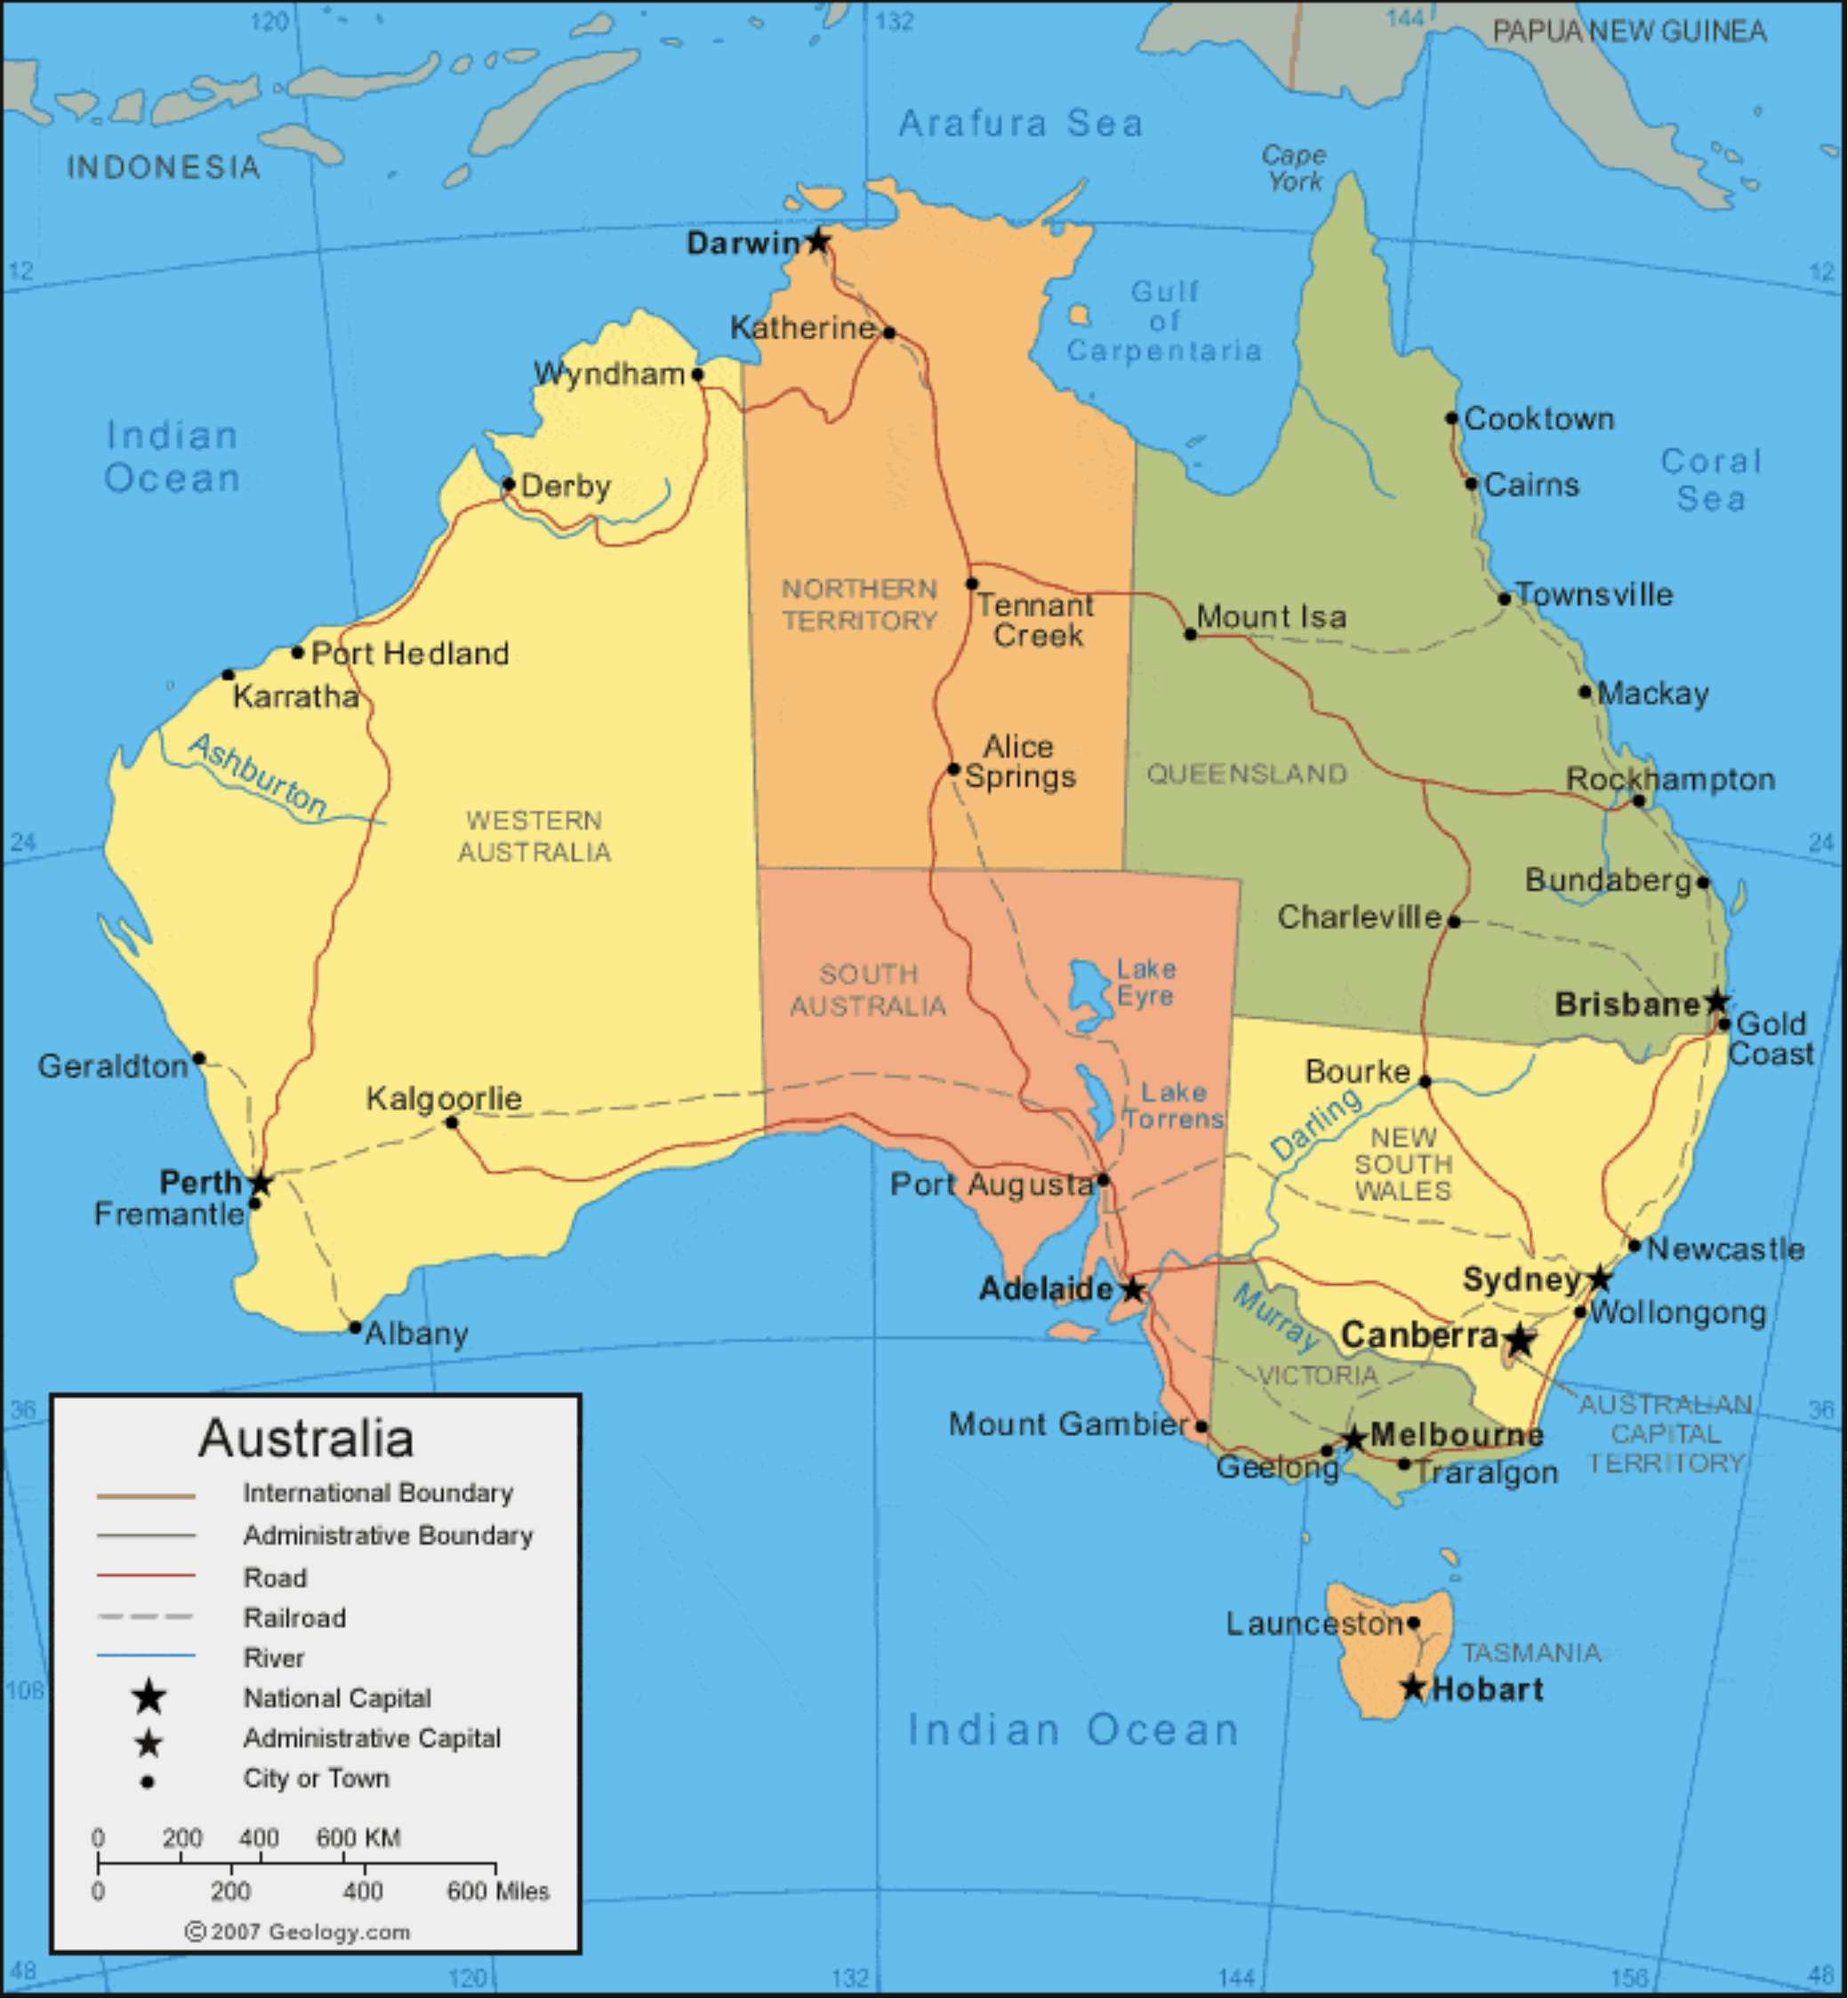
\epsfig{file=Figures/australia.pdf,scale=0.8}} 
  \caption{A map of Australia.}
  \label{fig:australia.pdf}
\end{figure}

\subsection{Example: Map Colouring}
In \href{https://en.wikipedia.org/wiki/Four_color_theorem}{map colouring} \index{map colouring} a map showing
different state 
borders is given and the task is to colour the different states such that no two states that have a common
border share the same colour.  \myFig{australia.pdf} shows a map of Australia.  There are seven different
states in Australia:
\begin{enumerate}
\item Western Australia, abbreviated as $\mathrm{WA}$,
\item Northern Territory, abbreviated as $\mathrm{NT}$,
\item South Australia, abbreviated as $\mathrm{SA}$,
\item Queensland, abbreviated as $\mathrm{Q}$,
\item New South Wales, abbreviated as $\mathrm{NSW}$,
\item Victoria, abbreviated as $\mathrm{V}$, and
\item Tasmania, abbreviated as $\mathrm{T}$.
\end{enumerate}
Figure \ref{fig:australia.pdf} would certainly look better if different states had been coloured with different
colours.  For the purpose of 
this example let us assume that we have only the three colours \red{red}, \puregreen{green}, and \blue{blue} 
available.  The question then is whether it is  
possible to colour the different states in a way that no two neighbouring states share the same colour.  This
problem can be formalized as a constraint satisfaction problem.  To this end we define:
\begin{enumerate}
\item $\mytt{Vars} := \{ \mathtt{WA}, \mathtt{NT}, \mathtt{SA}, \mathtt{Q}, \mathtt{NSW}, \mathtt{V}, \mathtt{T} \}$,
\item $\mytt{Values} := \{ \mytt{red}, \mytt{green}, \mytt{blue} \}$,
\item $\mytt{Constraints} := $ \\[0.1cm]
      \hspace*{1.3cm}
      $\bigl\{ \mathtt{WA} \not= \mathtt{NT}, \mathtt{WA} \not= \mathtt{SA},
                 \mathtt{NT} \not= \mathtt{SA}, \mathtt{NT} \not= \mathtt{Q},
                 \mathtt{SA} \not= \mathtt{Q},  \mathtt{SA} \not= \mathtt{NSW}, \mathtt{SA} \not= \mathtt{V}, 
                 \mathtt{Q}  \not= \mathtt{NSW},
                 \mathtt{NSW}\not= \mathtt{V}
       \bigr\}
       $.
       \\[0.1cm]
       The constraints do not mention the variable \texttt{T} for Tasmania, as Tasmania does not share a common
       border with any of the other states.
\end{enumerate}
Then $\mathcal{P} := \langle \mytt{Vars}, \mytt{Values}, \mytt{Constraints} \rangle$ is a constraint satisfaction problem.  
If we define the assignment $\mathcal{I}$ such that
\begin{enumerate}
\item $\mathcal{I}(\mathtt{WA}) = \mytt{red}$,
\item $\mathcal{I}(\mathtt{NT}) = \mytt{blue}$,
\item $\mathcal{I}(\mathtt{SA}) = \mytt{green}$,
\item $\mathcal{I}(\mathtt{Q}) = \mytt{red}$,
\item $\mathcal{I}(\mathtt{NSW}) = \mytt{blue}$,
\item $\mathcal{I}(\mathtt{V}) = \mytt{red}$,
\item $\mathcal{I}(\mathtt{T}) = \mytt{green}$,
\end{enumerate}
then you can check that the assignment $\mathcal{I}$ is indeed a solution to the constraint satisfaction problem $\mathcal{P}$.
Figure \ref{fig:australia-solution.png} on page \pageref{fig:australia-solution.png} shows this solution.

\begin{figure}[!ht]
  \centering
  \framebox{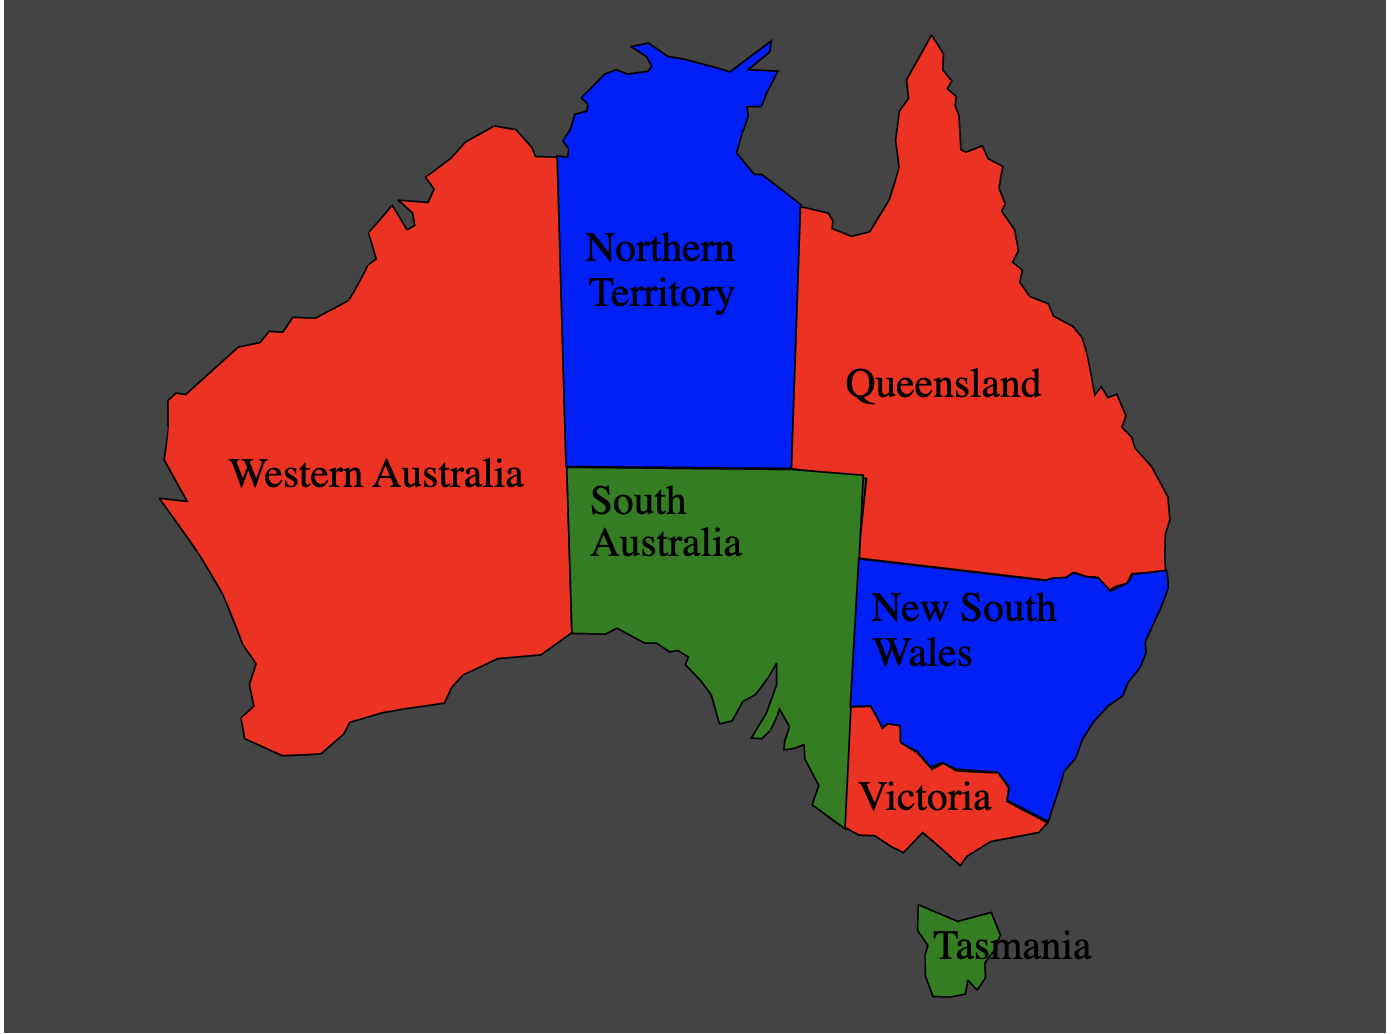
\epsfig{file=Figures/australia.png,scale=0.6}} 
  \caption{A map coloring for Australia.}
  \label{fig:australia-solution.png}
\end{figure}


\subsection{Example: The Eight Queens Puzzle}
\index{eight queens puzzle}
The \href{https://en.wikipedia.org/wiki/Eight_queens_puzzle}{eight queens problem} asks to put 8 queens onto a
chessboard such that no queen can attack another queen.  We have already discussed this problem in the previous
chapter.  Let us recapitulate: In \href{https://en.wikipedia.org/wiki/Chess}{chess},
a queen can attack all pieces that are either in the same row, the same column, or the same diagonal.  If we
want to put 8 queens on a chessboard such that no two queens can attack each other, we have to put exactly one
queen in every row:  If we would put more than one queen in a row, the queens in that row can attack each other.
If we would leave a row empty, then, given that the other rows contain at most one queen, there would be less
than 8 queens on the board.  Therefore, in order to model the eight queens problem as a constraint satisfaction
problem, we will use the following set of variables:
\\[0.2cm]
\hspace*{1.3cm}
$\mytt{Vars} := \{ \mytt{Q}_1, \mytt{Q}_2, \mytt{Q}_3, \mytt{Q}_4, \mytt{Q}_5, \mytt{Q}_6, \mytt{Q}_7,\mytt{Q}_8 \}$,
\\[0.2cm]
where for $i \in \{1,\cdots,8\}$ the variable $\mytt{Q}_i$ specifies the column of the queen that is placed in
row $i$.   As the columns run from one to eight, we define the set $\mytt{Values}$ as
\\[0.2cm]
\hspace*{1.3cm}
$\mytt{Values} := \{1,2,3,4,5,6,7,8\}$.
\\[0.2cm]
Next, let us define the constraints.  There are two different types of constraints.
\begin{enumerate}
\item We have constraints that express that no two queens positioned in different rows share the same column.
      To capture these constraints, we define
      \\[0.2cm]
      \hspace*{1.3cm}
      $\mytt{SameColumn} := \bigl\{ \mytt{Q}_i \not= \mytt{Q}_j \bigm| i \in \{1,\cdots,8\} \wedge j \in \{1,\cdots,8\} \wedge j < i \bigr\}$.
      \\[0.2cm]
      Here the condition $i < j$ ensures that, for example, we have the constraint $\mytt{Q}_2 \not= \mytt{Q}_1$
      but not the constraint  $\mytt{Q}_1 \not= \mytt{Q}_2$, as the latter constraint would be redundant if
      the former constraint has already been established.
\item We have constraints that express that no two queens positioned in different rows share the same 
      diagonal.  The queens in row $i$ and row $j$ share the same diagonal iff the equation
      \\[0.2cm]
      \hspace*{1.3cm}
      $|i - j| = |\mytt{Q}_i - \mytt{Q}_j|$
      \\[0.2cm]
      holds.  The expression $|i-j|$ is the absolute value of the difference of the rows of the queens in row
      $i$ and row $j$,  while the expression $|\mytt{Q}_i - \mytt{Q}_j|$ is the absolute value of the difference of the
      columns of these queens.  To capture these constraints, we define
      \\[0.2cm]
      \hspace*{1.3cm}
      $\mytt{SameDiagonal} := \bigl\{ |i  - j| \not= |\mytt{Q}_i - \mytt{Q}_j| \bigm| i \in \{1,\cdots,8\} \wedge j \in \{1,\cdots,8\} \wedge j < i \bigr\}$.
\end{enumerate}
Then, the set of constraints is defined as 
\\[0.2cm]
\hspace*{1.3cm}
$\mytt{Constraints} := \mytt{SameColumn} \cup \mytt{SameDiagonal}$
\\[0.2cm]
and the eight queens problem can be stated as the constraint satisfaction problem
\\[0.2cm]
\hspace*{1.3cm}
$\mathcal{P} := \langle \mytt{Vars}, \mytt{Values}, \mytt{Constraints} \rangle$.
\\[0.2cm]
If we define the assignment $\mathcal{I}$ such that
\\[0.2cm]
\hspace*{1.3cm}
$\mathcal{I}(\mytt{Q}_1) := 4,\; \mathcal{I}(\mytt{Q}_2) := 8,\; \mathcal{I}(\mytt{Q}_3) := 1,\;
\mathcal{I}(\mytt{Q}_4) := 2,\; \mathcal{I}(\mytt{Q}_5) := 6,\; \mathcal{I}(\mytt{Q}_6) := 2$,
\\[0.2cm]
\hspace*{1.3cm}
$\mathcal{I}(\mytt{Q}_7) := 7,\; \mathcal{I}(\mytt{Q}_8) := 5$,
\\[0.2cm]
then it is easy to see that this assignment is a solution of the eight queens problem.  This solution is shown
in \myFig{eight-queens.txt}.


\begin{figure}[!ht]
  \centering
\hspace*{0.0cm}
\vbox{\offinterlineskip
   \hrule height1pt
   \hbox{\vrule width1pt\bigchess
         \vbox{\hbox{0Z0L0Z0Z}
               \hbox{Z0Z0Z0ZQ}
               \hbox{QZ0Z0Z0Z}
               \hbox{Z0L0Z0Z0}
               \hbox{0Z0Z0L0Z}
               \hbox{ZQZ0Z0Z0}
               \hbox{0Z0Z0ZQZ}
               \hbox{Z0Z0L0Z0}}%
         \vrule width1pt}
   \hrule height1pt}

  \caption{A solution of the eight queens problem.}
  \label{fig:eight-queens.txt}
\end{figure}
Later, when we implement procedures to solve  \textsc{Csp}s, we will represent variable assignments and partial
variable assignments as dictionaries.  For example, the variable assignment $\mathcal{I}$ defined above would
then be represented as the dictionary 
\\[0.2cm]
\hspace*{1.3cm}
$\mathcal{I} = \bigl\{ \mytt{Q}_1:4,\, \mytt{Q}_2:8,\, \mytt{Q}_3:1,\, \mytt{Q}_4:3,\, 
             \mytt{Q}_5:6,\, \mytt{Q}_6:2,\, \mytt{Q}_7:7,\, \mytt{Q}_8:5) 
     \bigr\}$.
\\[0.2cm]
If we define 
\\[0.2cm]
\hspace*{1.3cm}
$\mathcal{B} := \bigl\{ \mytt{Q}_1:4,\, \mytt{Q}_2:8,\, \mytt{Q}_3:1) \bigr\}$,
\\[0.2cm]
then $\mathcal{B}$ is a partial assignment and $\mytt{dom}(\mathcal{B}) = \{ \mytt{Q}_1, \mytt{Q}_2, \mytt{Q}_3 \}$.  This
partial assignment is shown in \myFig{eight-queens-partial.txt}.

\begin{figure}[!ht]
  \centering
\hspace*{0.0cm}
\vbox{\offinterlineskip
   \hrule height1pt
   \hbox{\vrule width1pt\bigchess
         \vbox{\hbox{0Z0L0Z0Z}
               \hbox{Z0Z0Z0ZQ}
               \hbox{QZ0Z0Z0Z}
               \hbox{Z0Z0Z0Z0}
               \hbox{0Z0Z0Z0Z}
               \hbox{Z0Z0Z0Z0}
               \hbox{0Z0Z0Z0Z}
               \hbox{Z0Z0Z0Z0}}%
         \vrule width1pt}
   \hrule height1pt}

  \caption{The partial assignment $\bigl\{ \mytt{Q}_1 \mapsto 4, \mytt{Q}_2 \mapsto 8, \mytt{Q}_3 \mapsto 1) \bigr\}$.}
  \label{fig:eight-queens-partial.txt}
\end{figure}



\myFig{queens-csp.stlx} shows a \textsl{Python} program that can be used to create the eight queens puzzle as a
\textsc{Csp}.  

\begin{figure}[!ht]
\centering
\begin{minted}[ frame         = lines, 
                framesep      = 0.3cm, 
                firstnumber   = 1,
                bgcolor       = sepia,
                numbers       = left,
                numbersep     = 0.3cm,
                xleftmargin   = 0.2cm,
                xrightmargin  = 0.2cm,
              ]{python3}
 def queensCSP():
     'Returns a CSP coding the 8 queens problem.'
     S            = range(1, 8+1)          # used as indices
     Variables    = [ f'Q{i}' for i in S ]
     Values       = { 1, 2, 3, 4, 5, 6, 7, 8 }
     SameColumn   = { f'Q{i} != Q{j}' for i in S for j in S if i < j }
     SameDiagonal = { f'abs(Q{i}-Q{j}) != {j-i}' for i in S for j in S if i < j }
     return (Variables, Values, SameColumn | SameDiagonal)
\end{minted}
\vspace*{-0.3cm}
\caption{\textsl{Python} code to create the CSP representing the eight queens puzzle.}
\label{fig:queens-csp.stlx}
\end{figure}


\subsection{A Backtracking Constraint Solver}
One approach to solve a \textsc{Csp} that is both conceptually simple and reasonable efficient is
\blue{backtracking}.\index{backtracking}  The idea is to try to build variable assignments incrementally:  We start with
an empty dictionary and pick a variable $x_1$ that needs to have a value assigned.  For this variable, we
choose a value $v_1$ and assign it to this variable.  This yields the partial assignment $\{ x_1:v_1 \}$.
Next, we evaluate all those constraints that mention only the variable $x_1$ and check whether these constraints
are satisfied.  If any of these constraints is evaluated as \mytt{False}, we try to assign another value to
$x_1$ until we find a value that satisfies all constraints that mention only $x_1$.

In general, if we have a partial variable assignment $\mathcal{B}$ of the form
\\[0.2cm]
\hspace*{1.3cm}
$\mathcal{B} = \{ x_1:v_1, \cdots, x_k:v_k \}$
\\[0.2cm]
and we already know that all constraints that mention only the variables $x_1$, $\cdots$, $x_k$ are satisfied
by $\mathcal{B}$, then in order to extend $\mathcal{B}$ we pick another variable $x_{k+1}$ and choose a
value $v_{k+1}$ such that all those constraints that mention only the variables  $x_1$, $\cdots$, $x_k$,
$x_{k+1}$ are satisfied.  If we discover that there is no such value $v_{k+1}$, then we have to undo the
assignment $x_k:v_k$ and try to find a new value $v_k$ such that, first, those constraints mentioning only 
the variables  $x_1$, $\cdots$, $x_k$ are satisfied, and, second, it is possible to find a value $v_{k+1}$ that
can be assigned to $x_{k+1}$.  This step of going back and trying to find a new value for the variable $x_k$ is
called \blue{backtracking}.  It might be necessary to backtrack more than one level and to also undo the
assignment of $v_{k-1}$ to $x_{k-1}$ or, indeed, we might be forced to undo the assignments of all variables
$x_i$, $\cdots$, $x_k$ for some $i \in \{1,\cdots, n\}$.  The details of this search procedure are best
explained by looking at its implementation. \myFig{CSP-Solver.ipynb} shows a simple \textsc{Csp} solver that
employs backtracking.  We discuss this program next.

\begin{figure}[!ht]
\centering
\begin{minted}[ frame         = lines, 
                  framesep      = 0.3cm, 
                  firstnumber   = 1,
                  bgcolor       = sepia,
                  numbers       = left,
                  numbersep     = 0.3cm,
                  xleftmargin   = 0.8cm,
                  xrightmargin  = 0.8cm,
                  ]{python3}
import ast
              
def collect_variables(expr): 
    tree = ast.parse(expr)
    return { node.id for node in ast.walk(tree) 
                     if  isinstance(node, ast.Name) 
                     if  node.id not in dir(__builtins__)
           }
              
def solve(CSP):
    'Compute a solution for the given constraint satisfaction problem.'
    Variables, Values, Constraints = CSP
    CSP = (Variables,
           Values,
           [(f, collect_variables(f) & set(Variables)) for f in Constraints]
          )
    return backtrack_search({}, CSP)
\end{minted}
\vspace*{-0.3cm}
\caption{A backtracking \textsc{Csp} solver}
\label{fig:CSP-Solver.ipynb}
\end{figure}

\begin{enumerate}
\item As we need to determine the variables occurring in a given constraint, we import the module
      \mytt{ast}.  This module implements the function $\mytt{parse}(e)$ that takes
      a \textsl{Python} expression $e$.  This expression is parsed and the resulting syntax tree is returned.
\item The function $\mytt{collect\_variables}(\mytt{expr})$ takes a \textsl{Python} expression as its input.
      It returns the set of variable names occurring in this expression.

      The details of this implementation are quite technical and are not important in the following.
\item The procedure $\mytt{solve}$ takes a constraint satisfaction problem $\mytt{CSP}$ as input and tries
      to find a solution.    
      \begin{enumerate}
      \item First, in line 11 the $\mytt{CSP}$ is split into its three components.  However, the first
            component $\mytt{Variables}$ does not have to be a set but rather can also be a list.
            If $\mytt{Variables}$ is a list, then backtracking search will assign these variables 
            in the same order as they appear in this list.  This can improve the efficiency of backtracking
            tremendously. 
      \item Next, for every constraint $\mytt{f}$ of the given $\mytt{CSP}$, we compute the set of variables that
            are used in $\mytt{f}$.  This is done using the procedure $\mytt{collect\_variables}$.
            Of these variables we keep only those variables that also occur in the set $\mytt{Variables}$
            because we assume that any other \textsl{Python} variable occurring in a constraint $f$ has already
            a value assigned to it and can therefore be regarded as a constant.

            The variables occurring in a constraint $\mytt{f}$ are then paired with the constraint $\mytt{f}$ and
            the correspondingly modified data structure is stored in $\mytt{CSP}$ and is called an
            \blue{augmented \textsc{Csp}}.

            The reason to compute and store these sets of variables is efficiency: When we later check whether
            a constraint $\mytt{f}$ is satisfied for a partial variable assignment $\mytt{Assignment}$ where $\mytt{Assignment}$ is
            stored as a dictionary, we only need to check the constraint $\mytt{f}$ iff all of the variables occurring
            in $\mytt{f}$ are elements of the domain of $\mytt{Assignment}$.   It would be wasteful to compute
            these sets of all variables occurring in a given formula every time the formula is checked.
      \item Next, we call the function $\mytt{backtrack\_search}$ to compute a solution of $\mytt{CSP}$.
   \end{enumerate}
 \end{enumerate}

 \begin{figure}[!ht]
\centering
\begin{minted}[ frame         = lines, 
                  framesep      = 0.3cm, 
                  firstnumber   = 1,
                  bgcolor       = sepia,
                  numbers       = left,
                  numbersep     = 0.3cm,
                  xleftmargin   = 0.0cm,
                  xrightmargin  = 0.0cm,
                ]{python3}          
def backtrack_search(Assignment, CSP):
    '''
    Given a partial variable assignment, this function tries to 
    complete this assignment towards a solution of the CSP.
    '''
    Variables, Values, Constraints = CSP
    if len(Assignment) == len(Variables): 
        return Assignment
    var = [x for x in Variables if x not in Assignment][0]
    for value in Values:
        if isConsistent(var, value, Assignment, Constraints):
            NewAssign      = Assignment.copy()
            NewAssign[var] = value
            Solution = backtrack_search(NewAssign, CSP)
            if Solution != None:
                return Solution
    return None 
\end{minted}
\vspace*{-0.3cm}
\caption{The function \mytt{backtrack\_search}}
\label{fig:CSP-Solver.ipynb-backtrack_search}
\end{figure}

Next, we discuss the implementation of the procedure $\mytt{backtrack\_search}$ that is shown in
\myFig{CSP-Solver.ipynb-backtrack_search}.  This procedure receives a partial assignment 
$\mytt{Assignment}$ as input together with an augmented $\mytt{CSP}$.  This partial assignment is
\blue{consistent} with $\mytt{CSP}$:  If $\mytt{f}$ is a constraint of $\mytt{CSP}$ such that
all the variables occurring in $\mytt{f}$ are assigned to in $\mytt{Assignment}$, then evaluating
$\mytt{f}$ using $\mytt{Assignment}$ yields $\mytt{True}$.  Initially, this partial assignment is empty
and hence trivially consistent.  The idea is to extend this partial assignment until it is a complete
assignment that satisfies all constraints of the given $\mytt{CSP}$.
\begin{enumerate}
\item First, the augmented $\mytt{CSP}$ is split into its components.
\item Next, if $\mytt{Assignment}$ is already a complete variable assignment, i.e.~if the dictionary
      $\mytt{Assignment}$ has as many elements as there are variables, then the fact that
      $\mytt{Assignment}$ is partially consistent implies that
      it is a solution of the $\mytt{CSP}$ and, therefore, it is returned.
\item Otherwise, we have to extend the partial $\mytt{Assignment}$.  In order to do so, we first have to
      select a variable $\mytt{var}$ that has not yet been assigned a value in $\mytt{Assignment}$ so far.
      We pick the first variable in the list \mytt{Variables} that is yet unassigned.
      This variable is called $\mytt{var}$.
\item Next, we try to assign a $\mytt{value}$ to the selected variable $\mytt{var}$.  After assigning
      a $\mytt{value}$ to $\mytt{var}$, we immediately check whether this assignment would be consistent
      with the constraints using the procedure $\mytt{isConsistent}$.
      If the partial $\mytt{Assignment}$ turns out to be consistent, the partial $\mytt{Assignment}$
      is extended to the new partial assignment \mytt{NewAssign} that satisfies
      \\[0.2cm]
      \hspace*{1.3cm}
      \mytt{NewAssign[var] = value}
      \\[0.2cm]
      and that coincides with $\mytt{Assignment}$ for all variables different from $\mytt{var}$.
      Then, the procedure $\mytt{backtrack\_search}$ is called recursively to complete this new partial assignment.
      If this is successful, the resulting assignment is a solution of the CSP and is returned.  Otherwise the
      \texttt{for}-loop in line 10 tries the next $\mytt{value}$.
      If all possible values have been tried and none was successful, the \texttt{for}-loop
      ends and the function returns $\mytt{None}$.
\end{enumerate}


\begin{figure}[!ht]
\centering
\begin{minted}[ frame         = lines, 
                framesep      = 0.3cm, 
                firstnumber   = 1,
                bgcolor       = sepia,
                numbers       = left,
                numbersep     = -0.2cm,
                xleftmargin   = 0.0cm,
                xrightmargin  = 0.0cm,
              ]{python3}  
    def isConsistent(var, value, Assignment, Constraints):
        NewAssign      = Assignment.copy()
        NewAssign[var] = value
        return all(eval(f, NewAssign) for (f, Vs) in Constraints
                                      if var in Vs and Vs <= NewAssign.keys()
                  )
\end{minted}
\vspace*{-0.3cm}
\caption{The procedure \mytt{isConsistent}}
\label{fig:CSP-Solver.ipynb-isConsistent}
\end{figure}

We still need to discuss the implementation of the auxiliary procedure $\mytt{isConsistent}$
shown in \myFig{CSP-Solver.ipynb-isConsistent}.  This procedure takes a variable $\mytt{var}$, a $\mytt{value}$, a partial 
$\mytt{Assignment}$ and a set of $\mytt{Constraints}$.  It is assumed that $\mytt{Assignment}$ is
\blue{partially consistent} with respect to the set $\mytt{Constraints}$, i.e.~for every formula $\mytt{f}$
occurring in $\mytt{Constraints}$ such that
\\[0.2cm]
\hspace*{1.3cm}
$\mytt{vars}(\mytt{f}) \subseteq \mytt{dom}(\mytt{Assignment})$
\\[0.2cm]
holds, the formula $\mytt{f}$ evaluates to $\mytt{True}$ given the $\mytt{Assignment}$.  The purpose of
$\mytt{isConsistent}$ is to check, whether the extended assignment
\\[0.2cm]
\hspace*{1.3cm}
$\mytt{NewAssign} \;\mytt{:=}\;\mytt{Assignment} \cup \{ \pair(\mytt{var}, \mytt{value}) \}$
\\[0.2cm]
that assigns $\mytt{value}$ to the variable $\mytt{var}$ is still partially consistent with $\mytt{Constraints}$. 
To this end, the \mytt{for}-loop iterates over all $\mytt{Formula}$s in $\mytt{Constraints}$. 
However, we only have to check those $\mytt{Formula}$s that contain the variable $\mytt{var}$ and,
furthermore, have the property that
\\[0.2cm]
\hspace*{1.3cm}
$\mytt{Vars}(\mytt{Formula}) \subseteq \mytt{dom}(\mytt{NewAssign})$,
\\[0.2cm]
i.e.~all variables occurring in $\mytt{Formula}$ need to have a value assigned in
$\mytt{NewAssign}$.  The reasoning is as follows:
\begin{enumerate}
\item If $\mytt{var}$ does not occur in $\mytt{Formula}$, then adding $\mytt{var}$ to
      $\mytt{Assignment}$ cannot change the result of evaluating $\mytt{Formula}$ and as
      $\mytt{Assignment}$ is assumed to be partially consistent with respect to $\mytt{Formula}$, 
      $\mytt{NewAssign}$ is also partially consistent with respect to $\mytt{Formula}$.
\item If $\mytt{dom}(\mytt{NewAssign}) \not\subseteq \mytt{Vars}(\mytt{Formula})$, then $\mytt{Formula}$ can not be evaluated anyway. 
\end{enumerate}
If we use backtracking, we can solve the 8 queens puzzle in less than a second.
For the 8 queens puzzle the order in which variables are tried is not particularly important.  The reason
is that all variables are connected to all other variables.  For other problems the ordering of the variables
can be \red{very important}.  The general strategy is that variables that are strongly related to each other should
be grouped together in the list $\mytt{Variables}$.

\exerciseEng
We have already discussed the \href{https://en.wikipedia.org/wiki/Zebra_puzzle}{Zebra Puzzle} in section
\ref{section:zebra} of the previous chapter.  Your task is to reformulate this puzzle as a constraint
programming problem.  You should start from the following notebook:
\\[0.2cm]
\hspace*{1.3cm}
\href{https://github.com/karlstroetmann/Logic/blob/master/Python/Chapter-4/Prince-Tiger.ipynb}{\texttt{github.com/karlstroetmann/Logic/blob/master/Python/Chapter-5/Zebra-CSP.ipynb}}
\\[0.2cm]
While it is important to order the variables in a sensible way, you shouldn't spend to much time with this
task.
\eox

\exerciseEng
Figure \ref{fig:send-more-money.pdf} shows a
\href{https://en.wikipedia.org/wiki/Verbal_arithmetic}{cryptarithmetic puzzle}.
The idea is that the letters 
``$\texttt{S}$'', ``$\texttt{E}$'', ``$\texttt{N}$'', ``$\texttt{D}$'', ``$\texttt{M}$'', ``$\texttt{O}$'', ``$\texttt{R}$'', ``$\texttt{Y}$'' 
are interpreted as variables ranging over the set of decimal digits, i.e.~these variables can take values in
the set $\{0,1,2,3,4,5,6,7,8,9\}$.  Then, the string ``$\texttt{SEND}$'' is interpreted as a decimal number,
i.e.~it is interpreted as the number
\\[0.2cm]
\hspace*{1.3cm}
$\texttt{S} \cdot 10^3 + \texttt{E} \cdot 10^2 + \texttt{N} \cdot 10^1 + \texttt{D} \cdot 10^0$.
\\[0.2cm]
The strings ``$\texttt{MORE}$ and ``$\texttt{MONEY}$'' are interpreted similarly. To make the problem
interesting, the assumption is that different variables have different values.  Furthermore, the
digits at the beginning of a number should be different from $0$.


\begin{figure}[!ht]
\centering
\framebox{
\epsfig{file=Figures/send-more-money.pdf, scale=0.4}}

\caption{A cryptarithmetic puzzle}
\label{fig:send-more-money.pdf}
\end{figure}

Your task is to reformulate this puzzle as a constraint
programming problem.  You should start from the following notebook:
\\[0.2cm]
\hspace*{0.3cm}
\href{https://github.com/karlstroetmann/Logic/blob/master/Python/Chapter-5/Crypto-Arithmetic.ipynb}{\texttt{github.com/karlstroetmann/Logic/blob/master/Python/Chapter-5/Crypto-Arithmetic.ipynb}}
\\[0.2cm]
It is importtant that you add the digits one by one as in elementary school.  This way, the addition is
separated into a number of constraints that can then be solved by backtracking.  \eox

\section{Solving Search Problems by Constraint Programming}
In this section we show how we can formulate certain \blue{search problems} as \mytt{CSP}s.
We will explain our method by solving the
\href{https://en.wikipedia.org/wiki/Missionaries_and_cannibals_problem}{missionaries and cannibals problem},
which is explained in the following:
Three missionaries and three infidels have to cross a river in order to get to a church where the infidels can
be baptized.  According to ancient catholic mythology, baptizing the infidels is necessary to save them from
the eternal tortures of hell fire. In order to cross the river, the missionaries and infidels have a small boat
available that can take at most two passengers. If at any moments at any shore there are more infidels than
missionaries, then the missionaries have a problem, since the infidels have a diet that is rather unhealthy for
the missionaries. 

In order to solve this problem via constraint programming, we first introduce the notion of a
\blue{symbolic transition system}.

\begin{Definition}[Symbolic Transition System]
  A symbolic transition system is a 6-tuple
  \\[0.2cm]
  \hspace*{1.3cm}
  $\mathcal{T} = \langle \mathtt{Vars}, \mathtt{Values}, \mathtt{Start}, \mathtt{Goal}, \mathtt{Invariant}, \mathtt{Transition} \rangle$
  \\[0.2cm]
  such that:
  \begin{enumerate}[(a)]
  \item \texttt{Vars} is a set of variables.

        These variables are strings.  For every variable $x \in \texttt{Vars}$ there is a \blue{primed}
        variable $x'$ which does not occur in \texttt{Vars}.  The set of these primed Variables is denoted as
        $\mathtt{Vars}'$.
  \item \texttt{Values} is a set of values that these variables can take.
  \item \texttt{Start}, \texttt{Goal}, and \texttt{Invariant} are first-order formulas such that all free
         variables occurring in these formulas are elements from the set \texttt{Vars}.
         \begin{itemize}
         \item \texttt{Start} describes the initial state of the transition system.
         \item \texttt{Goal} describes a state that should be reached by the transition system.
         \item \texttt{Invariant} is a formula that has to be true for every state of the transition system.
         \end{itemize}
  \item \texttt{Transition} is a first-order formula.  The free variables of this formula are elements of
        the set $\texttt{Vars} \cup \mathtt{Vars}'$, i.e.~they are either variables from the set \texttt{Vars}
        or they are primed variables from the set $\mathtt{Vars}'$.

        The formula \texttt{Transition} describes how the variables in the transition system change during a
        state transition.  The primed variables refer to the values of the original variables after the
        state transition.
  \end{enumerate}
\end{Definition}
Every \blue{state} of a transition system is a mapping of the variable to values.
The idea is that the formula \texttt{Start} describes the start state of our search problem, \texttt{Goal}
describes the state that we want to reach, while \texttt{Invariant} is a formula that must be true initially
and that has to remain true after every transition of our system.


In order to clarify this definition we show how the \emph{missionaries and cannibals} problem can be formulated as
a symbolic transition system.
\begin{enumerate}[(a)]
\item $\texttt{Vars} := \{ \mathtt{M}, \mathtt{C}, \mathtt{B} \}$.

      The value of \texttt{M} is the number of missionaries on the western shore, the value of \texttt{C} is
      the number of infidels on that shore, while the value of \texttt{B} is the number of boats on the western
      shore.
\item $\mathtt{Values} := \{ 0, 1, 2, 3 \}$.
\item $\texttt{Start} := (\mathtt{M} = 3 \wedge \mathtt{C} = 3 \wedge \mathtt{B} = 1)$.
\item $\texttt{Goal}  := (\mathtt{M} = 0 \wedge \mathtt{C} = 0 \wedge B = 0)$.
\item $\texttt{Invariant} := \bigl((\mathtt{M} = 3 \vee \mathtt{M} = 0 \vee \mathtt{M} = \mathtt{C}) \;\wedge\; \mathtt{B} \leq 1\bigr)$.

      The first part of the invariant, i.e.~ the formulas $\mathtt{M} = 3 \vee \mathtt{M} = 0 \vee \mathtt{M} = \mathtt{C}$,
      describes those states where the missionaries are not threatened by the infidels.
      \begin{itemize}
      \item $\mathtt{M} = 3$: All missionaries are on the western shore.
      \item $\mathtt{M} = 0$: All missionaries are together on the eastern shore.
      \item $\mathtt{M} = \mathtt{C}$: On both shores the numbers of missionaries and cannibals are the same.

            If neither $\mathtt{M} = 3$ nor $\mathtt{M} = 0$ holds, then the number of missionaries and
            cannibals have to be the same on the western shorem because if there were more missionaries on the
            western shore than cannibals, then there would be less missionaries than cannibals on the eastern
            shore and hence there would be a problem on the eastern shore.
      \end{itemize}
      The condition $\mathtt{B} \leq 1$ has to be true because there is just one boat.
\item $\texttt{Transition} :=
      \begin{array}[t]{cl}
         &  \mathtt{B}' = 1 - \mathtt{B}   \\[0.2cm]
        \wedge & \bigl(\mathtt{B} = 1 \;\rightarrow\; 1 \leq \mathtt{M} - \mathtt{M}'  + \mathtt{C} - \mathtt{C}' \leq 2 \;\wedge\;
        \mathtt{M}' \leq \mathtt{M} \;\wedge\; \mathtt{C}' \leq \mathtt{C}\bigr) \\[0.2cm]
        \wedge & \bigl(\mathtt{B} = 0 \;\rightarrow\; 1 \leq \mathtt{M}' - \mathtt{M}  + \mathtt{C}' - \mathtt{C} \leq 2 \;\wedge\;
                \mathtt{M}' \geq \mathtt{M} \;\wedge\; \mathtt{C}' \geq \mathtt{C}\bigr) 
      \end{array}
      $

      Let us explain the details of this formula:
      \begin{itemize}
      \item $\mathtt{B}' = 1 - \mathtt{B}$

            If the boat is initially on the western shore, i.e. $\texttt{B} = 1$, it will be on the eastern
            shore afterwards, i.e. we will then have $\texttt{B}' = 0$.  If, instead, the boat is initially on
            the eastern shore, i.e. $\texttt{B} = 0$, it will be on the western
            shore afterwards and then we have $\texttt{B}' = 1$.
      \item $\mathtt{B} = 1 \;\rightarrow\; 1 \leq \mathtt{M} - \mathtt{M}'  + \mathtt{C} - \mathtt{C}' \leq 2 \;\wedge\;
             \mathtt{M}' \leq \mathtt{M} \;\wedge\; \mathtt{C}' \leq \mathtt{C}$


            If the boat is initially on the western shore, then afterwards the number of missionaries and
            infidels will decrease, as they leave for the eastern shore.  In this case $\texttt{M} - \texttt{M}'$
            is the number of missionaries on the boat, while $\texttt{C} - \texttt{C}'$ is the number of
            infidels.  The sum of these numbers has to be between $1$ and $2$ because the boat can not travel
            empty and can take at most two passengers.

            The condition $\mathtt{M}' \leq \mathtt{M}$ is true because when missionaries are traveling from
            the western shore to the eastern shore, the number of missionaries on the western shore can not
            increase.  Similarly,  $\mathtt{C}' \leq \mathtt{C}$ has to be true.
      \item $\mathtt{B} = 0 \;\rightarrow\; 1 \leq \mathtt{M}' - \mathtt{M}  + \mathtt{C}' - \mathtt{C} \leq 2 \;\wedge\;
            \mathtt{M}' \geq \mathtt{M} \;\wedge\; \mathtt{C}' \geq \mathtt{C}$

            This formula describes the transition from the eastern shore to the western shore and is analogous
            to the previous formula.
      \end{itemize}
\end{enumerate}


\begin{figure}[!ht]
\centering
\begin{Verbatim}[frame         = single, 
                 framesep      = 0.3cm,
                 framerule=0.5mm,
                 rulecolor=\color{black},
                 firstnumber   = 1,
                 numbers       = left,
                 numbersep     = 0.3cm,
                 xleftmargin   = 0.8cm,
                 xrightmargin  = 0.8cm,
                 commandchars  = \\\{\},
                 codes         = {\catcode`$=3\catcode`^=7}
               ] 
\colorbox{sepia}{def start(M, C, B):                                                       }
\colorbox{sepia}{    return M == 3 and C == 3 and B == 1                                   }
\colorbox{sepia}{                                                                          }
\colorbox{sepia}{def goal(M, C, B):                                                        }
\colorbox{sepia}{    return M == 0 and C == 0 and B == 0                                   }
\colorbox{sepia}{                                                                          }
\colorbox{sepia}{def invariant(M, C, B):                                                   }
\colorbox{sepia}{    return (M == 0 or M == 3 or M == C) and B <= 1                        }
\colorbox{sepia}{                                                                          }
\colorbox{sepia}{def transition(M$\alpha$, C$\alpha$, B$\alpha$, M$\beta$, C$\beta$, B$\beta$):                                   }
\colorbox{sepia}{    if not (B$\beta$ == 1 - B$\alpha$):                                                }
\colorbox{sepia}{        return False                                                      }
\colorbox{sepia}{    if B$\alpha$ == 1:                                                           }
\colorbox{sepia}{        return 1 <= M$\alpha$ - M$\beta$ + C$\alpha$ - C$\beta$ <= 2 and M$\beta$ <= M$\alpha$ and C$\beta$ <= C$\alpha$     }
\colorbox{sepia}{    else:                                                                 }
\colorbox{sepia}{        return 1 <= M$\beta$ - M$\alpha$ + C$\beta$ - C$\alpha$ <= 2 and M$\beta$ >= M$\alpha$ and C$\beta$ >= C$\alpha$     }
\end{Verbatim}
\vspace*{-0.3cm}
\caption{Coding the \emph{missionaries and cannibals problem} as a symbolic transition system.}
\label{fig:Missionaries-STS.ipynb}
\end{figure}

%$
Figure \ref{fig:Missionaries-STS.ipynb} shows how the \emph{missionaries and cannibals problem} can be
represented as a symbolic transition system in \textsl{Python}.  In the function \texttt{transition} 
we use the following convention: Since variables cannot be primed in
\textsl{Python} we append the character $\alpha$ to the names of the original
variables from the set \texttt{Vars}, while we append $\beta$ to these names to get the primed versions of the
corresponding variable.


\begin{figure}[!ht]
\centering
\begin{minted}[ frame         = lines, 
                framesep      = 0.3cm, 
                firstnumber   = 1,
                bgcolor       = sepia,
                numbers       = left,
                numbersep     = -0.2cm,
                xleftmargin   = 0.0cm,
                xrightmargin  = 0.0cm,
              ]{python3}
    def flatten(LoL):
        return [x for L in LoL for x in L]
                    
    def missionaries_CSP(n):
        "Returns a CSP encoding the problem."
        Lists        = [[f'M{i}', f'C{i}', f'B{i}'] for i in range(n+1)]
        Variables    = flatten(Lists)
        Values       = { 0, 1, 2, 3 }
        Constraints  = {  'start(M0, C0, B0)'      }  # start state
        Constraints |= { f'goal(M{n}, C{n}, B{n})' }  # goal state
        for i in range(n):
            Constraints.add(f'invariant(M{i}, C{i}, B{i})')
            Constraints.add(f'transition(M{i}, C{i}, B{i}, M{i+1}, C{i+1}, B{i+1})')
        return Variables, Values, Constraints
        
    def find_solution():
        n = 1
        while True:
            print(n)
            CSP = missionaries_CSP(n)
            Solution = solve(CSP)
            if Solution != None:
                return n, Solution
            n += 2
\end{minted}
\vspace*{-0.3cm}
\caption{Turning the symbolic transition system into a \textsc{Csp}.}
\label{fig:Missionaries-STS.ipynb-2}
\end{figure}

Figure \ref{fig:Missionaries-STS.ipynb-2} shows how we can turn the symbolic transition system into a
\textsc{Csp}.
\begin{enumerate}
\item The function $\texttt{flatten}(\texttt{LoL})$ receives a list of lists $\texttt{LoL}$ as its argument.
       This list has the form
       \\[0.2cm]
       \hspace*{1.3cm}
       $\texttt{LoL} = [L_1, \cdots, L_k]$
       \\[0.2cm]
       where the $L_i$ are lists for $i=1,\cdots,k$.
       
       It returns the list
       \\[0.2cm]
       \hspace*{1.3cm}
       $L_1 + \cdots + L_k$,
       \\[0.2cm]
       i.e.~it appends these lists and returns the result.
\item The function $\mathtt{missionaries\_CSP}(n)$ receives a natural number $n$ as its argument.
       It returns a \textsc{Csp} that has a solution if there is a solution of the \emph{missionaries and cannibals}
       problem that crosses the river exactly $n$ times.  It uses the variables
       \\[0.2cm]
       \hspace*{1.3cm}
       $\mathtt{M}_i$, $\mathtt{C}_i$, and $\mathtt{B}_i$, where $i=0,\cdots,n$.
       \\[0.2cm]
       $\mathtt{M}_i$ is the number of missionaries on the western shore after the boat has crossed the river
       $i$ times. The variables $\mathtt{C}_i$ and $\texttt{B}_i$ denote the number of infidels and boats
       respectively.

       Line 12 ensures that the invariant of the transition system is valid after every crossing of the boat.
       Line 13 describes the mechanics of the crossing.
\item The function \texttt{find\_solution} tries to find a natural number $n$ such that problem can be solved
       with $n$ crossings. As the number of crossings has to be odd, we increment $n$ by
       two at the end of the \texttt{while} loop.

       The function \texttt{find\_solution} needs less than 2 seconds to finc the solution.
\end{enumerate}
\pagebreak

\exerciseEng
An agricultural economist has to sell a \blue{wolf}, a \blue{goat}, and a \blue{cabbage}
on a market place.  In order to reach the market place, she has to cross a river.  The
boat that she can use is so small that it can only accommodate either the goat, the wolf,
or the cabbage in addition to the agricultural economist herself.  Now if the agricultural
economist leaves the wolf alone with the goat, the wolf will eat the goat.  If, instead,
the agricultural economist leaves the goat with the cabbage, the goat will eat the
cabbage.  Is it possible for the agricultural economist to develop a schedule that allows
her to cross the river without either the goat or the cabbage being eaten?

Encode this problem as a \blue{symbolic transition system} and then solve it with the help
of the constraints solver developed earlier.  Assume that the
problem can be solved with $n\in\mathbb{N}$ crossing of the river.  Use the following
variables:
\begin{itemize}
\item $\texttt{F}i$ for $i\in\{0,\cdots,n\}$ is the number of farmers on the western shore after the 
      $i^{\textrm{th}}$ crossing.
\item $\texttt{W}i$ for $i\in\{0,\cdots,n\}$ is the number of wolves on the western shore after the 
      $i^{\textrm{th}}$ crossing.
\item $\texttt{G}i$ for $i\in\{0,\cdots,n\}$ is the number of goats on the western shore after the 
      $i^{\textrm{th}}$ crossing.
\item $\texttt{C}i$ for $i\in\{0,\cdots,n\}$ is the number of cabbages on the western shore after the 
      $i^{\textrm{th}}$ crossing.
\end{itemize}
You should start from the following notebook:
\\[0.2cm]
\hspace*{-0.5cm}
\href{https://github.com/karlstroetmann/Logic/blob/master/Python/Chapter-5/Wolf-Goat-Cabbage-STS.ipynb}{\texttt{github.com/karlstroetmann/Logic/blob/master/Python/Chapter-5/Wolf-Goat-Cabbage-STS.ipynb}}
\eox
s
\section{The Z3 Solver}
We conclude this chapter with a discussion of the solver
\href{https://www.microsoft.com/en-us/research/project/z3-3/}{Z3}, which has beed developd
at Microsoft.  Z3 implements most of the state-of-the-art constraint solving algorithms
and is exceptionally powerful.  We introduce Z3 via a series of examples.

\subsection{A Simple Text Problem}
The following is a simple text problem from my old $8^{\textrm{th}}$ grade math book.
\textsl{
  \begin{itemize}
  \item I have as many brothers as I have sisters.
  \item My sister has twice as many brothers as she has sisters.
  \item How many children does my father have?
  \end{itemize}}
\noindent
In order to solve this puzzle we need two additional assumptions.
\begin{enumerate}
\item My father has no illegitimate children.
\item All of my fathers children identify themselves as either male or female.
\end{enumerate}
Strangely, in my old math book these assumptions have not been mentioned.

We can now infer the number of children.
If we denote the number of \blue{boys} by the variable $b$ and the number of \blue{girls}
by the variable $g$, the problem statements are equivalent to the following equations:
\begin{itemize}
\item $b - 1 = g$.
\item $2 \cdot (g - 1) = b$.
\end{itemize}
Before we can start to solve this problem, we have to install \texttt{Z3} via \texttt{pip} using the following
command:  
\\[0.2cm]
\hspace*{1.3cm}
\texttt{pip install z3-solver}


\begin{figure}[!ht]
\centering
\begin{minted}[ frame         = lines, 
                 framesep      = 0.3cm, 
                 firstnumber   = 1,
                 bgcolor       = sepia,
                 numbers       = left,
                 numbersep     = -0.2cm,
                 xleftmargin   = 0.8cm,
                 xrightmargin  = 0.8cm,
               ]{python3}             
    import z3
    
    boys  = z3.Int('boys')
    girls = z3.Int('girls')
    
    S = z3.Solver()
    
    S.add(boys - 1 == girls)
    S.add(2 * (girls - 1) == boys)
    S.check()
    Solution = S.model()
    
    b = Solution[boys ].as_long()
    g = Solution[girls].as_long()
    
    print(f'My father has {b + g} children.')
\end{minted}
\vspace*{-0.3cm}
\caption{Solving a simple text problem.}
\label{fig:Brothers-and-Sisters.ipynb}
\end{figure}

\noindent
Figure \ref{fig:Brothers-and-Sisters.ipynb} on page \pageref{fig:Brothers-and-Sisters.ipynb} shows how we can
solve the given problem using the \textsl{Python}
interface of Z3.
\begin{enumerate}
\item In line 1 we import the module \texttt{z3} so that we can use the Python \textsc{Api} of Z3.
      The documentation of this \textsc{Api} is available at the following address:
      \\[0.2cm]
      \hspace*{1.3cm}
      \href{https://ericpony.github.io/z3py-tutorial/guide-examples.htm}{https://ericpony.github.io/z3py-tutorial/guide-examples.htm}
\item Lines 3 and 4 creates the \texttt{Z3} variables \mytt{boys} and \mytt{girls} as integer valued variables.
      The function \mytt{Int} takes one argument, which has to be a string.  This string is the name of the
      variable.  We store these variables in Python variables of the same name.  It would be possible to use
      different names for the Python variables, but that would be very confusing.
\item Line 6 creates an object of the class \texttt{Solver}.  This is the constraint solver provided by
      \texttt{Z3}.
\item Lines 8 and 9 add the constraints expressing that the number of girls is one less than the number of boys
      and that my sister has twice as many brothers as she has sisters as constraints to the solver
      \texttt{S}.
\item In line 10 the method \mytt{check} examines whether the given set of constraints is satisfiable.
      In general, this method returns one of the following results:
      \begin{enumerate}[(a)]
      \item \mytt{sat} is returned if the problem is solvable, (\mytt{sat} is short for \emph{satisfiable})
      \item \mytt{unsat} is returned if the problem is unsolvable,
      \item \mytt{unknown} is returned if \texttt{Z3} is not powerful enough to solve the given problem.
      \end{enumerate}
\item Since in our case the method \mytt{check} returns \texttt{sat}, we can extract the solution that is
      computed via the method \mytt{model} in line 11.  
\item In order to extract the values that have been computed by \texttt{Z3} for the variables \mytt{boys} and
      \mytt{girls}, we can use dictionary syntax and write \mytt{Solution[boys]} and
      \mytt{Solution[girls]} to extract these values.  However, these values are not stored as integers but
      rather as objects of the class \mytt{IntNumRef}, which is some internal class of \texttt{Z3} to store
      integers.  This class provides the method \mytt{as\_long} that converts its argument into an integer number.
\end{enumerate}
\pagebreak

\exerciseEng
Solve the following text problem using \texttt{Z3}.
\textsl{
  \begin{enumerate}[(a)]
  \item A Japanese deli offers both
        \href{https://www.discovermagazine.com/health/hearty-penguin-steaks-the-old-school-explorers-salve-for-scurvy}{penguins}
        and \href{http://fancytoast.blogspot.com/2007/04/parrot-three-ways.html}{parrots}.  
  \item A parrot and a penguin together cost 666 bucks.
  \item The penguin costs 600 bucks more than the parrot.  
  \end{enumerate}}
  \noindent
  \textbf{What is the price of the parrot?} You may assume that the prizes of these
  delicacies are integer valued.
  You should start from the following notebook:
\\[0.2cm]
\hspace*{0.0cm}
\href{https://github.com/karlstroetmann/Logic/blob/master/Python/Chapter-5/Parrot-and-Penguin.ipynb}{\texttt{github.com/karlstroetmann/Logic/blob/master/Python/Chapter-5/Parrot-and-Penguin.ipynb}}
\eox

\exerciseEng
Solve the following text problem using \texttt{Z3}.
\textsl{
  \begin{enumerate}[(a)]
  \item  A train travels at a uniform speed for 360 miles.  
  \item  The train would have taken 48 minutes less to travel the same distance 
         if it had been faster by 5 miles per hour.
  \end{enumerate}}
\noindent
\textbf{Find the speed of the train!}

\noindent
\textbf{Hints:}
\begin{enumerate}[(a)]
\item As the speed is a real number you should declare this variable via the \texttt{Z3} function \texttt{Real} instead of using
      the function \texttt{Int}.
\item Be careful to not mix up different units. In particular, the time 48 minutes should be expressed as a
      fraction of an hour.
\item When you formulate the information given above, you will get a system of \textbf{non-linear} equations,
      which is equivalent to a quadratic equation.  This quadratic equation has two different solutions.
      One of these solutions is negative.  In order to exclude the negative solution you need to add a
      constraint stating that the speed of the train has to be greater than zero.
\end{enumerate}
You should start from the following notebook:
\\[0.2cm]
\hspace*{0.8cm}
\href{https://github.com/karlstroetmann/Logic/blob/master/Python/Chapter-5/Train-Z3.ipynb}{\texttt{github.com/karlstroetmann/Logic/blob/master/Python/Chapter-5/Train-Z3.ipynb}}
\eox

\subsection{The Knight's Tour}
In this subsection we will solve the puzzle \href{https://en.wikipedia.org/wiki/Knight%27s_tour}{The Knight's Tour} 
using \texttt{Z3}.  This puzzle asks whether it is possible for a knight to visit all 64 squares of a chess board
in 63 moves.  We will start the tour in the upper left corner of the board.  

In order to model this puzzle as a constraint satisfaction problem we first have to decide on the variables
that we want to use. The idea is to have 64 variables that describe the position of the knight after its
$i^{\mathrm{th}}$ move where $i=0,1,\cdots,63$.  However, it turns out that it is best to split the values of these positions up into a
row and a column.  If we do this, we end up with 128 variables of the form
\\[0.2cm]
\hspace*{1.3cm}
$\mathtt{R}_i$ and $\mathtt{C}_i$ \quad for $i \in \{0, 1, \cdots, 63\}$.
\\[0.2cm]
Here $\mathtt{R}_i$ denotes the row of the knight after its $i^{\mathrm{th}}$ move, while $\mathtt{C}_i$
denotes the corresponding column.  
Next, we have to formulate the constraints.  In this case, there are two kinds of constraints:
\begin{enumerate}
\item We have to specify that the move from the position $\langle \mathtt{R}_i, \mathtt{C}_i \rangle$
      to the position $\langle \mathtt{R}_{i+1}, \mathtt{C}_{i+1} \rangle$ is legal move for a knight.
      In chess, there are two ways for a knight to move:
      \begin{enumerate}[(a)]
      \item The knight can move two squares horizontally left or right followed by moving vertically
            one square up or down, or
      \item the knight can move two squares vertically up or down followed by moving
            one square left or right.
      \end{enumerate}
      Figure \ref{fig:knight-moves.png} shows all legal moves of a knight that is positioned in the square \texttt{e4}.
      Therefore, a formula that expresses that the $i^{\mathrm{th}}$ move is a legal move of the knight is a disjunction
      of the following eight formulas that each describe one possible way for the knight to move:
      \begin{enumerate}
      \item $\mathtt{R}_{i+1} = \mathtt{R}_{i} + 2 \;\wedge\; \mathtt{C}_{i+1} = \mathtt{C}_{i} + 1$,
      \item $\mathtt{R}_{i+1} = \mathtt{R}_{i} + 2 \;\wedge\; \mathtt{C}_{i+1} = \mathtt{C}_{i} - 1$, 
      \item $\mathtt{R}_{i+1} = \mathtt{R}_{i} - 2 \;\wedge\; \mathtt{C}_{i+1} = \mathtt{C}_{i} + 1$, 
      \item $\mathtt{R}_{i+1} = \mathtt{R}_{i} - 2 \;\wedge\; \mathtt{C}_{i+1} = \mathtt{C}_{i} - 1$, 
      \item $\mathtt{R}_{i+1} = \mathtt{R}_{i} + 1 \;\wedge\; \mathtt{C}_{i+1} = \mathtt{C}_{i} + 2$, 
      \item $\mathtt{R}_{i+1} = \mathtt{R}_{i} + 1 \;\wedge\; \mathtt{C}_{i+1} = \mathtt{C}_{i} - 2$, 
      \item $\mathtt{R}_{i+1} = \mathtt{R}_{i} - 1 \;\wedge\; \mathtt{C}_{i+1} = \mathtt{C}_{i} + 2$, 
      \item $\mathtt{R}_{i+1} = \mathtt{R}_{i} - 1 \;\wedge\; \mathtt{C}_{i+1} = \mathtt{C}_{i} - 2$. 
      \end{enumerate}
\item Furthermore, we have to specify that the position  $\langle \mathtt{R}_i, \mathtt{C}_i \rangle$ is
      different from the position  $\langle \mathtt{R}_j, \mathtt{C}_j \rangle$ if $i \not= j$.
\end{enumerate}


\begin{figure}[!ht]
  \centering
  \framebox{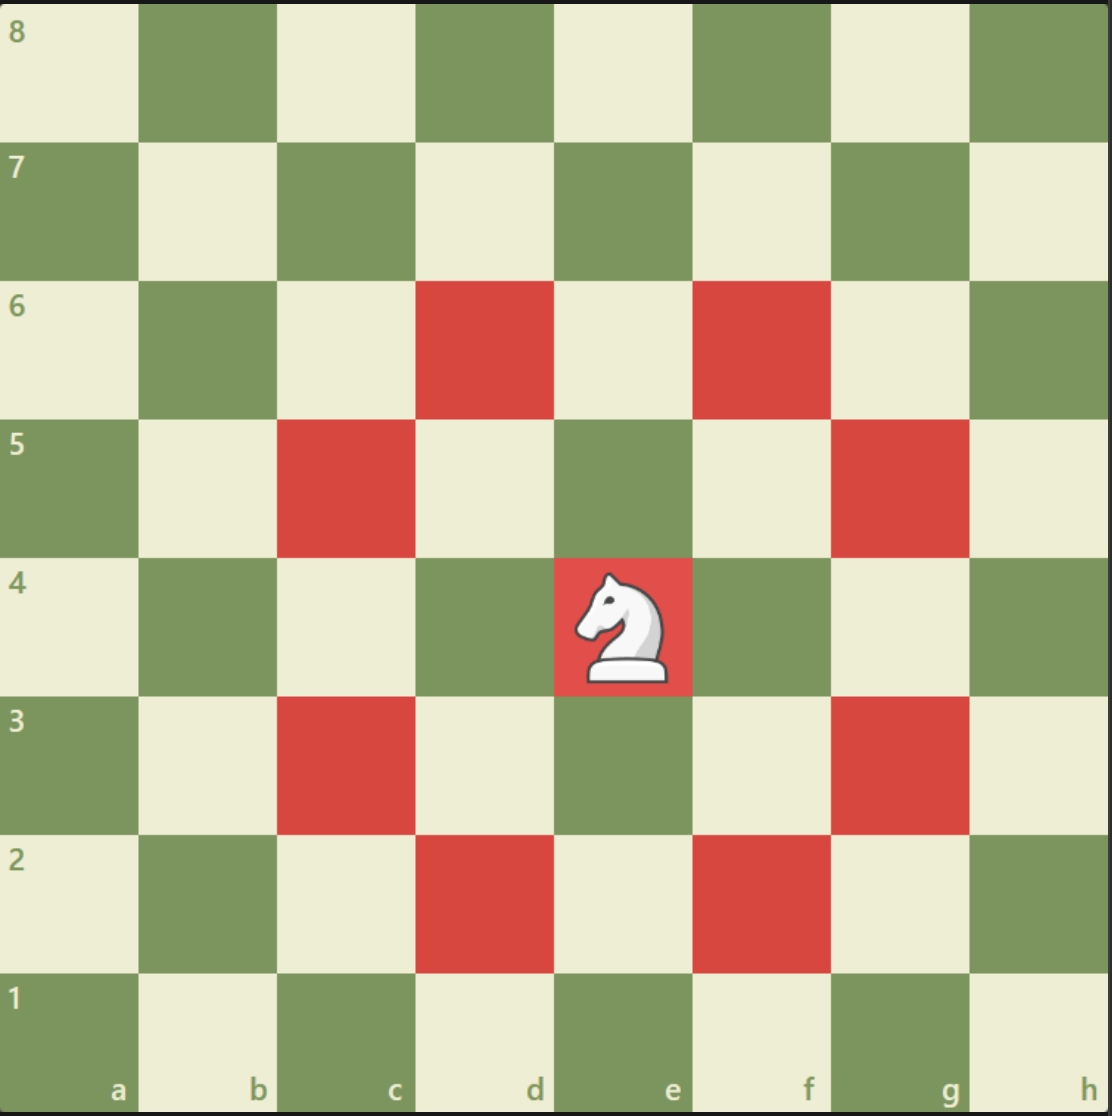
\epsfig{file=Figures/knight-moves.png, scale=0.5}} 
  \caption{The moves of a knight, courtesy of \href{https://www.chess.com/}{chess.com}.}
  \label{fig:knight-moves.png}
\end{figure}

\begin{figure}[!ht]
\centering
\begin{minted}[ frame         = lines, 
                 framesep      = 0.3cm, 
                 firstnumber   = 1,
                 bgcolor       = sepia,
                 numbers       = left,
                 numbersep     = -0.2cm,
                 xleftmargin   = 0.0cm,
                 xrightmargin  = 0.0cm,
               ]{python3}
    import z3
               
    def row(i): return f'R{i}'
    def col(i): return f'C{i}'
    
    def is_knight_move(row, col, rowX, colX):
        Formulas = set()
        S = {1, 2, -1, -2}
        DeltaSet = {(x, y) for x in S for y in S if abs(x) != abs(y)}
        for delta_r, delta_c in DeltaSet:
            Formulas.add(z3.And(rowX == row + delta_r, colX == col + delta_c))
        return z3.Or(Formulas)
            
    def all_different(Rows, Cols):
        Result = set()
        for i in range(62+1):
            for j in range (i+1, 63+1):
                Result.add(z3.Or(Rows[i] != Rows[j], Cols[i] != Cols[j]))
        return Result
            
    def all_constraints(Rows, Cols):
        Constraints = all_different(Rows, Cols)
        Constraints.add(Rows[0] == 0)
        Constraints.add(Cols[0] == 0)
        for i in range(62+1):
            Constraints.add(is_knight_move(Rows[i], Cols[i], Rows[i+1], Cols[i+1]))
        for i in range(63+1):
            Constraints.add(Rows[i] >= 0) 
            Constraints.add(Cols[i] >= 0) 
        return Constraints
\end{minted}
\vspace*{-0.3cm}
\caption{The Knight's Tour: Computing the constraints.}
\label{fig:Knight's Tour with Z3.ipynb-1}
\end{figure}



Figure \ref{fig:Knight's Tour with Z3.ipynb-1} shows how we can formulate the puzzle using \texttt{Z3}.
\begin{enumerate}
\item In line 1 we import the library \texttt{z3}.
 
\item We define the auxiliary functions \texttt{row} and \texttt{col} in line 3 and 4.
      Given a natural number $i$, the expression $\mathtt{row}(i)$ returns the string $\texttt{'R}i\texttt{'}$
      and  $\mathtt{col}(i)$ returns the string  $\texttt{'C}i\texttt{'}$.  These strings in turn represent the
      variables $\mathtt{R}_i$ and $\mathtt{C}_i$.
\item The function \texttt{is\_knight\_move} takes four parameters:
      \begin{enumerate}
      \item \texttt{row} is a \texttt{Z3} variable that specifies the row of the position of the knight before
            the move. 
      \item \texttt{col} is a \texttt{Z3} variable that specifies the column of the position of the knight
            before the move. 
      \item \texttt{rowX} is a \texttt{Z3} variable that specifies the row of the position of the knight after
            the move. 
      \item \texttt{colX} is a \texttt{Z3} variable that specifies the column of the position of the knight
            after the move. 
      \end{enumerate}
      The function checks whether the move from position 
      $\langle \mathtt{R}_i, \mathtt{C}_i \rangle$ to the position $\langle \mathtt{R}_{i+1}, \mathtt{C}_{i+1} \rangle$
      is a legal move for a knight.  In line 13 we use the fact that the function \texttt{z3.Or}
      can take any number of arguments.  If \texttt{Formulas} is the set 
      \\[0.2cm]
      \hspace*{1.3cm}
      $\texttt{Formulas} = \{f_1, \cdots, f_n\}$,
      \\[0.2cm]
      then the notation \texttt{z3.Or(*Formulas)} is expanded into the call
      \\[0.2cm]
      \hspace*{1.3cm}
      $\texttt{z3.Or}(f_1, \cdots, f_n)$,
      \\[0.2cm]
      which computes the logical disjunction
      \\[0.2cm]
      \hspace*{1.3cm}
      $f_1 \vee \cdots \vee f_n$.
\item The function \texttt{all\_different} takes two parameters:
      \begin{enumerate}[(a)]
      \item \texttt{Rows} is a list of \texttt{Z3} variables. The \texttt{Z3} variable \texttt{Rows[i]}
            specifies the row of the position of the knight after the $i^{\textrm{th}}$ move. 
      \item \texttt{Cols} is a list of \texttt{Z3} variables. The \texttt{Z3} variable \texttt{Cols[i]}
            specifies the column of the position of the knight after the $i^{\textrm{th}}$ move. 
      \end{enumerate}
      The function computes a set of formulas that state that the positions
      $\langle \mathtt{R}_i, \mathtt{C}_i \rangle$ for $i=0,1\cdots, 63$ are all different from each other.
      Note that the position $\langle \mathtt{R}_i, \mathtt{C}_i \rangle$ is different from the position
      $\langle \mathtt{R}_j, \mathtt{C}_j \rangle$ iff $R_i$ is different from $R_j$ or $C_i$ is different from
      $C_j$. 
\item The function \texttt{all\_constraints} computes the set of all constraints.
      The parameters for this function are the same as those for the function \texttt{all\_different}.
      In addition to the constraints already discussed this function specifies that the knight starts
      its tour at the upper left corner of the board.

      Furthermore, there are constraints that the variables $\mathtt{R}_i$ and $\mathtt{C}_i$ are all
      non-negative.  These constraints are needed as we will model the variables with bit vectors of length 4.
      These bit vectors store integers in
      \href{https://en.wikipedia.org/wiki/Two%27s_complement}{two's complement} representation.
      In two's complement representation of a bit vector of length 4 we can model integers from the set
      $\{-8, \cdots, 7\}$.  If we add the number $1$ to a 4-bit bit vector $v$ that represents the number $7$,
      then an overflow will occur and the result will be $-8$ instead of $8$. This could happen in the
      additions that are performed in the formulas computed by the function \texttt{is\_knight\_move}.
      We can exclude these cases by adding the constraints that all variables are non-negative.
\end{enumerate}

\begin{figure}[!ht]
\centering
\begin{minted}[ frame         = lines, 
                 framesep      = 0.3cm, 
                 firstnumber   = 1,
                 bgcolor       = sepia,
                 numbers       = left,
                 numbersep     = -0.2cm,
                 xleftmargin   = 0.8cm,
                 xrightmargin  = 0.8cm,
               ]{python3}
    def solve():
        Rows = [z3.BitVec(row(i), 4) for i in range(63+1)]
        Cols = [z3.BitVec(col(i), 4) for i in range(63+1)]
        Constraints = all_constraints(Rows, Cols)
        S = z3.Solver()
        S.add(Constraints)
        result = str(S.check())
        if result == 'sat':
            Model    = S.model()
            Solution = (  { row(i): Model[Rows[i]] for i in range(63+1) } 
                        | { col(i): Model[Cols[i]] for i in range(63+1) })
            return Solution
        elif result == 'unsat':
            print('The problem is not solvable.')
        else:
            print('Z3 cannot determine whether the problem is solvable.')
\end{minted}
\vspace*{-0.3cm}
\caption{The function \texttt{solve}.}
\label{fig:Knight's Tour with Z3.ipynb-2}
\end{figure}

\begin{figure}[!ht]
  \centering
  \framebox{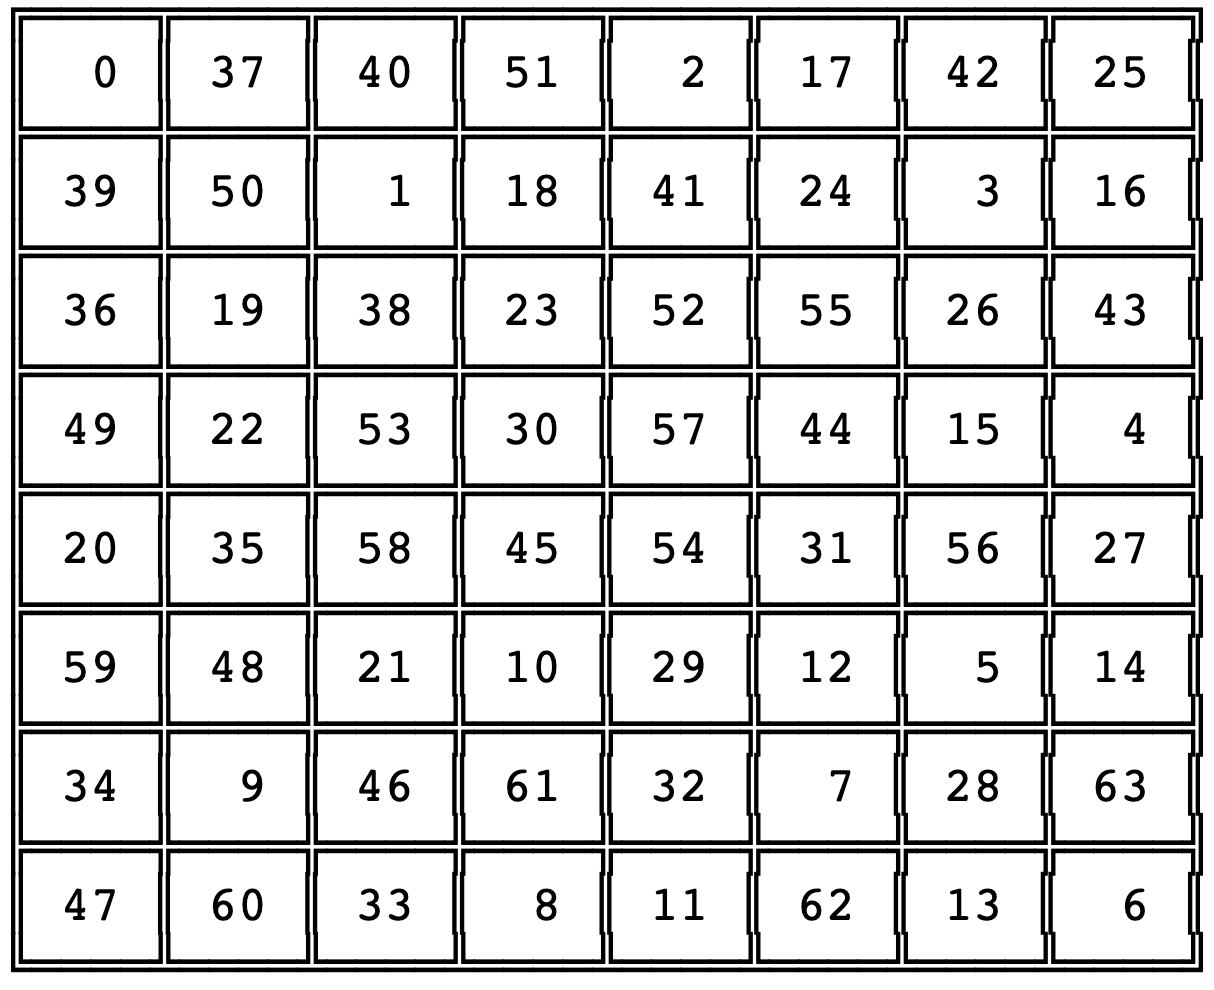
\epsfig{file=Figures/knights-problem.png, scale=0.5}} 
  \caption{A solution of the knight's problem.}
  \label{fig:knights-problem.png}
\end{figure}

Finally, the function \texttt{solve} that is shown in Figure \ref{fig:Knight's Tour with Z3.ipynb-2} on page
\pageref{fig:Knight's Tour with Z3.ipynb-2} can be used to solve the puzzle.
The purpose of the function \texttt{solve} is to construct a \textsc{Csp} encoding the puzzle and to find a
solution of this \textsc{Csp} unsing \texttt{Z3}.
If successful, it returns a dictionary that maps every variable name to the corresponding value of the solution
that has been found.
\begin{enumerate}
\item In line 2 and 3 we create the \texttt{Z3} variables that specify the positions of the knight after its
      $i^{\mathrm{th}}$ move.  $\texttt{Rows}[i]$ specifies the row of the knight after the its
      $i^{\mathrm{th}}$ move, while $\texttt{Cols}[i]$ specifies the column.
\item We compute the set of all constraints in line 4.   
\item We create a solver object in line 5 and add the constraints to this solver in the following line.
\item The function \texttt{check} tries to build a model satisfying the constraints, while the function
      \texttt{model} extracts this model if it exists.
\item Finally, in line 10 and 11 we create a dictionary that maps all of our variables to the corresponding
      values that are found in the model.  Note that $\texttt{row}(i)$ returns the name of the
      \texttt{Z3} variable $\texttt{Rows}[i]$ and similarly $\mathtt{col}(i)$ returns the name of the
      \texttt{Z3} variable $\texttt{Cols}[i]$.
      This dictionary is then returned.
\end{enumerate}
Figure \ref{fig:knights-problem.png} on page \pageref{fig:knights-problem.png} shows a solution that has been
computed by the program discussed above.






\begin{table}[h]
  \centering
  \begin{tabular}{||c|c|c||c|c|c||c|c|c||}
    \hline
    \hline
      & 3 & 9 &   &   &   &   &   & 7 \\
    \hline
      &   &   & 7 &   &   & 4 & 9 & 2 \\
    \hline
      &   &   &   & 6 & 5 &   & 8 & 3 \\
    \hline
    \hline
      &   &   & 6 &   & 3 & 2 & 7 &   \\
    \hline
      &   &   &   & 4 &   & 8 &   &   \\
    \hline
    5 & 6 &   &   &   &   &   &   &   \\
    \hline
    \hline
      &   & 5 & 2 &   & 9 &   &   & 1 \\
    \hline
      & 2 & 1 &   &   &   &   & 4 &   \\
    \hline
    7 &   &   &   &   &   & 5 &   &   \\
    \hline
    \hline
  \end{tabular}
  \caption{A super hard sudoku from the magazine ``Zeit Online''.}
  \label{tab:sudoku}
\end{table}


\exerciseEng
\index{sudoku}
Table \ref{tab:sudoku} on page \pageref{tab:sudoku} shows a \href{https://en.wikipedia.org/wiki/Sudoku}{sudoku}
that I have taken from the
\href{http://sudoku.zeit.de/cgi-bin/sudoku/sudoku_kd_app_2016.pl?action=level&kd_nr=24091123601092&year=2018&month=03&day=23&level=-c+5}{Zeit Online}
magazine.
Solve this sudoku using \texttt{Z3}.  You should start with the following file:
\\[0.2cm]
\hspace*{0.0cm}
\href{https://github.com/karlstroetmann/Logic/blob/master/Python/Chapter-5/Sudoku-Z3.ipynb}{https://github.com/karlstroetmann/Logic/blob/master/Python/Chapter-5/Sudoku-Z3.ipynb}.
    \eox

\subsection{Solving Search Problems with \texttt{Z3}}
In this subsection we show how to solve a search problem using \texttt{Z3}.  The idea is to formulate the
search problem as a symbolic transition system, convert the symbolic transition system into a \textsc{Csp}, and
then solve the \textsc{Csp} using \texttt{Z3}.
We will explain our method by solving the
\href{https://en.wikipedia.org/wiki/Missionaries_and_cannibals_problem}{missionaries and cannibals problem}
that has already been discussed earlier.  

\begin{figure}[!ht]
\centering
\begin{minted}[ frame         = lines, 
                 framesep      = 0.3cm, 
                 firstnumber   = 1,
                 bgcolor       = sepia,
                 numbers       = left,
                 numbersep     = -0.2cm,
                 xleftmargin   = 0.8cm,
                 xrightmargin  = 0.8cm,
               ]{python3}
    M = z3.Int('M')
    C = z3.Int('C')
    B = z3.Int('B')
    
    def start(M, C, B):
        return z3.And(M == 3, C == 3, B == 1)
    
    def goal(M, C, B):
        return z3.And(M == 0, C == 0, B == 0)
    
    def invariant(M, C, B):
        return z3.And(z3.Or(M == 0, M == 3, M == C),
                      0 <= M, M <= 3,
                      0 <= C, C <= 3,
                      0 <= B, B <= 1)
    def transition(M, C, B, Mx, Cx, Bx):
        Formulas  = { Bx == 1 - B }
        Formulas |= { z3.Implies(B == 1, 
                                 z3.And(1 <= M - Mx + C - Cx, 
                                        2 >= M - Mx + C - Cx,
                                        Mx <= M, 
                                        Cx <= C)
                                ),
                      z3.Implies(B == 0, 
                                 z3.And(1 <= Mx - M + Cx - C,
                                        2 >= Mx - M + Cx - C,
                                        Mx >= M, 
                                        Cx >= C)
                                )
                    }
        return z3.And(Formulas)
\end{minted}
\vspace*{-0.3cm}
\caption{Solving The Missionaries-and-Cannibals-Problem with \texttt{Z3}, part \texttt{I}.}
\label{fig:Missionaries-Z3.ipynb-1}
\end{figure}

Figure \ref{fig:Missionaries-Z3.ipynb-1} on page \pageref{fig:Missionaries-Z3.ipynb-1} shows how we can define
the associated symbolic transition system using the constraint solver \texttt{Z3}.
\begin{enumerate}
\item In line 1 -- 3 we define the variables \texttt{M}, \texttt{C}, and \texttt{B}.  These represent the
      number of missionaries, cannibals, and boats on the eastern shore.  We have defined these variables as
      integers, although the set of values really is the set $\{0,1,2,3\}$.  We will later add appropriate
      inequalities to restrict these variables to this set.
\item The definition of \texttt{start} and \texttt{goal} in line 6 and 9 are analogous the corresponding
      definitions in \myfig{Missionaries-STS.ipynb}.  The describe that initially everybody and the boat is on
      the eastern shore, while in the end everybody is on the western shore.

      Note that we have to use the \texttt{Z3} function \texttt{And} to form the conjunction of the conditions.
      The function takes an arbitrary number of arguments.  The constraint solver \texttt{Z3} also provides the
      functions \texttt{Or} and \texttt{Implies}.  The function \texttt{Or} computes the disjunction of its
      arguments, while the function $\texttt{Implies}(A, B)$ represents the formula $A \rightarrow B$.
\item The definition of the invariant in 11 -- 15 has become more complicated because in addition to the
      formula 
      \\[0.2cm]
      \hspace*{1.3cm}
      $M = 0 \vee M = 3 \vee M = C$
      \\[0.2cm]
      we also have to add constraints that restrict the values of $M$ and $C$ to the set $\{0, 1, 2, 3\}$,
      while $B$ has to be an element of the set $\{0,1\}$.
\item The definition of the formula describing the transitions of the symbolic transition system is 
      analogous to the corresponding definition in \myfig{Missionaries-STS.ipynb}.
\end{enumerate}

\begin{figure}[!ht]
\centering
\begin{minted}[ frame         = lines, 
                 framesep      = 0.3cm, 
                 firstnumber   = 1,
                 bgcolor       = sepia,
                 numbers       = left,
                 numbersep     = -0.2cm,
                 xleftmargin   = 0.8cm,
                 xrightmargin  = 0.8cm,
               ]{python3}
    def missionaries_CSP(n):
        S = z3.Solver()
        Ms = [z3.Int(f'M{i}') for i in range(n+1)]
        Is = [z3.Int(f'C{i}') for i in range(n+1)]
        Bs = [z3.Int(f'B{i}') for i in range(n+1)]
        Constraints  = { start(Ms[0], Is[0], Bs[0]) }  # start state
        Constraints |= { goal( Ms[n], Is[n], Bs[n]) }  # goal state
        for i in range(n):
            Constraints.add(invariant(Ms[i], Is[i], Bs[i]))
            Constraints.add(transition(Ms[i  ], Is[i  ], Bs[i  ], 
                                       Ms[i+1], Is[i+1], Bs[i+1]))
        S.add(Constraints)
        result = str(S.check())
        if result == 'sat':
            Model = S.model()
            Solution = (   { f'M{i}': Model[Ms[i]] for i in range(n+1) }
                         | { f'C{i}': Model[Is[i]] for i in range(n+1) }
                         | { f'B{i}': Model[Bs[i]] for i in range(n+1) }
                       )
            return { key: Solution[key].as_long() for key in Solution }            
        else:
            return None
    
    def find_solution():
        n = 1
        while True:
            print(n)
            Solution = missionaries_CSP(n)
            if Solution != None:
                return n, Solution
            n += 2    
\end{minted}
\vspace*{-0.3cm}
\caption{Solving The Missionaries-and-Cannibals-Problem with \texttt{Z3}, part \texttt{II}.}
\label{fig:Missionaries-Z3.ipynb-2}
\end{figure}

Figure \ref{fig:Missionaries-Z3.ipynb-2} on page \pageref{fig:Missionaries-Z3.ipynb-2} show the implementation
of the function \texttt{missionaries\_CSP} that takes a natural number $n$ as its input and then creates a
\textsc{Csp} that is solvable if and only if the symbolic transition system shown in
\myfig{Missionaries-Z3.ipynb-1} has a solution involving $n$ transitions.
\begin{enumerate}
\item Line 2 creates the solver object \texttt{S}.
\item Line 3--5 create the associated variables.
\item Line 6 creates the constraint corresponding to the initial state of the symbolic transition system.
\item Line 7 creates the constraint corresponding to the goal state.
\item The \texttt{for}-loop in line 8 ensures two things:
  \begin{enumerate}[(a)]
  \item Every intermediate state has to satisfy the invariant.
  \item Every transition from a state to the successor state has to satisfy the transition formula.
  \end{enumerate}
\item Line 12 feeds the constraints to the solver.
\item Line 13 checks whether the resulting \textsc{Csp} is solvable.
\item If it is solvable, we return a dictionary that associates every variable $\texttt{M}_i$,  $\texttt{C}_i$,
      $\texttt{B}_i$ with the corresponding value of the solution.
\item The function \texttt{find\_solution} searches for a value of $n \in \mathbb{N}$ such that the problem is
      solvable in $n$ steps.
\end{enumerate}
At this point you might well ask whether there is any benefit if we solve this problem with \texttt{Z3}.  The
answer is that it is about efficiency.  While our simple backtracking solver took 1.5 seconds to solve this
problem, \texttt{Z3} takes only 0.113 seconds to compute the solution.  In the following exercise you will
solve a more complicated search problem which would take much too long to solve if we would only use backtracking.

\exerciseEng
The following puzzle is part of a recruitment test in Japan.

\begin{minipage}{0.95\linewidth}
{\sl
  A policeman, a convict, a father and his two sons Anton and Bruno, and a mother with her two daughters Cindy and Doris have to cross a river. On the boat there is only room for two passengers.
During the crossing, the following conditions have to be observed:
\begin{enumerate}[(a)]
\item The father is not allowed to be on a shore with one of the daughters if the mother is on the other shore.
\item The mother is not allowed to be on a shore with one of the sons if the father is on the other shore.
\item If the convict is not alone, then the policeman must watch him.
\item However the convict can be alone on a shore, as his shackles prevent him from running away.
\item Only the father, the mother, and the policeman are able to steer the boat.
\end{enumerate}}
\end{minipage}

\noindent
Your task is to solve this puzzle by coding it as a symbolic transition system.  You should then solve the
transition system using the constraint solver \texttt{Z3}.
Start with the following file:
\\[0.2cm]
\hspace*{0.0cm}
\href{https://github.com/karlstroetmann/Logic/blob/master/Python/Chapter-5/Japanese-Z3.ipynb}{https://github.com/karlstroetmann/Logic/blob/master/Python/Chapter-5/Japanese-Z3.ipynb}.
\eox
\pagebreak

\exerciseEng
The following puzzle offers a new twist to the river crossing puzzles encountered before, because we have to
take the time used for a crossing into account.

\begin{minipage}{0.95\linewidth}
  {\sl
    In the darkness of the night, a group of four individuals encounters a river. A slender bridge stretches
    before them, capable of accommodating just two people simultaneously. Equipped with a single torch, they
    must rely on its flickering light to navigate the bridge. Each person possesses a distinct crossing time:
    Ariela takes 1 minute, Brian takes 2 minutes, Charly takes 5 minutes, and Dumpy takes 8 minutes. It is
    crucial to note that when two people cross together, they must synchronize their steps with the slower
    individual's pace. Given the torch's limited lifespan of 15 minutes, the pressing question arises: can all
    four individuals successfully traverse the bridge? 
  }
\end{minipage}

\noindent
Your task is to solve this puzzle by coding it as a symbolic transition system.  You should then solve the
transition system using the constraint solver \texttt{Z3}.
Start with the following file:
\\[0.2cm]
\hspace*{0.0cm}
\href{https://github.com/karlstroetmann/Logic/blob/master/Python/Chapter-5/Bridge-Torch.ipynb}{https://github.com/karlstroetmann/Logic/blob/master/Python/Chapter-5/Bridge-Torch.ipynb}.
\eox

\section{Normalizing First-Order Formulas}
In the next section, we will define a calculus $\vdash$ for first-order logic. Just as in the case of
propositional logic, this will be much easier if we restrict ourselves to formulas that are in a \blue{normal form}. 
This normal form consists of so-called \blue{first-order clauses}.\index{first-order clause}
These are defined similarly as in propositional logic: A \blue{first-order literal}\index{first-order literal}
is an atomic formula or the negation of an atomic formula. A \blue{first-order clause}\index{predicate logic clause} 
is a disjunction of first-order literals. We show in this section that every set of formulas $M$ can be
transformed into a set of first-order clauses $K$ such that 
$M$ is satisfiable if and only if $K$ is satisfiable. Therefore, the restriction to first-order clauses is
not a real restriction. First, we specify some equivalences that can be used to manipulate quantifiers.

\begin{Satz}
  The following equivalences are valid in first-order logic:
  \begin{enumerate}
  \item $\models \neg\big(\forall x\colon f\big) \leftrightarrow \big(\exists x\colon \neg f\big)$
  \item $\models \neg\big(\exists x\colon f\big) \leftrightarrow \big(\forall x\colon \neg f\big)$
  \item $\models \forall x\colon f \wedge \forall x\colon g \leftrightarrow \forall x\colon (f \wedge g)$
  \item $\models \exists x\colon f \vee \exists x\colon g \leftrightarrow \exists x\colon (f \vee g)$
  \item $\models \forall x\colon \forall y\colon f \leftrightarrow \forall y\colon  \forall x\colon f$
  \item $\models \exists x\colon \exists y\colon f \leftrightarrow \exists y\colon  \exists x\colon f$
  \item If $x$ is a variable such that $x \not\in \FV(f)$, then \\[0.2cm]
        \hspace*{1.3cm} $\models  (\forall x\colon f) \leftrightarrow f$ \quad and \quad
                        $\models  (\exists x\colon f) \leftrightarrow f$.
  \item If $x$ is a variable such that $x \not\in \FV(g)$, then:
    \begin{enumerate}
    \item $\models (\forall x\colon f) \vee g \leftrightarrow \forall x\colon (f \vee g)$ \quad and \quad $\models g \vee (\forall x\colon f) \leftrightarrow \forall x\colon (g \vee f)$,
    \item $\models (\exists x\colon f) \wedge g \leftrightarrow \exists x\colon (f \wedge g)$ \quad and \quad $\models g \wedge (\exists x\colon f) \leftrightarrow \exists x\colon (g \wedge f)$.
    \end{enumerate}
  \end{enumerate}
\end{Satz}

In order to apply the equivalences of the last group, it may be necessary to rename bound variables. If $f$ is a first-order logic formula and $x$ and $y$ are two variables, where $y$ does not appear in $f$, then \blue{$f[x/y]$} denotes the formula that results from $f$ by replacing every occurrence of the variable $x$ in $f$ with $y$. For example, \\[0.2cm]
\hspace*{1.3cm} $\bigl(\forall u : \exists v : p(u,v)\bigr)[u/z] = \forall z : \exists v : p(z,v)$
\\[0.2cm]
With this we can specify one last equivalence: If $f$ is a first-order logic formula, $x \in BV(f)$ and $y$ is a variable that does not appear in $f$, then \\[0.2cm]
\hspace*{1.3cm} $\models f \leftrightarrow f[x/y]$.
\vspace{0.3cm}

Using the equivalences given above together with the equivalences from propositional logic we are able
to transform every first order formula into a form where the quantifieres are all at the beginning of the
formula, i.e.~the formula has the form
\\[0.2cm]
\hspace*{1.3cm}
$Q_1 x_1: Q_2 x_2: \cdots Q_n x_n: G$ \quad where $Q_i \in \{ \forall, \exists \}$ f.a.~$i=1,\cdots,n$
\\[0.2cm]
and $G$ does not contain quantifieres.  A formula of this form is in 
\blue{prenex normal form}.\index{prenex normal form}  We demonstrate this procedure with an example and show
that the formula
\\[0.2cm]
\hspace*{1.3cm}
$\bigl(\forall x\colon p(x)\bigr) \rightarrow \bigl(\exists x\colon p(x)\bigr)$ 
\\[0.2cm]
is universally valid: 
$$ 
\begin{array}{ll}
                 & \bigl(\forall x\colon p(x)\bigr) \rightarrow \bigl(\exists x\colon p(x)\bigr)  \\
 \Leftrightarrow & \neg \bigl(\forall x\colon p(x)\bigr) \vee \bigl(\exists x\colon p(x)\bigr)    \\
 \Leftrightarrow & \bigl(\exists x\colon \neg p(x)\bigr) \vee \bigl(\exists x\colon p(x)\bigr)    \\
 \Leftrightarrow & \exists x\colon \bigl(\neg p(x) \vee p(x)\bigr) \\
 \Leftrightarrow & \exists x\colon \verum                                                  \\
 \Leftrightarrow & \verum                                                  \\
\end{array}
$$
\\[0.2cm]
In this case, we were lucky that we managed to recognise the formula as a tautology.
In general, however, the above transformations are not sufficient to recognise
whether a first order formula is universally valid. 
To be able to simplify formulas even more, 
we introduce another concept of equivalence.  We want to motivate this term with an example.
We look at the following formulas
\\[0.2cm]
\hspace*{1.3cm} $f_1 = \forall x \colon \exists y \colon p(x,y)$ \quad und \quad $f_2 = \forall x \colon
p\bigl(x,s(x)\bigr)$.
\\[0.2cm]
The two formulae $f_1$ and $f_2$ are not equivalent, because they do not even originate from the same signature.
In the formula $f_2$, the function character $s$
is used, which does not appear at all in the formula $f_1$. 
Even if the two formulae $f_1$ and $f_2$ are not equivalent, the following relationship exists between them: If
$\textsl{S}_1$ is a 
$\Sigma$-structure in which the formula $f_1$ holds, i.e.
\\[0.2cm]
\hspace*{1.3cm}
$\mathcal{S}_1 \models f_1$,
\\[0.2cm]
then we can extend the $\Sigma$-structure to a $\Sigma'$-structure  $\textsl{S}_2$ such that
$f_2$ is valid in $\mathcal{S}_2$:
\\[0.2cm]
\hspace*{1.3cm}
$\mathcal{S}_2 \models f_2$.
\\[0.2cm]
To do this, the interpretation of the function character $s$ has to be chosen such that
$p\bigl(x,s(x)\bigr)$ actually holds for each $x$.  This is possible because the formula $f_1$ states 
that for every $x$ there is a value $y$ such that $p(x,y)$ holds.  The function $s$ therefore has to 
return this $y$ for every $x$. 

\begin{Definition}[{\color{blue}Skolemisation}]\index{Skolemisation} \hspace*{\fill} \linebreak
  Assume $\Sigma = \langle \mathcal{V}, \mathcal{F}, \mathcal{P}, \textsl{arity} \rangle$
  is a signature.  Furthermore, let $f$ be a closed $\Sigma$ formula of the form \\[0.2cm]
  \hspace*{1.3cm} 
  $f = \forall x_1, \cdots, x_n \colon \exists y \colon g$. \\[0.2cm]
  Then we choose an \underline{\blue{new}} $n$-digit function character $s$, i.e.~we take a character $s$ that
  is not used in the  signature $\Sigma$ and extend the signature $\Sigma$ to the signature \\[0.2cm]
  \hspace*{1.3cm} 
  $\Sigma' := \Bigl\langle \mathcal{V}, \mathcal{F} \cup \{s\}, \mathcal{P}, \textsl{arity} \cup \bigl\{\pair(s,n)\bigr\} \bigr\rangle$, \\[0.2cm]
  where $s$ is declared as a new $n$-digit function character.  Then we define the $\Sigma'$ formula
  $f'$ as follows: \\[0.2cm]
  \hspace*{1.3cm} 
  $f' := \mathtt{Skolem}(f) := 
  \forall x_1 \colon \cdots \forall x_n \colon g\bigl[y \mapsto s(x_1,\cdots,x_n)\bigr]$
  \\[0.2cm]
  Here, the expression $g\bigl[y \mapsto s(x_1,\cdots,x_n)\bigr]$ denotes the formula that we obtain from $g$
  by replacing each occurrence of the variable $y$ in the formula $g$ by the term
  $s(x_1,\cdots,x_n)$.  We say that the formula $f'$ results from the formula $f$  through one \blue{Skolemisation step}. 
  \eox
\end{Definition}

\exampleEng
It $f$ the following formula from group theory:
\\[0.2cm]
\hspace*{1.3cm}
$f := \forall x: \exists y: y * x = 1$. 
\\[0.2cm]
Then the following holds:
\\[0.2cm]
\hspace*{1.3cm}
$\mathtt{Skolem}(f) = \forall x : s(x) * x = 1$.  \eox

\noindent
In what sense are a formula $f$ and a formula $f'$, which are derived from $f$ by a 
Skolem\-isation step equivalent?  We answer this question with the following definition. 

\begin{Definition}[Satisfiability Equivalence] \hspace*{\fill} \linebreak
   Two closed formulas $f$ and $g$ are called 
   \blue{satisfiability-equivalent}\index{satisfiability-equivalent}
   if $f$ and $g$ are either both satisfiable or both unsatisfiable.
   If $f$ and $g$ are satisfiability-equivalent, we write \\[0.2cm]
   \hspace*{1.3cm} $f \approx_e g$.
\eox
\end{Definition}

\noindent
\textbf{Observation:}
If the formula $f'$ is derived from the formula $f$ by a skolemisation step, i.e.~if we have that $f' = \mathtt{Skolem} (f)$
then $f$ and $f'$ are satisfiability-equivalent, because we can transform any structure
$\mathcal{S}$ such that $\mathcal{S} \models f$ into a structure $\mathcal{S}'$ such that
$\mathcal{S}' \models f'$.  Therefore we have
\\[0.2cm]
\hspace*{1.3cm}
$f \approx_e \mathtt{Skolem}(f)$. \eox


We can now specify a simple procedure to eliminate existential quantifiers from a formula.  This procedure
consists of two steps:
\begin{itemize}
\item First, we put the formula into prenex normal form. 
\item Then we can eliminate the existential quantifiers one by one using Skolemisation steps.
\end{itemize}
The resulting formula is then satisfiability-equivalent to the original formula.  This
process of eliminating existential quantifiers through the introduction of new function
function characters is called \blue{Skolemisation}.  If we have a formula $F$
into prenex normal form and then skolemised it, the result has the form\\[0.2cm]
\hspace*{1.3cm} $\forall x_1, \cdots, x_n: g$ \\[0.2cm]
and there are no more quantifiers in the formula $g$.  The formula $g$ is also known as the
\blue{matrix}\index{matrix} of the above formula.  We can now transform $g$ with the help of
of the propositional equivalences known from the last chapter into conjunctive normal form.  We then have a
formula of the form \\[0.2cm]
\hspace*{1.3cm} $\forall x_1, \cdots, x_n: (k_1 \wedge \cdots \wedge k_m)$. \\[0.2cm]
The $k_i$ are disjunctions of first-order \blue{literals}.  Next, we apply  the equivalence 
\\[0.2cm]
\hspace*{1.3cm}
$\forall x\colon (f_1\wedge f_2) \leftrightarrow (\forall x\colon f_1) \wedge (\forall x\colon f_2)$.
\\[0.2cm]
In this way we can distribute the universal-quantifiers to the individual $k_i$.
The resulting formula has the form \\[0.2cm]
\hspace*{1.3cm} 
$\big(\forall x_1, \cdots, x_n: k_1\big) \wedge \cdots \wedge \big(\forall x_1, \cdots, x_n: k_m\big)$.
\\[0.2cm]
If a formula $F$ has this form, we say that $F$ is in \blue{first-order clause normal form}
\index{first-order clause normal form} and a formula of the form \\[0.2cm]
\hspace*{1.3cm} $\forall x_1, \cdots, x_n: k$, \\[0.2cm]
where $k$ is a disjunction of first-order literals,
is called a \blue{first-order clause}.  \index{predicate logical clause} If $M$ is
is a set of formulas whose satisfiability we want to analyse, 
we can always transform $M$ into a satisfiability-equivalent set of first-order clauses.
Since then only universal-quantifiers occur, we can simplify the notation
by agreeing that all formulae are implicitly universally quantified, i.e. we omit
the universal quantifiers.


\noindent
The Jupyter notebook
\\[0.2cm]
\hspace*{0.8cm}
\href{https://github.com/karlstroetmann/Logic/blob/master/Python/Chapter-5/FOL-CNF.ipynb}{https://github.com/karlstroetmann/Logic/blob/master/Python/Chapter-5/FOL-CNF.ipynb}.
\\[0.2cm]
contains a \textsl{Python} programme that we can use to transform predicate logic formulae into a 
satisfiability-equivalent set of predicate logic clauses.

Our goal is to develop a method that can be used to verify that a first-order formula
$f$ is universally valid, i.e.~we want to be able to prove that \\[0.2cm]
\hspace*{1.3cm}
$\models f$
\\[0.2cm]
holds.  We know that \\[0.2cm]
\hspace*{1.3cm}
$\models f$ \quad if and only if \quad $\{\neg f\} \models \falsum$, \\[0.2cm]
because the formula $f$ is universally valid iff there is no $\Sigma$-structure $\mathcal{S}$ such that
\\[0.2cm]
\hspace*{1.3cm}
$\mathcal{S} \models \neg f$,
\\[0.2cm]
i.e.~$f$ is universally valid iff $\neg f$ is unsatisfiable. 
Therefore, in oder to prove that $f$ is universally valid, we transform the formula $\neg f$  into 
first-order normal form.  By doing this we obtain clauses $k_1, \cdots, k_n$ such that \\[0.2cm]
\hspace*{1.3cm} $\neg f \approx_e k_1 \wedge \cdots \wedge k_n$ \\[0.2cm]
holds.  Next,  we try to
derive a contradiction from the clauses $k_1,\cdots,k_n$: \\[0.2cm]
\hspace*{1.3cm} $\{k_1, \cdots, k_n\} \vdash \falsum$ \\[0.2cm]
If this succeeds, then we know that the set $\{k_1, \cdots, k_n\}$ is unsatisfiable.
This means that $\neg f$ is also unsatisfiable and hence $f$ must be universally valid.
In order to derive a contradiction from the clauses $k_1,\cdots,k_n$
we need a calculus $\vdash$ that works with first-order clauses. 
We will present this calculus in section \ref{sec:fol-calculus}.

To explain the procedure in more detail, we will demonstrate it using an example. 
We want to investigate whether 
\\[0.2cm]
\hspace*{1.3cm} 
$\models \big(\exists x\colon \forall y\colon  p(x,y)\big) \rightarrow \big(\forall y\colon \exists x\colon p(x,y)\big)$ \\[0.2cm]
holds. We know that this is equivalent to  \\[0.2cm]
\hspace*{1.3cm} 
$\Big\{ \neg \Big(\big(\exists x\colon \forall y\colon  p(x,y)\big) \rightarrow  \big(\forall y\colon \exists
x\colon p(x,y)\big)\Big)\Big\} \models \falsum$.
\\[0.2cm]
Therefore we transform the negated formula in prenex normal form.
$$
\begin{array}{ll}
                  & \neg \Big(\big(\exists x\colon \forall y\colon  p(x,y)\big) \rightarrow \big(\forall y\colon \exists x\colon p(x,y)\big)\Big) \\
  \leftrightarrow & \neg \Big(\neg \big(\exists x\colon \forall y\colon  p(x,y)\big) \vee \big(\forall y\colon \exists x\colon p(x,y)\big)\Big) \\
  \leftrightarrow &                \big(\exists x\colon \forall y\colon  p(x,y)\big) \wedge \neg \big(\forall y\colon \exists x\colon p(x,y)\big) \\
  \leftrightarrow &\big(\exists x\colon \forall y\colon  p(x,y)\big) \wedge  \big(\exists y\colon  \neg \exists x\colon p(x,y)\big) \\
  \leftrightarrow &\big(\exists x\colon \forall y\colon  p(x,y)\big) \wedge  \big(\exists y\colon  \forall x\colon \neg p(x,y)\big) \\
\end{array}
$$
In order to proceed we have to rename the variables in the second part of the formula.
We replace $x$ with $u$ and $y$ with $v$ and are left with the following:
$$
\begin{array}{ll}
                  &\big(\exists x\colon \forall y\colon  p(x,y)\big) \wedge  \big(\exists y\colon  \forall x\colon \neg p(x,y)\big) \\
  \leftrightarrow &\big(\exists x\colon \forall y\colon  p(x,y)\big) \wedge  \big(\exists v\colon  \forall u\colon \neg p(u,v)\big) \\
  \leftrightarrow &\exists v\colon  \Big( \big(\exists x\colon \forall y\colon  p(x,y)\big) \wedge  \big(\forall u\colon \neg p(u,v)\big) \Big)\\
  \leftrightarrow &\exists v\colon  \exists x\colon  \Big( \big(\forall y\colon  p(x,y)\big) \wedge \big(\forall u\colon \neg p(u,v)\big) \Big)\\
  \leftrightarrow &\exists v\colon  \exists x\colon \forall y\colon \Big( p(x,y) \wedge \big(\forall u\colon \neg p(u,v)\big) \Big)\\
  \leftrightarrow &\exists v\colon  \exists x\colon \forall y\colon \forall u\colon \Big( p(x,y) \wedge \neg p(u,v) \Big)\\
\end{array}
$$
Now we have to skolemize in order to get rid of the existential quantifiers.
In order to do this, we introduce two new function symbols $s_1$ and $s_2$. 
We have both  $\mathtt{arity}(s_1) = 0$ and $\mathtt{arity}(s_2) = 0$, because the existential quantifiers are
not preceded by universal quantifiers.
$$
\begin{array}{ll}
           & \exists v\colon  \exists x\colon \forall y\colon \forall u\colon \Big( p(x,y) \wedge \neg p(u,v) \Big)\\
 \approx_e & \exists x\colon \forall y\colon \forall u\colon \Big( p(x,y) \wedge \neg p(u,s_1) \Big)\\
 \approx_e & \forall y\colon \forall u\colon \Big( p(s_2,y) \wedge \neg p(u,s_1) \Big)\\
\end{array}
$$
At this point we are left with  universal quantifiers.  These can be omitted,
as we have already agreed that all free variables are implicitly universally quantified.
We proceed to present the first order CNF of our formula in set notation:
\\[0.2cm] 
\hspace*{1.3cm}
$M := \Big\{ \big\{ p(s_2,y) \big\}, \big\{\neg p(u,s_1)\big\}\Big\}$.
\\[0.2cm]
Next, we show that the set $M$ is contradictory.
To do this, we first consider the clause $\big\{ p(s_2,y) \big\}$ and insert 
the constant $s_1$ in this clause for $y$.  This gives us the clause \\[0.2cm]
\hspace*{1.3cm} $\big\{ p(s_2,s_1) \big\}$. \hspace*{\fill}(1)\\[0.2cm]
We justify the replacement of $y$ by $s_1$ by the fact that the above clause is implicitly
universally quantified and if something is true for all $y$, then it is certainly also true for $y = s_1$.

Next, we take the clause $\big\{\neg p(u,s_1)\big\}$ and
insert the constant $s_2$ for the variable $u$.  We obtain the 
clause \\[0.2cm]
\hspace*{1.3cm} $\big\{\neg p(s_2,s_1)\big\}$ \hspace*{\fill} (2) \\[0.2cm]
Now we apply the cut rule to the clauses (1) and (2) and have \\[0.2cm]
\hspace*{1.3cm} 
$\big\{ p(s_2,s_1) \big\}$, \quad$\big\{\neg p(s_2,s_1)\big\}$ \quad $\vdash \quad \{\}$.
\\[0.2cm]
We have thus derived a contradiction and shown that the set $M$ is unsatisfiable.  Therefore, we also know that
\\[0.2cm]
\hspace*{1.3cm} 
$\Big\{ \neg \Big(\big(\exists x\colon \forall y\colon  p(x,y)\big) \rightarrow  \big(\forall y\colon \exists x\colon p(x,y)\big)\Big)\Big\}$
\\[0.2cm]
is unsatisfiable and hence we have shown \\[0.2cm]
\hspace*{1.3cm} 
$\models \big(\exists x\colon \forall y\colon  p(x,y)\big) \rightarrow  \big(\forall y\colon \exists x\colon p(x,y)\big)$.

\section{Unification}
This section introduces the notion of a \blue{most general unifier} of two terms.
First, we define the notion of a $\Sigma$-substitution.

\begin{Definition}[$\Sigma$-Substitution]
  Assume that a signature $\Sigma = \langle \mathcal{V}, \mathcal{F}, \mathcal{P}, \textsl{arity} \rangle$ is given.
  A \blue{$\Sigma$-substitution} $\sigma$ is a map of the form
  \\[0.2cm]
  \hspace*{1.3cm}
  $\sigma: \mathcal{V} \rightarrow \mathcal{T}_\Sigma$ 
  \\[0.2cm]
  such that the set $\textsl{dom}(\sigma) := \bigl\{ x \in \mathcal{V} \mid \sigma(x) \not= x \bigr\}$ is finite.
  If we have $\textsl{dom}(\sigma) = \{ x_1, \cdots, x_n \}$ and $t_i = \sigma(x_i)$ for all $i = 1, \cdots, n$,
  then we use the following notation:
  \\[0.2cm]
  \hspace*{1.3cm}
  $\sigma = \{ x_1 \mapsto t_1, \cdots, x_n \mapsto t_n \}$.
  \\[0.2cm]
  The set of all $\Sigma$-Substitutions is denoted as $\mathtt{Subst}(\Sigma)$.
  \eox
\end{Definition}

A substitution $\sigma = \{ x_1 \mapsto t_1, \cdots, x_n \mapsto t_n \}$ can be \blue{applied} to a term $t$
by replacing the variables $x_i$ with the terms $t_i$.  We will use the postfix notation \blue{$t\sigma$} to denote the
\blue{application} of the substitution $\sigma$ to the term $t$.  Formally, the notation $t \sigma$ is defined
by induction on $t$:
\begin{enumerate}
\item $x \sigma := \sigma(x)$ \quad for all $x \in \mathcal{V}$.
\item $c \sigma = c$ \quad for every constant $c \in \mathcal{F}$.
\item $f(t_1, \cdots, t_n) \sigma := f\bigl(t_1\sigma, \cdots, t_n\sigma\bigr)$.
\end{enumerate}



Next, we define the composition of two $\Sigma$-substitutions.

\begin{Definition}[Composition of Substitutions] \index{Composition von Substitutions}
    Assume that \\[0.2cm]
    \hspace*{1.3cm}
    $\sigma = \{ x_1 \mapsto s_1, \cdots, x_m \mapsto s_m \}$
    \quad and \quad
    $\tau = \{ y_1 \mapsto t_1, \cdots, y_n \mapsto t_n \}$
    \\[0.2cm]
    are two substitutions such that $\textsl{dom}(\sigma) \cap \textsl{dom}(\tau) = \{\}$.
    We define the  \blue{composition $\sigma\tau$} \index{composition $\sigma\tau$} of $\sigma$ and $\tau$  as
    \\[0.2cm]
    \hspace*{1.3cm}
    $\sigma\tau := \{ x_1 \mapsto s_1\tau, \cdots, x_m \mapsto s_m\tau,\; y_1 \mapsto t_1, \cdots, y_n \mapsto t_n \}$
    \eox
\end{Definition}

\exampleEng
If we define
\\[0.2cm]
\hspace*{1.3cm}
$\sigma := \{ x_1 \mapsto c,\; x_2 \mapsto f(x_3) \}$ \quad and \quad
$\tau := \{ x_3 \mapsto h(c,c),\; x_4 \mapsto d \}$,
\\[0.2cm]
then we have
\\[0.2cm]
\hspace*{1.3cm}
$\sigma\tau = \{ x_1 \mapsto c,\; x_2 \mapsto f(h(c,c)),\; x_3 \mapsto h(c,c),\;x_4 \mapsto d \}$.
\eox
\vspace{0.3cm}

\begin{Proposition} \label{satz:composition}
    If $t$ is a term and $\sigma$ and $\tau$ are substitutions such that  
    $\textsl{dom}(\sigma) \cap \textsl{dom}(\tau) = \{\}$ holds, then we have
    \\[0.2cm]
    \hspace*{1.3cm} $(t \sigma)\tau = t (\sigma\tau)$.
    \eox
\end{Proposition}
This proposition may be proven by induction on $t$.

\begin{Definition}[Syntactical Equation] \index{syntactical equation}
  A  \blue{syntactical equation} is a pair $\langle s, t \rangle$ of terms.
  It is written as $s \doteq t$. \index{$s \doteq t$}
  A \blue{system of syntactical equations} \index{system of syntactical equations} is a set of syntactical
  equations.
  \eox
\end{Definition}


\begin{Definition}[Unifier]
  A substitution $\sigma$ \blue{solves} a syntactical equation $s \doteq t$ iff we have $s\sigma = t\sigma$.
  If $E$ is a system of syntactical equations and $\sigma$ is a substitution that solves
  every syntactical equations in $E$, then $\sigma$ is a  \blue{unifier} \index{unifier} of $E$.
  \eox
\end{Definition}

\noindent
If $E = \{ s_1 \doteq t_1, \cdots, s_n \doteq t_n \}$ is a system of syntactical equations and $\sigma$ is a
substitution, then we define
\\[0.2cm]
\hspace*{1.3cm}  $E\sigma := \{ s_1\sigma \doteq t_1\sigma, \cdots, s_n\sigma \doteq t_n\sigma \}$.
\vspace{0.3cm}

\exampleEng
Let us consider the syntactical equation
\\[0.2cm]
\hspace*{1.3cm}
$p(x_1, f(x_4)) \doteq p( x_2, x_3)$
\\[0.2cm]
and define the substitution
\\[0.2cm]
\hspace*{1.3cm}
$\sigma := \{ x_1 \mapsto x_2,\; x_3 \mapsto f(x_4) \}$.
\\[0.2cm]
Then $\sigma$ solves the given syntactical equation because we have
\\[0.2cm]
\hspace*{1.3cm}
$p(x_1, f(x_4))\sigma = p(x_2, f(x_4))$ \quad und \quad \\[0.2cm]
\hspace*{1.3cm}
$p(x_2, x_3)\sigma \;\quad = p(x_2, f(x_4))$.  \eox

Next we develop an algorithm for solving a system of syntactical equations.
The algorithm we present was published by Martelli and Montanari
\cite{martelli:1982}.\index{algorithm of Martelli and Montanari}  
To begin, we first consider the cases where a syntactical equation $s \doteq t$ is \blue{unsolvable}.
There are two cases: A syntactical equation of the form
\\[0.2cm]
\hspace*{1.3cm}
$f(s_1,\cdots,s_m) \doteq g(t_1,\cdots, t_n)$ \\[0.2cm]
is certainly unsolvable if  $f$ and $g$ are different function symbols. The reason is that for any substitution
$\sigma$ we have that \\[0.2cm]
\hspace*{1.0cm} $f(s_1,\cdots,s_m)\sigma = f(s_1\sigma,\cdots,s_m\sigma)$ \quad und \quad
                $g(t_1,\cdots, t_n)\sigma = g(t_1\sigma,\cdots,t_n\sigma)$. \\[0.2cm]
If $f \not = g$, then the terms  $f(s_1,\cdots,s_m)\sigma$ and $g(t_1,\cdots, t_n)\sigma$ start with different
function symbols and hence they can't be identical.

The other case where a syntactical equation is unsolvable, is a syntactical equation of the following form:
\\[0.2cm]
\hspace*{1.3cm}
$x \doteq f(t_1,\cdots,t_n)$  \quad where $x \in \texttt{var}\big(f(t_1,\cdots,t_n)\big)$.
\\[0.2cm]
This syntactical equation is unsolvable because the term $f(t_1,\cdots,t_n)\sigma$ will always contain at least one more
occurrence of the function symbol $f$ than the term $x\sigma$.

Now we are able to present an algorithm for solving a system of syntactical equations, provided the system is
solvable.  The algorithm will also discover if a system of syntactical equations is unsolvable.
The algorithm works on pairs of the form
$\langle F, \tau \rangle$ where $F$ is a system of syntactical equations and $\tau$ is a substitution.
The algorithm starts with the pair 
$\langle E, \{\} \rangle$.  Here $E$ is the system of syntactical equations that is to be solved and $\{\}$
represents the empty substitution.  The system works by simplifying the pairs $\langle F, \tau \rangle$ using
certain reduction rules that are presented below.  These reduction rules are applied until we either discover
that the system of syntactical equations is unsolvable or else we reduce the pairs until we finally arrive at a
pair of the form $\langle \{\}, \mu \rangle$.  In this case  $\mu$ is a unifier of the system of
syntactical equations $E$.  The reduction rules are as follows:
\begin{enumerate}
\item If  $y\in\mathcal{V}$ is a variable that does  \underline{\color{red}not} occur in the term $t$, then
      we can perform the following reduction: 
      \[ \Big\langle E \cup \big\{ y \doteq t \big\}, \sigma \Big\rangle \quad\leadsto\quad 
         \Big\langle E\{y \mapsto t\}, \sigma\{ y \mapsto t \} \Big\rangle \qquad\mbox{if $y \in \mathcal{V}$
           and $y \not\in \mathtt{var}(t)$} 
      \]
      This reduction rule can be understood as follows: If the system of syntactical equations that is to be
      solved contains a syntactical equation of the form $y \doteq t$, where the variable $y$ does not occur in
      the term $t$, then the syntactical equation $y \doteq t$ can be removed if we apply the substitution
      $\{ y \mapsto t \}$ to both components of the pair
      \\[0.2cm]
      \hspace*{1.3cm}
      $\Big\langle E \cup \big\{ y \doteq t \big\}, \sigma \Big\rangle$.
\item If the variable $y$ occurs in the term $t$, i.e.~if  $y \in \textsl{Var}(t)$
      and, furthermore, $t \not= y$, then the system of syntactical equations
      $E \cup \big\{ y \doteq t \big\}$ has no solution.  We write this as
      \\[0.2cm]
      \hspace*{1.3cm}
      $\Big\langle E \cup \big\{ y \doteq t \big\}, \sigma \Big\rangle\;\leadsto\; \Omega$ \quad
      if $y \in \texttt{var}(t)$ and $y \not=t$.
\item If $y\in\mathcal{V}$ and  $t \not\in \mathcal{V}$, then we have:
      \[ \Big\langle E \cup \big\{ t \doteq y \big\}, \sigma \Big\rangle \quad\leadsto\quad 
         \Big\langle E \cup \big\{ y \doteq t \big\}, \sigma \Big\rangle \qquad\mbox{if $y \in \mathcal{V}$ and
           $t \not\in \mathcal{V}$.}
      \]   
      After we apply this rule, we can apply either the first or the second reduction rule thereafter.
\item Trivial syntactical equations can be deleted:
      \[ \Big\langle E \cup \big\{ x \doteq x \big\}, \sigma \Big\rangle \quad\leadsto\quad
         \Big\langle E, \sigma \Big\rangle \qquad\mbox{if $x \in \mathcal{V}$.}
      \]   
\item If $f$ is an  $n$-ary function symbol we have 
      \[ \Big\langle E \cup \big\{ f(s_1,\cdots,s_n) \doteq f(t_1,\cdots,t_n) \big\}, \sigma \Big\rangle 
         \;\leadsto\; 
         \Big\langle E \cup \big\{ s_1 \doteq t_1, \cdots, s_n \doteq t_n\}, \sigma \Big\rangle.
      \]   

      This rule is the reason that we have to work with a system of syntactical equations, because even if we
      start with a single syntactical equation the rule given above can increase the number of syntactical
      equations. 

      A special case of this rule is the following:  
      \[ \Big\langle E \cup \big\{ c \doteq c \big\}, \sigma \Big\rangle \;\leadsto\; 
         \Big\langle E, \sigma \Big\rangle.
      \]
      Here $c$ is a nullary function symbol.
\item The system of syntactical equations $E \cup \big\{ f(s_1,\cdots,s_m) \doteq g(t_1,\cdots,t_n) \big\}$ has
      no solution if the function symbols $f$ and $g$ are different.  Hence we have
      \[ \Big\langle E \cup \big\{ f(s_1,\cdots,s_m) \doteq g(t_1,\cdots,t_n) \big\},
      \sigma \Big\rangle \;\leadsto\; \Omega \qquad \mbox{provided $f \not= g$}. \]
\end{enumerate}
If a system of syntactical equations $E$ is given and we start with the pair 
$\langle E, \{\}\rangle$, then we can apply the rules given above until one of the following two cases happens: 
\begin{enumerate}
\item We use the second or the sixth of the reduction rules given above.
      In this case the system of syntactical equations $E$ is unsolvable.
\item The pair $\langle E, \{\} \rangle$ is reduced into a pair of the form $\langle \{\}, \mu\rangle$.
      Then $\mu$ is a  \blue{unifier} of $E$.  In this case we write $\mu = \mathtt{mgu}(E)$.
      If $E = \{ s \doteq t \}$, we write $\mu = \mathtt{mgu}(s, t)$.  The abbreviation
      $\mathtt{mgu}$ is short for {``\blue{most general unifier}''}.
\end{enumerate}

\exampleEng
We show how to solve the syntactical equation \\[0.2cm]
\hspace*{1.3cm}  $p(x_1, f(x_4)) \doteq p( x_2, x_3)$.  \\[0.2cm]
We have the following reductions:
$$
\begin{array}{ll}
          &  \big\langle \big\{ p(x_1, f(x_4)) \doteq p( x_2, x_3) \big\}, \{ \} \big\rangle \\[0.2cm]
 \leadsto &  \big\langle \big\{ x_1 \doteq x_2, f(x_4) \doteq x_3 \big\}, \{ \} \big\rangle \\[0.2cm]
 \leadsto &  \big\langle \big\{ f(x_4) \doteq x_3 \big\}, \{ x_1 \mapsto x_2 \} \big\rangle \\[0.2cm]
 \leadsto &  \big\langle \big\{ x_3 \doteq f(x_4) \big\}, \{ x_1 \mapsto x_2 \} \big\rangle \\[0.2cm]
 \leadsto &  \big\langle \big\{\big\}, \{ x_1 \mapsto x_2,\; x_3 \mapsto f(x_4) \} \big\rangle \\[0.2cm]
\end{array}
$$
Hence the method is successful and we have that the substitution
\\[0.2cm]
\hspace*{1.3cm}
$\{ x_1 \mapsto x_2,\; x_3 \mapsto f(x_4) \}$ \\[0.2cm]
is a solution of the syntactical equation given above.  \eox

\exampleEng
Next we try to solve the following system of syntactical equations: 
\[ E = \big\{ p(h(x_1,c)) \doteq p(x_2),\; q(x_2, d) \doteq q(h(d,c),x_4) \big\} \]
We have the following reductions:
$$
\begin{array}{ll}
          & \big\langle \big\{ p(h(x_1,c)) \doteq p(x_2),\; q(x_2, d) \doteq q(h(d,c),x_4) \big\}, \{ \} \big\rangle \\[0.2cm]
 \leadsto & \big\langle \big\{ p(h(x_1,c)) \doteq p(x_2),\; x_2 \doteq h(d,c), \; d \doteq x_4 \big\}, \{ \} \big\rangle \\[0.2cm]
 \leadsto & \big\langle \big\{ p(h(x_1,c)) \doteq p(x_2),\; x_2 \doteq h(d,c), \; x_4 \doteq d \big\}, \{ \} \big\rangle \\[0.2cm]
 \leadsto & \big\langle \big\{ p(h(x_1,c)) \doteq p(x_2),\; x_2 \doteq h(d,c) \big\}, \{ x_4 \mapsto d \} \big\rangle \\[0.2cm]
 \leadsto & \big\langle \big\{ p(h(x_1,c)) \doteq p(h(d,c)) \big\}, \{ x_4 \mapsto d,\; x_2 \mapsto h(d,c) \} \big\rangle \\[0.2cm]
 \leadsto & \big\langle \big\{ h(x_1,c) \doteq h(d,c) \big\}, \{ x_4 \mapsto d,\; x_2 \mapsto h(d,c) \} \big\rangle \\[0.2cm]
 \leadsto & \big\langle \big\{ x_1 \doteq d,\; c \doteq c \big\}, \{ x_4 \mapsto d,\; x_2 \mapsto h(d,c) \} \big\rangle \\[0.2cm]
 \leadsto & \big\langle \big\{ x_1 \doteq d,\big\}, \{ x_4 \mapsto d,\; x_2 \mapsto h(d,c) \} \big\rangle \\[0.2cm]
 \leadsto & \big\langle \big\{\big\}, \{ x_4 \mapsto d,\; x_2 \mapsto h(d,c),\; x_1 \mapsto d \} \big\rangle \\[0.2cm]
\end{array}
$$
Hence the  substitution  $\{ x_4 \mapsto d,\; x_2 \mapsto h(d,c),\; x_1 \mapsto d \}$ is a solution
of the system of syntactical equations given above.
\eox


\noindent
The Jupyter notebook
\\[0.2cm]
\hspace*{0.0cm}
\href{https://github.com/karlstroetmann/Logic/blob/master/Python/Chapter-5/10-Unification.ipynb}{https://github.com/karlstroetmann/Logic/blob/master/Python/Chapter-5/10-Unification.ipynb}.
\\[0.2cm]
implements the algorithm that has been described above.

\section{A Deductive System for First-Order Logic without Equality \label{sec:fol-calculus}}
In this section, we assume that our signature $\Sigma$ does not use the equality sign, because this restriction
makes it significantly easier to introduce a complete deductive system for first-order logic. Although there is
also a complete deductive system for the case where the signature $\Sigma$ contains the equality sign, it is
considerably more complex than the system we are about to introduce and is therefore out of the scope of these
lecture notes. 

\begin{Definition}[{\color{blue}Resolution}] \index{Resolution} 
    Assume that
    \begin{enumerate}
    \item $k_1$ and $k_2$ are first-order logic clauses,
    \item $p(s_1,\cdots,s_n)$ and $p(t_1,\cdots,t_n)$ are atomic formulas, and
    \item the syntactic equation $p(s_1,\cdots,s_n) \doteq p(t_1,\cdots,t_n)$ is solvable with most general unifier
          \\[0.2cm]
          \hspace*{1.3cm}
          $\mu = \mathtt{mgu}\bigl(p(s_1,\cdots,s_n), p(t_1,\cdots,t_n)\bigr)$. 
    \end{enumerate}
     Then the following deduction rule
     \\[0.2cm]
     \hspace*{1.3cm}
     $\schluss{k_1 \cup\{ p(s_1,\cdots,s_n)\} \quad\quad \{\neg p(t_1,\cdots,t_n)\} \cup k_2}{
                 k_1\mu \cup k_2\mu} 
               $
     \\[0.2cm]
     is an application of the \blue{resolution rule}.
     \eox
\end{Definition}

The resolution rule is a combination of the \blue{substitution rule} and the cut rule. The substitution rule \index{Substitution Rule} has the form
\\[0.2cm]
\hspace*{1.3cm}
$\schluss{k}{k\sigma}$.
\\[0.2cm]
Here, $k$ is a first-order logic clause and $\sigma$ is a substitution.
In some cases, we may need to rename the variables in one of the two clauses before we can apply the resolution rule. Let us consider an example.
The set of clauses
\[ M = \Bigl\{ \bigl\{ p(x) \bigr\}, \bigl\{ \neg p(f(x)) \bigr\} \Bigr\} \]
is contradictory. However, we cannot immediately apply the resolution rule because the syntactic equation
\[ p(x) \doteq p(f(x)) \]
is unsolvable. This is because the same variable happens to be used in both clauses. If we rename the variable $x$ in the second clause to $y$, we get the set of clauses
\[ \Bigl\{ \bigl\{ p(x) \bigr\}, \bigl\{ \neg p(f(y)) \bigr\} \Bigr\}. \]
Here, we can apply the resolution rule because the syntactic equation
\[ p(x) \doteq p(f(y)) \]
has the solution $[x \mapsto f(y)]$. Then we obtain
\[ \bigl\{ p(x) \bigr\}, \quad \bigl\{ \neg p(f(y)) \bigr\} \quad \vdash \quad \{\}. \]
and thus we have proven the inconsistency of the clause set $M$.


The resolution rule by itselft is not sufficient to derive the empty clause from a clause set $M$ that is
inconsistent in every case: we need a second rule. To see this, consider following set of clauses:
\[ M = \Bigl\{ \bigl\{p(f(x),y), p(u,g(v))\bigr\}, 
               \bigl\{\neg p(f(x),y), \neg p(u,g(v))\bigr\} \Bigr\} 
\]
We will soon show that the set $M$ is contradictory. It can be shown that the resolution rule is not
sufficient to prove that $M$ is contradictory.
A simple but tedious proof of this fact can be given by computing all
possible resolution steps starting from the set $M$.  In doing so, we would see that the empty clause can never
be derived.  Because of the incompleteness of the resolution rule by itselft, we now introduce the
\blue{factorization rule}.  Using this rule we will be able to show that $M$ is contradictory. 

\begin{Definition}[{\color{blue}Factorization}] \index{Factorization}
  Assume that the following holds:
  \begin{enumerate}
  \item $k$ is a first-order logic clause,
  \item $p(s_1,\cdots,s_n)$ and $p(t_1,\cdots,t_n)$ are atomic formulas,
  \item the syntactic equation $p(s_1,\cdots,s_n) \doteq p(t_1,\cdots,t_n)$ is solvable,
  \item $\mu = \mathtt{mgu}\bigl(p(s_1,\cdots,s_n), p(t_1,\cdots,t_n)\bigr)$.
  \end{enumerate}
  Then the following rules \\[0.3cm]
  \hspace*{0.8cm}
  $\schluss{k \cup \bigl\{p(s_1,\cdots,s_n),\, p(t_1,\cdots,t_n)\bigl\}}{k\mu \cup \bigl\{p(s_1,\cdots,s_n)\mu\bigr\} }$ 
  \quad and \quad
  $\schluss{k \cup \bigl\{ \neg p(s_1,\cdots,s_n),\, \neg p(t_1,\cdots,t_n)\bigl\}}{k\mu \cup \bigl\{\neg p(s_1,\cdots,s_n)\mu\bigr\} }$ 
  \\[0.3cm]
  are instances of the \blue{factorization rule}.
  \eox
\end{Definition}

\noindent
We will demonstrate how the inconsistency of the set $M$ can be proven using the resolution and factorization rules.
\begin{enumerate}
\item First, we apply the factorization rule to the first clause. 
      For this, we compute the unifier 
      \[ \mu = \mathtt{mgu}\bigl(p(f(x),y), p(u,g(v))\bigr) = [y \mapsto g(v), u \mapsto f(x)]. \]
      Thus, we can apply the factorization rule: 
      \[ \bigl\{p(f(x),y), p(u,g(v))\bigr\} \quad \vdash \quad \bigl\{p(f(x),g(v))\bigr\}. \]
\item Next, we apply the factorization rule to the second clause.
      For this, we compute the unifier 
      \[ \mu = \mathtt{mgu}\bigl(\neg p(f(x),y), \neg p(u,g(v))\bigr) = [y \mapsto g(v), u \mapsto f(x)]. 
      \]
      Thus, we can apply the factorization rule: 
      \[ \bigl\{ \neg p(f(x),y), \neg p(u,g(v))\bigr\} \quad \vdash \quad \bigl\{\neg p(f(x),g(v))\bigr\}.
      \]
\item We conclude the proof with an application of the resolution rule.
      The unifier used here is the empty substitution, thus $\mu = []$.      
      \[ \schluss{\bigl\{p(f(x),g(v))\bigr\} \quad \bigl\{\neg p(f(x),g(v))\bigr\}}{\{\}} \]
\end{enumerate}

If $M$ is a set of first-order logic clauses and $k$ is a first-order logic
clause that can be derived from $M$ by applying the resolution rule and the factorization rule, we write \\[0.2cm]
\hspace*{1.3cm} $M \vdash k$. \index{$M \vdash k$}
\\[0.2cm]
This is read as \blue{$M$ derives $k$} \index{$M$ derives $k$}.

\begin{Definition}[Universal closure] \index{Universal closure}
  If $k$ is a first-order logic clause and $\{x_1,\cdots,x_n\}$
  is the set of all variables that occur in $k$, we define
  the \blue{universal closure} $\forall(k)$ of the clause $k$ as \\[0.2cm]
  \hspace*{1.3cm} $\forall(k) := \forall x_1\colon \cdots \forall x_n \colon k$. \eox
\end{Definition}

The essential properties of the notion $M \vdash k$ are summarized in the following two theorems.

\begin{Satz}[{\color{blue}Correctness Theorem}] \index{Correctness Theorem of First-Order Logic} \hspace*{\fill} \\
    If $M = \{k_1,\cdots,k_n\}$ is a set of clauses and $M \vdash k$, then \\[0.2cm]
    \hspace*{1.3cm} $\models \forall(k_1) \wedge \cdots \wedge \forall(k_n) \rightarrow \forall(k)$. \\[0.2cm]
    Thus, if a clause $k$ can be derived from a set $M$, 
    then $k$ is indeed a consequence of $M$. \qed
\end{Satz}

\noindent
The converse of the above correctness theorem holds only for the empty clause. It was proven in 1965 by John
A.~Robinson \cite{robinson:1965}. 
\begin{Satz}[{\color{blue}Refutational Completeness} (Robinson, 1965)]
  \index{Refutational Completeness of the Resolution Calculus} \hspace*{\fill} \\
  If $M = \{k_1,\cdots,k_n\}$ is a set of clauses and $M$ is unsatisfiable, i.e.~we have
  \\[0.2cm]
  \hspace*{1.3cm}
  $\models \forall(k_1) \wedge \cdots \wedge \forall(k_n) \rightarrow \falsum$, 
  \\[0.2cm]
  then the empty clause can be derived from $M$, i.e.~we have
  \\[0.2cm]
  \hspace*{1.3cm} $M \vdash \{\}$.     \qed
\end{Satz}

\noindent
We now have a method to investigate whether $\models f$ holds for a given first-order logic formula $f$.
\begin{enumerate}
\item First, we compute the Skolem normal form of $\neg f$ and obtain something like \\[0.2cm]
      \hspace*{1.3cm} $\neg f \approx_e \forall x_1, \cdots, x_m \colon g$.
\item Next, we convert the matrix $g$ into conjunctive normal form: 
      \\[0.2cm]
      \hspace*{1.3cm}
    $g \Leftrightarrow k_1 \wedge \cdots \wedge k_n$.
      \\[0.2cm]
      Hence, we now have 
      \[ \neg f \approx_e k_1 \wedge \cdots \wedge k_n \] 
      and it holds that: 
      \[  
          \models f \quad \mbox{if and only if} \quad
          \{\neg f\} \models \falsum \quad \mbox{if and only if} \quad 
          \{k_1,\cdots,k_n\} \models \falsum.
      \]
\item According to the correctness theorem and the theorem on refutation completeness, it holds that
      \\[0.2cm]
      \hspace*{1.3cm} 
      $\{k_1,\cdots,k_n\} \models \falsum$ \quad if and only if \quad 
      $\{k_1,\cdots,k_n\} \vdash \falsum$. \\[0.2cm]
      Therefore, we now try to show the inconsistency of the set $M = \{ k_1, \cdots, k_n \}$ by deriving the empty clause from $M$.
      If this succeeds, we have demonstrated the validity of the formula $f$.
\end{enumerate}

\exampleEng
To conclude, we demonstrate the outlined method with an example.  We turn to the zoology of dragonkind and
start with the following axioms \cite{schoening:2008}:
\begin{enumerate}
\item Every dragon is happy if all its children can fly.
\item Red dragons can fly.
\item The children of a red dragon are always red.
\end{enumerate}
We will show that these axioms imply that all red dragons are happy.
First, we formalize the axioms and the claim in first-order logic.
We choose the signature \\[0.2cm]
\hspace*{1.3cm}
$\Sigma_\textsl{Drache} := \langle \mathcal{V}, \mathcal{F}, \mathcal{P}, \textsl{arity} \rangle$ 
\\[0.2cm]
where the sets $\mathcal{V}$, $\mathcal{F}$, $\mathcal{P}$, and \textsl{arity} are defined as follows:
\begin{enumerate}
\item $\mathcal{V} := \{x,y,z\}$.
\item $\mathcal{F} = \{\}$.
\item $\mathcal{P} := \{ \textsl{red}, \textsl{flies}, \textsl{happy}, \textsl{child} \}$.
\item $\textsl{arity} := \bigl\{ \textsl{red} \mapsto 1, \textsl{flies} \mapsto 1,
         \textsl{happy} \mapsto 1, \textsl{child} \mapsto 2\bigr\}$
\end{enumerate}
The predicate \textsl{child}$(x,y)$ is true if and only if $x$ is a child of $y$.
Formalizing the axioms and the claim, we obtain the following
formulas $f_1, \cdots, f_4$:
\begin{enumerate}
\item $f_1 := \forall x: \Bigl(\forall y: \big(\textsl{child}(y,x) \rightarrow \textsl{flies}(y)\big) \rightarrow \textsl{happy}(x)\Bigr)$
\item $f_2 := \forall x: \bigl(\textsl{red}(x) \rightarrow \textsl{flies}(x)\bigr)$
\item $f_3 := \forall x: \bigl(\textsl{red}(x) \rightarrow \forall y:\bigl( \textsl{child}(y,x) \rightarrow \textsl{red}(y)\bigr)\bigr)$
\item $f_4 := \forall x: \bigl(\textsl{red}(x) \rightarrow \textsl{happy}(x)\bigr)$
\end{enumerate}
We want to show that the formula 
\\[0.2cm]
\hspace*{1.3cm} 
$f := f_1 \wedge f_2 \wedge f_3 \rightarrow f_4$ 
\\[0.2cm]
is valid. We thus consider the formula $\neg f$ and note \\[0.2cm]
\hspace*{1.3cm} $\neg f \Leftrightarrow f_1 \wedge f_2 \wedge f_3 \wedge \neg f_4$. \\[0.2cm]
Next, we need to convert the formula on the right side of this equivalence into a set of clauses.
Since this is a conjunction of several formulas, we can convert the individual formulas $f_1$, $f_2$, $f_3$,
and $\neg f_4$ into clauses separately. 
\begin{enumerate}
\item The formula $f_1$ can be transformed as follows:
 $$ 
  \begin{array}{lcl}
    f_1 & =           & \forall x:\Bigl(\forall y: \big(\textsl{child}(y,x)
    \rightarrow \textsl{flies}(y)\big) \rightarrow \textsl{happy}(x) \Bigr) \\[0.2cm]
    &\Leftrightarrow & \forall x: \Bigl(\neg \forall y: \big( \textsl{child}(y,x) \rightarrow \textsl{flies}(y)\big) \vee \textsl{happy}(x) \Bigr)\\[0.2cm]
    &\Leftrightarrow & \forall x: \Bigl(\neg \forall y: \big( \neg \textsl{child}(y,x) \vee \textsl{flies}(y)\big) \vee \textsl{happy}(x) \Bigr)\\[0.2cm]
    &\Leftrightarrow & \forall x: \Bigl(\exists y: \neg \big( \neg \textsl{child}(y,x) \vee \textsl{flies}(y)\big) \vee \textsl{happy}(x) \Bigr)\\[0.2cm]
    &\Leftrightarrow & \forall x: \Bigl( \exists y: \big(\textsl{child}(y,x) \wedge \neg  \textsl{flies}(y)\big) \vee \textsl{happy}(x) \Bigr)\\[0.2cm]
    &\Leftrightarrow & \forall x:  \exists y: \Bigl(\big( \textsl{child}(y,x) \wedge \neg  \textsl{flies}(y)\big) \vee \textsl{happy}(x) \Bigr)\\[0.2cm]
    &\approx_e & \forall x: \Bigl(\big( \textsl{child}(s(x),x) \wedge \neg  \textsl{flies}(s(x))\big) \vee \textsl{happy}(x) \Bigr)\\
  \end{array}
     $$
      In the last step, we have introduced the Skolem function $s$ with 
      $\textsl{arity}(s) = 1$. Intuitively, this function computes for each
      dragon $x$, who is not happy, a child $s(x)$, that cannot fly.
      If we distribute the "or" in the matrix of this formula,
      we obtain the following two clauses:
      \\[0.2cm]
      \hspace*{1.3cm} $k_1 := \bigl\{ \textsl{child}(s(x),x), \textsl{happy}(x) \bigl\}$,   \\[0.2cm]
      \hspace*{1.3cm} $k_2 := \bigl\{ \neg \textsl{flies}(s(x)), \textsl{happy}(x) \bigl\}$. 
\item Similarly, for $f_2$ we find:
 $$
        \begin{array}{lcl}
            f_2 & =  & \forall x: \bigl(\textsl{red}(x) \rightarrow \textsl{flies}(x) \bigr) \\[0.2cm]
            & \Leftrightarrow  & \forall x: \bigl(\neg \textsl{red}(x) \vee \textsl{flies}(x) \bigr)
        \end{array}
      $$ 
      Thus, $f_2$ is equivalent to the following clause: \\[0.2cm]
      \hspace*{1.3cm} $k_3 := \bigl\{ \neg \textsl{red}(x), \textsl{flies}(x) \bigl\}$.
\item For $f_3$, we see:
 $$
        \begin{array}{lcl}
          f_3 & =          & \forall x: \Bigl(\textsl{red}(x) \rightarrow 
                             \forall y: \bigl(\textsl{child}(y,x) \rightarrow \textsl{red}(y)\bigr) \Bigr) \\
          &\Leftrightarrow & \forall x: \Bigl(\neg \textsl{red}(x) \vee 
                             \forall y: \bigl(\neg \textsl{child}(y,x) \vee \textsl{red}(y)\bigr)\Bigr) \\
          &\Leftrightarrow & \forall x: \forall y: \bigl(\neg \textsl{red}(x) \vee \neg \textsl{child}(y,x) \vee \textsl{red}(y)\bigr) \\
        \end{array}
      $$
     This yields the following clause: \\[0.2cm]
     \hspace*{1.3cm} $ k_4 := \bigl\{ \neg \textsl{red}(x), \neg \textsl{child}(y,x), \textsl{red}(y)\bigl\}$.
\item Transforming the negation of $f_4$ gives:
 $$
        \begin{array}{lcl}
         \neg f_4 & =      & \neg \forall x: \bigl(\textsl{red}(x) \rightarrow \textsl{happy}(x)\bigr) 
         \\[0.2cm]
                  & \Leftrightarrow & \neg \forall x: \bigl(\neg \textsl{red}(x) \vee \textsl{happy}(x) \bigr) \\
                  & \Leftrightarrow & \exists x: \neg \bigl(\neg \textsl{red}(x) \vee \textsl{happy}(x) \bigr) \\
                  & \Leftrightarrow & \exists x: \bigl(\textsl{red}(x) \wedge \neg \textsl{happy}(x) \bigr)\\
                  & \approx_e & \textsl{red}(d) \wedge \neg \textsl{happy}(d) \bigr)\\
        \end{array}
      $$
      The Skolem constant $d$ introduced here stands for an unhappy red dragon.
      This leads to the following two clauses: \\[0.2cm]
      \hspace*{1.3cm} $k_5 = \bigl\{ \textsl{red}(d) \bigl\}$, \\[0.2cm]
      \hspace*{1.3cm} $k_6 = \bigl\{ \neg \textsl{happy}(d) \bigl\}$.
\end{enumerate}
Therefore, we have to investigate whether the set $M$, which consists of the following clauses, is contradictory:
\begin{enumerate}
\item $k_1 = \bigl\{ \textsl{child}(s(x),x),\; \textsl{happy}(x) \bigl\}$  
\item $k_2 = \bigl\{ \neg \textsl{flies}(s(x)),\; \textsl{happy}(x) \bigl\}$
\item $k_3 = \bigl\{ \neg \textsl{red}(x),\; \textsl{flies}(x) \bigl\}$
\item $k_4 = \bigl\{ \neg \textsl{red}(x),\; \neg \textsl{child}(y,x),\; \textsl{red}(y) \bigl\}$
\item $k_5 = \bigl\{ \textsl{red}(d) \bigl\}$ 
\item $k_6 = \bigl\{ \neg \textsl{happy}(d) \bigl\}$
\end{enumerate}
In order to do this, define $M := \bigl\{k_1,k_2,k_3,k_4,k_5,k_6\bigl\}$.
We will show that $M \vdash \falsum$ holds:
\begin{enumerate}
\item It holds that
      \\[0.2cm]
      \hspace*{1.3cm}
      $\mathtt{mgu}\bigl(\textsl{red}(d), \textsl{red}(x)\bigr) = [x \mapsto d]$.
      \\[0.2cm]
      Therefore, we can apply the resolution rule to the clauses $k_5$ and $k_4$ as follows:
      \\[0.2cm]
      \hspace*{1.3cm}
      $\bigl\{\textsl{red}(d)\bigl\}$, \ $\bigl\{\neg \textsl{red}(x), \neg \textsl{child}(y,x), \textsl{red}(y)\bigl\}$ \ $\vdash$ \ $\bigl\{\neg \textsl{child}(y,d), \textsl{red}(y)\bigl\}$.
\item We now apply the resolution rule to the resulting clause and the clause $k_1$. For this, we first compute
      \\[0.2cm]
      \hspace*{1.3cm}
      $\mathtt{mgu}\bigl(\textsl{child}(y,d), \textsl{child}(s(x),x)\bigr) = 
       [y \mapsto s(d), x \mapsto d]$.
      \\[0.2cm]
      Then we have
      \\[0.2cm]
      \hspace*{1.3cm}
       $\bigl\{\neg \textsl{child}(y,d), \textsl{red}(y)\bigl\}$, \ 
       $\bigl\{\textsl{child}(s(x),x), \textsl{happy}(x)\bigl\}$ \ $\vdash$ \ 
       $\bigl\{\textsl{happy}(d), \textsl{red}(s(d))\bigl\}$.
\item Now we apply the resolution rule to the derived clause and the clause $k_6$. We have:
      \\[0.2cm]
      \hspace*{1.3cm}
      $\mathtt{mgu}\bigl(\textsl{happy}(d), \textsl{happy}(d)\bigr) = []$
      \\[0.2cm]
      Thus, we obtain
      \\[0.2cm]
      \hspace*{1.3cm}
      $\bigl\{\textsl{happy}(d), \textsl{red}(s(d))\bigl\}$, \ $\bigl\{\neg \textsl{happy}(d)\bigl\}$ \ $\vdash$ \ $\bigl\{\textsl{red}(s(d))\bigl\}$.
\item We apply the resolution rule to the clause $\bigl\{\textsl{red}(s(d))\bigl\}$ and the clause $k_3$. First, we have
      \\[0.2cm]
      \hspace*{1.3cm}
      $\mathtt{mgu}\bigl(\textsl{red}(s(d)), \textsl{red}(x)\bigr) = [x \mapsto s(d)]$
      \\[0.2cm]
      Thus, the application of the resolution rule yields:
      \\[0.2cm]
      \hspace*{1.3cm}
      $\bigl\{\textsl{red}(s(d))\bigl\}$, \ $\bigl\{\neg \textsl{red}(x), \textsl{flies}(x)\bigl\}$ \ $\vdash$ \ $\bigl\{\textsl{flies}(s(d))\bigl\}$.
\item To resolve the clause $\bigl\{\textsl{flies}(s(d))\bigl\}$ with the clause $k_2$, we compute
      \\[0.2cm]
      \hspace*{1.3cm}
      $\mathtt{mgu}\bigl(\textsl{flies}(s(d)), \textsl{flies}(s(x))\bigr) = [x \mapsto d]$
      \\[0.2cm]
      Then, the resolution rule gives
      \\[0.2cm]
      \hspace*{1.3cm}
      $\bigl\{\textsl{flies}(s(d))\bigl\}$, \ $\bigl\{\neg \textsl{flies}(s(x)), \textsl{happy}(x)\bigl\}$ \ $\vdash$ \ $\bigl\{\textsl{happy}(d)\bigl\}$.
\item We now apply the resolution rule to the result $\bigl\{\textsl{happy}(d)\bigl\}$ and the clause $k_6$:
      \\[0.2cm]
      \hspace*{1.3cm}
      $\bigl\{\textsl{happy}(d)\bigl\}$, \ $\bigl\{\neg \textsl{happy}(d)\bigl\}$ \ $\vdash$ \ $\bigl\{\bigl\}$.
\end{enumerate}
Since we obtained the empty clause in the last step, we have proven that $M \vdash \falsum$, and thus we have
shown that all communist dragons are happy. 
\eox

\exerciseEng
The \emph{Russell set} $R$ defined by Bertrand Russell is the set of all sets that do not contain themselves. Therefore, it holds that
\\[0.2cm]
\hspace*{1.3cm}
$\forall x: \bigl( x \in R \leftrightarrow \neg x \in x \bigr)$.
\\[0.2cm]
Using the calculus defined in this section, show that this formula is contradictory. \eox
\vspace{0.3cm}

\exerciseEng
Given the following axioms:
\begin{enumerate}
\item Every barber shaves all persons who do not shave themselves.
\item No barber shaves anyone who shaves themselves.
\end{enumerate}
These two axioms have a truly surprising consequence: Using only these axioms,  show that all barbers are
gay. \eox 

\section{Vampire \index{Vampire}}
The logical calculus described in the last section can be automated and forms the basis of modern
automatic provers.  This section presents the theorem prover \href{https://vprover.github.io}{Vampire}
\cite{kovacs:2013}.  We introduce this theorem prover via a small example from group theory.

\subsection{Proving Theorems in Group Theory}
A \blue{group} is a triple $\mathcal{G} = \langle G, \mathrm{e}, \circ \rangle$
such that
\begin{enumerate}
\item $G$ is a set.
\item $\mathrm{e}$ is an element of $G$.
\item $\circ$ is a binary operation on $G$, i.e.~we have
      \\[0.2cm]
      \hspace*{1.3cm}
      $\circ: G \times G \rightarrow G$.
\item Furthermore, the following axioms hold:
      \begin{enumerate}[(a)]
      \item $\forall x: e \circ x = x$, \hspace*{\fill} ($\mathrm{e}$ is a \blue{left identity})
      \item $\forall x: \exists y: y \circ x = \mathrm{e}$, \hspace*{\fill} (every element has a \blue{left inverse}) 
      \item $\forall x: \forall y: \forall z: (x \circ y) \circ z = x \circ (y \circ z)$. \hspace*{\fill} ($\circ$ is \blue{associative})
      \end{enumerate}
\end{enumerate}
It is a well known fact that the given axioms imply the following:
\begin{enumerate}
\item The element $\mathrm{e}$ is also a \blue{right identity}, i.e.~we have
      \\[0.2cm]
      \hspace*{1.3cm}
      $\forall x: x \circ \mathrm{e} = x$.
\item Every element has a \blue{right inverse}, i.e.~we have
      \\[0.2cm]
      \hspace*{1.3cm}
      $\forall x: \exists y: x \circ y = e$.
\end{enumerate}
We will show both these claims with the help of \textsl{Vampire}.  Figure \ref{fig:group-right-identity.tptp} on page
\pageref{fig:group-right-identity.tptp} shows the input file for \textsl{Vampire} that is used to prove that
the left identity element $\mathrm{e}$ is also a right identity.  We discuss this file line by line.

\begin{figure}[!ht]
\centering
\begin{Verbatim}[ frame         = lines, 
                  framesep      = 0.3cm, 
                  firstnumber   = 1,
                  labelposition = bottomline,
                  numbers       = left,
                  numbersep     = -0.2cm,
                  xleftmargin   = 0.8cm,
                  xrightmargin  = 0.8cm,
                ]
    fof(identity, axiom, ! [X] : mult(e,X) = X).
    fof(inverse,  axiom, ! [X] : ? [Y] : mult(Y, X) = e).
    fof(assoc,    axiom, ! [X,Y,Z] : mult(mult(X, Y), Z) = mult(X, mult(Y, Z))).
    
    fof(right, conjecture, ! [X] : mult(X, e) = X).
\end{Verbatim}
\vspace*{-0.3cm}
\caption{Prove that the left identity is also a right identity.}
\label{fig:group-right-identity.tptp}
\end{figure}

\begin{enumerate}
\item Line 1 states the axiom $\forall x: \mathrm{e} \circ x = x$.  Every formula is written in the form
      \\[0.2cm]
      \hspace*{1.3cm}
      \texttt{fof}(\textsl{name}, \textsl{type}, \textsl{formula}\texttt{).}
      \begin{itemize}
      \item \texttt{fof} is an abbreviation for \textsl{first-order formula}. 
      \item \textsl{name} is a string giving the name of the formula.  This name can be freely chosen,
            but should contain only letters, digits, and underscores.  Furthermore, it should start with a letter.
      \item \textsl{type} is either the string ``\texttt{axiom}'' or the string ``\texttt{conjecture}''.
            Every file must hold exactly one conjecture.  The conjecture is the formula that has to be proven from the
            axioms.
      \item \textsl{formula} is first-order formula.  The precise syntax of formulas will be described below.
      \end{itemize}
\item Line 2 states the axiom $\forall x: \exists y: y \circ x = \mathrm{e}$.
\item Line 3 states the axiom $\forall x: \forall y: \forall z: (x \circ y) \circ z = x \circ (y \circ z)$.
\item Line 5 states the conjecture $\forall x: x \circ \mathrm{e} = x$.  The keyword \blue{\texttt{conjecture}}
      signifies that we want to prove this formula.  
\end{enumerate}
In order to understand the syntax of \textsl{Vampire} formulas we first have to note that all variables start
with a capital letter, while function symbols and predicate symbols start with a lower case letter.  As
\textsl{Vampire} does not support binary operators, we had to introduce the function symbol \texttt{mult} to
represent the operator $\circ$.  Therefore, the term $\mathtt{mult}(x, y)$ is interpreted as $x \circ y$.
Instead of \texttt{mult} we could have chosen any other name.  Furthermore, \textsl{Vampire} uses the following
operators:
\begin{enumerate}[(a)]
\item \texttt{!\;[X]}$:F$ is interpreted as $\forall x: F$.
\item \texttt{?\;[X]}$:F$ is interpreted as $\exists x:F$.
\item \texttt{\$true} is interpreted as $\verum$.
\item \texttt{\$false} is interpreted as $\falsum$.
\item \texttt{\symbol{126}}$F$ is interpreted as $\neg F$.
\item $F\;$\texttt{\&}$\;G$ is interpreted as $F \wedge G$.
\item $F\;$\texttt{|}$\;G$ is interpreted as $F \vee G$.
\item $F\;$\texttt{=>}$\;G$ is interpreted as $F \rightarrow G$.
\item $F\;$\texttt{<=>}$\;G$ is interpreted as $F \leftrightarrow G$.
\end{enumerate}
When the text shown in Figure \ref{fig:group-right-identity.tptp} is stored in a file with the name \texttt{group-right-identity.tptp},
then we can invoke \textsl{Vampire} with the following command
\\[0.2cm]
\hspace*{1.3cm}
\texttt{vampire group-right-identity.tptp}
\\[0.2cm]
This will produce the output shown in Figure \ref{fig:group-right-identity.output}.  This output shows that
\textsl{Vampire} is trying to perform an indirect proof, i.e.~\textsl{Vampire} negates the conjecture and then
tries to derive a contradiction from the negated conjecture and the axioms.

If we want to prove that the left inverse is also a right inverse we can simply change the last line in Figure
\ref{fig:group-right-identity.tptp} to
\\[0.2cm]
\hspace*{1.3cm}
\texttt{fof(right, conjecture, ![X]: ?[Y]: mult(X, Y) = e).}


\begin{figure}[!ht]
\centering
\begin{Verbatim}[ frame         = lines, 
                  framesep      = 0.3cm, 
                  firstnumber   = 1,
                  labelposition = bottomline,
                  numbers       = left,
                  numbersep     = -0.2cm,
                  xleftmargin   = 0.8cm,
                  xrightmargin  = 0.8cm,
                ]
    vampire group-right-identity.tptp
    % Running in auto input_syntax mode. Trying TPTP
    % Refutation found. Thanks to Tanya!
    % SZS status Theorem for group-right-identity
    % SZS output start Proof for group-right-identity
    1. ! [X0] : mult(e,X0) = X0 [input]
    2. ! [X0] : ? [X1] : e = mult(X1,X0) [input]
    3. ! [X0,X1,X2] : mult(mult(X0,X1),X2) = mult(X0,mult(X1,X2)) [input]
    4. ! [X0] : mult(X0,e) = X0 [input]
    5. ~! [X0] : mult(X0,e) = X0 [negated conjecture 4]
    6. ? [X0] : mult(X0,e) != X0 [ennf transformation 5]
    7. ! [X0] : (? [X1] : e = mult(X1,X0) => e = mult(sK0(X0),X0)) [choice axiom]
    8. ! [X0] : e = mult(sK0(X0),X0) [skolemisation 2,7]
    9. ? [X0] : mult(X0,e) != X0 => sK1 != mult(sK1,e) [choice axiom]
    10. sK1 != mult(sK1,e) [skolemisation 6,9]
    11. mult(e,X0) = X0 [cnf transformation 1]
    12. e = mult(sK0(X0),X0) [cnf transformation 8]
    13. mult(mult(X0,X1),X2) = mult(X0,mult(X1,X2)) [cnf transformation 3]
    14. sK1 != mult(sK1,e) [cnf transformation 10]
    16. mult(sK0(X2),mult(X2,X3)) = mult(e,X3) [superposition 13,12]
    18. mult(sK0(X2),mult(X2,X3)) = X3 [forward demodulation 16,11]
    22. mult(sK0(sK0(X1)),e) = X1 [superposition 18,12]
    24. mult(X5,X6) = mult(sK0(sK0(X5)),X6) [superposition 18,18]
    35. mult(X3,e) = X3 [superposition 24,22]
    55. sK1 != sK1 [superposition 14,35]
    56. $false [trivial inequality removal 55]
    % SZS output end Proof for group-right-identity
    % ------------------------------
    % Version: Vampire 4.7 (commit )
    % Termination reason: Refutation
\end{Verbatim} 
\vspace*{-0.3cm}
\caption{Vampire proof that the left identity is a right identity.}
\label{fig:group-right-identity.output} %$
\end{figure}

\exerciseEng
Use \textsl{Vampire} to show that in every group the left inverse is unique. \eox

\subsection{Who killed Agatha?}
Next, we solve the following puzzle.

\fcolorbox{blue}{yellow}{
  \begin{minipage}[t]{450pt}
 \blue{Someone who lives in Dreadbury Mansion killed Aunt Agatha. Agatha, the butler,
 and Charles live in Dreadbury Mansion, and are the only people who live
 therein. A killer always hates his victim, and is never richer than his
 victim. Charles hates no one that Aunt Agatha hates. Agatha hates everyone
 except the butler. The butler hates everyone not richer than Aunt Agatha. The
 butler hates everyone Aunt Agatha hates. No one hates everyone. Agatha is not
 the butler.
 \vspace*{0.2cm}}

\end{minipage}
}



\noindent
The question then is: Who killed Agatha?  Let us first solve the puzzle by hand.  As there are only three
suspects who could have killed Agatha, we proceed with a case distinction.
\begin{enumerate}
\item Charles killed Agatha.
  \begin{enumerate}[(a)]
  \item As a killer always hates its victim, Charles must then have hated Agatha.
  \item As Charles hates no one that Agatha hates, Agatha can not have hated herself.
  \item But Agatha hates everybody with the exception of the butler and since Agatha is not the
        butler, she must have hated herself.

        This contradiction shows that Charles has not killed Agatha.
  \end{enumerate}
\item The butler killed Agatha.
  \begin{enumerate}
  \item As a killer is never richer than his victim, the butler can then not be not richer than Agatha.
  \item But as the butler hates every one not richer than Agatha, he would then hate himself.
  \item As the butler also hates everyone that Agatha hates and Agatha hates everyone except the butler,
        the butler would then hate everyone.
  \item However, we know that no one hates everyone.

        This contradiction shows, that the butler has not killed Agatha.      
  \end{enumerate}
\item Hence we must conclude that Agatha has killed herself.
\end{enumerate}
Next, we show how \textsl{Vampire} can solve the puzzle.
As there are only three possibilities, we try to prove the following conjectures one by one:
\begin{enumerate}
\item Charles killed Agatha.
\item The butler killed Agatha.
\item Agatha killed herself.
\end{enumerate}
Figure \ref{fig:who-killed-agatha.tptp} on page \pageref{fig:who-killed-agatha.tptp} shows the axioms
and the conjecture of the last proof attempt.  The first two proof attempts fail, but the last one is
successful.  Hence we have shown again that Agatha committed suicide. 

\begin{figure}[!ht]
\centering
\begin{Verbatim}[ frame         = lines, 
                  framesep      = 0.3cm, 
                  firstnumber   = 1,
                  labelposition = bottomline,
                  numbers       = left,
                  numbersep     = -0.2cm,
                  xleftmargin   = 0.8cm,
                  xrightmargin  = 0.8cm,
                ]
    % Someone who lives in Dreadbury Mansion killed Aunt Agatha.
    fof(a1, axiom, ?[X] : (lives_at_dreadbury(X) & killed(X, agatha))).
    % Agatha, the butler, and Charles live in Dreadbury Mansion, and are 
    % the only people who live therein.
    fof(a2, axiom, ![X] : (lives_at_dreadbury(X) <=>
                           (X = agatha | X = butler | X = charles))).
    % A killer always hates his victim.
    fof(a3, axiom, ![X, Y]: (killed(X, Y) => hates(X, Y))).
    % A killer is never richer than his victim.
    fof(a4, axiom, ![X, Y]:  (killed(X, Y) => ~richer(X, Y))).
    % Charles hates no one that Aunt Agatha hates.
    fof(a5, axiom, ![X]: (hates(agatha, X) => ~hates(charles, X))).
    % Agatha hates everyone except the butler.
    fof(a6, axiom, ![X]: (hates(agatha, X) <=> X != butler)).
    % The butler hates everyone not richer than Aunt Agatha.
    fof(a7, axiom, ![X]: (~richer(X, agatha) => hates(butler, X))).
    % The butler hates everyone Aunt Agatha hates.
    fof(a8, axiom, ![X]: (hates(agatha, X) => hates(butler, X))).
    %  No one hates everyone.
    fof(a9, axiom, ![X]: ?[Y]: ~hates(X, Y)).
    % Agatha is not the butler.
    fof(a0, axiom, agatha != butler).

    fof(c, conjecture, killed(agatha, agatha)).
\end{Verbatim}
\vspace*{-0.3cm}
\caption{Who killed Agatha?}
\label{fig:who-killed-agatha.tptp}
\end{figure}


\section{\textsl{Prover9} and \textsl{Mace4}$^*$}
The deductive system described in the last section can be automated and forms the basis of modern automatic
provers. At the same time, the search for counterexamples can also be automated. In this section, we introduce
two systems that serve these purposes. 
\begin{enumerate}
\item \textsl{Prover9} is used to automatically prove first-order logic formulas.
\item \textsl{Mace4} examines whether a given set of first-order logic formulas is satisfiable in a finite
      structure. If so, this structure is computed. 
\end{enumerate}
The two programs, \textsl{Prover9} and \textsl{Mace4}, were developed by William McCune \cite{mccune:2010}, are
available under the \href{http://www.gnu.org/licenses/gpl.html}{GPL} (\emph{GNU General Public License}), and
can be downloaded in source code form from 
\\[0.2cm]
\hspace*{1.3cm}
\href{http://www.cs.unm.edu/~mccune/prover9/download/}{\mytt{http://www.cs.unm.edu/\symbol{126}mccune/prover9/download/}}
\\[0.2cm]
First, we will discuss \textsl{Prover9} and then look at \textsl{Mace4}.

\subsection{The Automatic Prover \textsl{Prover9}}
\textsl{Prover9} is a program that takes two sets of formulas as input. The first set of formulas is interpreted as a set of \emph{axioms}, and the second set of formulas are the \emph{theorems} to be proven from the axioms. For example, if we want to show that in group theory, the existence of a left-inverse element implies the existence of a right-inverse element, and that the left-neutral element is also right-neutral, we can axiomatize group theory as follows:
\begin{enumerate}
\item $\forall x: e \cdot x = x$,
\item $\forall x: \exists y: y \cdot x = e$,
\item $\forall x: \forall y: \forall z: (x \cdot y) \cdot z = x \cdot (y \cdot z)$.
\end{enumerate}
We must now show that these axioms logically imply the two formulas
\\[0.2cm]
\hspace*{1.3cm}
$\forall x: x \cdot e = x$ \quad and \quad $\forall x: \exists y: x \cdot y = e$.
\\[0.2cm]
We can represent these formulas for \textsl{Prover9} as shown in Figure \ref{fig:group2.in} on page
\pageref{fig:group2.in}. 

\begin{figure}[!ht]
\centering
\begin{Verbatim}[ frame         = lines, 
                  framesep      = 0.3cm, 
                  firstnumber   = 1,
                  labelposition = bottomline,
                  numbers       = left,
                  numbersep     = -0.2cm,
                  xleftmargin   = 0.8cm,
                  xrightmargin  = 0.8cm,
                ]
    formulas(sos).
    all x (e * x = x).                              % left neutral 
    all x exists y (y * x = e).                     % left inverse
    all x all y all z ((x * y) * z = x * (y * z)).  % associativity
    end_of_list.
    
    formulas(goals).
    all x (x * e = x).                              % right neutral 
    all x exists y (x * y = e).                     % right inverse
    end_of_list.
\end{Verbatim}
\vspace*{-0.3cm}
\caption{The axioms of group theory given in the syntax of Prover9.}
\label{fig:group2.in}
\end{figure}


The beginning of the axioms in this file is indicated by ``\mytt{formulas(sos)}'' and ends with the keyword
``\mytt{end\_of\_list}.'' Note that both the keywords and each formula are terminated by a period ``\mytt{.}''.
The axioms in lines 2, 3, and 4 express that: 
\begin{enumerate}
\item \mytt{e} is a left-neutral element,
\item for every element $x$, there exists a left-inverse element $y$, and
\item the associative law holds.
\end{enumerate}
From these axioms, it follows that \mytt{e} is also a right-neutral element and that for every element $x$,
there exists a right-inverse element $y$. These two formulas are the \blue{goals} to be proven and are marked
in the file by ``\mytt{formulas(goal)}.'' 
If the file shown in Figure \ref{fig:group2.in} is named ``\mytt{group2.in},'' we can run the \textsl{Prover9}
program with the command 
\\[0.2cm]
\hspace*{1.3cm}
\mytt{prover9 -f group2.in}
\\[0.2cm]
and obtain the information that the two formulas shown in lines 8 and 9 do indeed follow from the previously
given axioms. If a formula cannot be proven, there are two possibilities: In certain cases, \textsl{Prover9}
can actually recognize that a proof is impossible. In this case, the program stops the search for a proof with
a corresponding message. If the situation is unfavorable, due to the undecidability of first-order logic, it is
not possible to recognize that the search for a proof must fail. In such a case, the program runs until no more
memory is available and then terminates with an error message. 


\textsl{Prover9} attempts to conduct an indirect proof. First, the axioms are converted into first-order logic
clauses. Then, each theorem to be proven is negated, and the negated formula is also converted into
clauses. Subsequently, \textsl{Prover9} attempts to derive the empty clause from the set of all axioms along
with the clauses resulting from the negation of one of the theorems to be proven. If this succeeds, it is
proven that the respective theorem indeed follows from the axioms. Figure \ref{fig:group-commutative.in} shows
an input file for \textsl{Prover9}, in which an attempt is made to deduce the commutative law from the axioms
of group theory. However, the proof attempt with \textsl{Prover9} fails. In this case, the proof search is not
continued indefinitely. This is because \textsl{Prover9} manages to derive all formulas that follow from the
given premises in finite time. Unfortunately, such a case is the exception.  Most of the time \textsl{Prover9}
will abort the attempt because it runs out of memory. 
 
\begin{figure}[!ht]
\centering
\begin{Verbatim}[ frame         = lines, 
                  framesep      = 0.3cm, 
                  firstnumber   = 1,
                  labelposition = bottomline,
                  numbers       = left,
                  numbersep     = -0.2cm,
                  xleftmargin   = 0.8cm,
                  xrightmargin  = 0.8cm,
                ]
    formulas(sos).
    all x (e * x = x).                              % left neutral 
    all x exists y (y * x = e).                     % left inverse
    all x all y all z ((x * y) * z = x * (y * z)).  % associativity
    end_of_list.
    
    formulas(goals).
    all x all y (x * y = y * x).                    % * is commutative
    end_of_list.
\end{Verbatim}
\vspace*{-0.3cm}
\caption{Does the commutative law apply to all groups?}
\label{fig:group-commutative.in}
\end{figure}


\subsection{\textsl{Mace4} }
If a proof attempt with \textsl{Prover9} takes forever, it is unclear whether the theorem to be
proven holds. To be sure that a formula does not follow from a given set of axioms, it is sufficient to
construct a $\Sigma$-structure in which all the axioms are satisfied, but the theorem to be proven is false. The program
\textsl{Mace4} is specifically designed to find such structures. This, of course, only works as long as the
structures are finite. Figure \ref{fig:group.in} shows an input file that we can use to answer the question of
whether finite non-commutative groups exist using \textsl{Mace4}. Lines 2, 3, and 4 contain the axioms of group
theory. The formula in line 5 postulates that for the two elements $a$ and $b$, the commutative law does not
hold, that is, $a \cdot b \not= b \cdot a$. If the text shown in Figure \ref{fig:group.in} is saved in a file
named ``\textsl{group.in}'', we can start \textsl{Mace4} with the command 
\\[0.2cm]
\hspace*{1.3cm}
\mytt{mace4 -f group.in}
\\[0.2cm]
\textsl{Mace4} searches for all positive natural numbers $n=1,2,3,\cdots$, to see if there is a $\Sigma$-structure \linebreak
$\mathcal{S} = \langle \mathcal{U}, \mathcal{J} \rangle$ with $\textsl{card}(U) = n$ in which the specified
formulas hold. For $n=6$, \textsl{Mace4} succeeds and indeed computes a group with 6 elements in which the
commutative law is violated. 

\begin{figure}[!ht]
\centering
\begin{Verbatim}[ frame         = lines, 
                  framesep      = 0.3cm, 
                  firstnumber   = 1,
                  labelposition = bottomline,
                  numbers       = left,
                  numbersep     = -0.2cm,
                  xleftmargin   = 0.8cm,
                  xrightmargin  = 0.8cm,
                ]
    formulas(theory).
    all x (e * x = x).                              % left neutral
    all x exists y (y * x = e).                     % left inverse
    all x all y all z ((x * y) * z = x * (y * z)).  % associativity
    a * b != b * a.                                 % a and b do not commute
    end_of_list.
\end{Verbatim}
\vspace*{-0.3cm}
\caption{Is there a non-commutative group?}
\label{fig:group.in}
\end{figure}

Figure \ref{fig:group.out} shows a part of the output produced by \textsl{Mace4}. The elements of the group are
the numbers $0, \cdots, 5$, the constant $a$ is the element $0$, $b$ is the element $1$, and $e$ is the element
$2$. Furthermore, we see that the inverse of $0$ is $0$, the inverse of $1$ is $1$, the inverse of $2$ is $2$,
the inverse of $3$ is $4$, the inverse of $4$ is $3$, and the inverse of $5$ is $5$. The multiplication is
realized by the following group table: 
\hspace*{1.3cm}
\begin{tabular}[t]{|l||l|l|l|l|l|l|}
\hline
$\circ$ & 0 & 1 & 2 & 3 & 4 & 5 \\
\hline
\hline
      0 & 2 & 3 & 0 & 1 & 5 & 4 \\
\hline
      1 & 4 & 2 & 1 & 5 & 0 & 3 \\
\hline
      2 & 0 & 1 & 2 & 3 & 4 & 5 \\
\hline
      3 & 5 & 0 & 3 & 4 & 2 & 1 \\
\hline
      4 & 1 & 5 & 4 & 2 & 3 & 0 \\
\hline
      5 & 3 & 4 & 5 & 0 & 1 & 2 \\
\hline
\end{tabular}
\\[0.2cm]
This group table shows that
\\[0.2cm]
\hspace*{1.3cm}
$a \circ b = 0 \circ 1 = 3$, \quad but \quad
$b \circ a = 1 \circ 0 = 4$.
\\[0.2cm]
Therefore, the commutative law is indeed violated.


\begin{figure}[!ht]
\centering
\begin{Verbatim}[ frame         = lines, 
                  framesep      = 0.3cm, 
                  firstnumber   = 1,
                  labelposition = bottomline,
                  numbers       = left,
                  numbersep     = -0.2cm,
                  xleftmargin   = 0.5cm,
                  xrightmargin  = 0.5cm,
                ]
    ============================== DOMAIN SIZE 6 =========================
    
    === Mace4 starting on domain size 6. ===
    
    ============================== MODEL =================================
    
    interpretation( 6, [number=1, seconds=0], [
    
            function(a, [ 0 ]),
    
            function(b, [ 1 ]),
    
            function(e, [ 2 ]),
    
            function(f1(_), [ 0, 1, 2, 4, 3, 5 ]),
    
            function(*(_,_), [
    			   2, 3, 0, 1, 5, 4,
    			   4, 2, 1, 5, 0, 3,
    			   0, 1, 2, 3, 4, 5,
    			   5, 0, 3, 4, 2, 1,
    			   1, 5, 4, 2, 3, 0,
    			   3, 4, 5, 0, 1, 2 ])
    ]).
    
    ============================== end of model ==========================
\end{Verbatim}
\vspace*{-0.3cm}
\caption{Output of \textsl{Mace4}.}
\label{fig:group.out}
\end{figure}

\remarkEng
The theorem prover \textsl{Prover9} is a successor of the theorem prover \textsl{Otter}. With the help of
\textsl{Otter}, William McCune succeeded in proving the Robbins conjecture in 1996 \cite{mccune:1997}. This
proof was even featured in the \href{http://www.nytimes.com/}{New York Times} headline, which can be read at 
\\[0.2cm]
\hspace*{1.3cm}
\href{http://www.nytimes.com/library/cyber/week/1210math.html}{\mytt{http://www.nytimes.com/library/cyber/week/1210math.html}}.
\\[0.2cm]
This shows that \href{https://en.wikipedia.org/wiki/Automated_theorem_proving}{automated theorem provers} can
indeed be useful tools. Nevertheless, first-order logic is undecidable, and so far, only a few open
mathematical problems have been solved with the help of automated provers.  It remains to be seen whether this
will change in the future.
\eox
\pagebreak
\vspace*{\fill}

\pagebreak

\section{Check Your Comprehension}
\begin{enumerate}
\item What is a \textcolor{blue}{signature}?
\item How did we define the set $\mathcal{T}_\Sigma$ of \textcolor{blue}{$\Sigma$-terms}?
\item Define \textcolor{blue}{atomic} formulas!
\item How did we define the set $\mathbb{F}_\Sigma$ of \textcolor{blue}{$\Sigma$-formulas}?
\item What is a \textcolor{blue}{$\Sigma$-structure}?
\item Let $\mathcal{S}$ be a $\Sigma$-structure. How did we define the concept of
      an \textcolor{blue}{$\mathcal{S}$-variable assignment}?
\item How did we define the semantics of $\Sigma$-formulas?
\item When is a first-order logic formula \textcolor{blue}{valid}?
\item What does the notation \textcolor{blue}{$\mathcal{S} \models F$} mean for a $\Sigma$-structure $\mathcal{S}$ and a
      $\Sigma$-formula $F$?
\item When is a set of first-order logic formulas \textcolor{blue}{unsatisfiable}?
\item What is a \textcolor{blue}{constraint satisfaction problem}?
\item How does \textcolor{blue}{backtracking} work?
\item Why does the order in which the different variables are instantiated matter in backtracking?
\item What are \textcolor{blue}{first-order logic clauses} and what steps must we take to convert a given
      first-order logic formula into a satisfiability-equivalent set of clauses?
\item What is a \textcolor{blue}{substitution}?
\item What is a \textcolor{blue}{unifier}?
\item State the rules of \textcolor{blue}{Martelli and Montanari}!
\item How is the \textcolor{blue}{resolution rule} defined and why might it be necessary to rename variables
      before the resolution rule can be applied?
\item What is the \textcolor{blue}{factorization rule}?
\item How do we proceed when we want to prove the validity of a first-order logic formula $f$?
\end{enumerate}

%%% Local Variables: 
%%% mode: latex
%%% TeX-master: "logic"
%%% End: 



\bibliographystyle{is-alpha.bst}
\bibliography{cs.bib}
\printindex

\end{document}



%%% Local Variables: 
%%% mode: latex
%%% TeX-master: "logic"
%%% End: 
